\documentclass[10pt]{extarticle}
\renewcommand{\arraystretch}{1.5}
\renewcommand{\baselinestretch}{1.5}
\usepackage[onehalfspacing]{setspace}
\setlength{\parindent}{0em}
\setlength{\parskip}{0.2em}
\font\myfont=cmr12 at 26pt
\usepackage{anyfontsize}
\usepackage{tabularx}
\usepackage{multirow}
\pagenumbering{arabic} 
\usepackage{soul}
\usepackage{xcolor}
\usepackage[T1]{fontenc}
\renewcommand{\familydefault}{\sfdefault}
\usepackage{blindtext}
\usepackage{titling}
\setlength{\droptitle}{-14em}   % This is your set screw
\usepackage[english]{babel}
\usepackage{graphicx}
\usepackage{float}
\usepackage{eso-pic}
\graphicspath{ {./images/} }
\usepackage{subcaption}
\usepackage{geometry}
\usepackage[section]{placeins}
\geometry{margin=2cm, bmargin=2cm, tmargin=3cm}

\newcommand{\ctext}[3][RGB]{%
  \begingroup
  \definecolor{hlcolor}{#1}{#2}\sethlcolor{hlcolor}%
  \hl{#3}%
  \endgroup
}


\begin{document}


\AddToShipoutPictureBG*{
\AtPageUpperLeft{
\hspace{19.5cm}
\raisebox{-2.5cm}{\makebox[0pt][r]{\fontsize{36}{1cm}\selectfont DS 2025}}}}

\AddToShipoutPictureBG*{
\AtPageUpperLeft{
\hspace{6.5cm}
\raisebox{-3.5cm}{
\makebox[0pt][r]{ 

\includegraphics[height=2cm]{tecnico_logo.jpg}\\[3cm]}}}}


\title{{\myfont Data Science Project}}  % Title
\setlength{\droptitle}{1cm}

\date{\vspace{-9ex}} % Date for the report, skipped and used to adjust height
\maketitle % Insert the title, author and date
\begin{center}
    %\setlength\extrarowheight{7pt}
    \begin{tabular}{ |l|l l|l| }
        \hline
        \multirow{4}{6em}{\textbf{Team nr: } 18} & \textbf{Student 1: } Afonso Mateus & \textbf{IST nr: }Insert here\\
        & \textbf{Student 2: } Dinis Ribeiro & \textbf{IST nr:} Insert here \\
        & \textbf{Student 3: } João Nunes & \textbf{IST nr: }Insert here \\
        & \textbf{Student 4: } Gonçalo Frutuoso & \textbf{IST nr: }113217 \\
        \hline
    \end{tabular}
\end{center}

\ctext[RGB]{190,190,190}{The present document presents a template for the Data Science Project report. It specifies the mandatory format and suggests the structure to follow. All text with grey background shall be replaced with the analysis made over the datasets. Put your charts in the \textit{images} folder, and set the name of the file in the \textit{includegraphics} command, after uncommenting it.} 

\begin{center}
	\section*{\fontsize{0.75cm}{1cm}\selectfont CLASSIFICATION}
\end{center}

\section{DATA PROFILING}
\ctext[RGB]{190,190,190}{May be used to describe any useful observation about the data, and that was used in the current project. An example is the use of any domain knowledge to process the data or evaluate the results. \textbf{Shall not exceed 200 characters.}}

\subsection*{\textit{Data Dimensionality}}
\ctext[RGB]{190,190,190}{Shall contain all relevant information and charts respecting to the data dimensionality perspective, such as the number of records and number of dimensions, and their impact on the following analysis. \textbf{Shall not exceed 500 characters.}}

\begin{figure}[H]
    \centering
    \begin{subfigure}[b]{0.45\textwidth}
        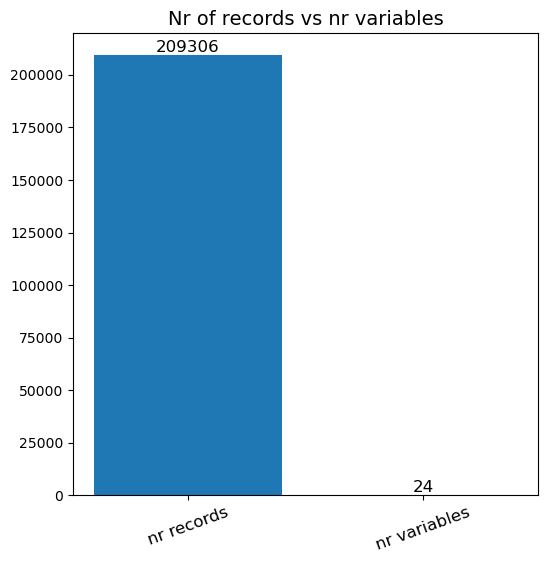
\includegraphics[width=\textwidth]{traffic_accidents_records_variables.png}
    \end{subfigure}
    \hfill
    \begin{subfigure}[b]{0.45\textwidth}
        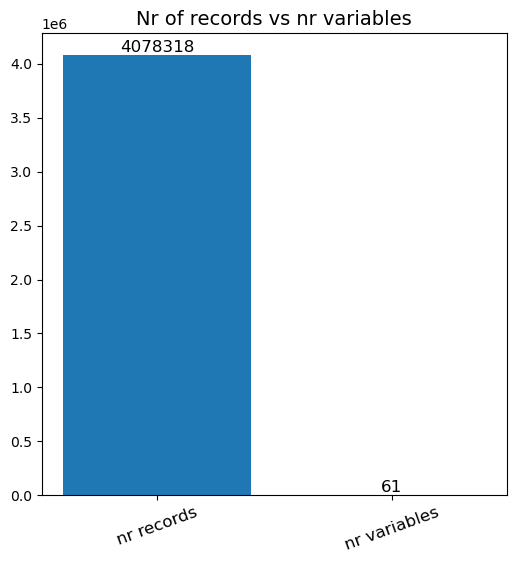
\includegraphics[width=\textwidth]{Combined_Flights_2022_records_variables.png}
    \end{subfigure}
    \caption{Nr Records x Nr variables for dataset 1 (left) and dataset 2 (right)}
\end{figure}

\begin{figure}[H]
    \centering
    \begin{subfigure}[b]{0.45\textwidth}
        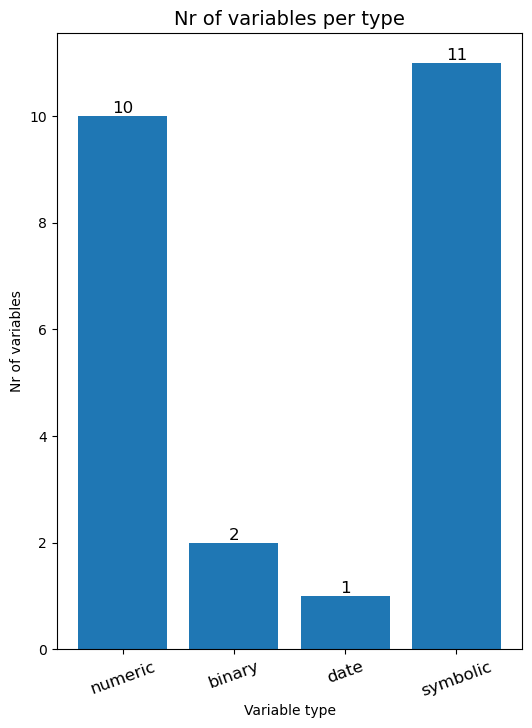
\includegraphics[width=\textwidth]{traffic_accidents_variable_types.png}
    \end{subfigure}
    \hfill
    \begin{subfigure}[b]{0.45\textwidth}
        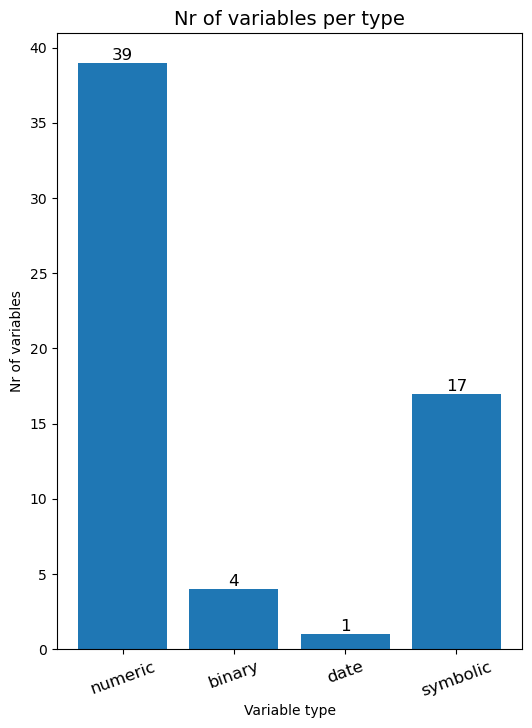
\includegraphics[width=\textwidth]{Combined_Flights_2022_variable_types.png}
    \end{subfigure}
    \caption{Nr variables per type for dataset 1 (left) and dataset 2 (right)}
\end{figure}

\begin{figure}[H]
    \centering
    \begin{subfigure}[b]{0.45\textwidth}
        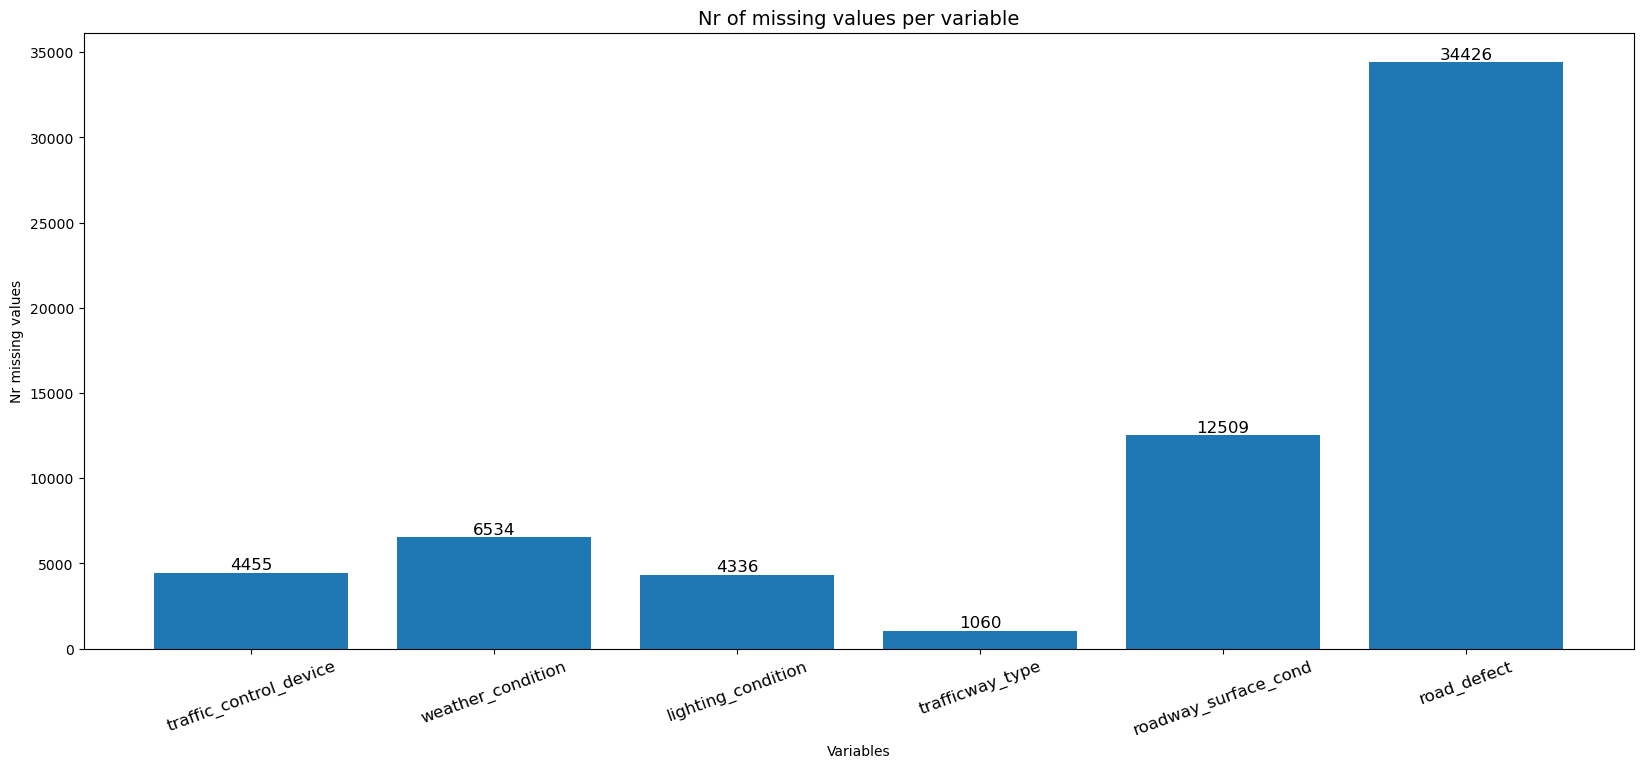
\includegraphics[width=\textwidth]{traffic_accidents_mv.png}
    \end{subfigure}
    \hfill
    \begin{subfigure}[b]{0.45\textwidth}
        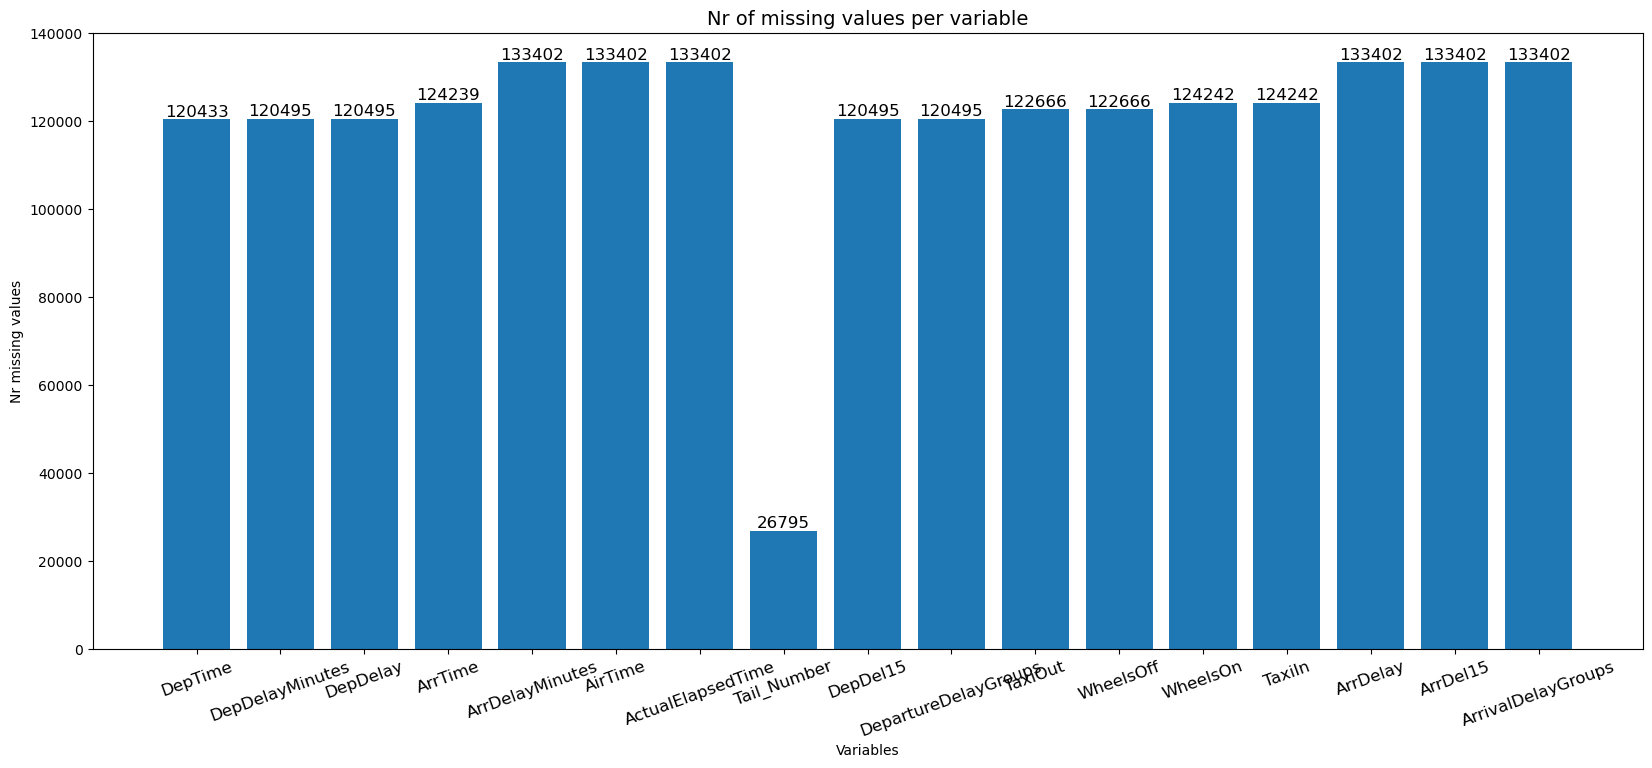
\includegraphics[width=\textwidth]{Combined_Flights_2022_mv.png}
    \end{subfigure}
    \caption{Nr missing values for dataset 1 (left) and dataset 2 (right)}
\end{figure}

\subsection*{\textit{Data Distribution}}
\ctext[RGB]{190,190,190}{Shall contain all relevant information and charts respecting to the data distribution perspective, such as each variable distribution, type, domain and range. May be used to describe any useful observation about the data, and that was used in the current project.  \textbf{Shall not exceed 500 characters.}} 

\begin{figure}[H]
    \centering
    \begin{subfigure}[b]{0.45\textwidth}
        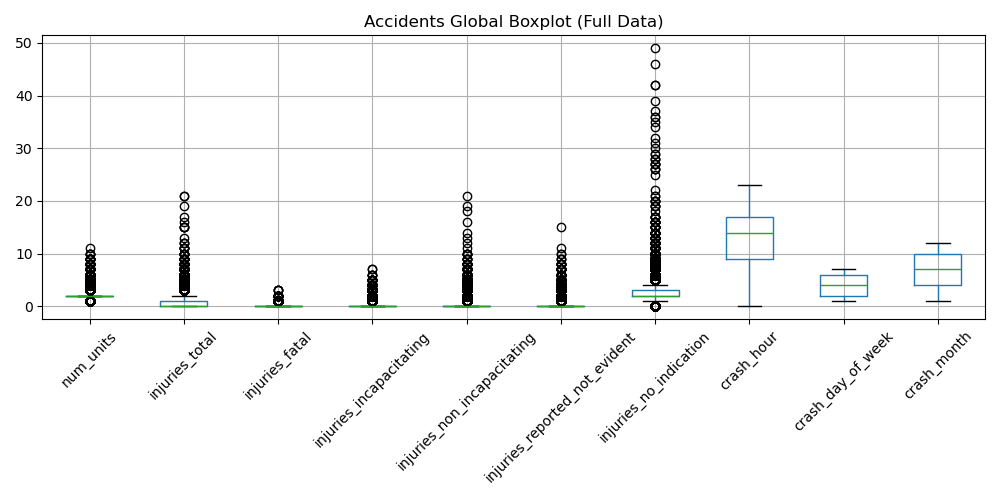
\includegraphics[width=\textwidth]{accidents_global_boxplot.png}
    \end{subfigure}
    \hfill
    \begin{subfigure}[b]{0.45\textwidth}
        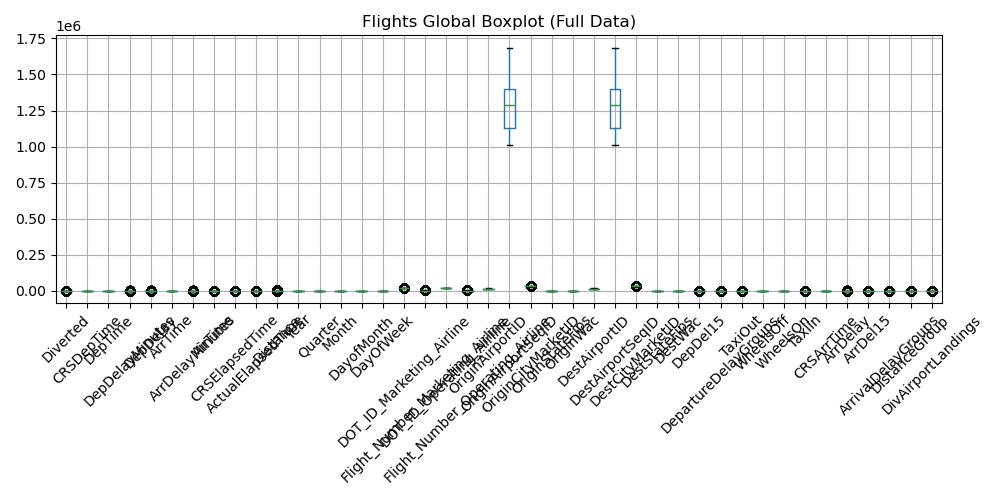
\includegraphics[width=\textwidth]{flights_global_boxplot.png}
    \end{subfigure}
    \caption{Global boxplots dataset 1 (left) and dataset 2 (right)}
\end{figure}

\begin{figure}[H]
\centering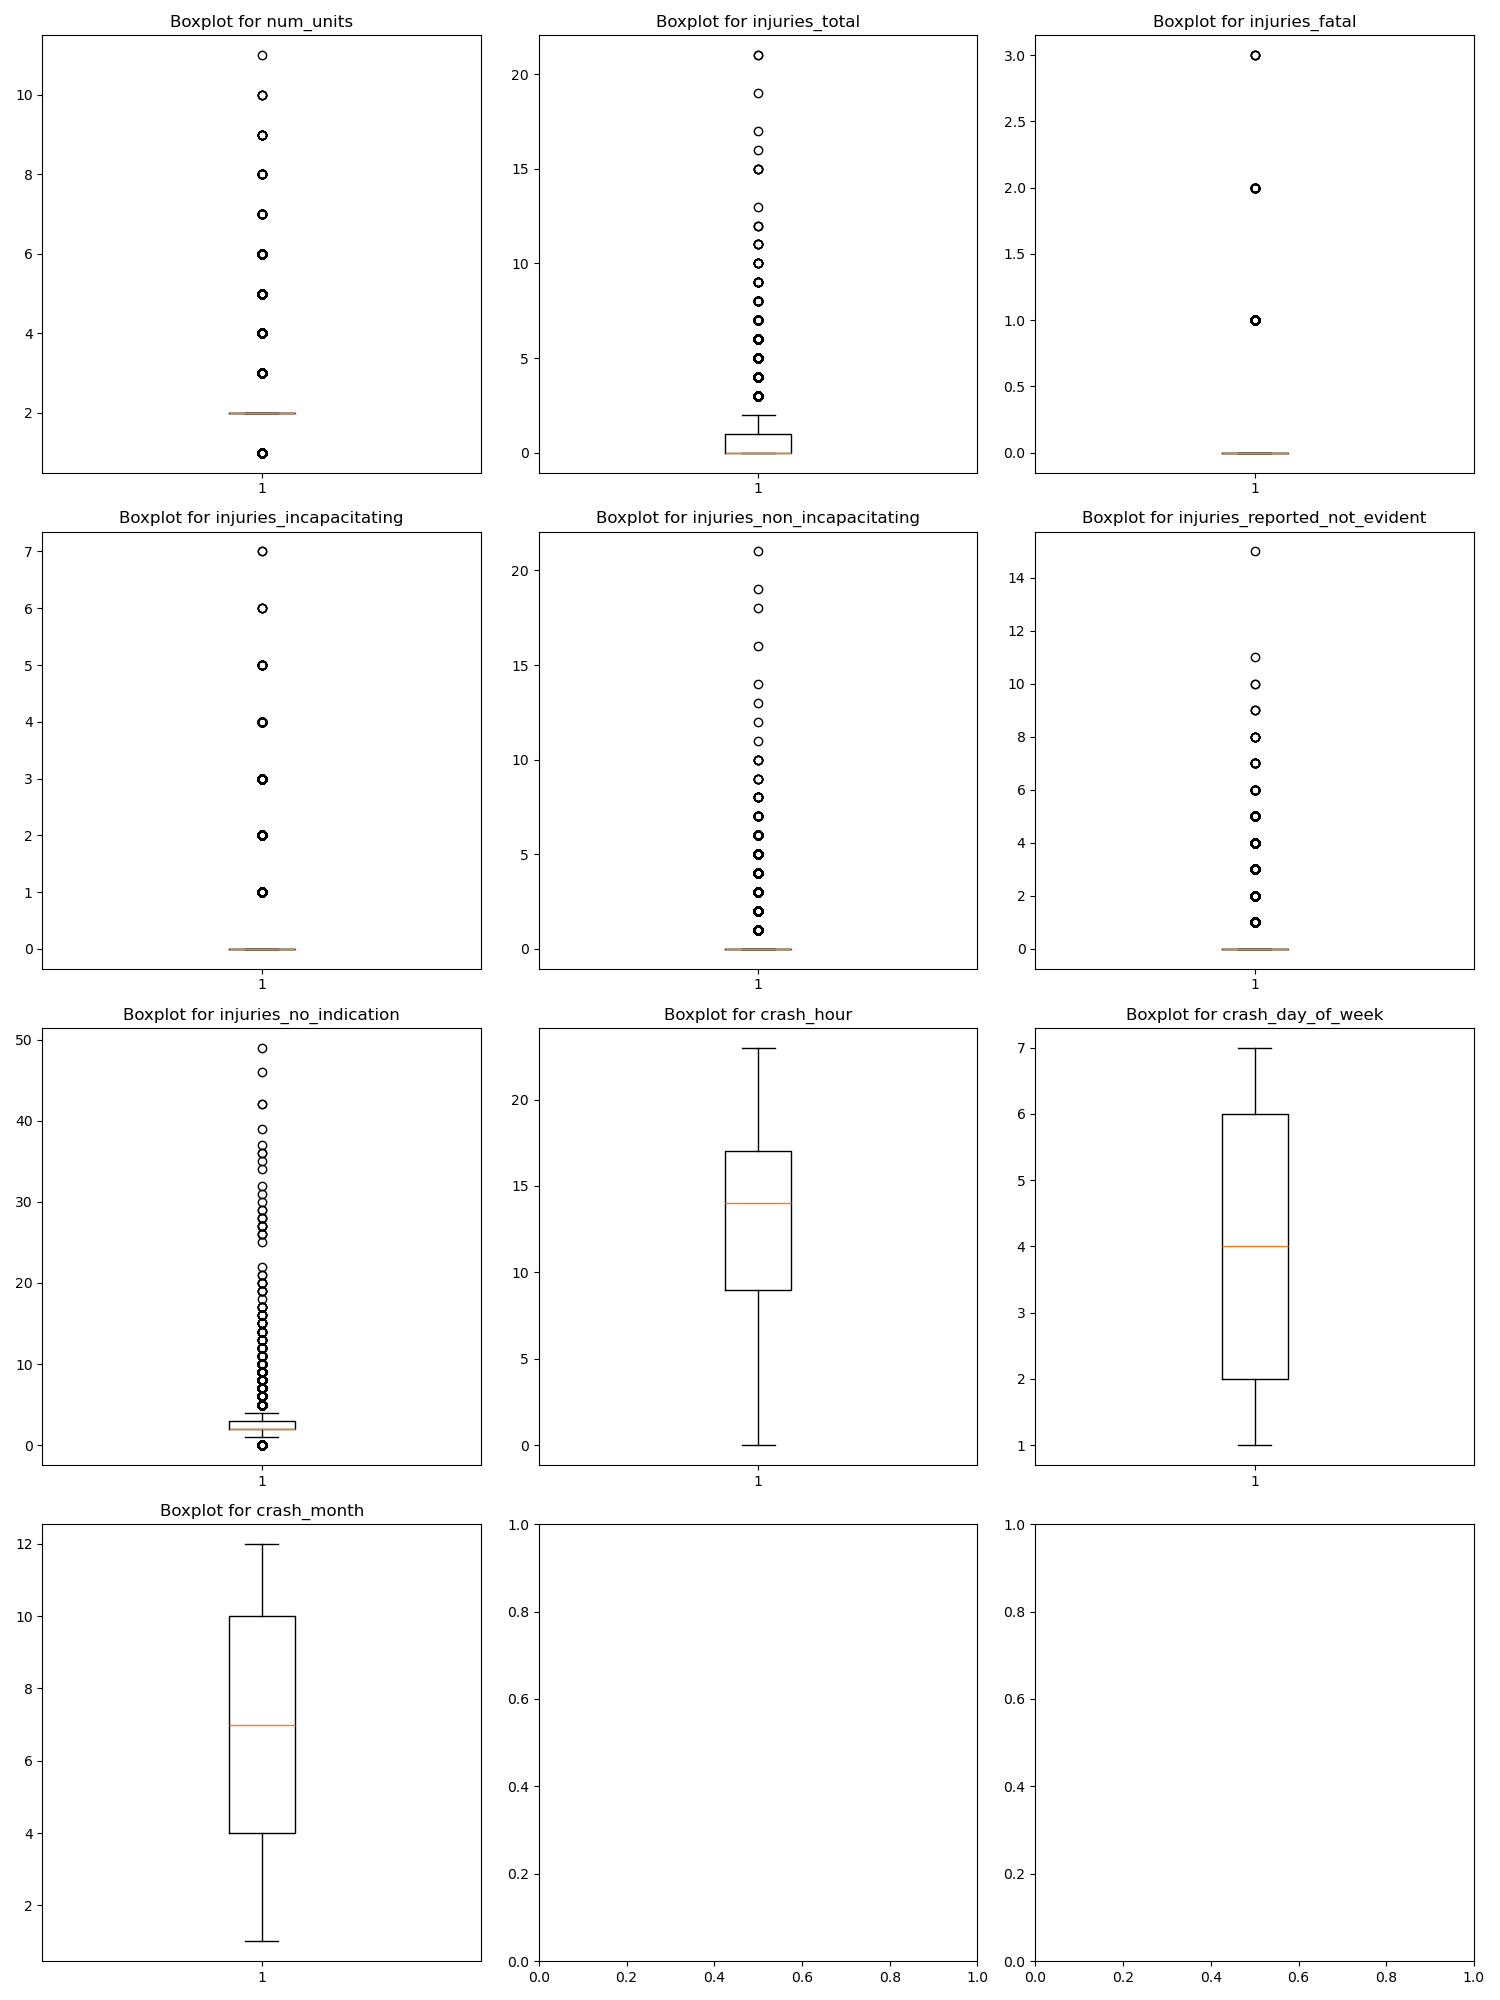
\includegraphics[width=0.7\textwidth]{accidents_single_boxplots.png}
\caption{Single variables boxplots for dataset 1}
\end{figure}

\begin{figure}[H]
\centering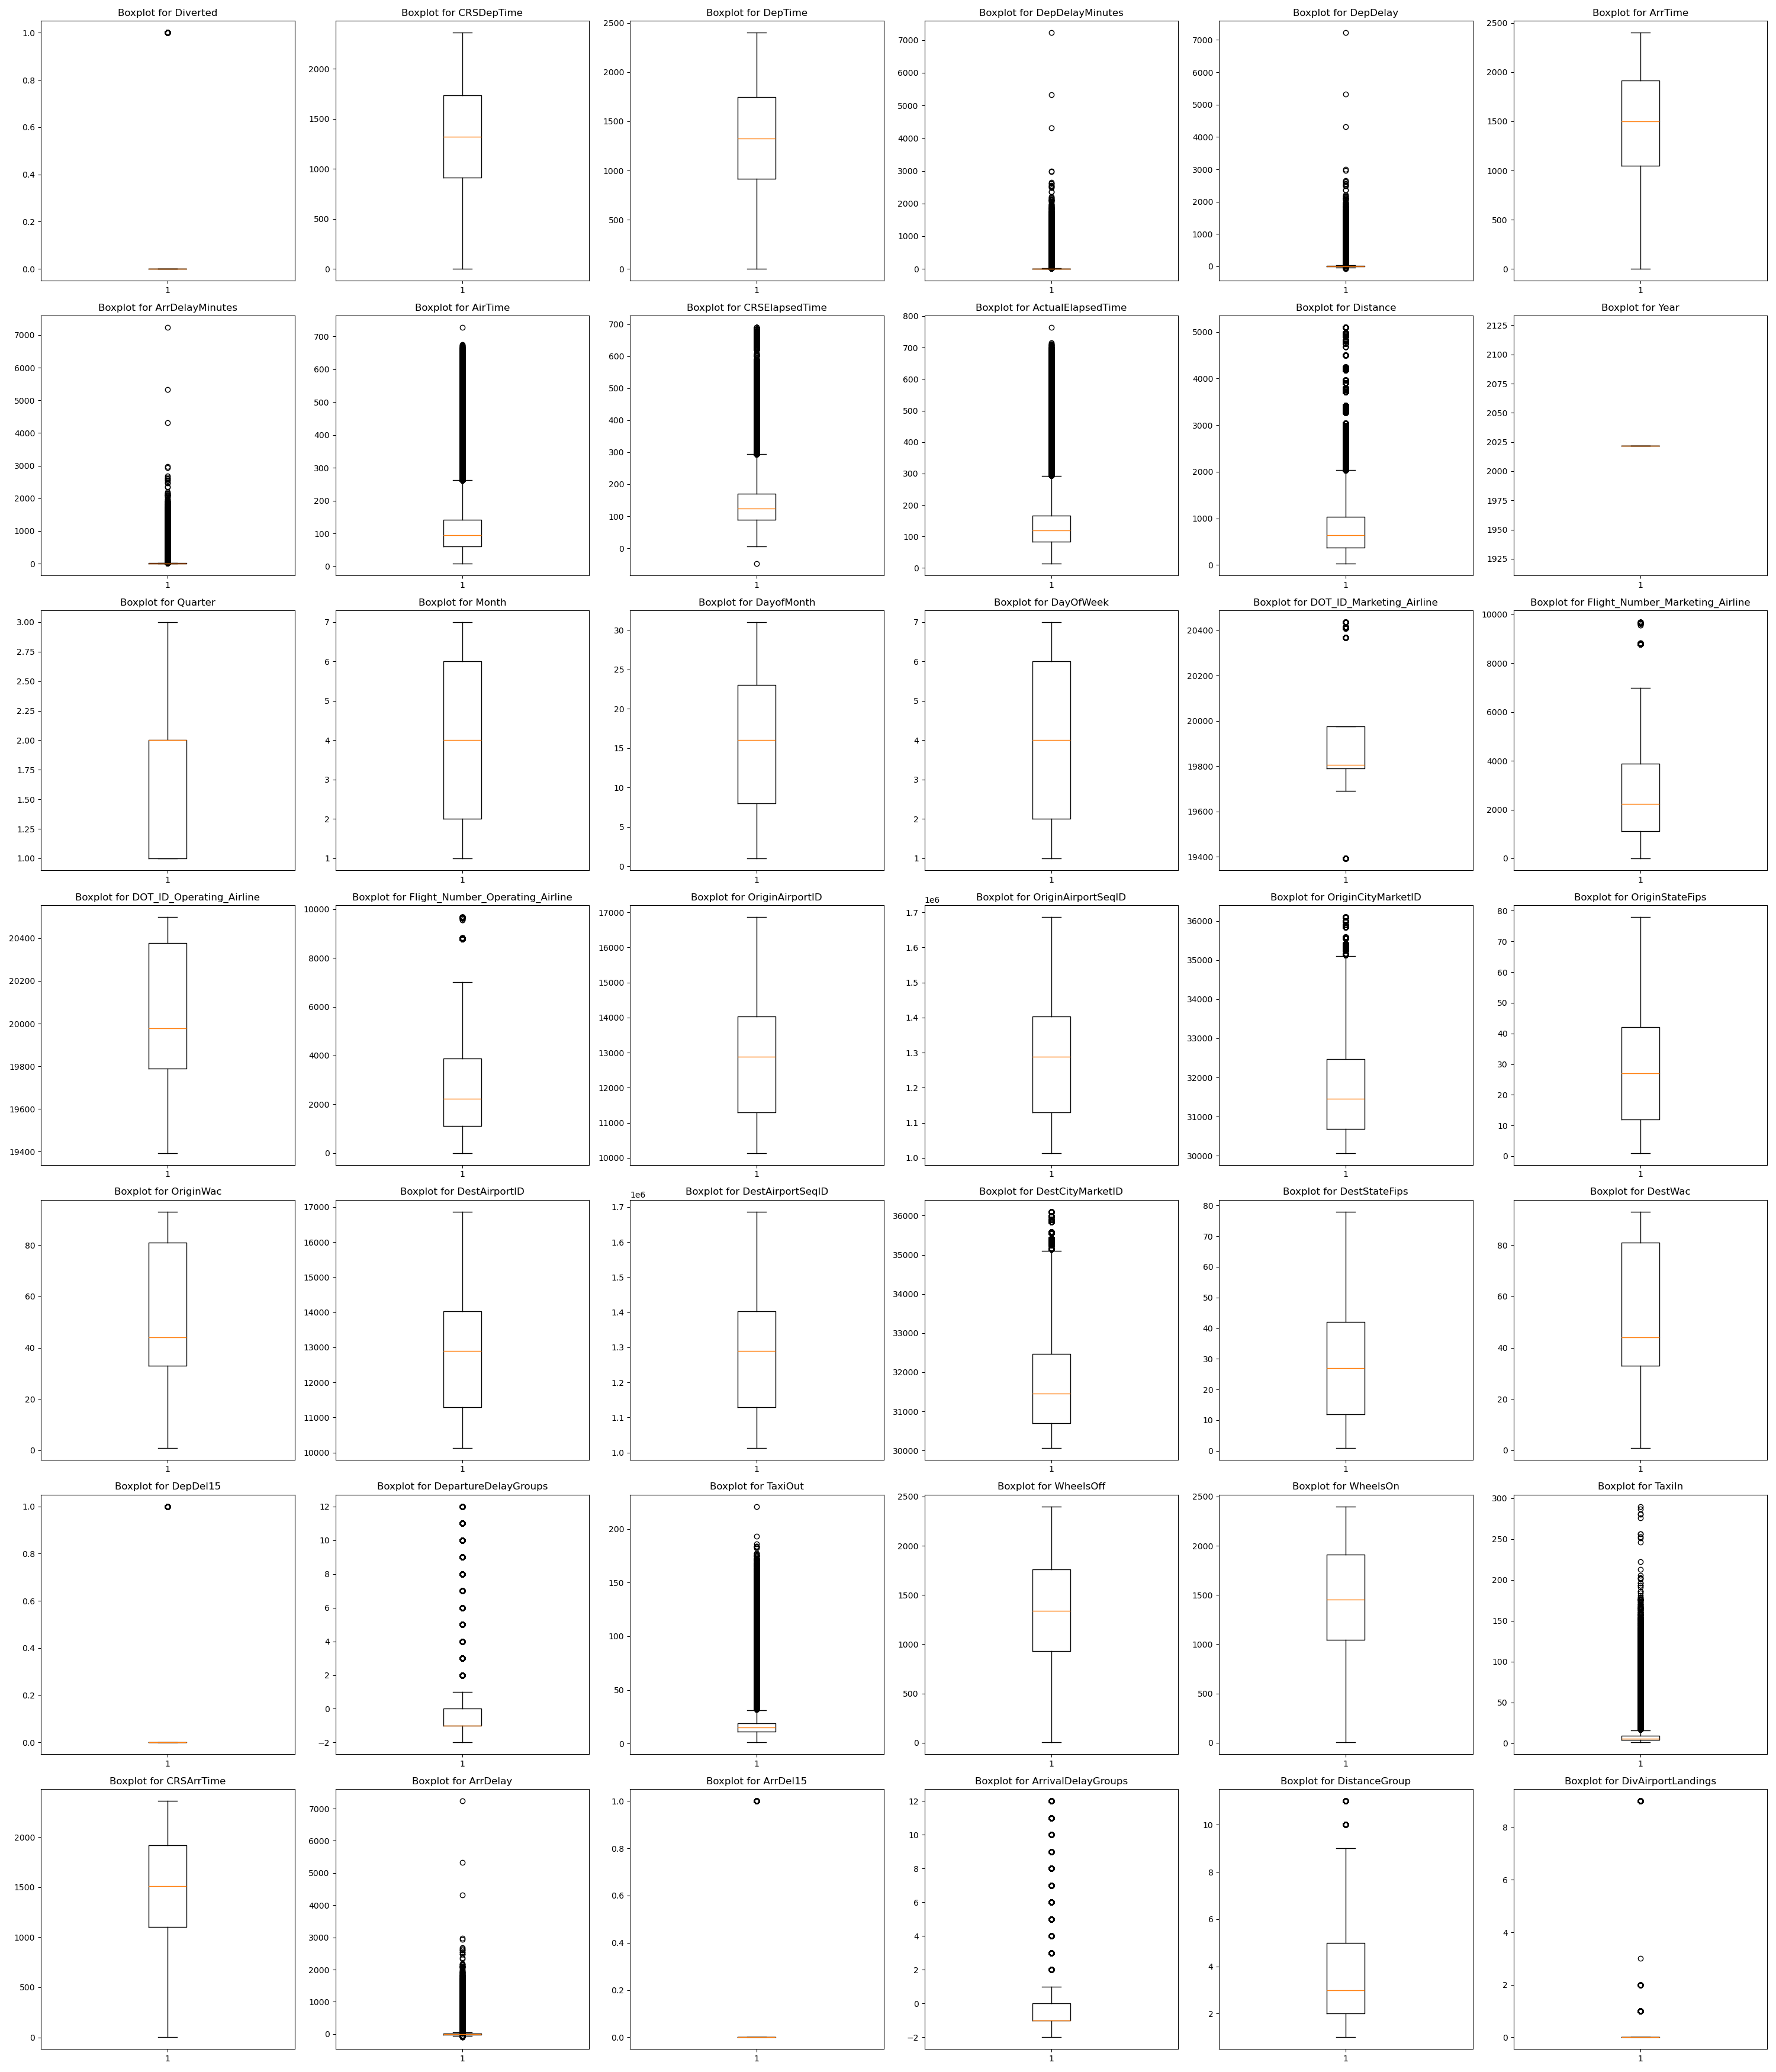
\includegraphics[width=0.7\textwidth]{flights_single_boxplots.png}
\caption{Single variables boxplots for dataset 2}
\end{figure}

\begin{figure}[H]
\centering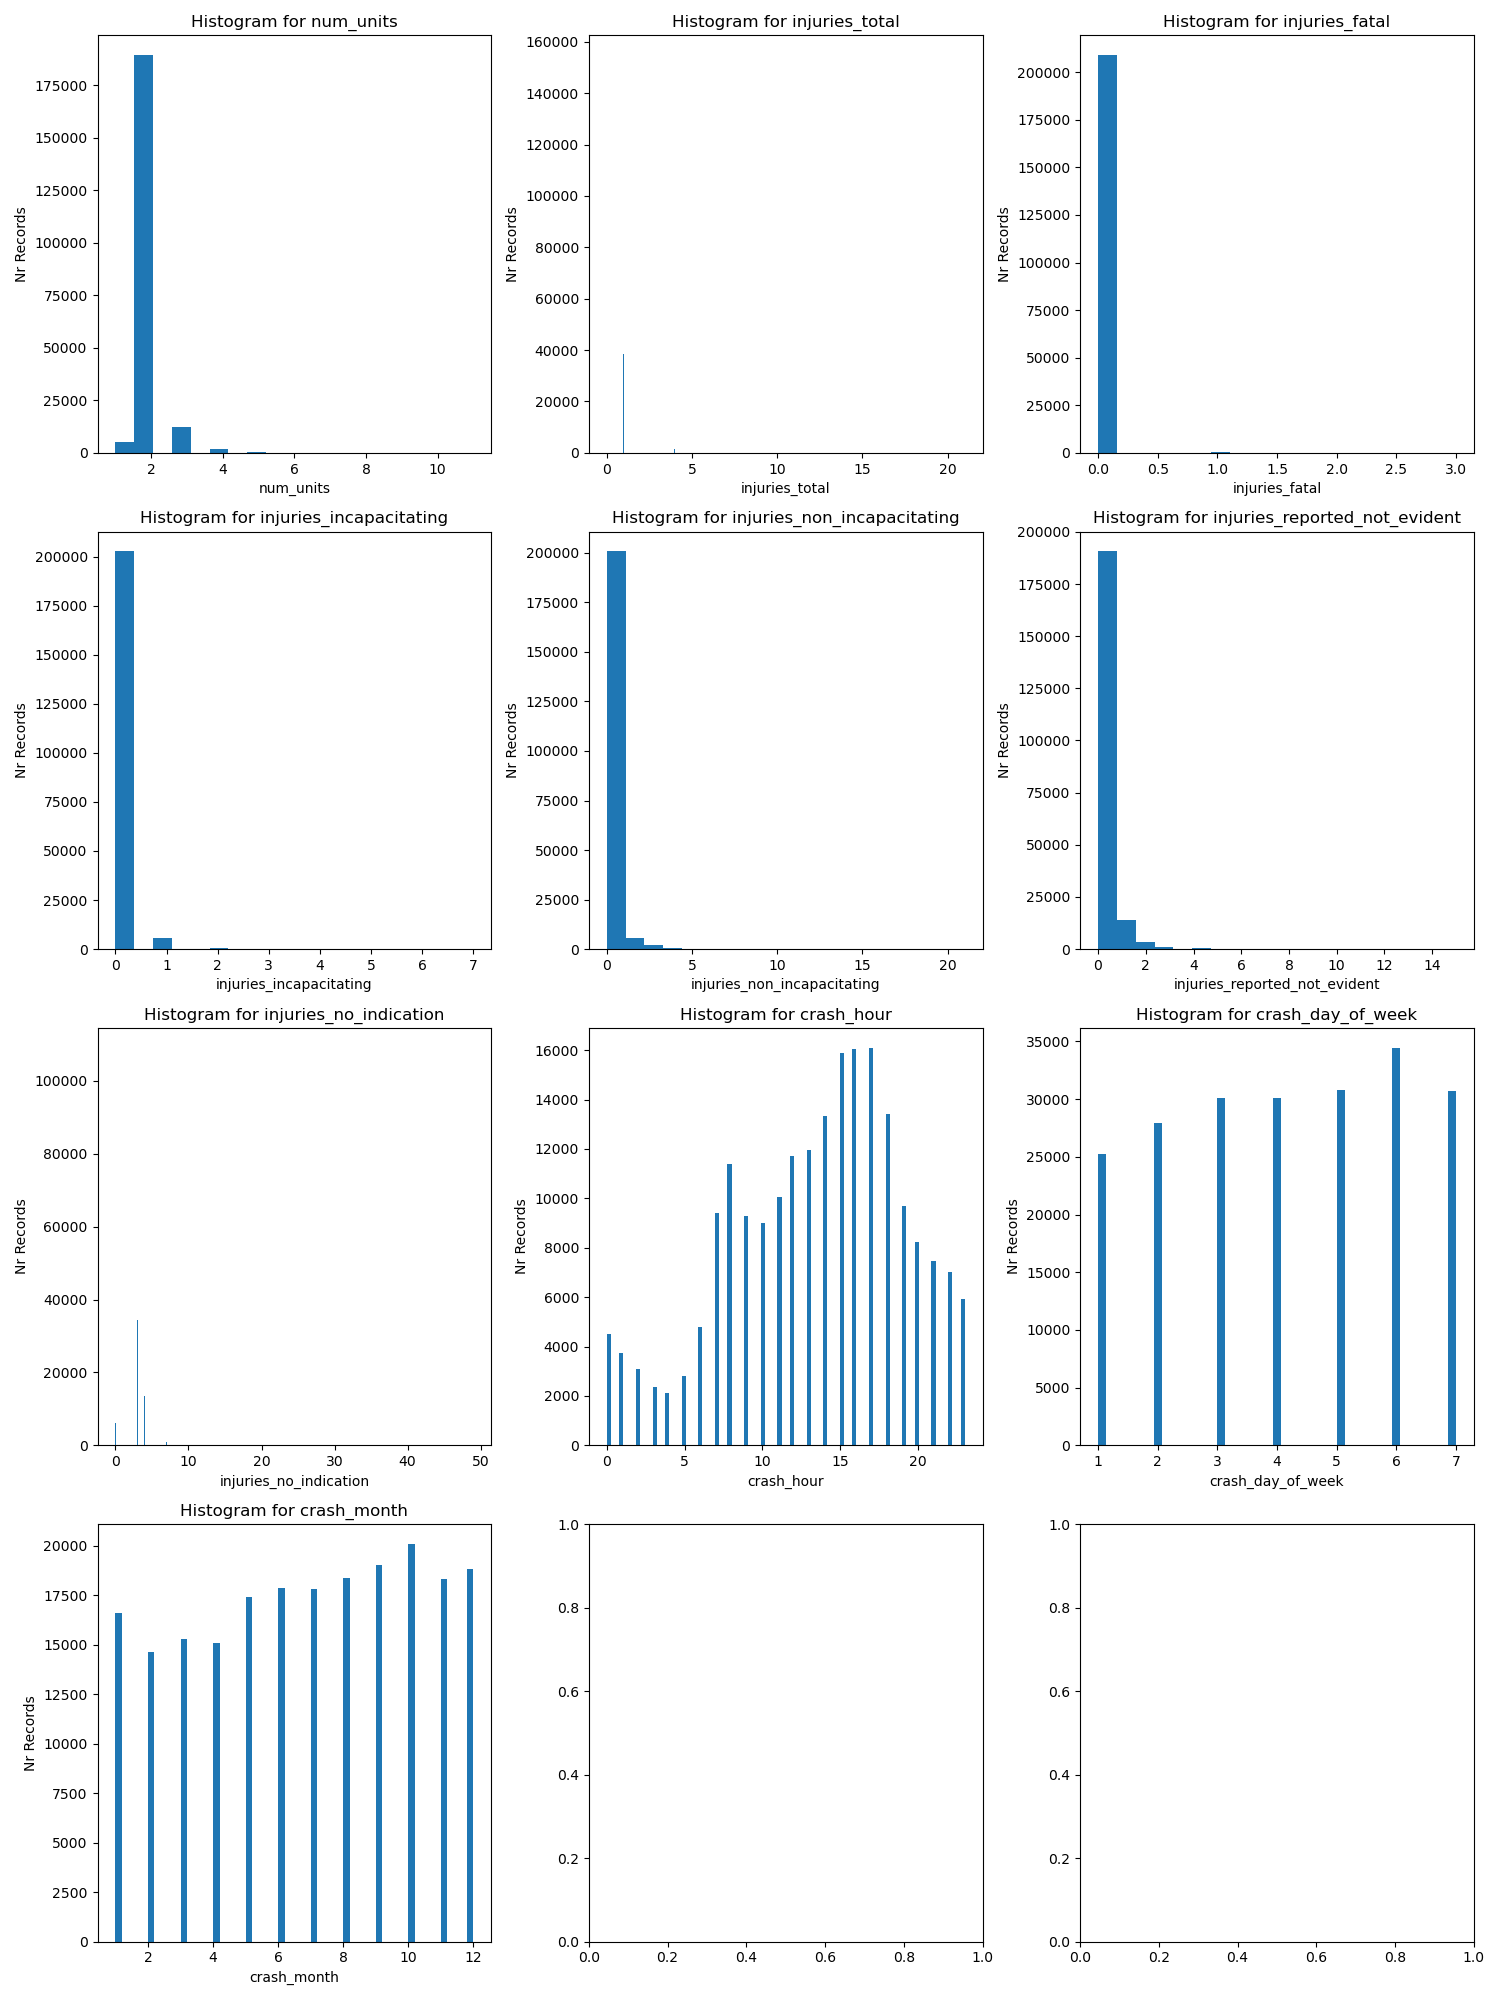
\includegraphics[width=0.7\textwidth]{accidents_single_histograms.png}
\caption{Histograms for dataset 1} %(with distributions is enough)
\end{figure}

\begin{figure}[H]
\centering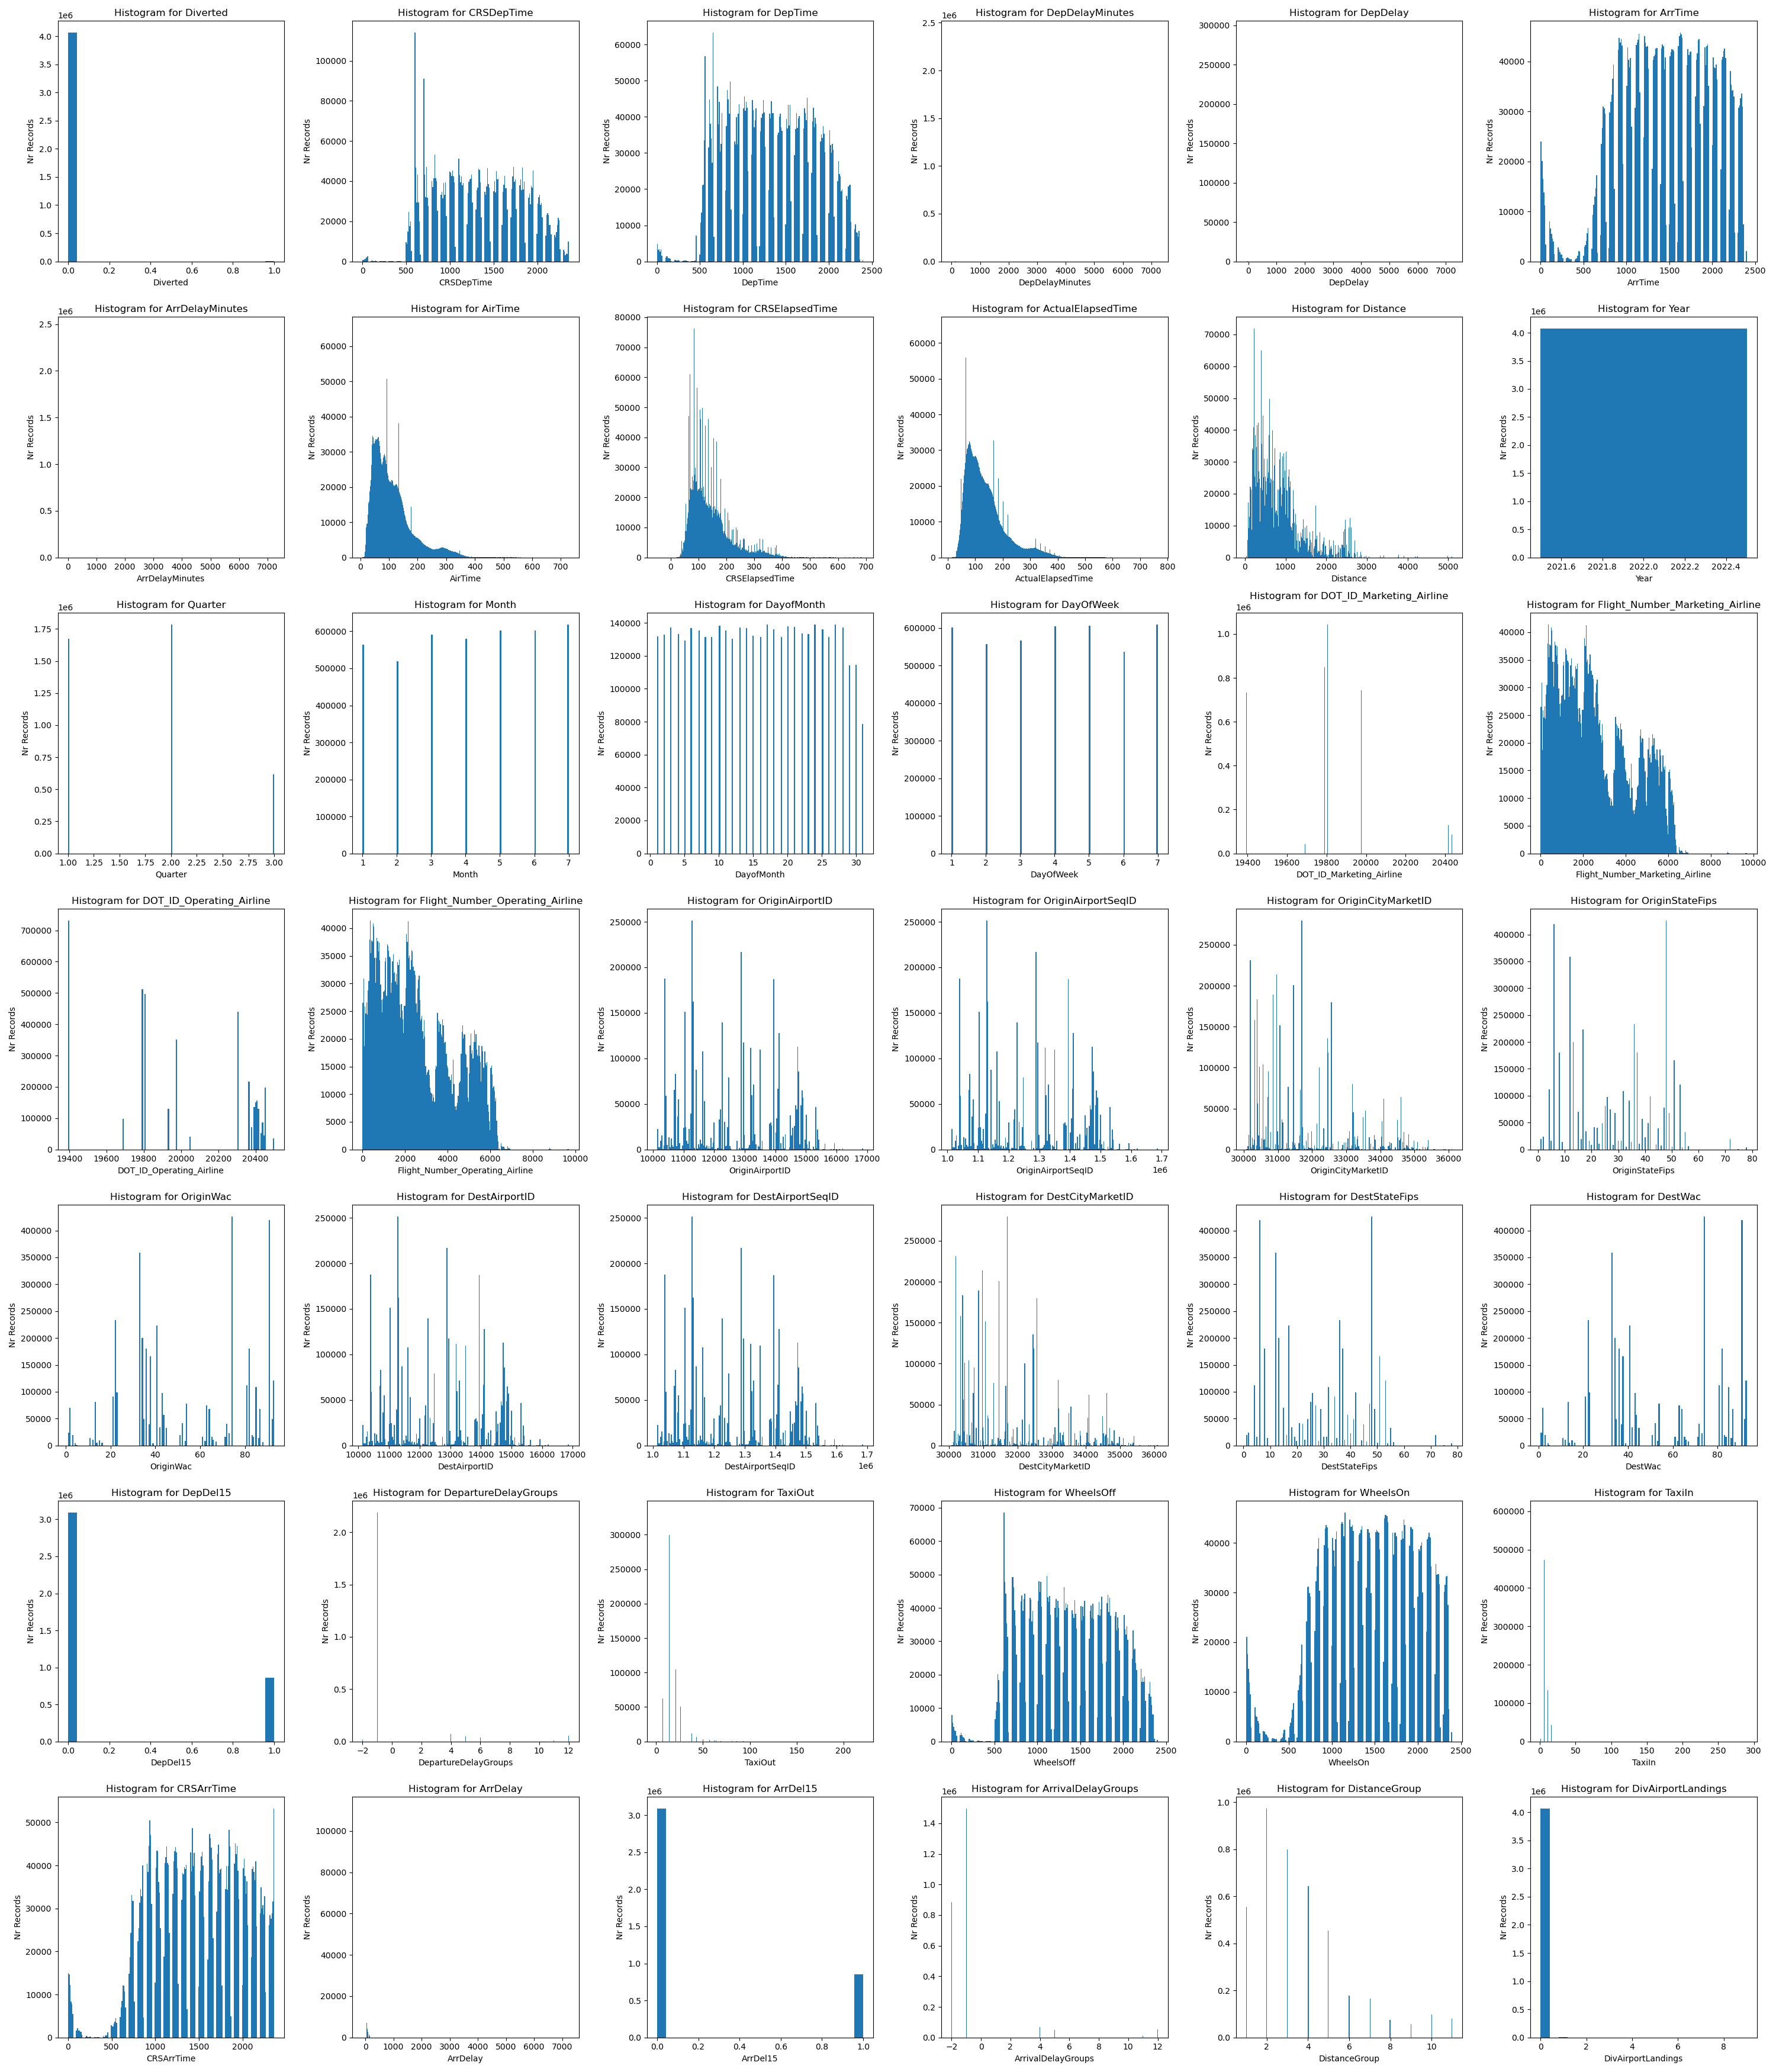
\includegraphics[width=0.7\textwidth]{flights_single_histograms.png}
\caption{Histograms for dataset 2} %(with distributions is enough)
\end{figure}

\begin{figure}[H]
\centering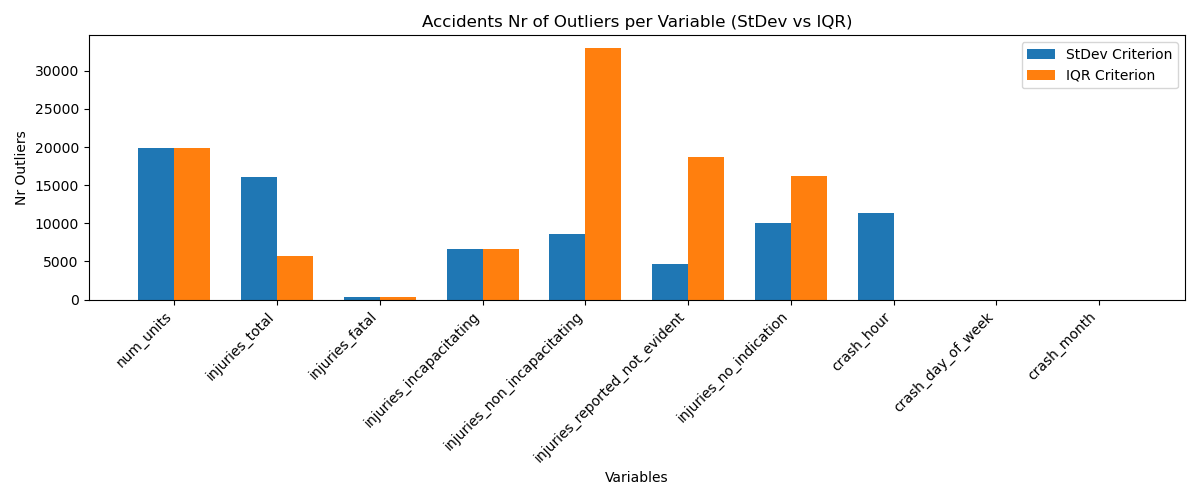
\includegraphics[width=0.9\textwidth]{accidents_outliers_comparison.png}
\caption{Outliers study dataset 1}
\end{figure}

\begin{figure}[H]
\centering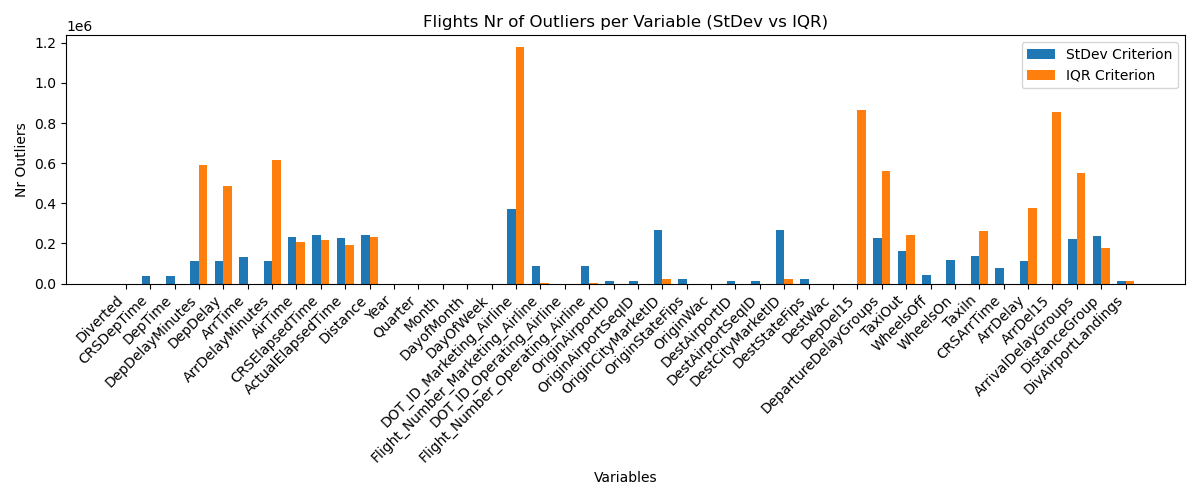
\includegraphics[width=0.9\textwidth]{flights_outliers_comparison.png}
\caption{Outliers study dataset 2}
\end{figure}

\begin{figure}[H]
\centering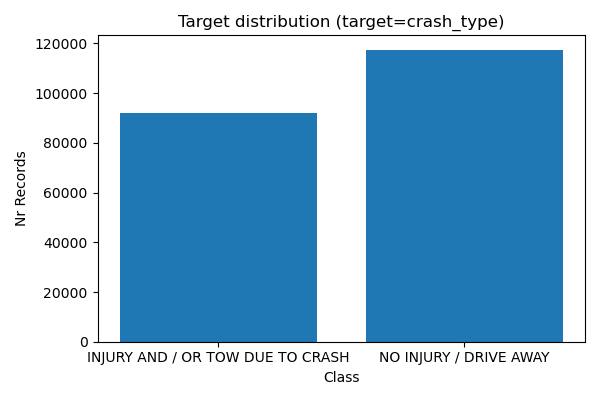
\includegraphics[width=0.9\textwidth]{accidents_class_distribution.png}
\caption{Class distribution for dataset 1}
\end{figure}

\begin{figure}[H]
\centering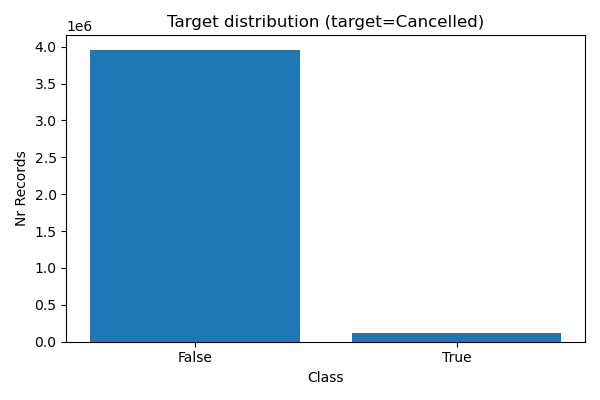
\includegraphics[width=0.9\textwidth]{flights_class_distribution.png}
\caption{Class distribution for dataset 2}
\end{figure}

\subsection*{\textit{Data Granularity}}
\ctext[RGB]{190,190,190}{Shall contain all relevant information and charts respecting to the data granularity perspective, such as the impact of different granularities considered for each variable. May present additional taxonomies if needed.  \textbf{Shall not exceed 500 characters.}}

\begin{figure}[H]
\centering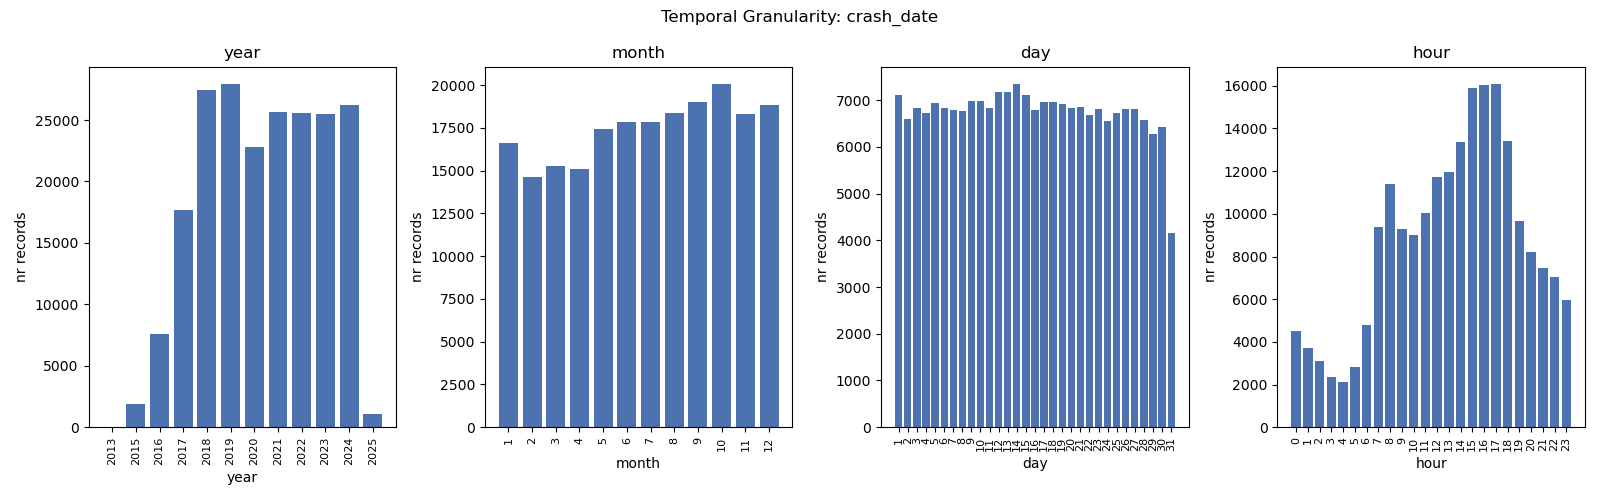
\includegraphics[width=0.9\textwidth]{accidents_granularity_date.png}
\caption{Granularity analysis for dataset 1}
\end{figure}

\begin{figure}[H]
\centering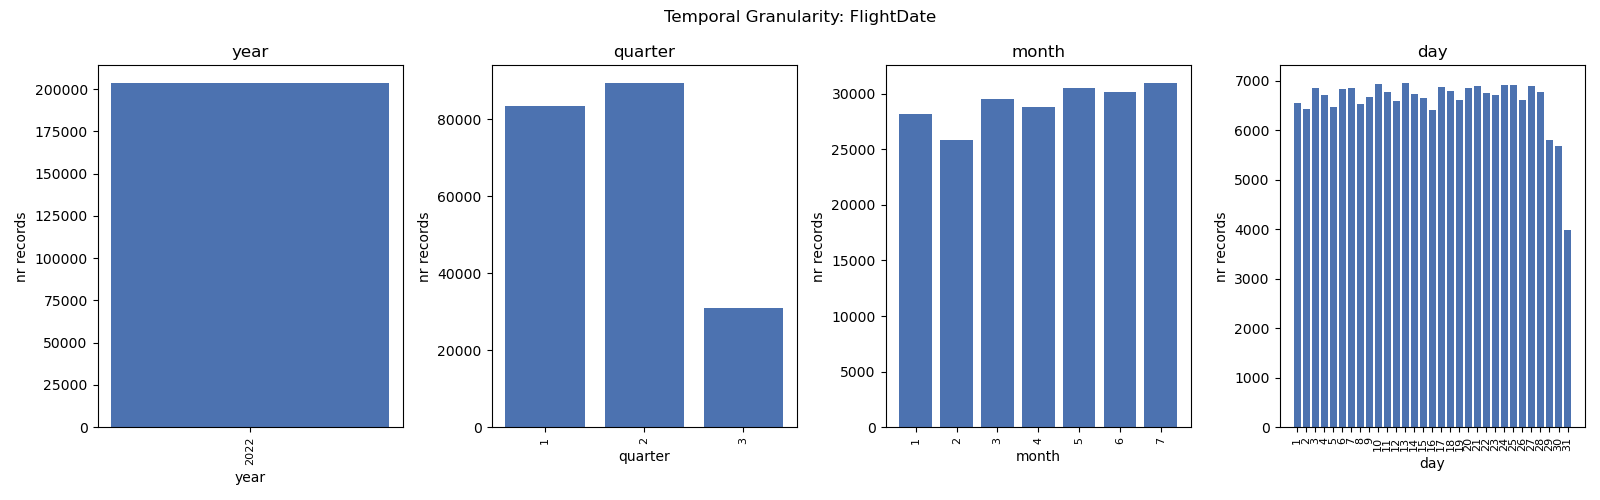
\includegraphics[width=0.9\textwidth]{flights_granularity_date.png}
\caption{Granularity analysis for dataset 2}
\end{figure}

\subsection*{\textit{Data Sparsity}}
\ctext[RGB]{190,190,190}{Shall contain all relevant information and charts respecting to the data sparsity perspective, such as domain coverage and correlation among variables.  \textbf{Shall not exceed 500 characters.}}

\begin{figure}[H]
\centering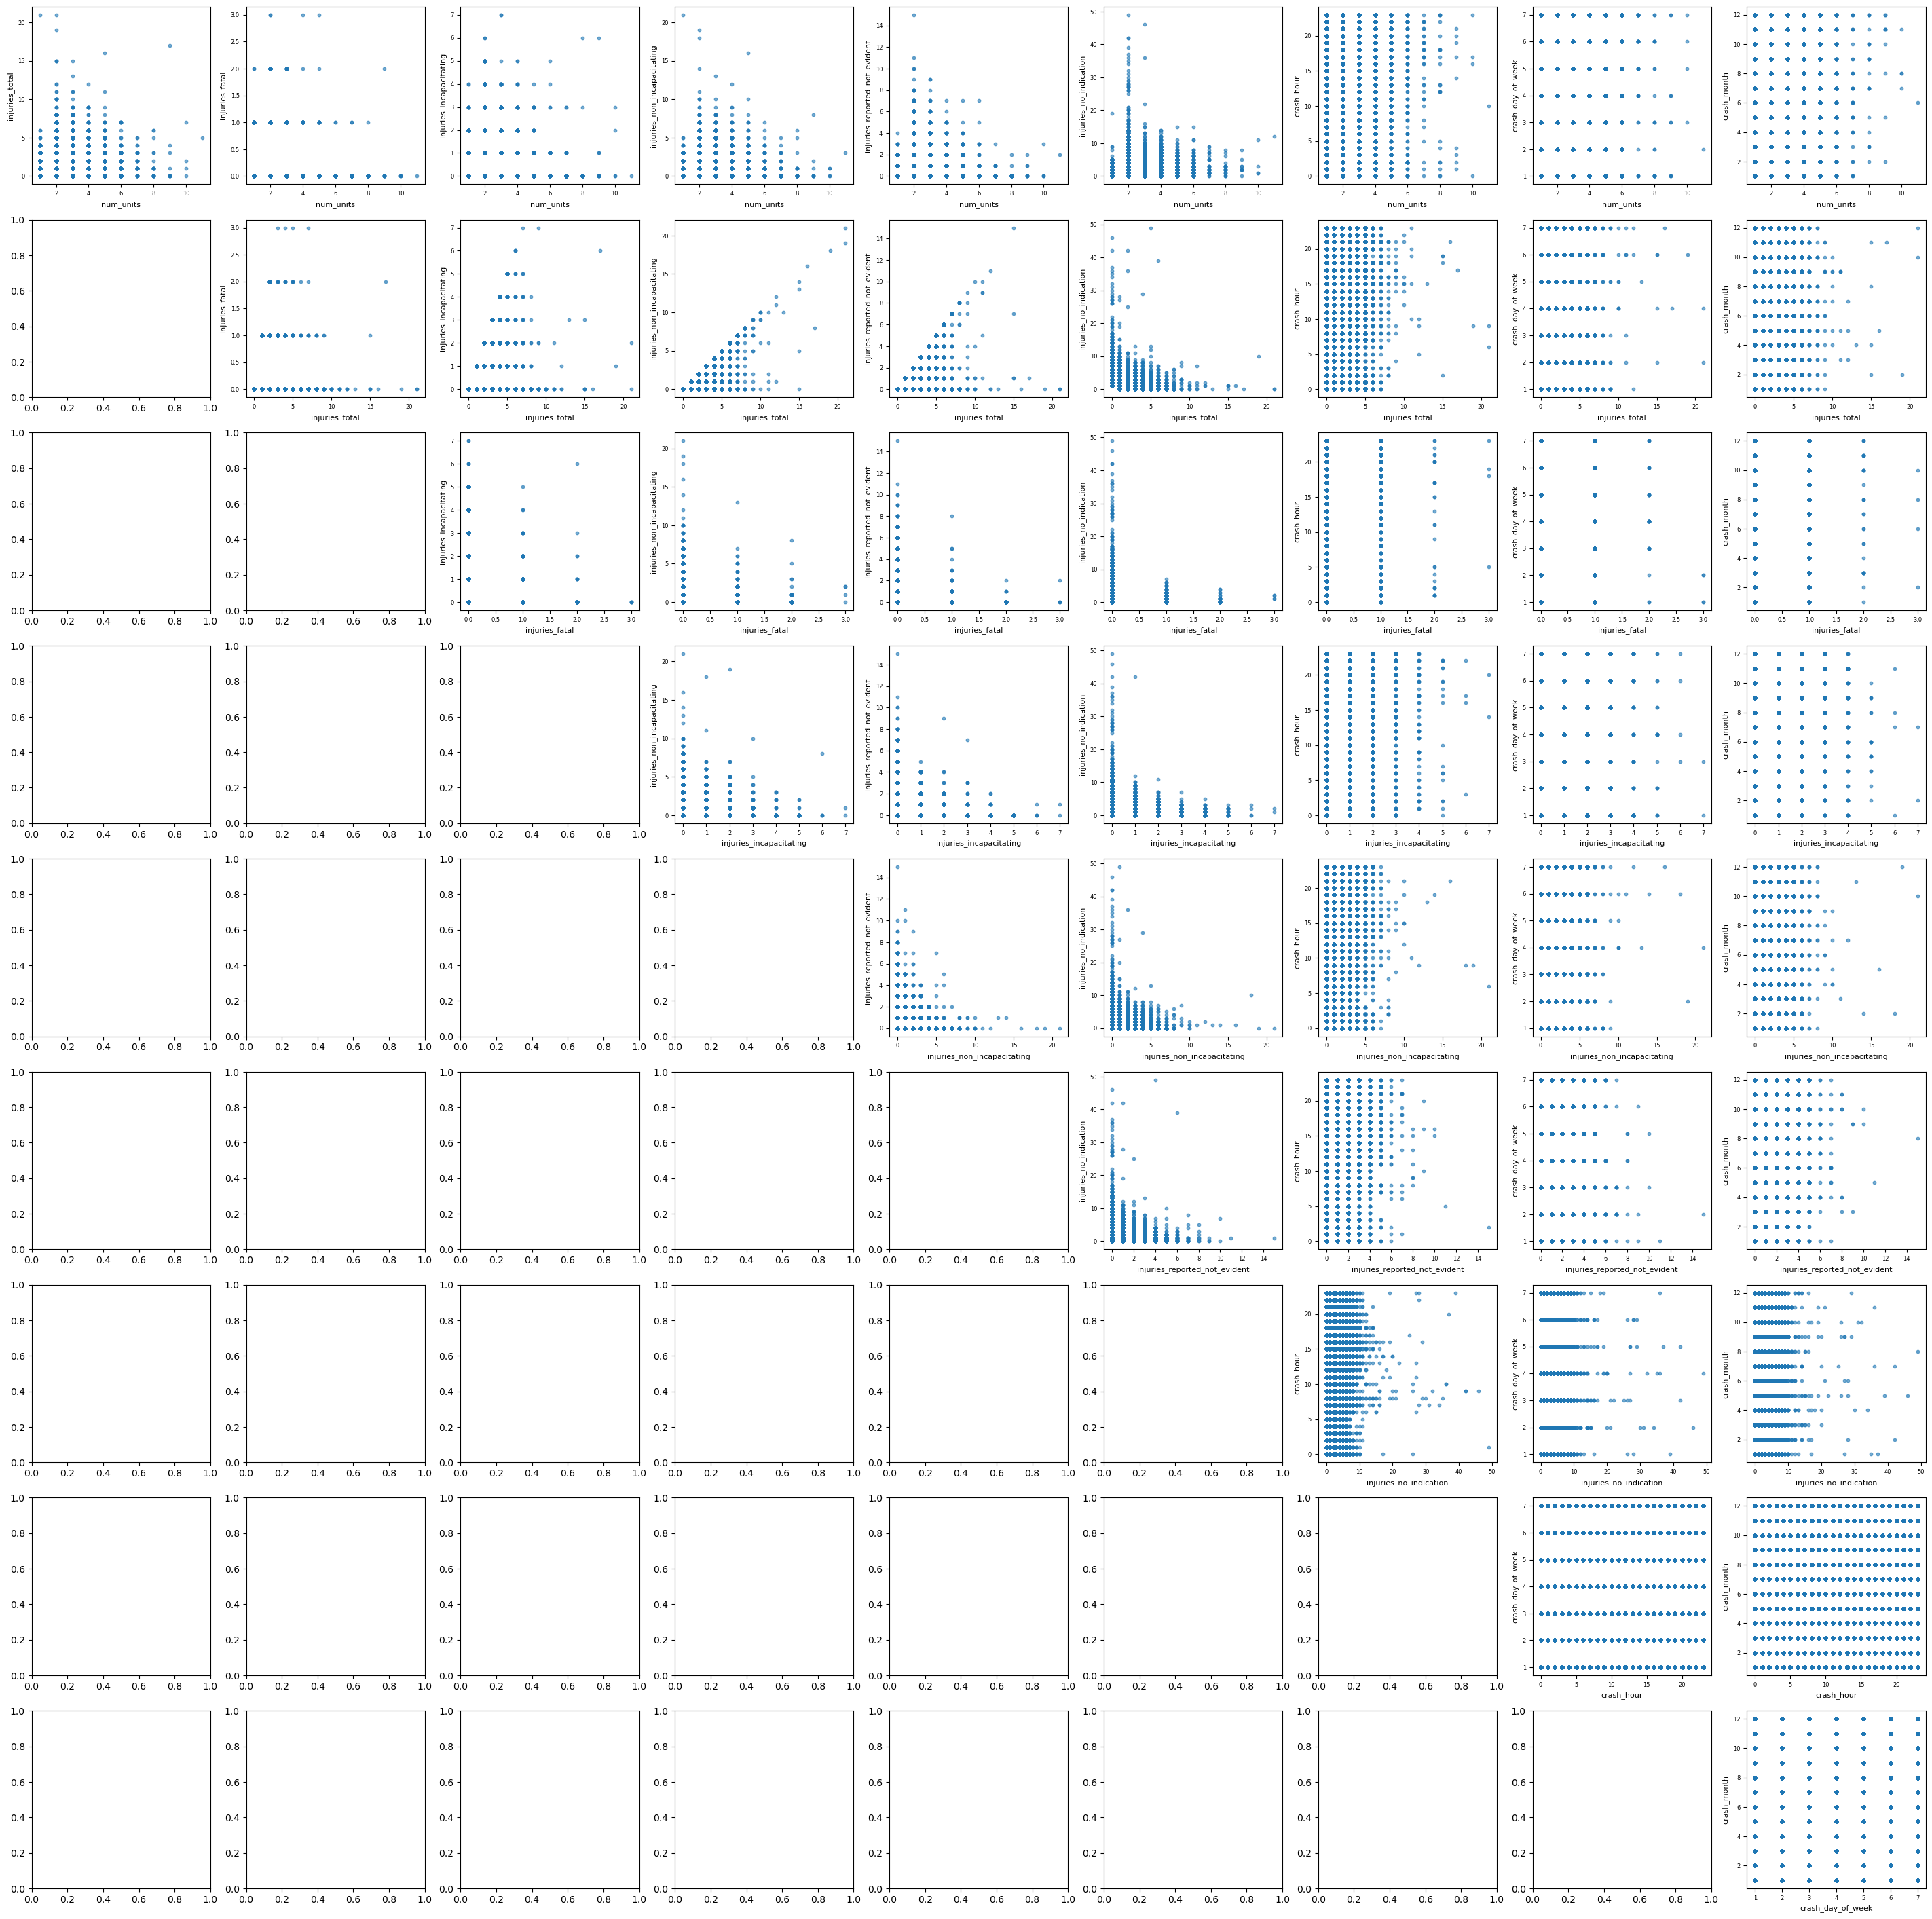
\includegraphics[width=0.9\textwidth]{accidents_sparsity_study.png}
\caption{Sparsity analysis for dataset 1}
\end{figure}

\begin{figure}[H]
\centering\includegraphics[width=0.9\textwidth]{flights_sparsity_study.png}
\caption{Sparsity analysis for dataset 2}
\end{figure}

\begin{figure}[H]
\centering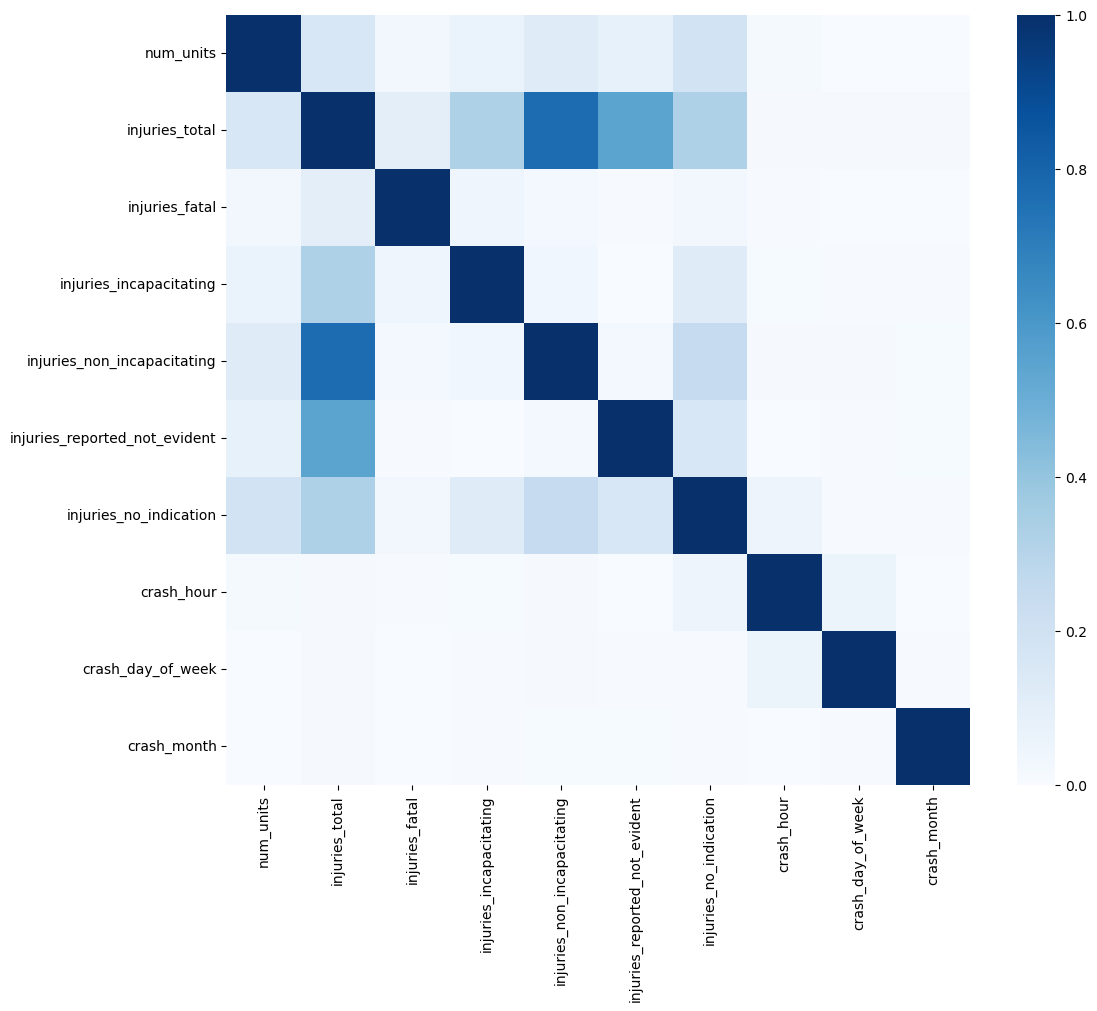
\includegraphics[width=0.9\textwidth]{accidents_correlation_analysis.png}
\caption{Correlation analysis for dataset 1}
\end{figure}

\begin{figure}[H]
\centering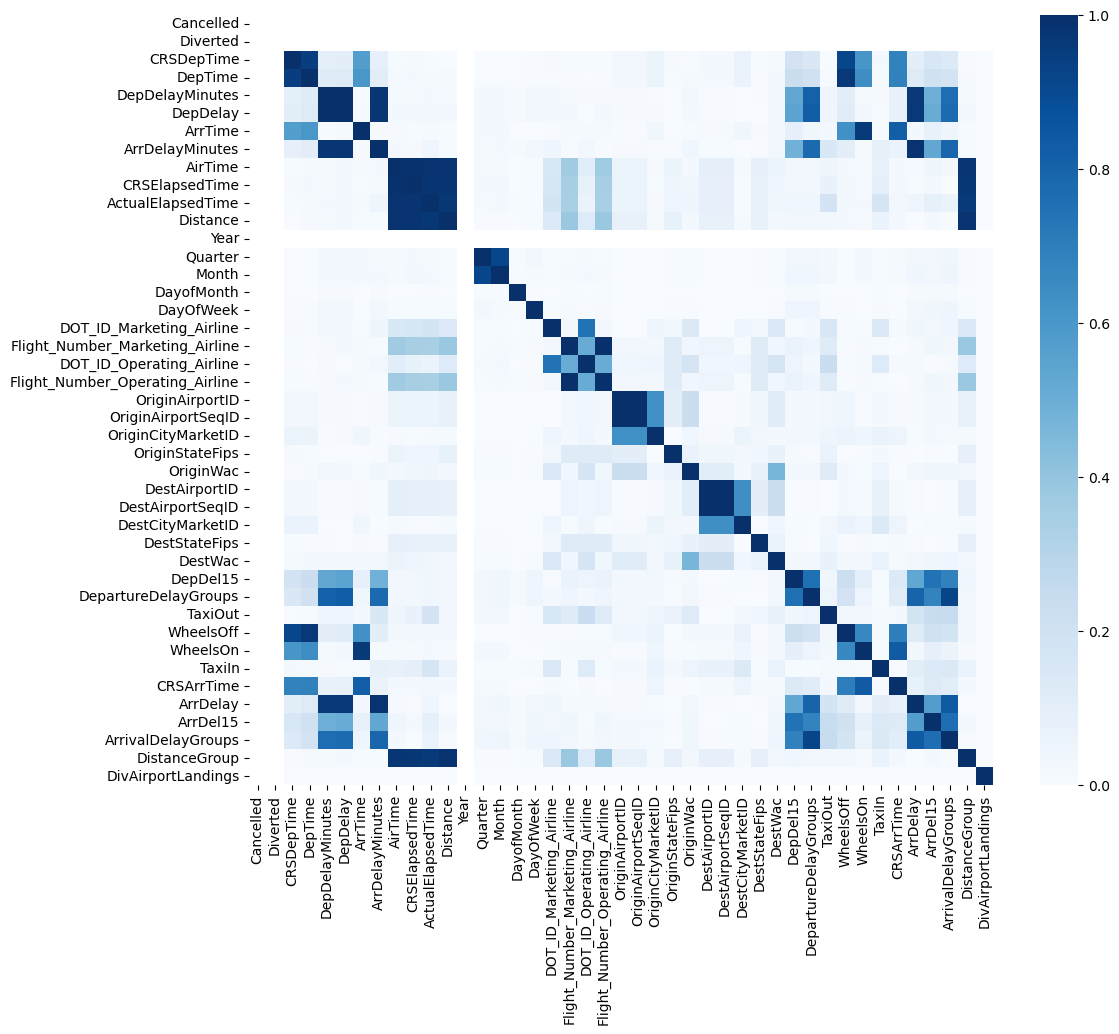
\includegraphics[width=0.9\textwidth]{flights_correlation_analysis.png}
\caption{Correlation analysis for dataset 2}
\end{figure}

\section{DATA PREPARATION}

\subsection*{\textit{Variables Encoding}}
\ctext[RGB]{190,190,190}{Shall contain all relevant information respecting to the transformation of variables. The list of variables under each one of the transformations, shall be presented. If not applied explain the reason for that, based on data characteristics.  \textbf{Shall not exceed 500 characters \textit{for each dataset.}}}

\subsection*{\textit{Missing Value Imputation}}
\ctext[RGB]{190,190,190}{Shall contain all relevant information and charts respecting to missing values imputation, such as the choices made and the impact of the different approaches on modelling results. Shall also clearly reveal the approach selected to proceed with the processing. If not applied explain the reason for that, based on data characteristics.  \textbf{Shall not exceed 500 characters.}}

\begin{figure}[H]
\centering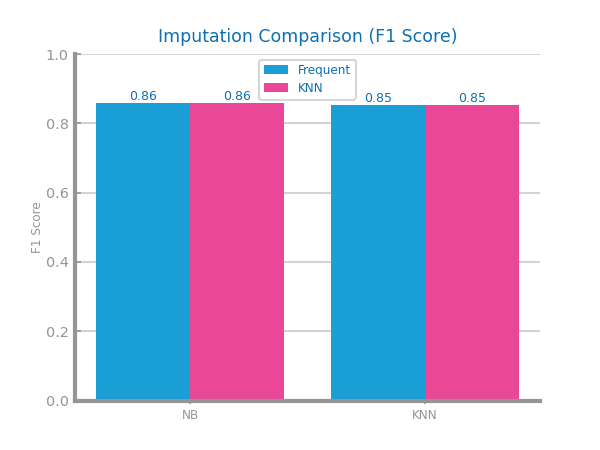
\includegraphics[width=0.9\textwidth]{2_imputation_comparison.png}
\caption{Missing values imputation results with different approaches for dataset 1}
\end{figure}

\begin{figure}[H]
\centering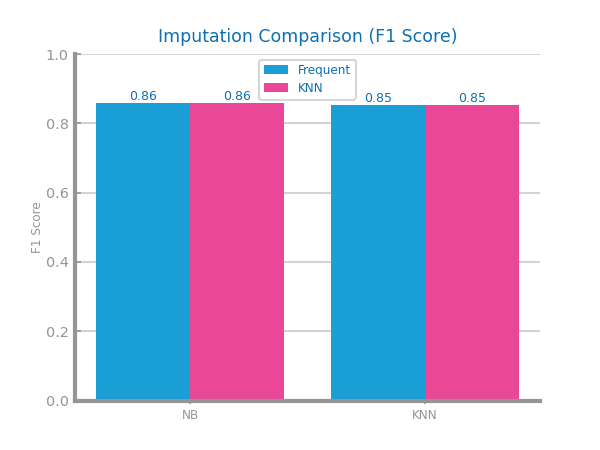
\includegraphics[width=0.9\textwidth]{2_imputation_comparison.png}
\caption{Missing values imputation results with different approaches for dataset 2}
\end{figure}

\subsection*{\textit{Outliers Treatment}}
\ctext[RGB]{190,190,190}{Shall contain all relevant information and charts respecting to outliers imputation, such as the choices made and the impact of the different approaches on modelling results. Shall also clearly reveal the approach selected to proceed with the processing. If not applied explain the reason for that, based on data characteristics.  \textbf{Shall not exceed 500 characters.}}

\begin{figure}[H]
\centering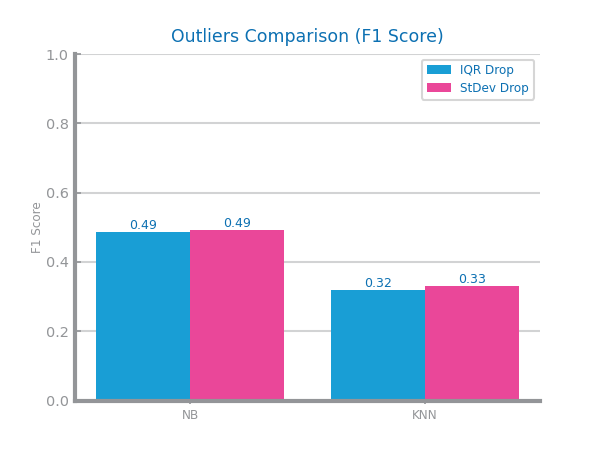
\includegraphics[width=0.9\textwidth]{3_outliers_comparison.png}
\caption{Outliers imputation results with different approaches for dataset 1}
\end{figure}

\begin{figure}[H]
\centering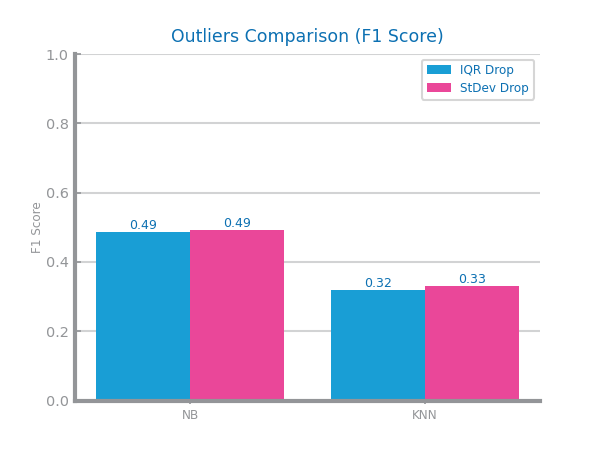
\includegraphics[width=0.9\textwidth]{3_outliers_comparison.png}
\caption{Outliers imputation results with different approaches for dataset 2}
\end{figure}

\subsection*{\textit{Scaling}}
\ctext[RGB]{190,190,190}{Shall contain all relevant information and charts respecting to scaling transformation, such as the choices made and the impact of the different approaches on modelling results. Shall also clearly reveal the approach selected to proceed with the processing. If not applied explain the reason for that, based on data characteristics.  \textbf{Shall not exceed 200 characters.}}

\begin{figure}[H]
\centering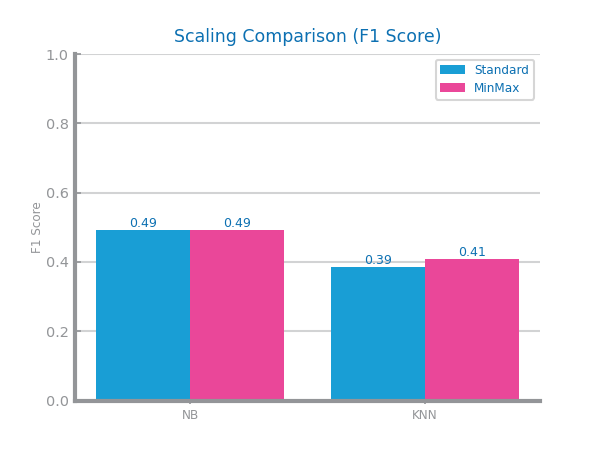
\includegraphics[width=0.9\textwidth]{4_scaling_comparison.png}
\caption{Scaling results with different approaches for dataset 1}
\end{figure}

\begin{figure}[H]
\centering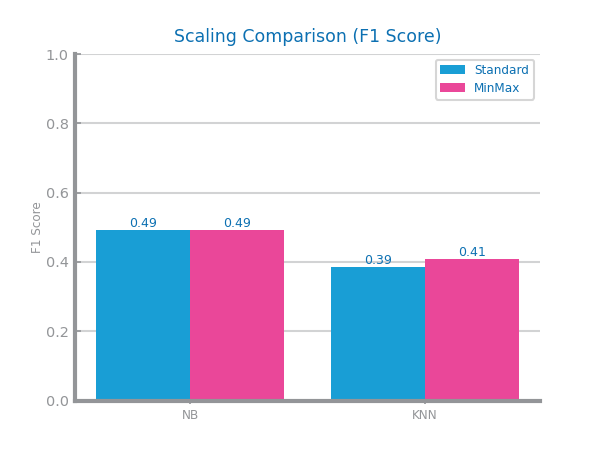
\includegraphics[width=0.9\textwidth]{4_scaling_comparison.png}
\caption{Scaling results with different approaches for dataset 2}
\end{figure}

\subsection*{\textit{Balancing}}
\ctext[RGB]{190,190,190}{Shall contain all relevant information and charts respecting to balancing transformation, such as the choices made and the impact of the different approaches on modelling results. Shall also clearly reveal the approach selected to proceed with the processing. If not applied explain the reason for that, based on data characteristics.  \textbf{Shall not exceed 500 characters.}}

\begin{figure}[H]
\centering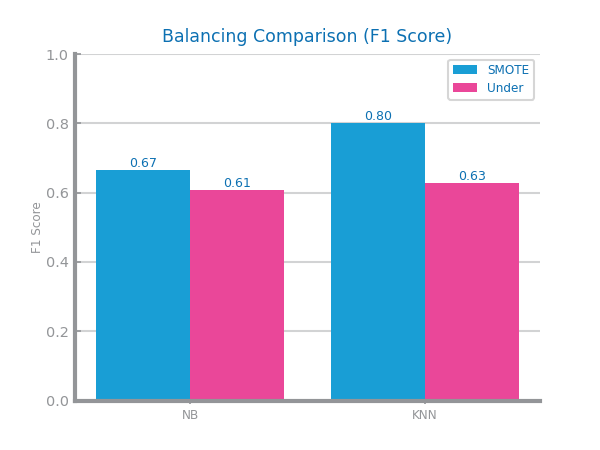
\includegraphics[width=0.9\textwidth]{5_balancing_comparison.png}
\caption{Balancing results with different approaches for dataset 1}
\end{figure}

\begin{figure}[H]
\centering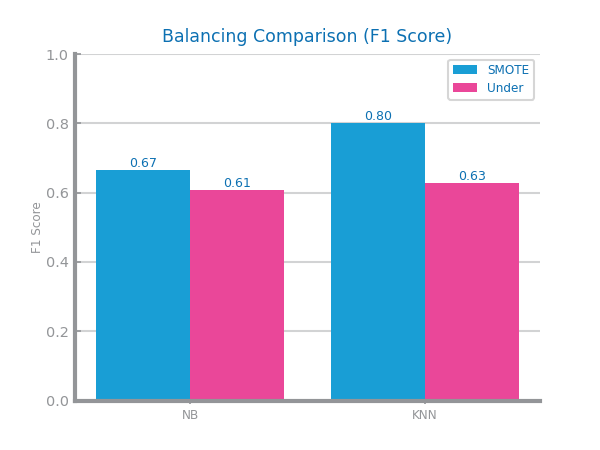
\includegraphics[width=0.9\textwidth]{5_balancing_comparison.png}
\caption{Balancing results with different approaches for dataset 2}
\end{figure}

\subsection*{\textit{Feature Selection}}
\ctext[RGB]{190,190,190}{Shall contain all relevant information and charts respecting to feature selection based on filtering out redundant (based on correlation) and relevant (based on variation) variables. The different choices and their impact on the modelling results shall be presented and explained. Should also clearly reveal the approach selected to proceed with the processing. All explanations shall be based on data characteristics.  \textbf{Shall not exceed 500 characters.}}

\begin{figure}[H]
\centering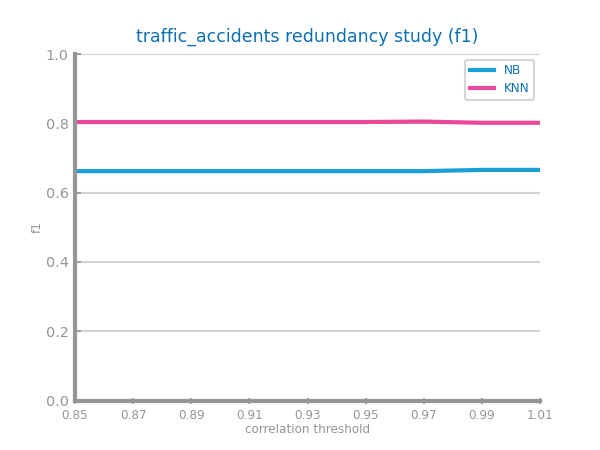
\includegraphics[width=0.9\textwidth]{6_selection_redundancy_f1.png}
\caption{Feature selection of redundant variables results with different parameters for dataset 1}
\end{figure}

\begin{figure}[H]
\centering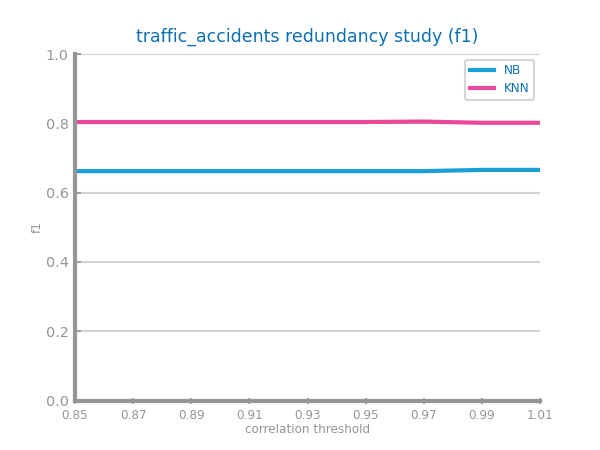
\includegraphics[width=0.9\textwidth]{6_selection_redundancy_f1.png}
\caption{Feature selection of redundant variables results with different parameters for dataset 2}
\end{figure}

\begin{figure}[H]
\centering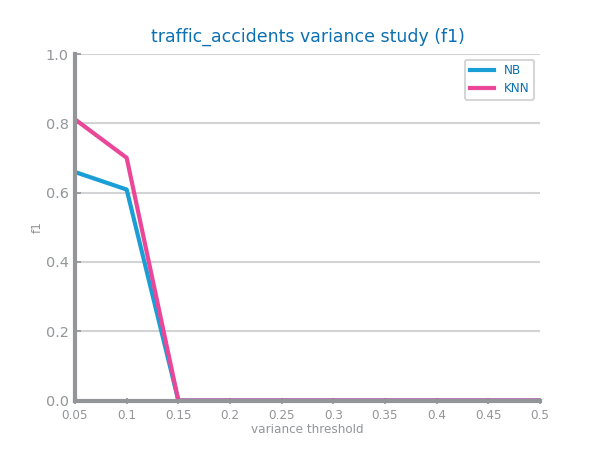
\includegraphics[width=0.9\textwidth]{6_selection_variance_f1.png}
\caption{Feature selection of relevant variables results with different parameters for dataset 1 (variance study)} 
\end{figure}

\begin{figure}[H]
\centering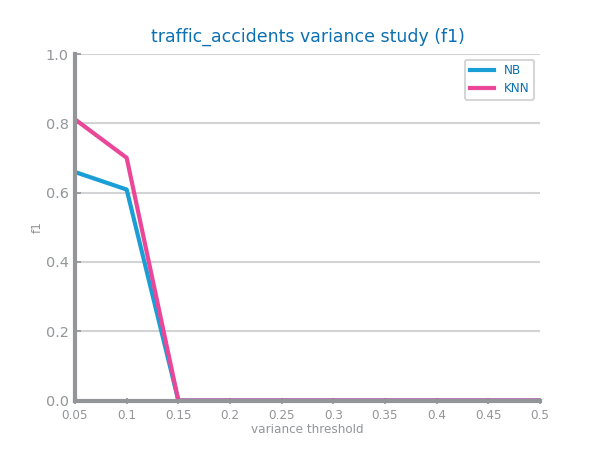
\includegraphics[width=0.9\textwidth]{6_selection_variance_f1.png}
\caption{Feature selection of relevant variables results with different parameters for dataset 2 (variance study)}
\end{figure}

\subsection*{\textit{Feature Extraction (optional)}}
\ctext[RGB]{190,190,190}{Shall contain all relevant information and charts respecting to feature extraction, in particular PCA. The different choices and their impact on the modelling results shall be presented and explained.  \textbf{Shall not exceed 200 characters.}}

\begin{figure}[H]
%\centering\includegraphics[width=0.9\textwidth]{}
\caption{Principal components analysis and feature extraction results for dataset 1}
\end{figure}

\begin{figure}[H]
%\centering\includegraphics[width=0.9\textwidth]{}
\caption{Principal components analysis and feature extraction results for dataset 2}
\end{figure}

\subsection*{\textit{Additional Feature Generation (if done)}}
\ctext[RGB]{190,190,190}{Shall contain all relevant information and charts respecting to feature generation. The different choices and their impact on the modelling results shall be presented and explained. Shall summarise all variables generated and the formula used to derive them (in a table).  \textbf{Shall not exceed 200 characters.}}

\begin{figure}[H]
%\centering\includegraphics[width=0.9\textwidth]{}
\caption{Feature generation results for dataset 1}
\end{figure}

\begin{figure}[H]
%\centering\includegraphics[width=0.9\textwidth]{}
\caption{Feature generation results for dataset 2}
\end{figure}

\section{MODELS' EVALUATION}
\ctext[RGB]{190,190,190}{Shall be used to point out any important decision taken during the training, including training strategy and evaluation measures used.  \textbf{Shall not exceed 500 characters.}}

\subsection*{\textit{Na{\"i}ve Bayes}}
\ctext[RGB]{190,190,190}{Shall be used to present the results achieved with each one of Na{\"i}ve Bayes implementations, comparing and proposing explanations for them. If any of the implementations is not used, a justification for it shall be presented. Shall be used to present the evaluation of the best model achieved.  \textbf{Shall not exceed 300 characters.}}

\begin{figure}[H]
\centering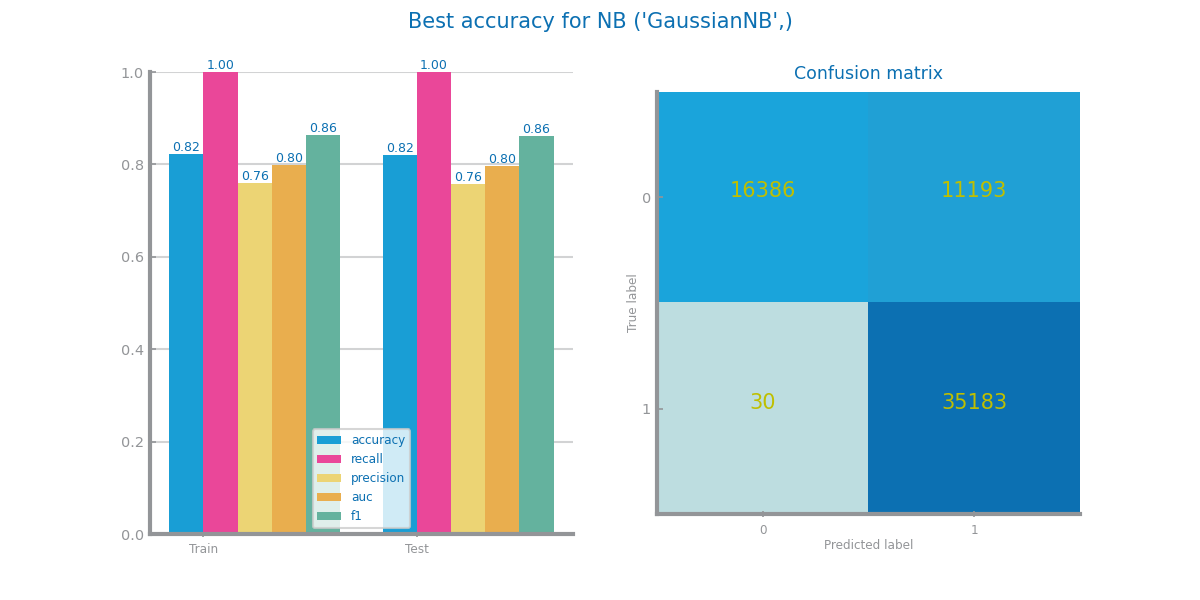
\includegraphics[width=0.9\textwidth]{accidents_nb_NB_best_accuracy_eval.png}
\caption{Na{\"i}ve Bayes alternatives comparison for dataset 1}
\end{figure}

\begin{figure}[H]
\centering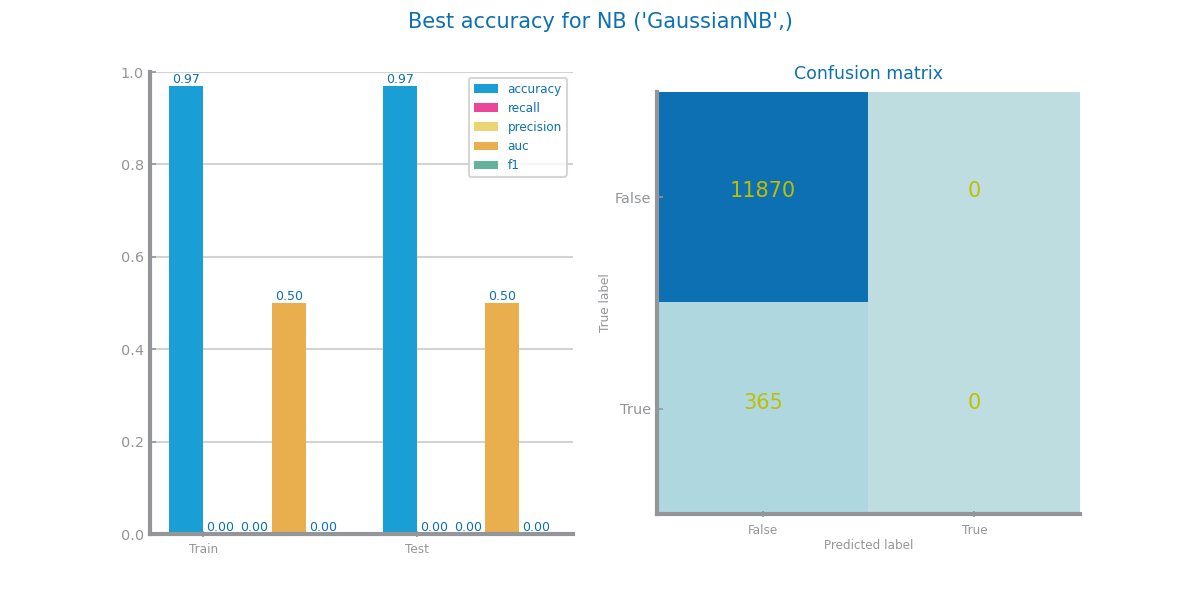
\includegraphics[width=0.9\textwidth]{flights_nb_NB_best_accuracy_eval.png}
\caption{Na{\"i}ve Bayes alternative comparison for dataset 2}
\end{figure}

\begin{figure}[H]
    \centering
    \begin{subfigure}[b]{0.45\textwidth}
        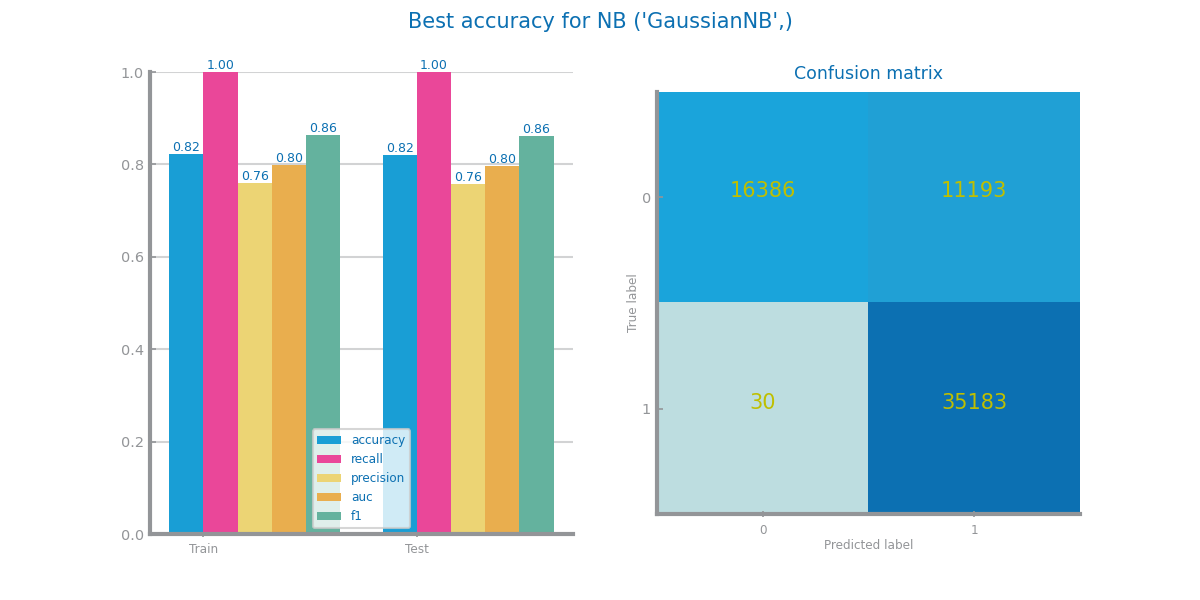
\includegraphics[width=\textwidth]{accidents_nb_NB_best_accuracy_eval.png}
    \end{subfigure}
    \hfill
    \begin{subfigure}[b]{0.45\textwidth}
        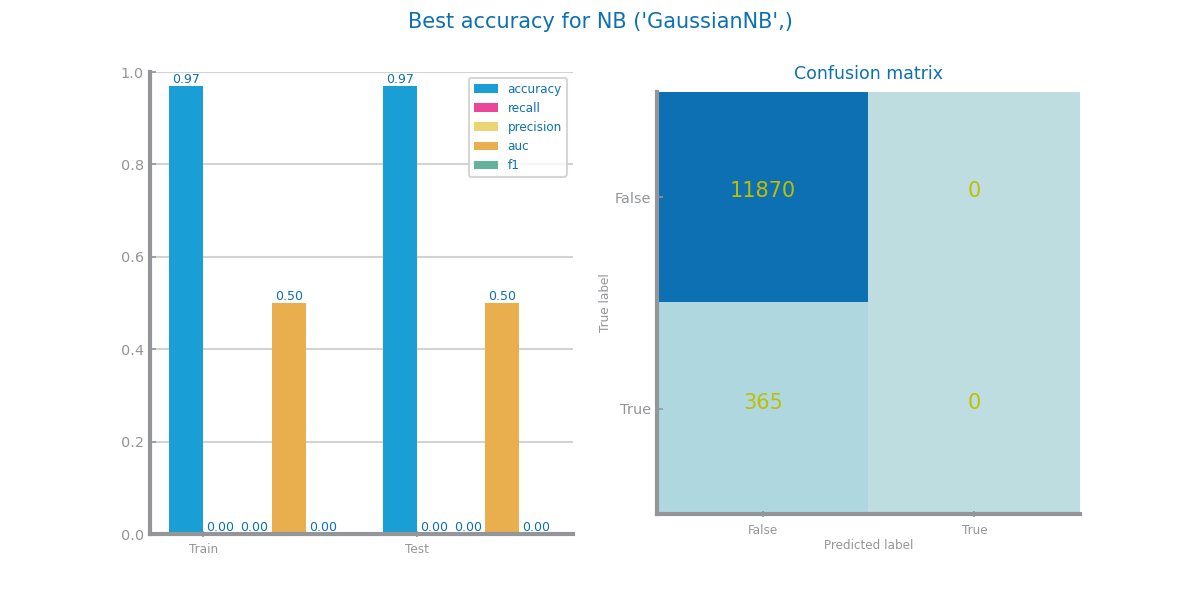
\includegraphics[width=\textwidth]{flights_nb_NB_best_acuracy_eval.png}
    \end{subfigure}
    \caption{Na{\"i}ve Bayes best model results for dataset 1 (left) and dataset 2 (right)}
\end{figure}

\subsection*{\textit{KNN}}
\ctext[RGB]{190,190,190}{Shall be used to present the results achieved through different similarity measures and KNN parameterisations. The results shall be compared and explanations for them shall be presented. The justification for the chosen similarity measures shall be presented. Shall be used to address the overfitting phenomenon, studying the conditions under which models face it. Shall be used to present the evaluation of the best model achieved.  \textbf{Shall not exceed 500 characters.}}

\begin{figure}[H]
\centering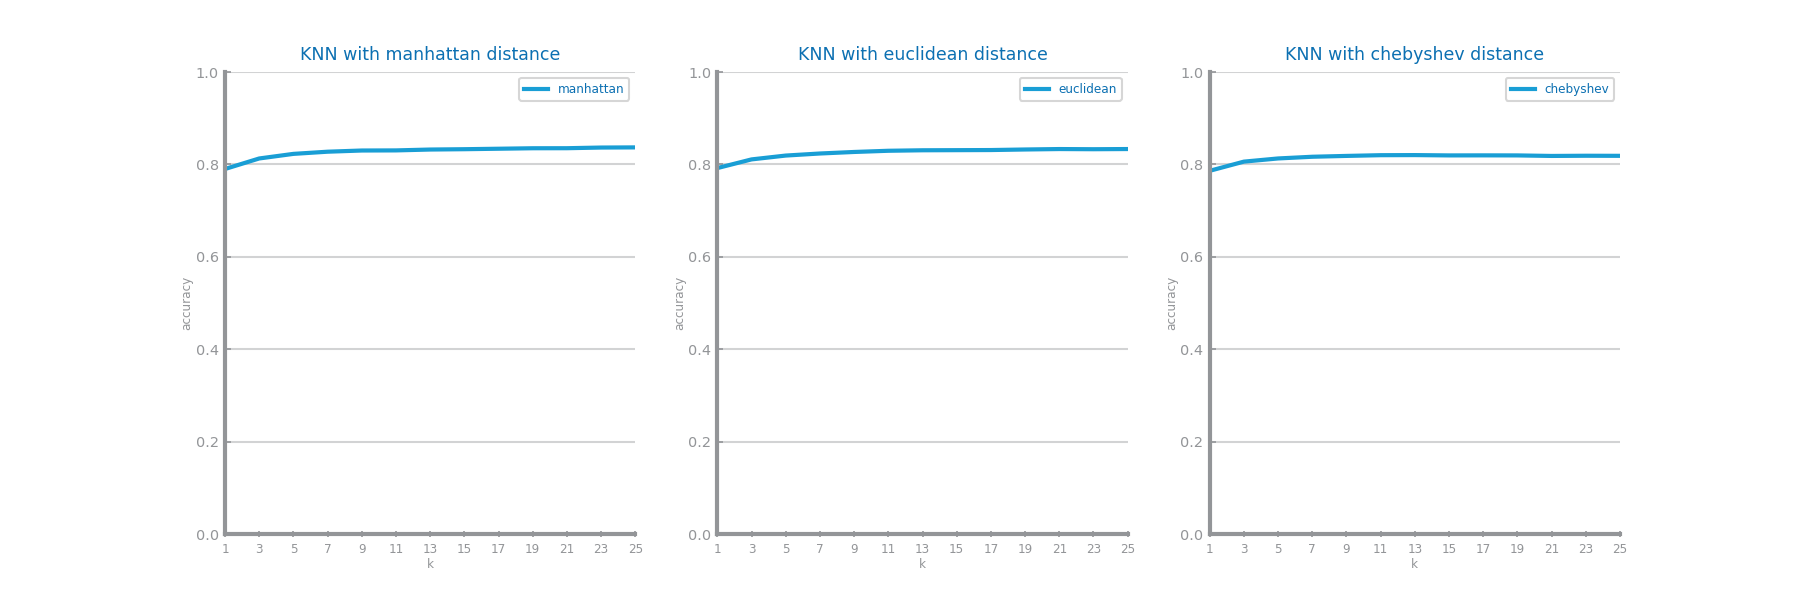
\includegraphics[width=0.9\textwidth]{accidents_knn_accuracy_study.png}
\caption{KNN different parameterisations comparison for dataset 1}
\end{figure}

\begin{figure}[H]
\centering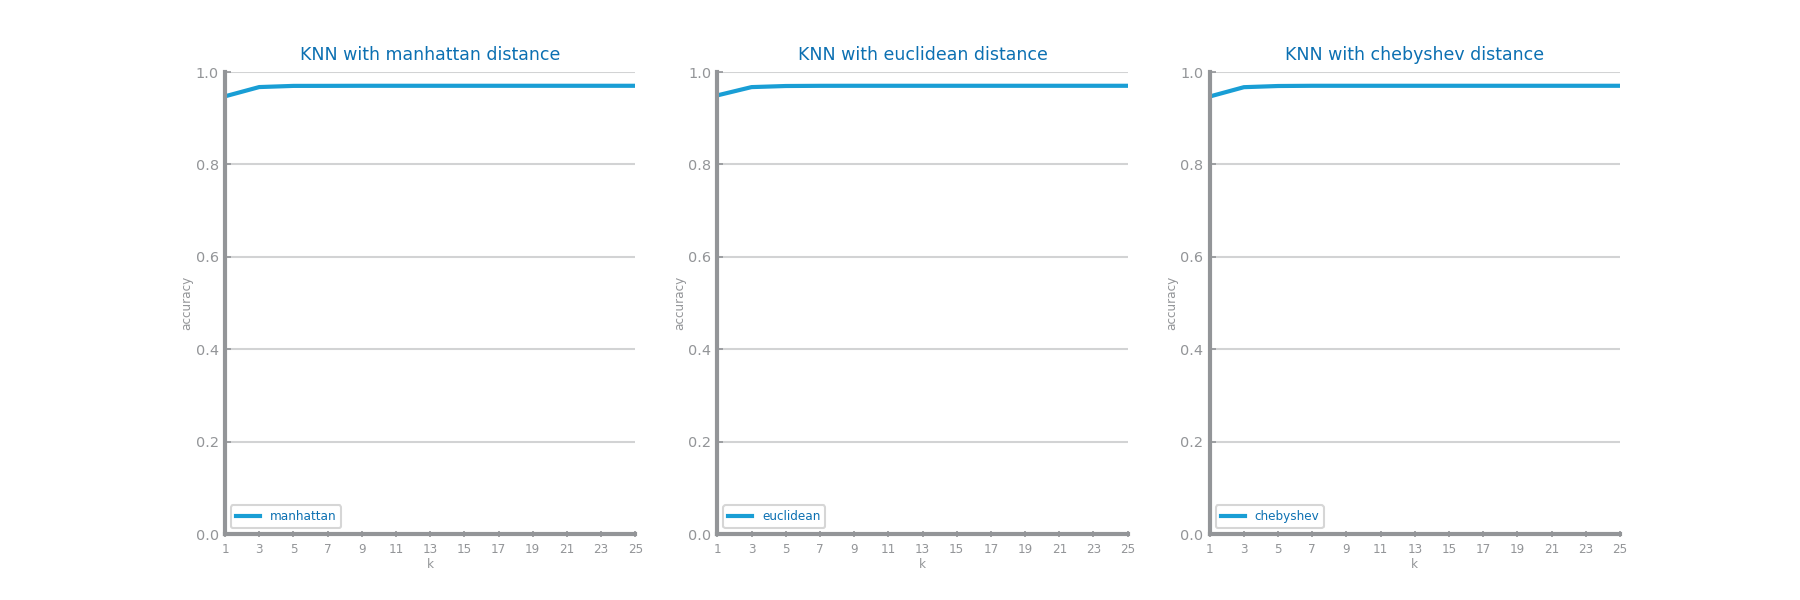
\includegraphics[width=0.9\textwidth]{flights_knn_accuracy_study.png}
\caption{KNN different parameterisations comparison for dataset 2}
\end{figure}

\begin{figure}[H]
    \centering
    \begin{subfigure}[b]{0.45\textwidth}
        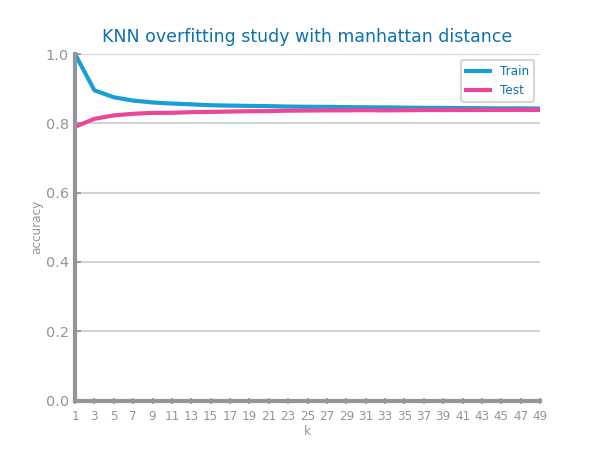
\includegraphics[width=\textwidth]{accidents_knn_accuracy_overfitting.png}
    \end{subfigure}
    \hfill
    \begin{subfigure}[b]{0.45\textwidth}
        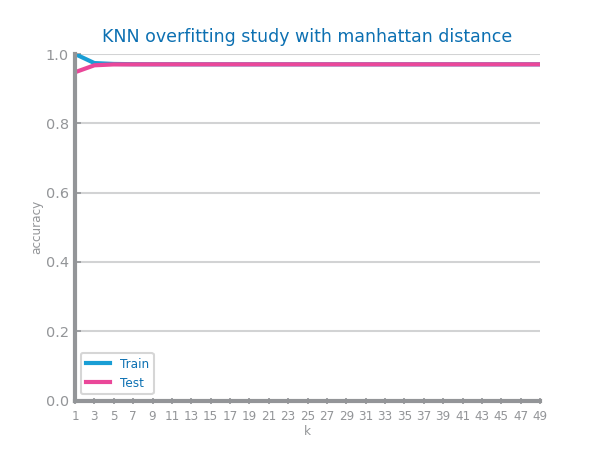
\includegraphics[width=\textwidth]{flights_knn_accuracy_overfitting.png}
    \end{subfigure}
    \caption{KNN overfitting analysis for dataset 1 (left) and dataset 2 (right)}
\end{figure}

\begin{figure}[H]
    \centering
    \begin{subfigure}[b]{0.45\textwidth}
        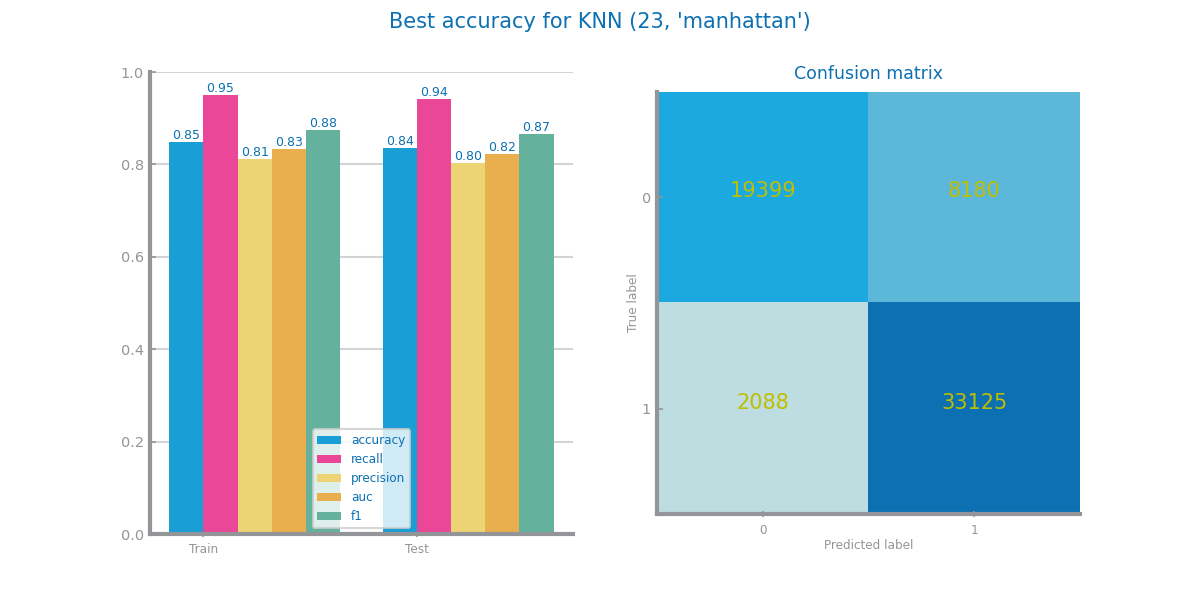
\includegraphics[width=\textwidth]{accidents_knn_KNN_best_accuracy_eval.png}
    \end{subfigure}
    \hfill
    \begin{subfigure}[b]{0.45\textwidth}
        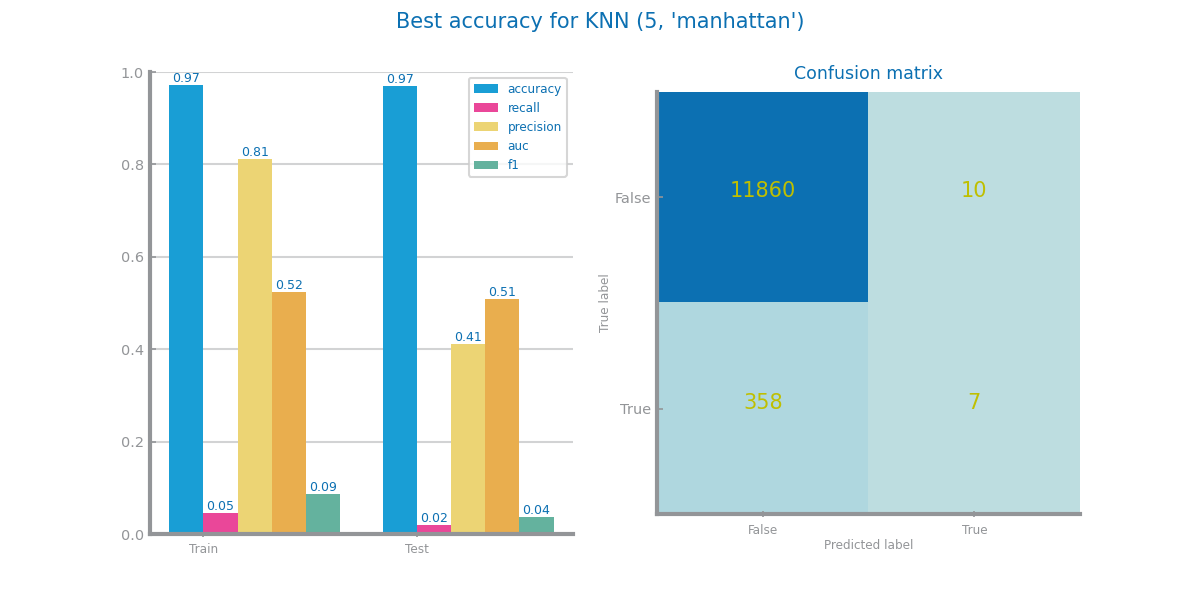
\includegraphics[width=\textwidth]{flights_knn_KNN_best_accuracy_eval.png}
    \end{subfigure}
    \caption{KNN best model results for dataset 1 (left) and dataset 2 (right)}
\end{figure}

\subsection*{\textit{Decision Trees}}
\ctext[RGB]{190,190,190}{Shall be used to present the results achieved through different parameterisations for the train of decision trees. The results shall be compared and explanations for them shall be presented. Shall be used to address the overfitting phenomenon, studying the conditions under which models face it. Shall be used to present the evaluation of the best model achieved. Shall be used to present the best tree achieved and its succinct description.  \textbf{Shall not exceed 500 characters.}}

\begin{figure}[H]
\centering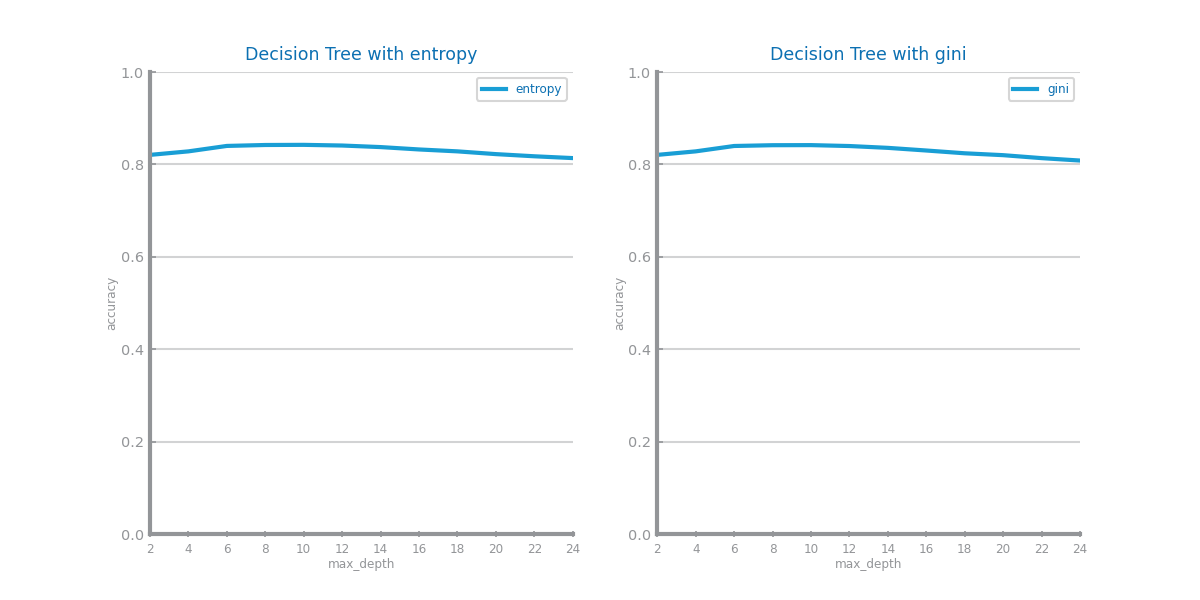
\includegraphics[width=0.9\textwidth]{accidents_dt_accuracy_study.png}
\caption{Decision Trees different parameterisations comparison for dataset 1}
\end{figure}

\begin{figure}[H]
\centering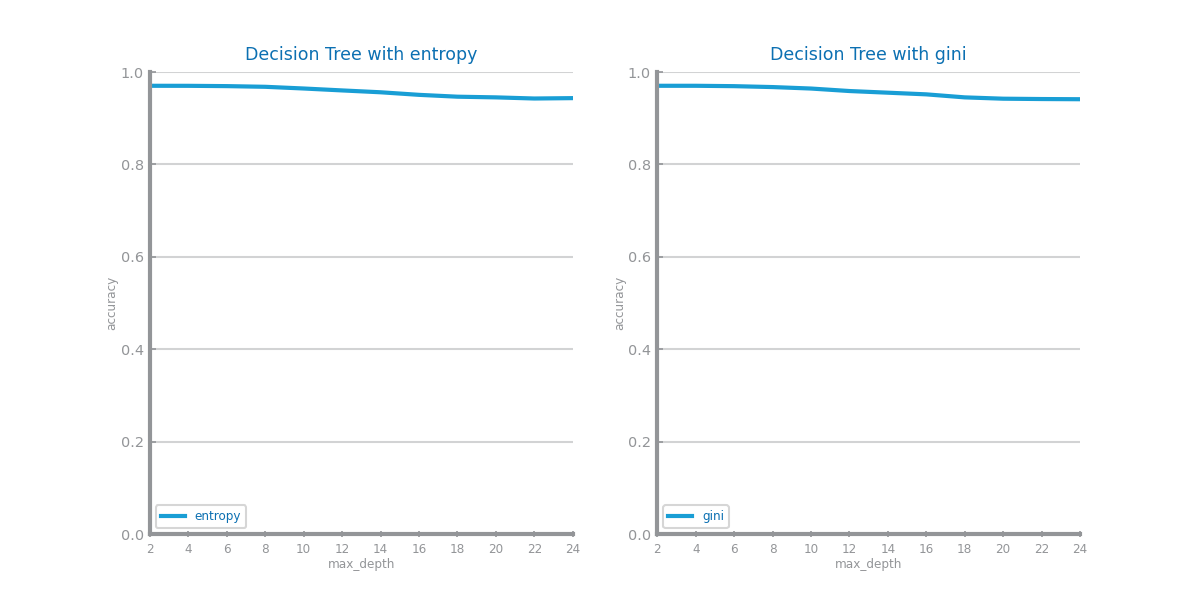
\includegraphics[width=0.9\textwidth]{flights_dt_accuracy_study.png}
\caption{Decision Trees different parameterisations comparison for dataset 2}
\end{figure}

\begin{figure}[H]
    \centering
    \begin{subfigure}[b]{0.45\textwidth}
        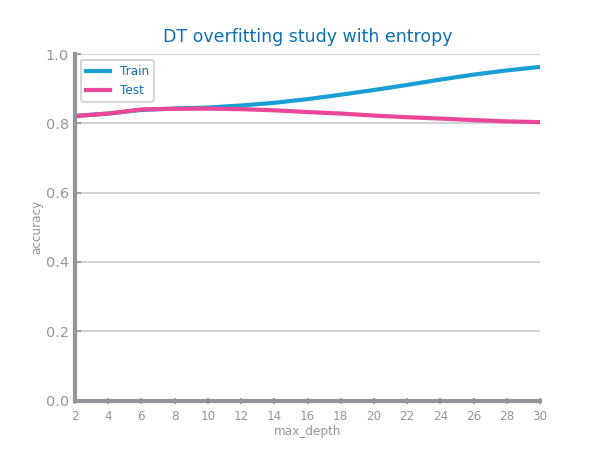
\includegraphics[width=\textwidth]{accidents_dt_accuracy_overfitting.png}
    \end{subfigure}
    \hfill
    \begin{subfigure}[b]{0.45\textwidth}
        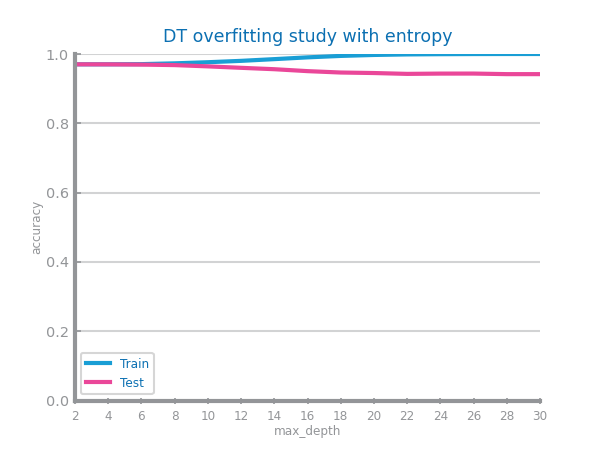
\includegraphics[width=\textwidth]{flights_dt_accuracy_overfitting.png}
    \end{subfigure}
    \caption{Decision Trees overfitting analysis for dataset 1 (left) and dataset 2 (right)}
\end{figure}

\begin{figure}[H]
    \centering
    \begin{subfigure}[b]{0.45\textwidth}
        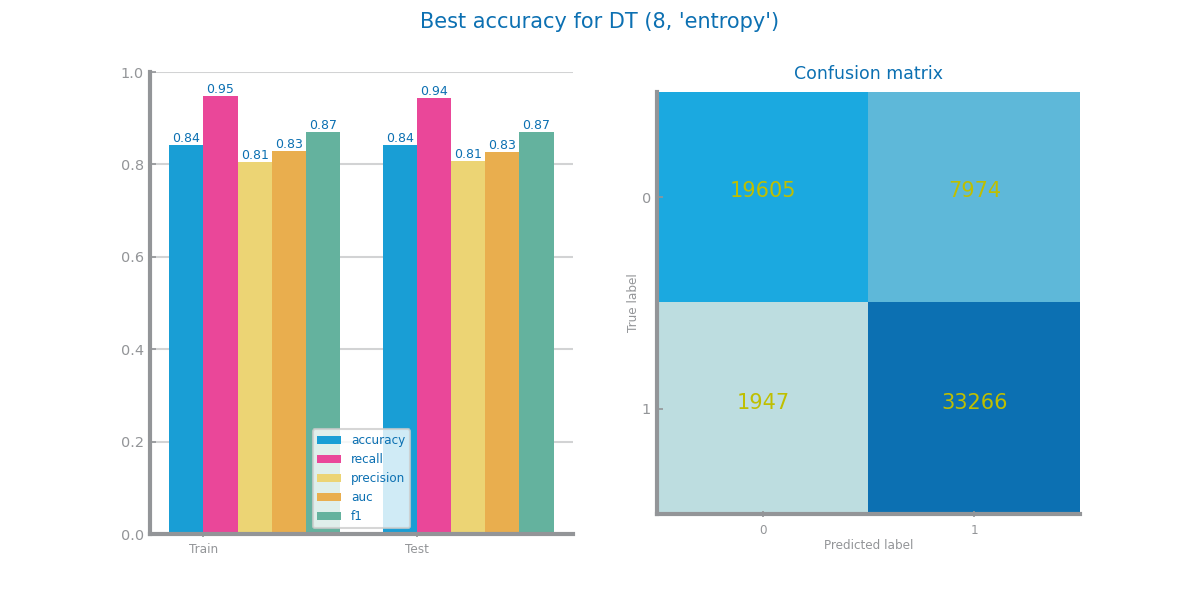
\includegraphics[width=\textwidth]{accidents_dt_DT_best_accuracy_eval.png}
    \end{subfigure}
    \hfill
    \begin{subfigure}[b]{0.45\textwidth}
        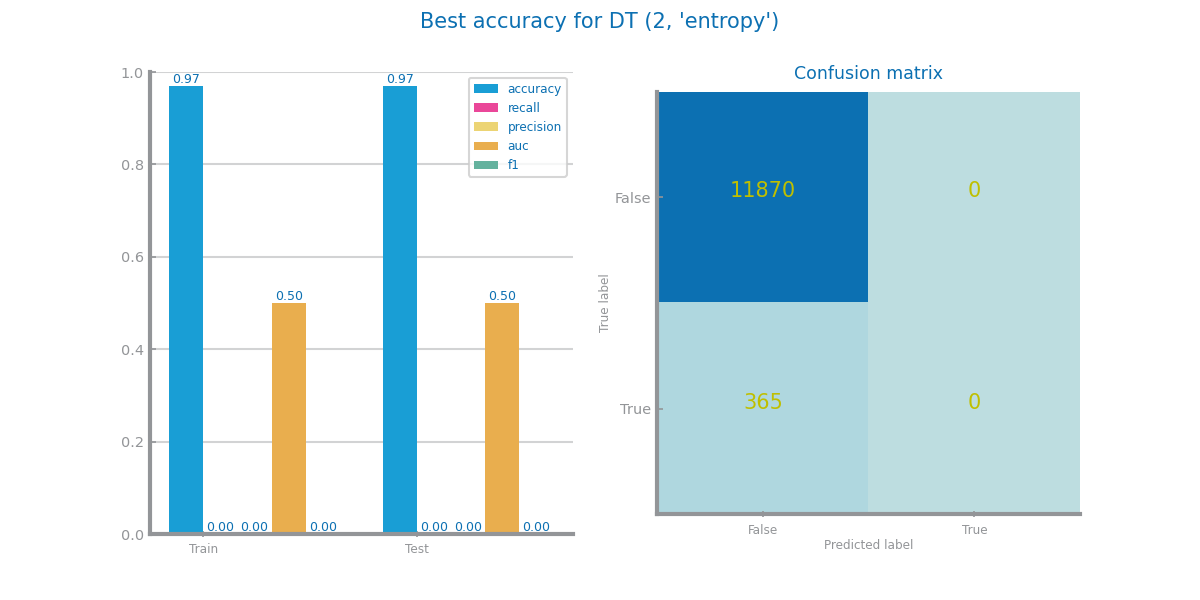
\includegraphics[width=\textwidth]{flights_dt_DT_best_accuracy_eval.png}
    \end{subfigure}
    \caption{Decision trees best model results for dataset 1 (left) and dataset 2 (right)}
\end{figure}

\begin{figure}[H]
\centering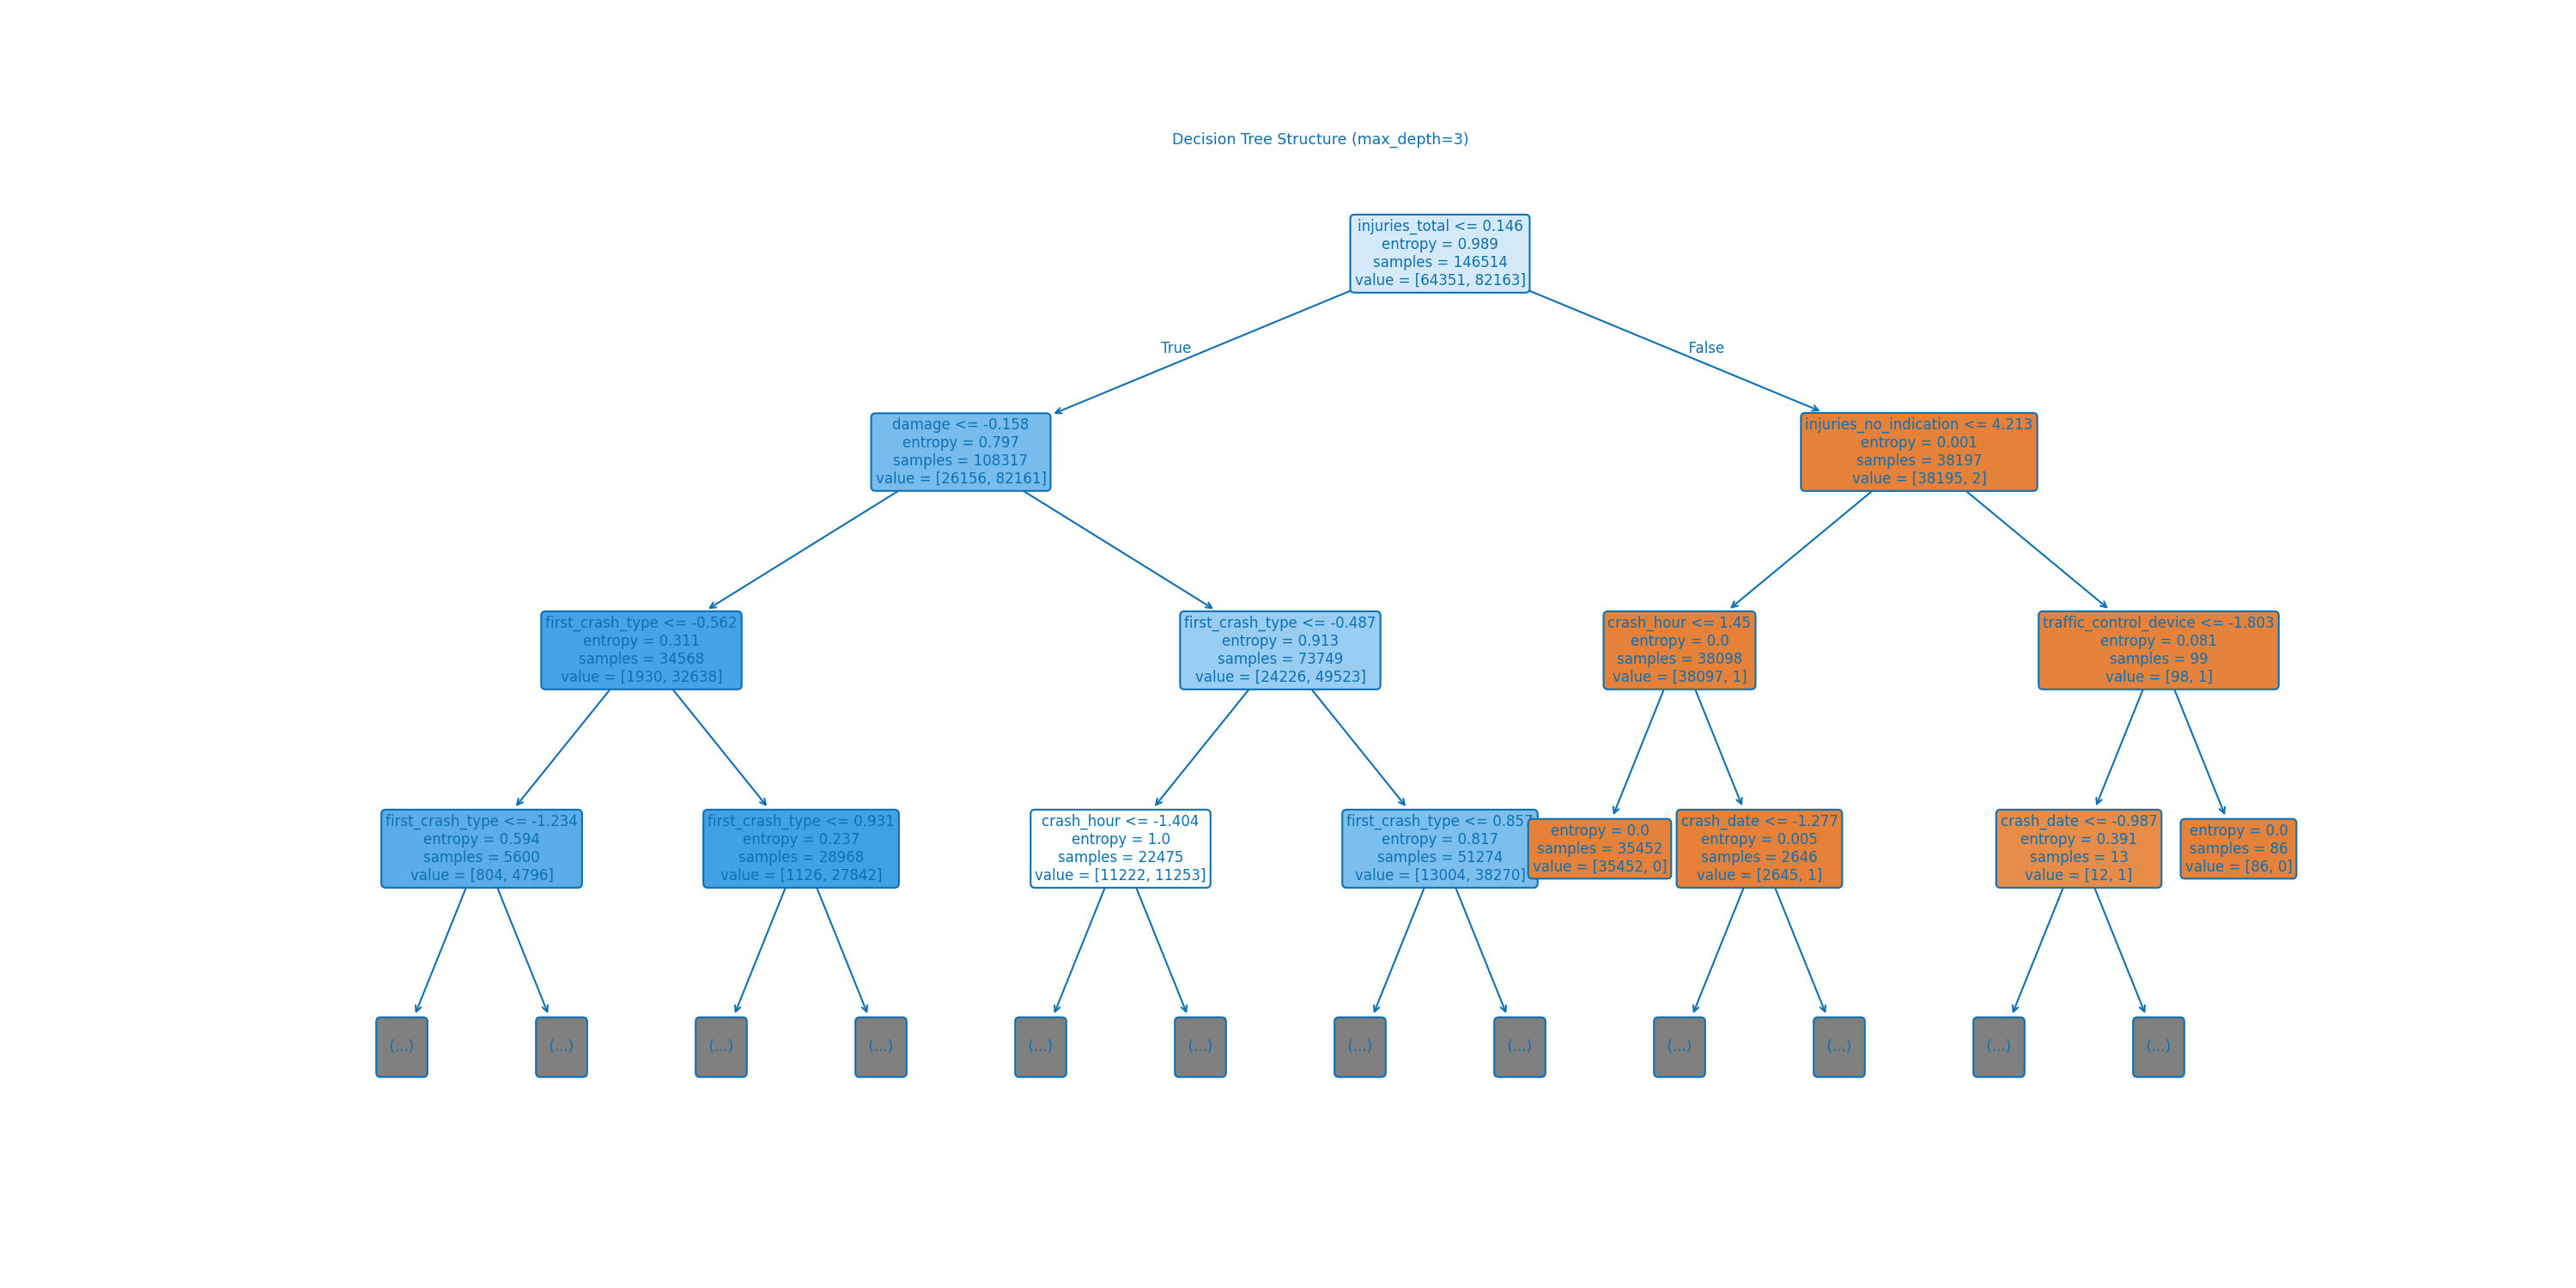
\includegraphics[width=0.9\textwidth]{accidents_dt_tree.png}
\caption{Best tree for dataset 1}
\end{figure}

\begin{figure}[H]
\centering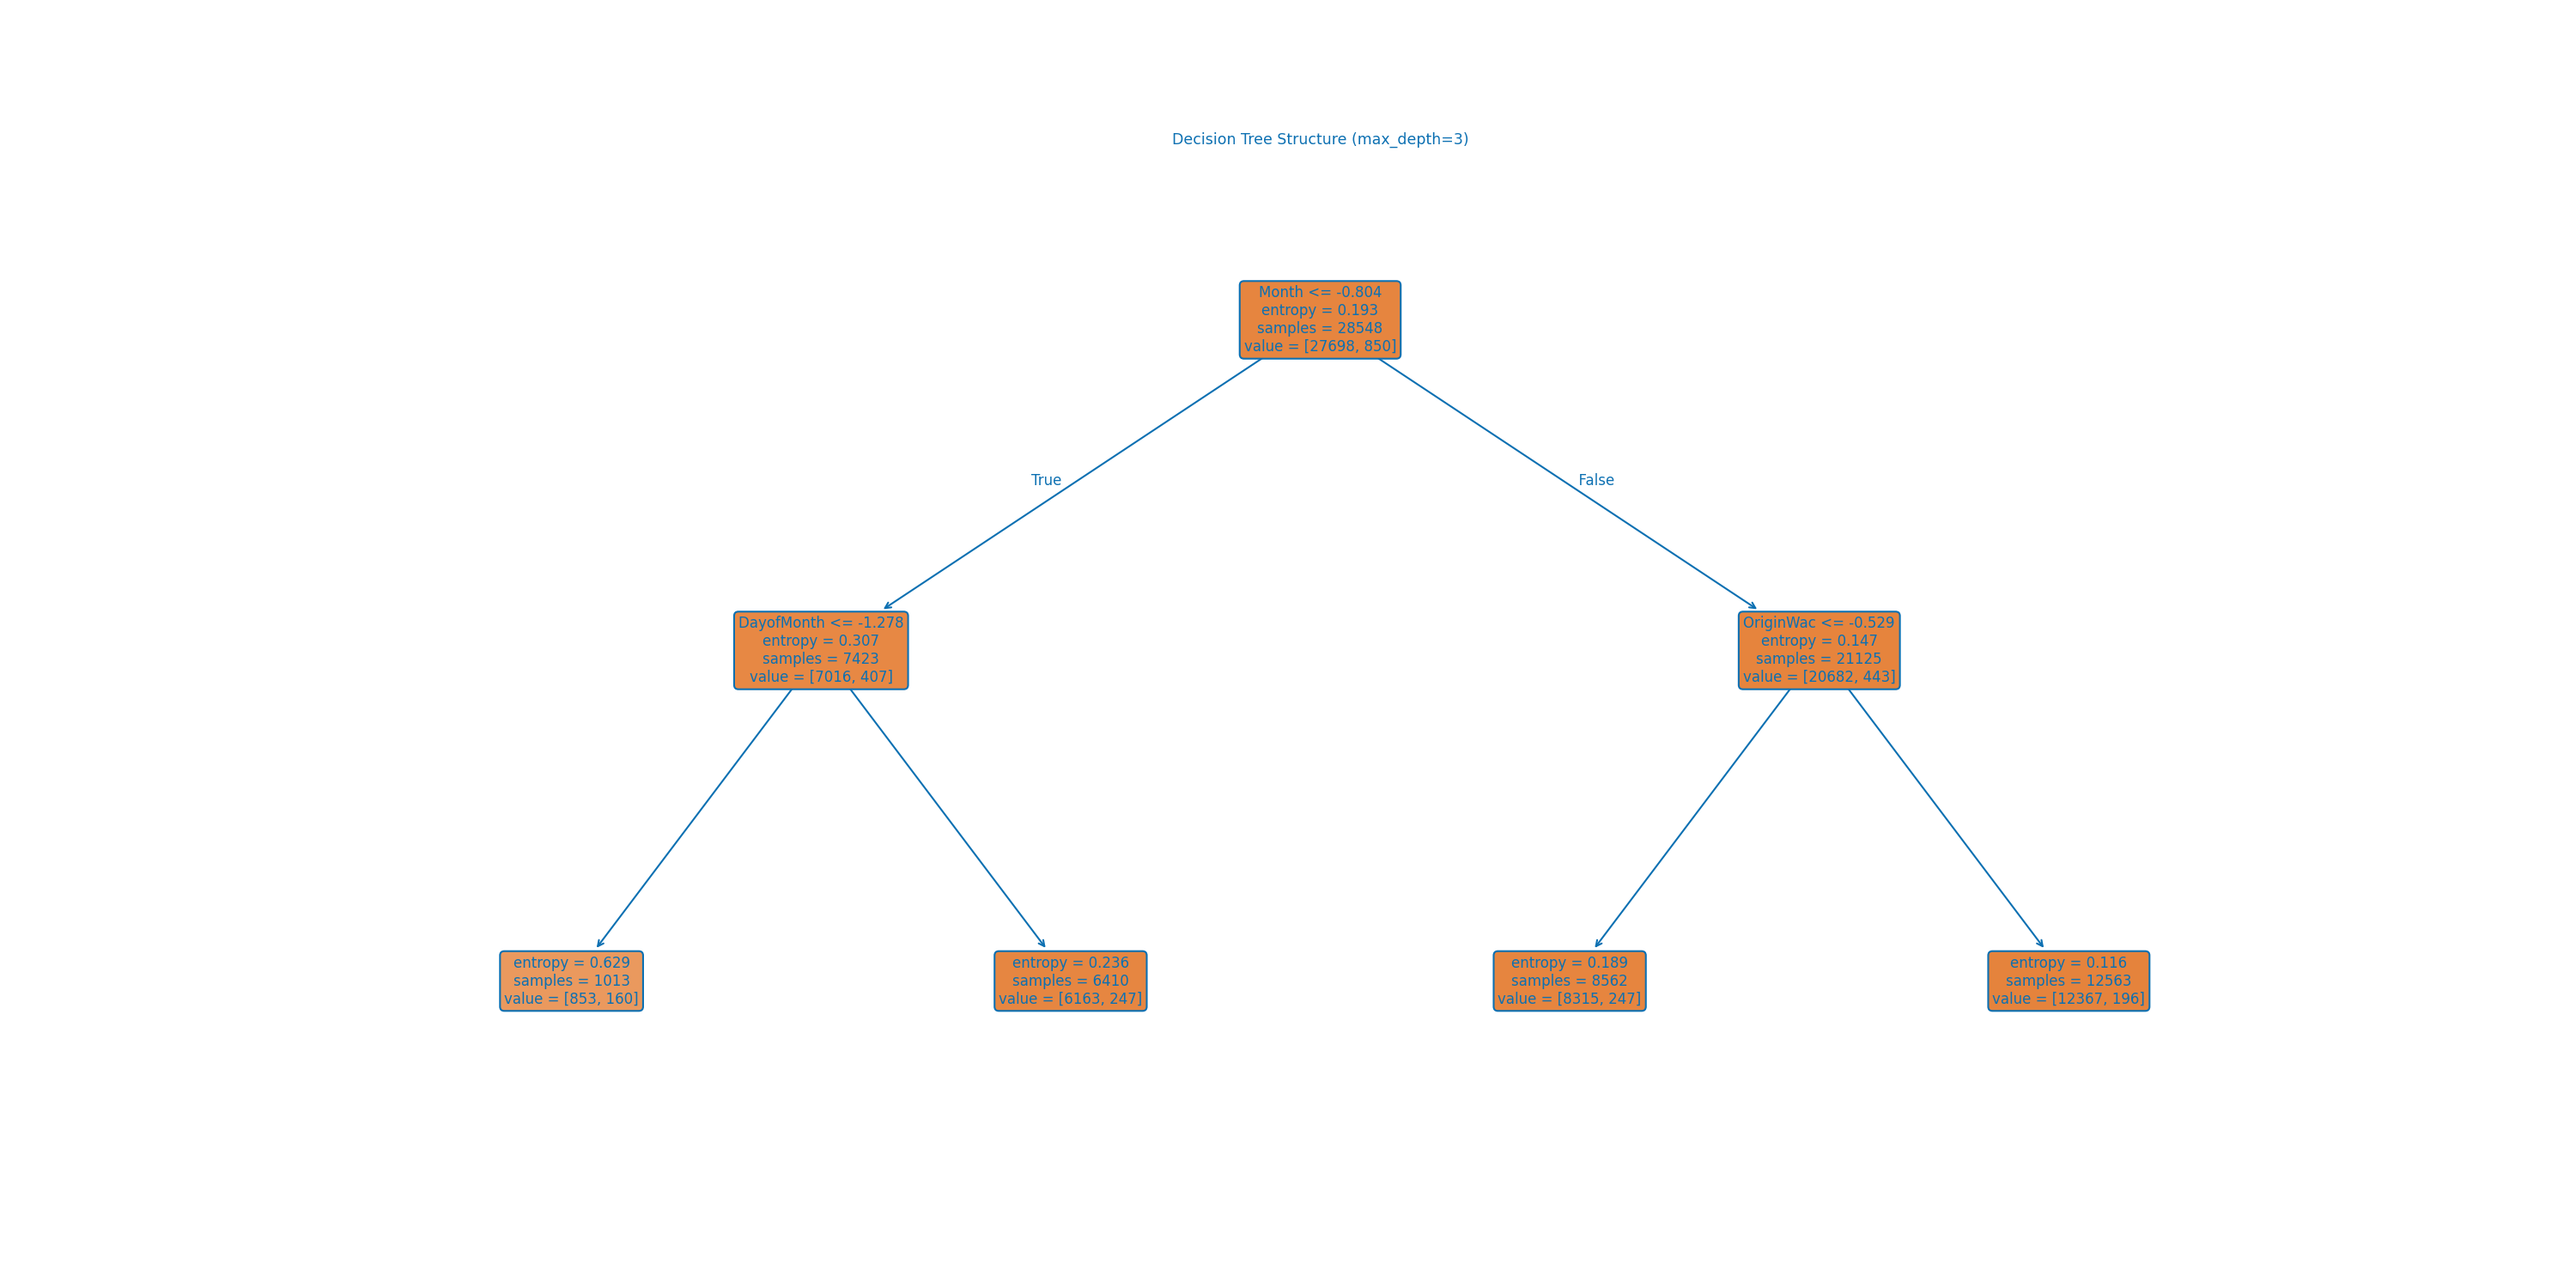
\includegraphics[width=0.9\textwidth]{flights_dt_tree.png}
\caption{Best tree for dataset 2}
\end{figure}

\subsection*{\textit{Random Forests}}
\ctext[RGB]{190,190,190}{Shall be used to present the results achieved through different parameterisations for the train of random forests. The results shall be compared and explanations for them shall be presented. Shall be used to address the overfitting phenomenon, studying the conditions under which models face it. Shall be used to present the evaluation of the best model achieved. May be used to present the most important variables in the model.  \textbf{Shall not exceed 500 characters.}}

\begin{figure}[H]
\centering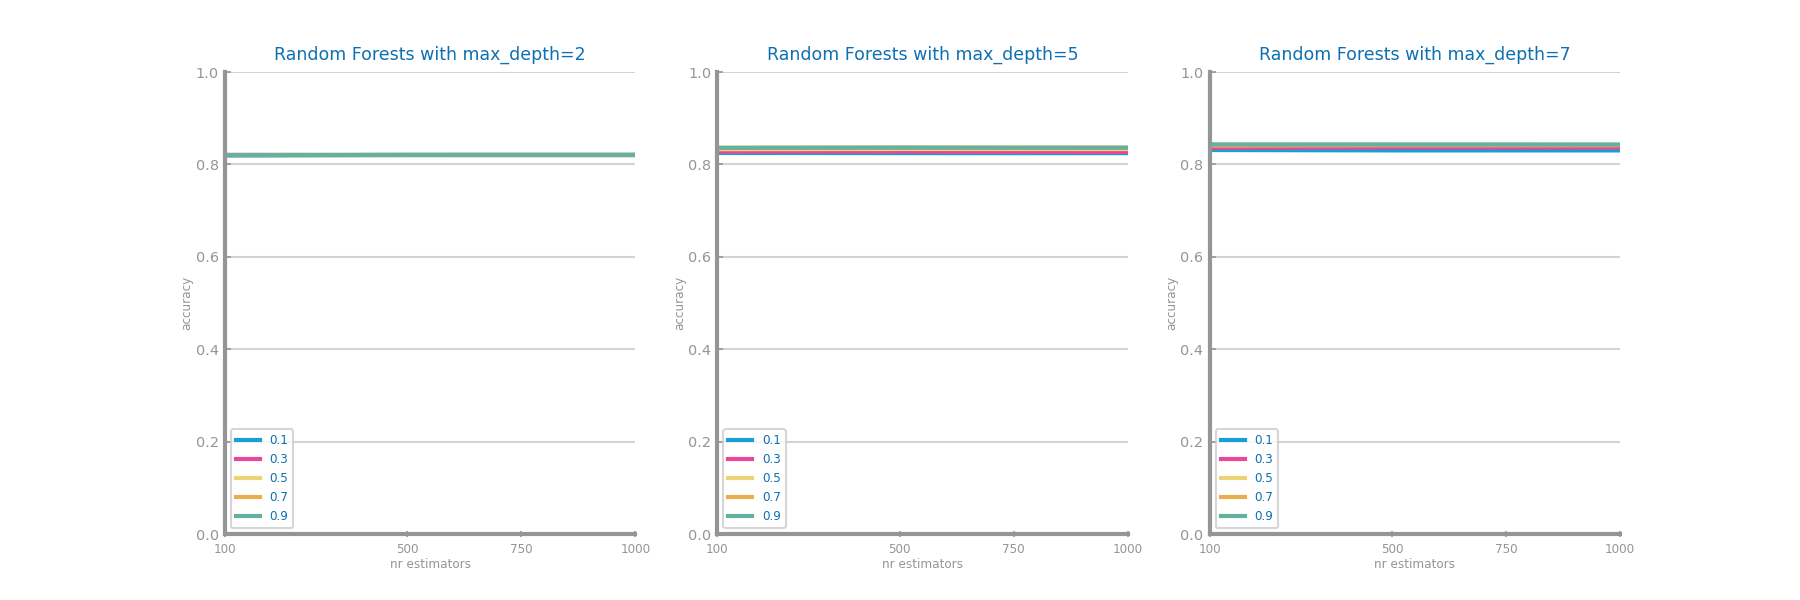
\includegraphics[width=0.9\textwidth]{accidents_rf_accuracy_study.png}
\caption{Random Forests different parameterisations comparison for dataset 1}
\end{figure}

\begin{figure}[H]
\centering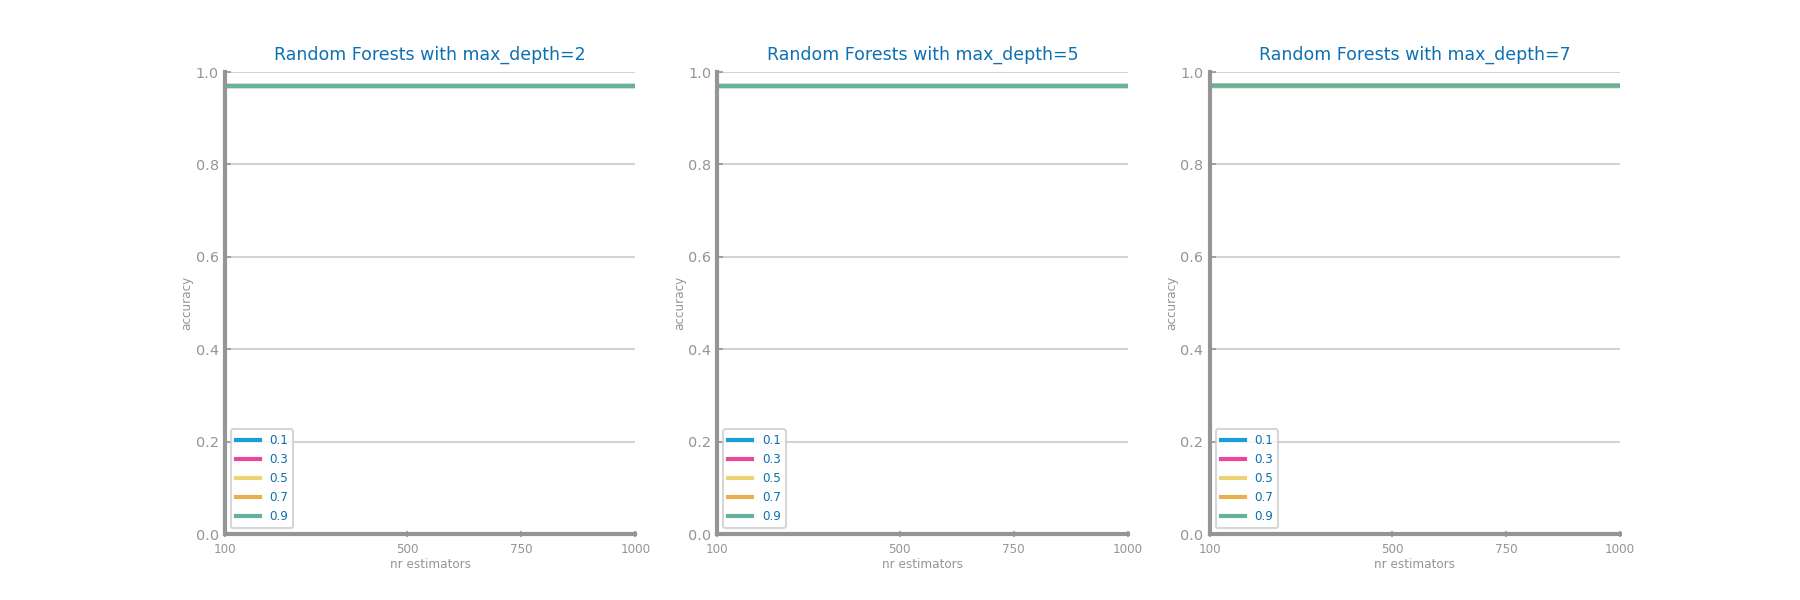
\includegraphics[width=0.9\textwidth]{flights_rf_accuracy_study.png}
\caption{Random Forests different parameterisations comparison for dataset 2}
\end{figure}

\begin{figure}[H]
    \centering
    \begin{subfigure}[b]{0.45\textwidth}
        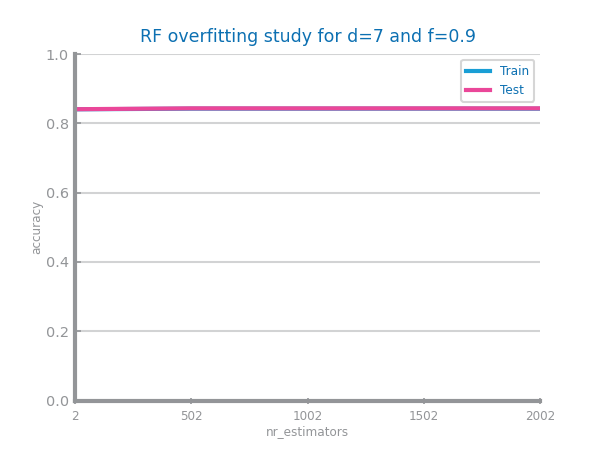
\includegraphics[width=\textwidth]{accidents_rf_accuracy_overfitting.png}
    \end{subfigure}
    \hfill
    \begin{subfigure}[b]{0.45\textwidth}
        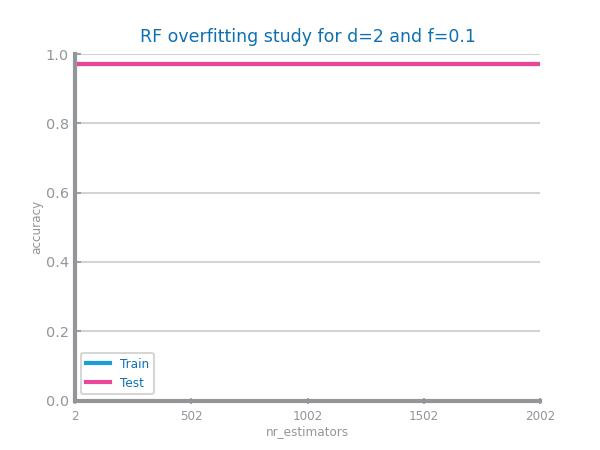
\includegraphics[width=\textwidth]{flights_rf_accuracy_overfitting.png}
    \end{subfigure}
    \caption{Random Forests overfitting analysis for dataset 1 (left) and dataset 2 (right)}
\end{figure}

\begin{figure}[H]
    \centering
    \begin{subfigure}[b]{0.45\textwidth}
        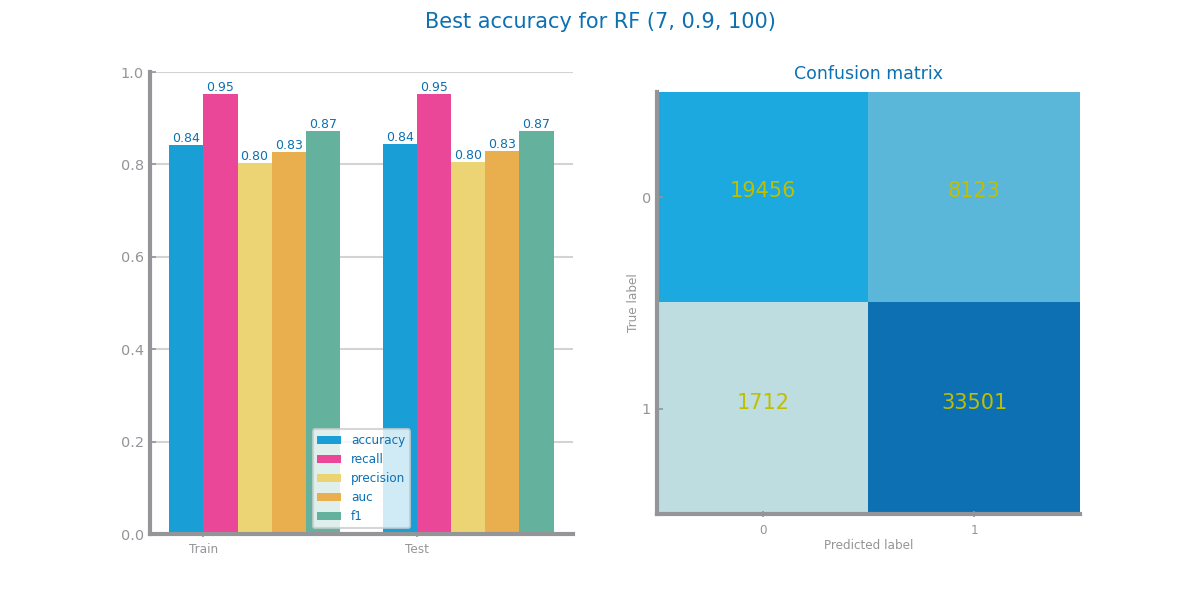
\includegraphics[width=\textwidth]{accidents_rf_RF_best_accuracy_eval.png}
    \end{subfigure}
    \hfill
    \begin{subfigure}[b]{0.45\textwidth}
        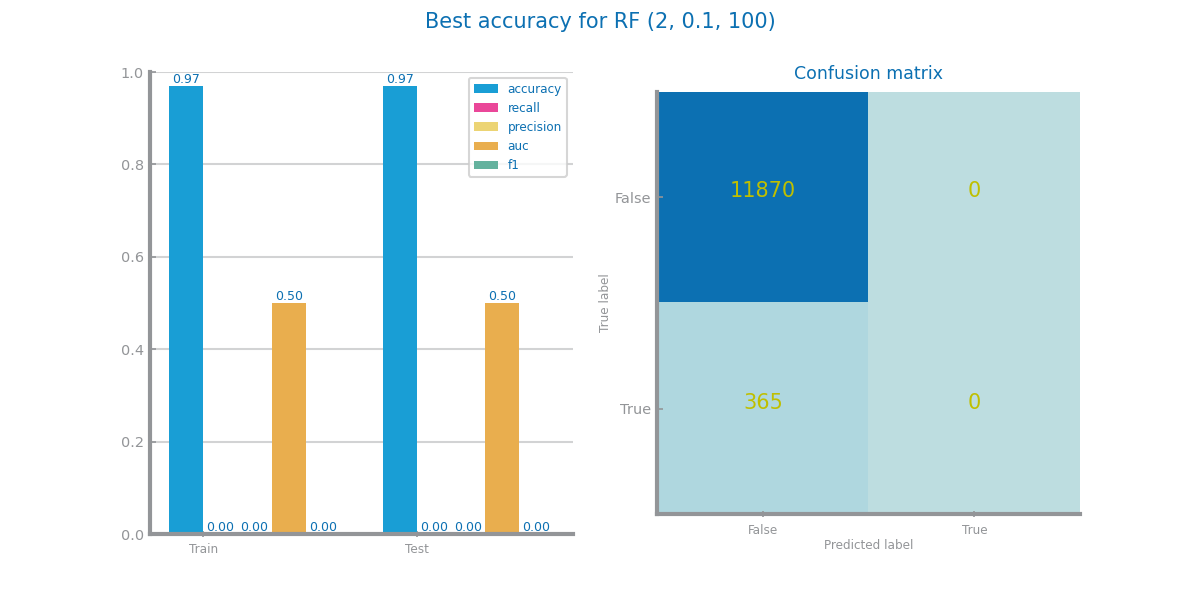
\includegraphics[width=\textwidth]{flights_rf_RF_best_accuracy_eval.png}
    \end{subfigure}
    \caption{Random Forests best model results for dataset 1 (left) and dataset 2 (right)}
\end{figure}

\begin{figure}[H]
    \centering
    \begin{subfigure}[b]{0.45\textwidth}
        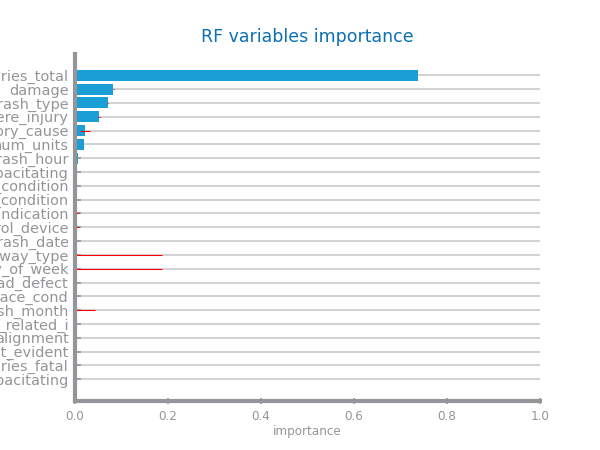
\includegraphics[width=\textwidth]{accidents_rf_accuracy_vars_ranking.png}
    \end{subfigure}
    \hfill
    \begin{subfigure}[b]{0.45\textwidth}
        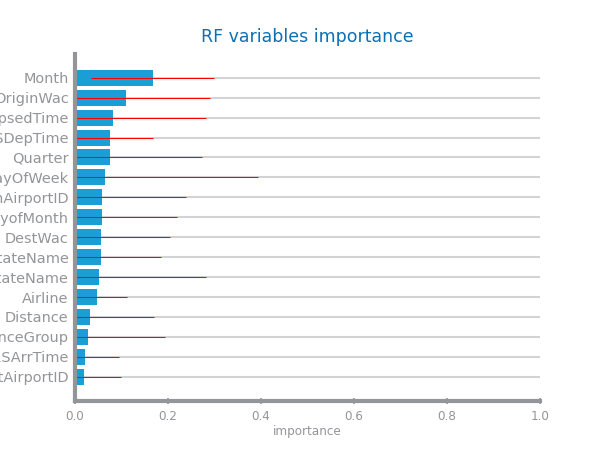
\includegraphics[width=\textwidth]{flights_rf_accuracy_vars_ranking.png}
    \end{subfigure}
    \caption{Random Forests variables importance for dataset 1 (left) and dataset 2 (right)}
\end{figure}

\subsection*{\textit{Gradient Boosting}}
\ctext[RGB]{190,190,190}{Shall be used to present the results achieved through different parameterisations for the train of gradient boosting. The results shall be compared and explanations for them shall be presented. Shall be used to address the overfitting phenomenon, studying the conditions under which models face it.  Shall be used to present the evaluation of the best model achieved. May be used to present the most important variables in the model.  \textbf{Shall not exceed 500 characters.}}

\begin{figure}[H]
\centering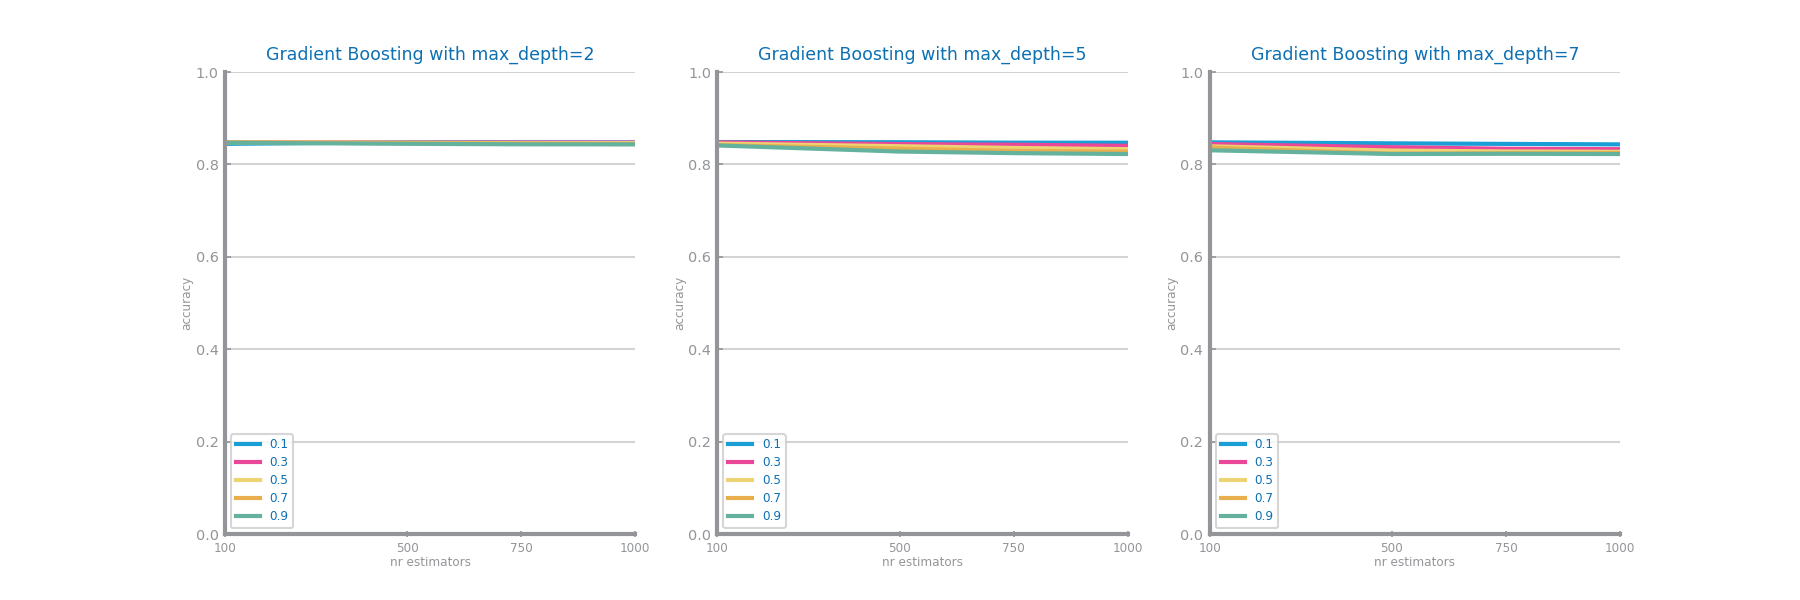
\includegraphics[width=0.9\textwidth]{accidents_gb_accuracy_study.png}
\caption{Gradient boosting different parameterisations comparison for dataset 1}
\end{figure}

\begin{figure}[H]
\centering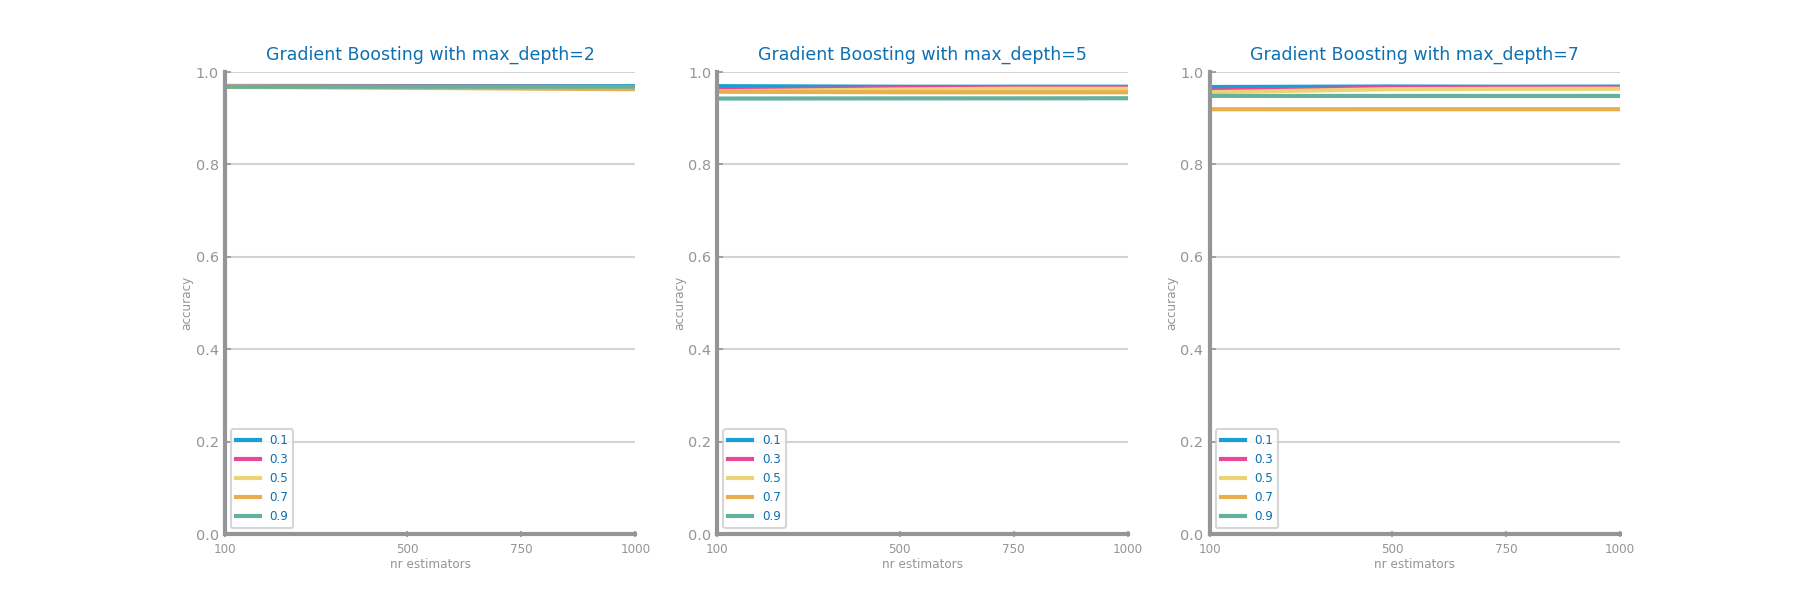
\includegraphics[width=0.9\textwidth]{flights_gb_accuracy_study.png}
\caption{Gradient boosting different parameterisations comparison for dataset 2}
\end{figure}

\begin{figure}[H]
    \centering
    \begin{subfigure}[b]{0.45\textwidth}
        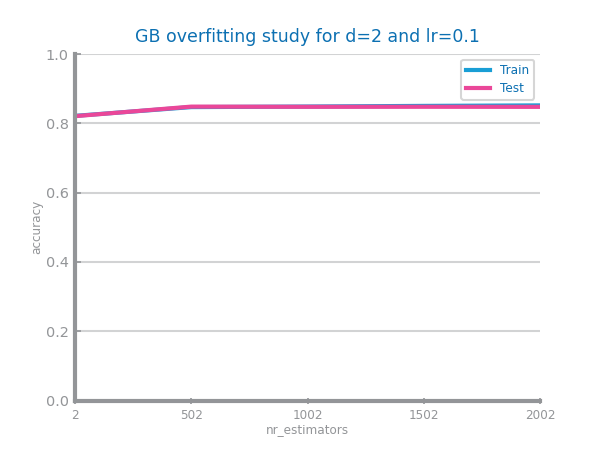
\includegraphics[width=\textwidth]{accidents_gb_accuracy_overfitting.png}
    \end{subfigure}
    \hfill
    \begin{subfigure}[b]{0.45\textwidth}
        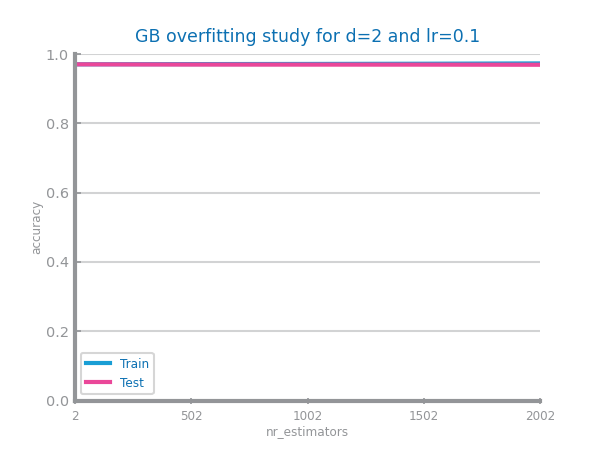
\includegraphics[width=\textwidth]{flights_gb_accuracy_overfitting.png}
    \end{subfigure}
    \caption{Gradient boosting overfitting analysis for dataset 1 (left) and dataset 2 (right)}
\end{figure}

\begin{figure}[H]
    \centering
    \begin{subfigure}[b]{0.45\textwidth}
        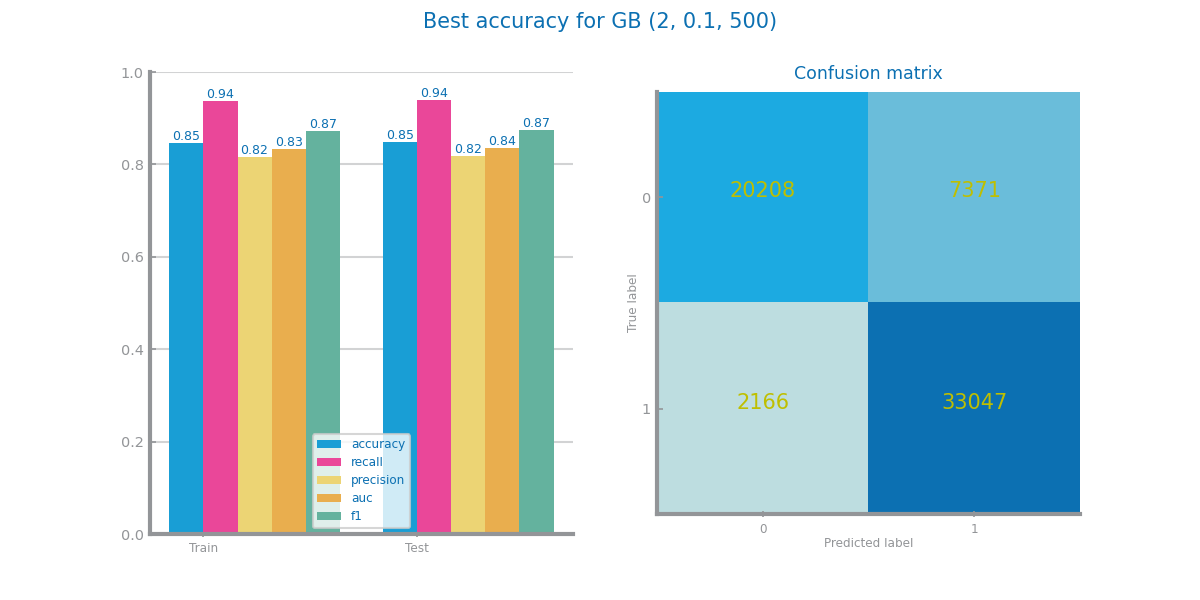
\includegraphics[width=\textwidth]{accidents_gb_GB_best_accuracy_eval.png}
    \end{subfigure}
    \hfill
    \begin{subfigure}[b]{0.45\textwidth}
        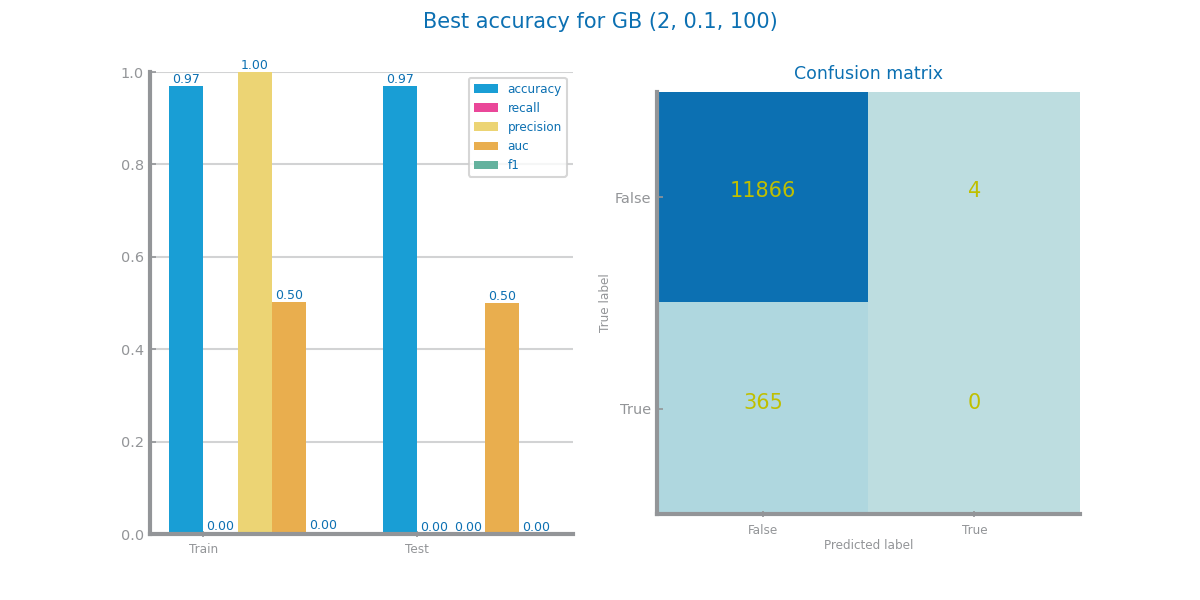
\includegraphics[width=\textwidth]{flights_gb_GB_best_accuracy_eval.png}
    \end{subfigure}
    \caption{Gradient boosting best model results for dataset 1 (left) and dataset 2 (right)}
\end{figure}

\begin{figure}[H]
    \centering
    \begin{subfigure}[b]{0.45\textwidth}
        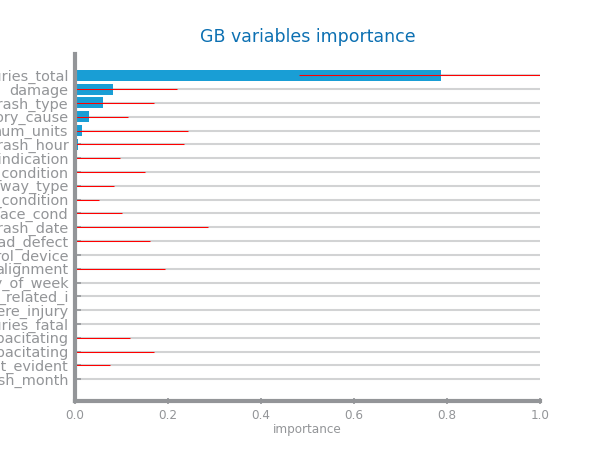
\includegraphics[width=\textwidth]{accidents_gb_accuracy_vars_ranking.png}
    \end{subfigure}
    \hfill
    \begin{subfigure}[b]{0.45\textwidth}
        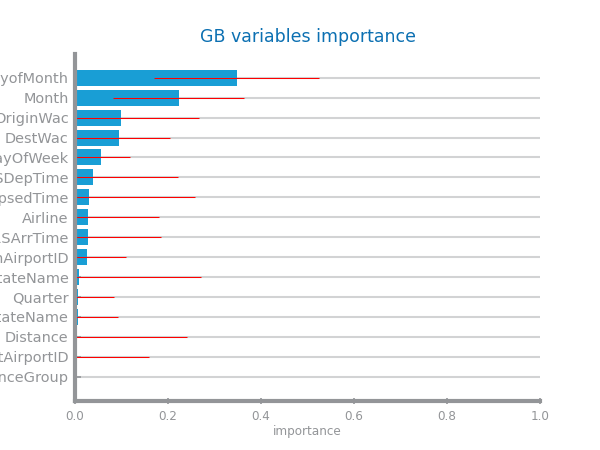
\includegraphics[width=\textwidth]{flights_gb_accuracy_vars_ranking.png}
    \end{subfigure}
    \caption{Gradient boosting variables importance for dataset 1 (left) and dataset 2 (right)}
\end{figure}

\subsection*{\textit{Multi-Layer Perceptrons}}
\ctext[RGB]{190,190,190}{Shall be used to present the results achieved through different parameterisations for the train of MLPs. The results shall be compared and explanations for them shall be presented. Shall be used to address the overfitting phenomenon, studying the conditions under which models face it. Shall be used to present the evaluation of the best model achieved.  \textbf{Shall not exceed 500 characters.}}

\begin{figure}[H]
\centering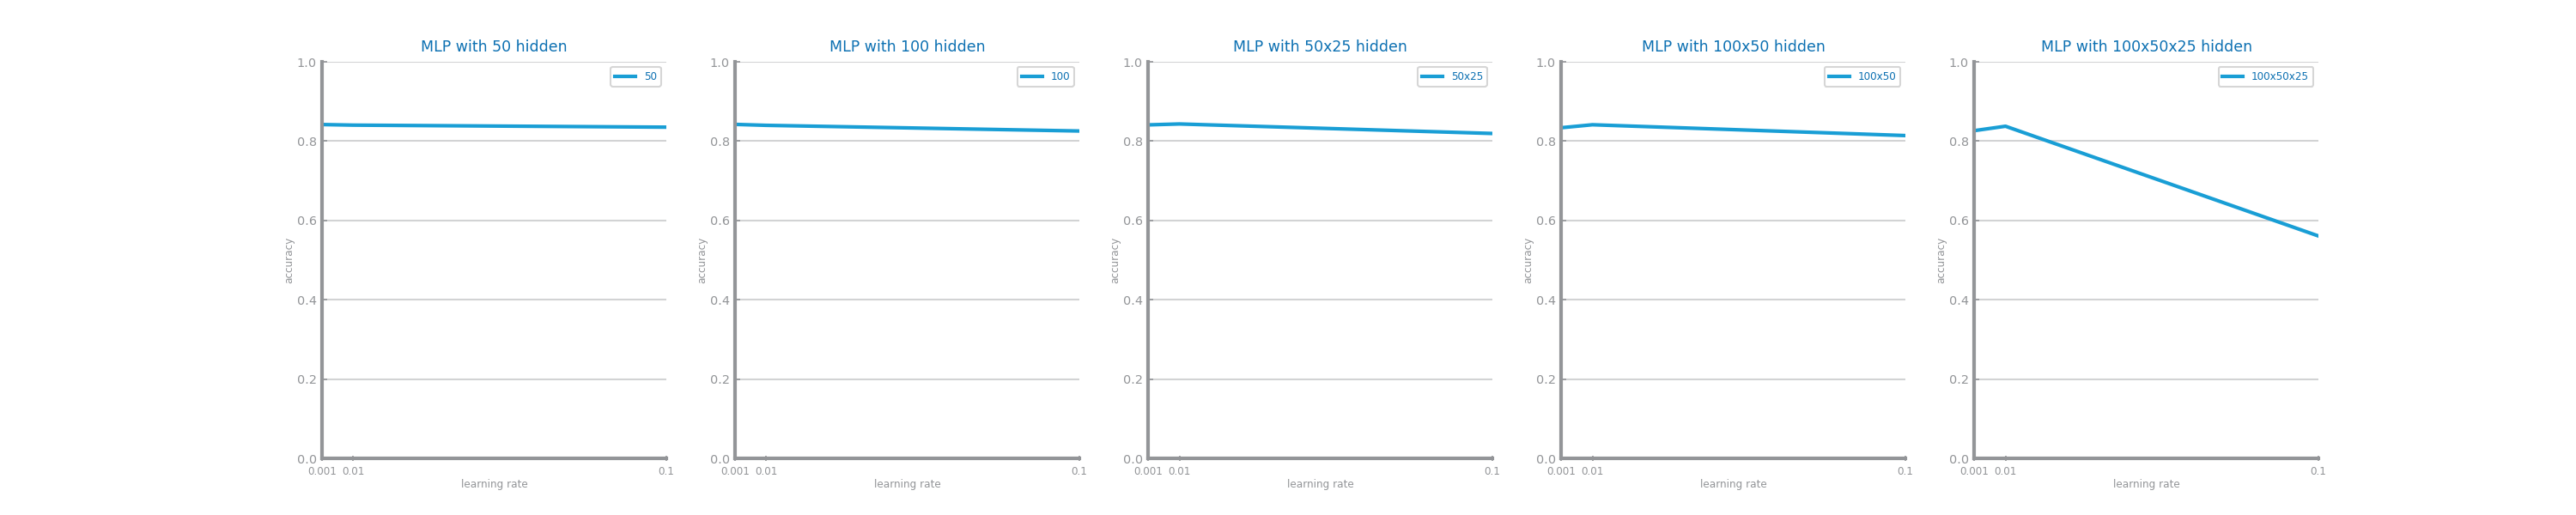
\includegraphics[width=0.9\textwidth]{accidents_mlp_accuracy_architecture_study.png}
\caption{MLP different parameterisations comparison for dataset 1}
\end{figure}

\begin{figure}[H]
\centering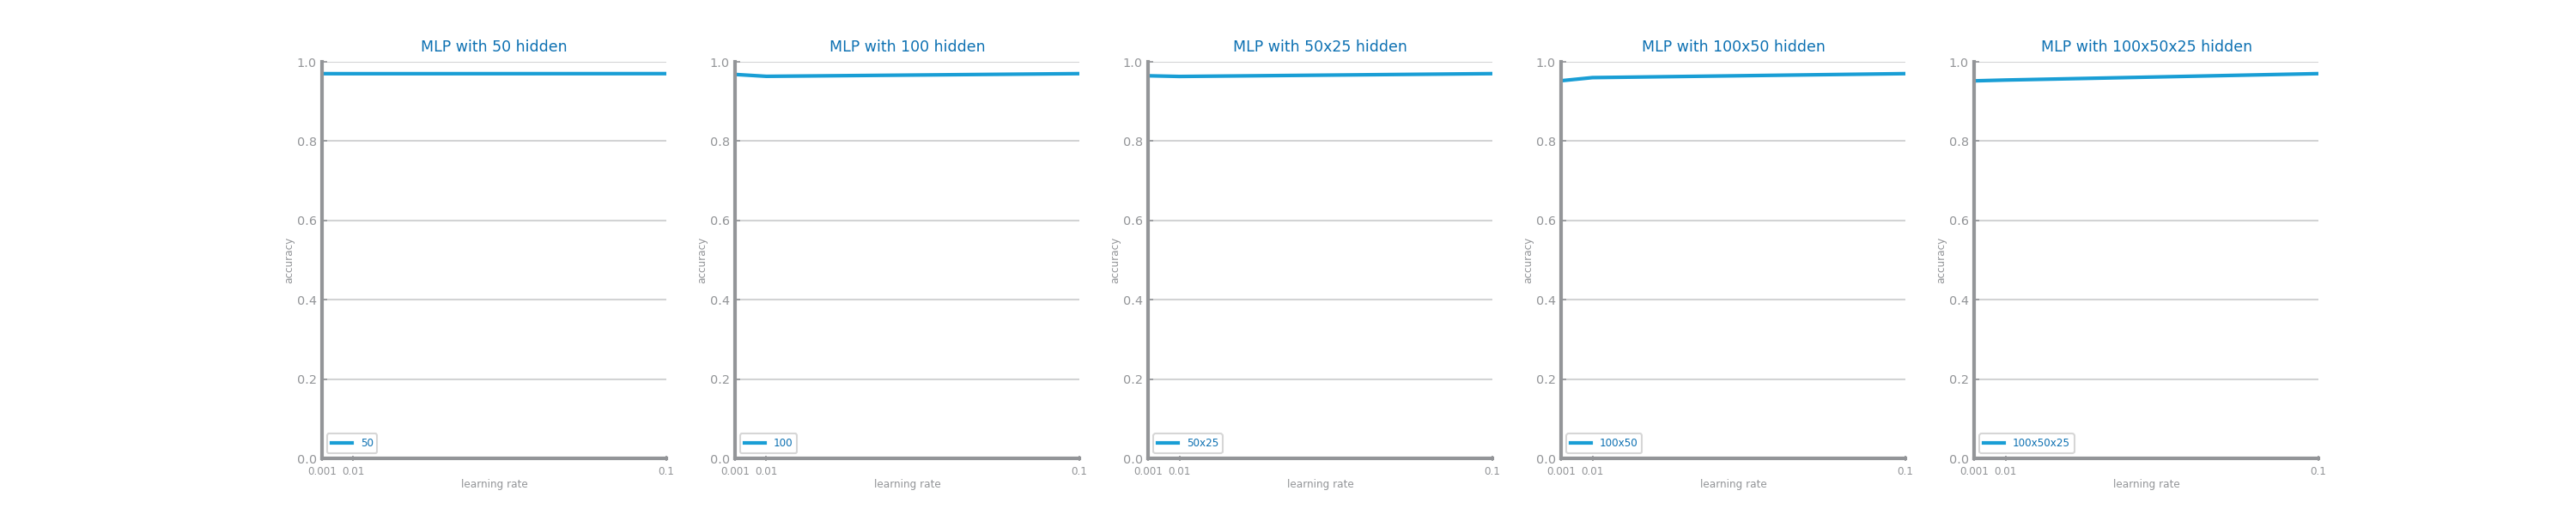
\includegraphics[width=0.9\textwidth]{flights_mlp_accuracy_architecture_study.png}
\caption{MLP different parameterisations comparison for dataset 2}
\end{figure}

\begin{figure}[H]
    \centering
    \begin{subfigure}[b]{0.45\textwidth}
        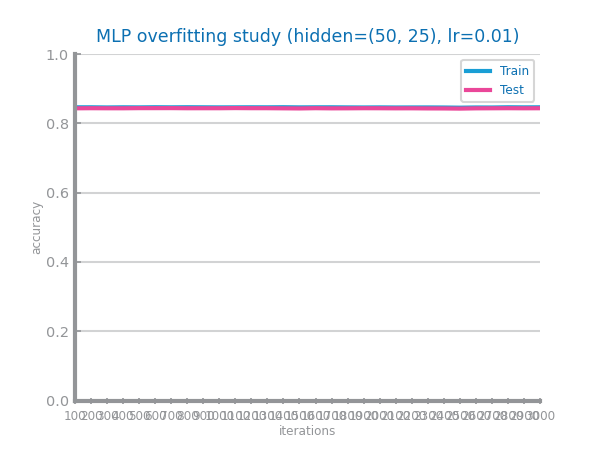
\includegraphics[width=\textwidth]{accidents_mlp_accuracy_overfitting.png}
    \end{subfigure}
    \hfill
    \begin{subfigure}[b]{0.45\textwidth}
        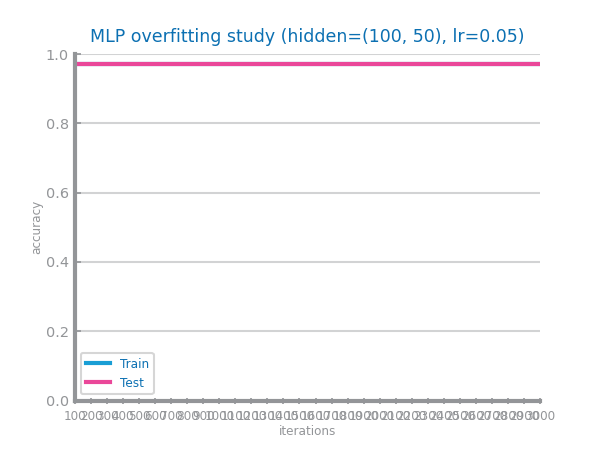
\includegraphics[width=\textwidth]{flights_mlp_accuracy_overfitting.png}
    \end{subfigure}
    \caption{MLP overfitting analysis for dataset 1 (left) and dataset 2 (right)}
\end{figure}

\begin{figure}[H]
    \centering
    \begin{subfigure}[b]{0.45\textwidth}
        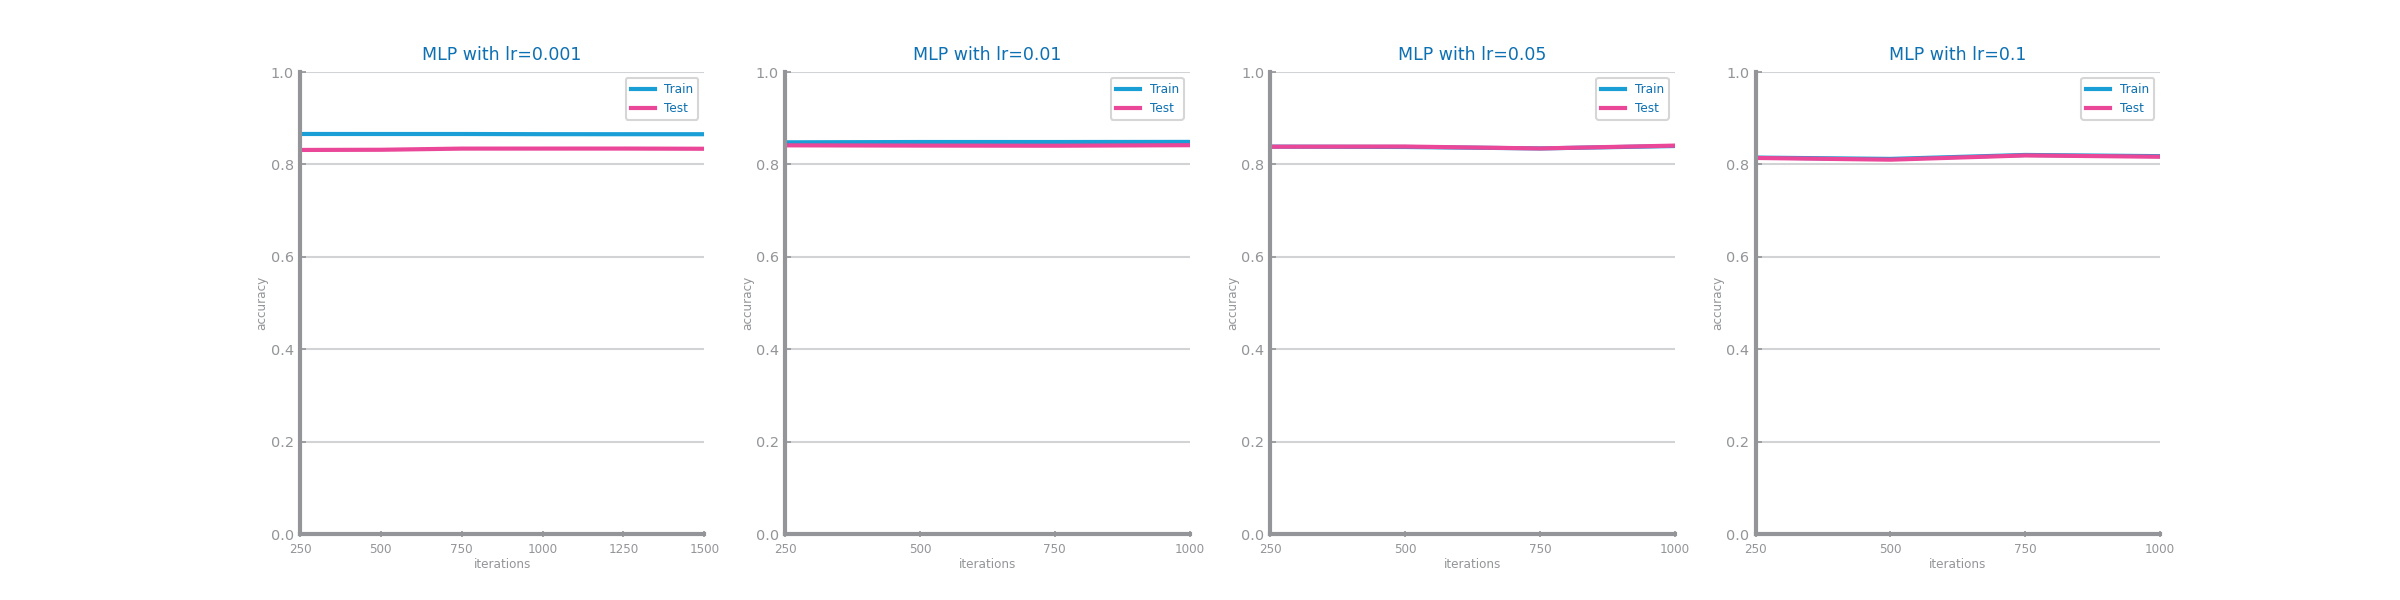
\includegraphics[width=\textwidth]{accidents_mlp_accuracy_iterations_study.png}
    \end{subfigure}
    \hfill
    \begin{subfigure}[b]{0.45\textwidth}
        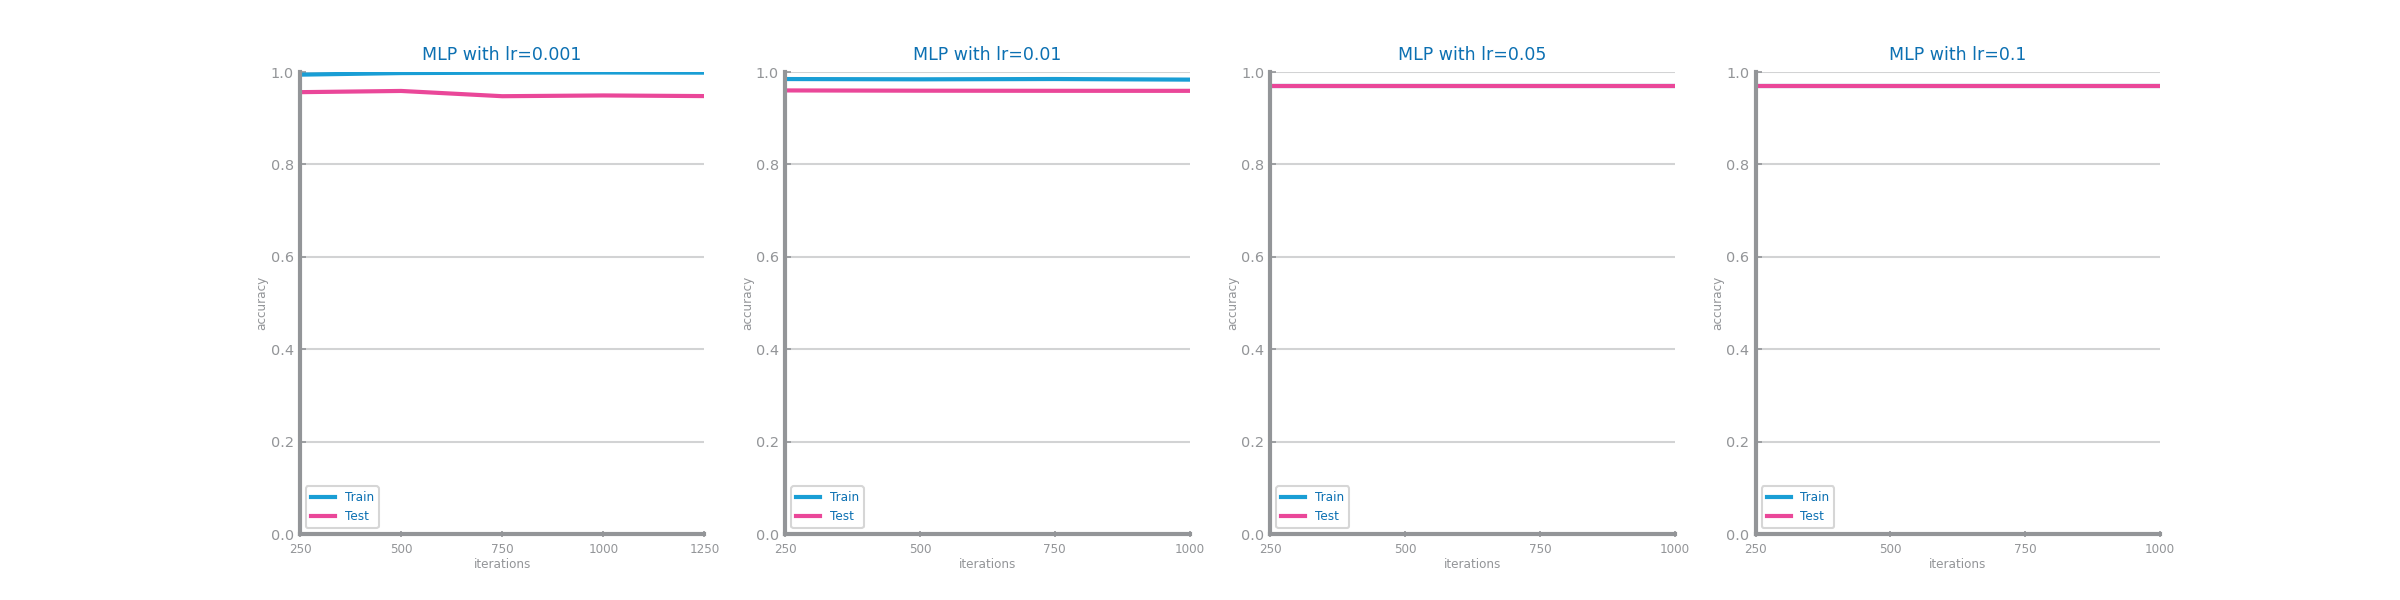
\includegraphics[width=\textwidth]{flights_mlp_accuracy_iterations_study.png}
    \end{subfigure}
    \caption{Loss curve analysis for dataset 1 (left) and dataset 2 (right)}
\end{figure}

\begin{figure}[H]
    \centering
    \begin{subfigure}[b]{0.45\textwidth}
        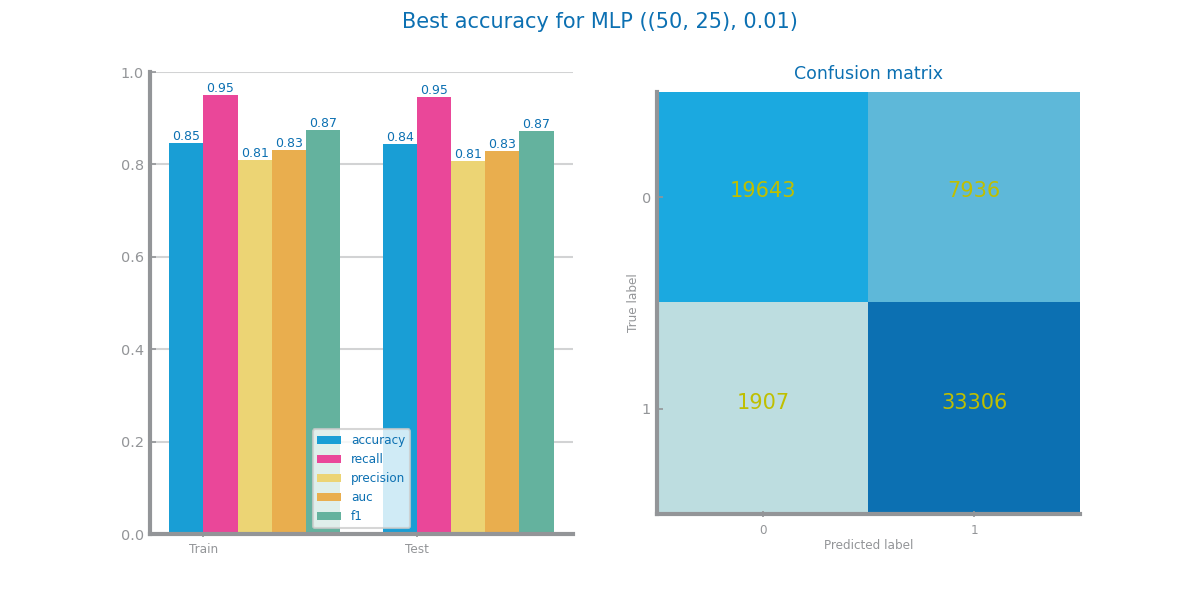
\includegraphics[width=\textwidth]{accidents_mlp_MLP_best_accuracy_eval.png}
    \end{subfigure}
    \hfill
    \begin{subfigure}[b]{0.45\textwidth}
        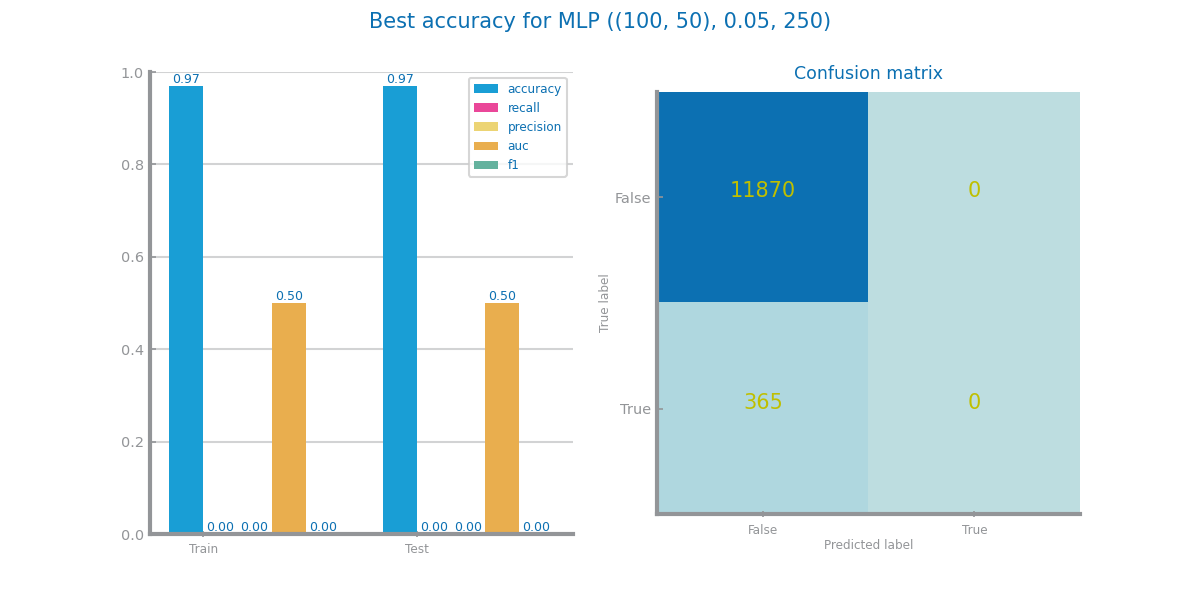
\includegraphics[width=\textwidth]{flights_mlp_MLP_best_accuracy_eval.png}
    \end{subfigure}
    \caption{MLP best model results for dataset 1 (left) and dataset 2 (right)}
\end{figure}

\section{CRITICAL ANALYSIS}
\ctext[RGB]{190,190,190}{Shall be used to present a summary of the results achieved with the different modelling techniques, and the impact of the different preparation tasks on their performance. 
A cross-analysis of the different models may also be presented, identifying the most relevant variables common to all of them (when possible) and the relation among the patterns identified within the different classifiers.
A critical assessment of the best models shall be presented, clearly stating if the models seem to be good enough for the problem at hand. \textbf{Additional charts may be presented here.  Shall not exceed 2000 characters.}}


\begin{center}
	\section*{\fontsize{0.75cm}{1cm}\selectfont TIME SERIES ANALYSIS}
\end{center}

\section{DATA PROFILING}

\subsection*{\textit{Data Dimensionality and Granularity}}
\ctext[RGB]{190,190,190}{May be used to identify the most atomic granularity and two other different granularities to consider.  \textbf{Shall not exceed 500 characters.}}

\begin{figure}[H]
\centering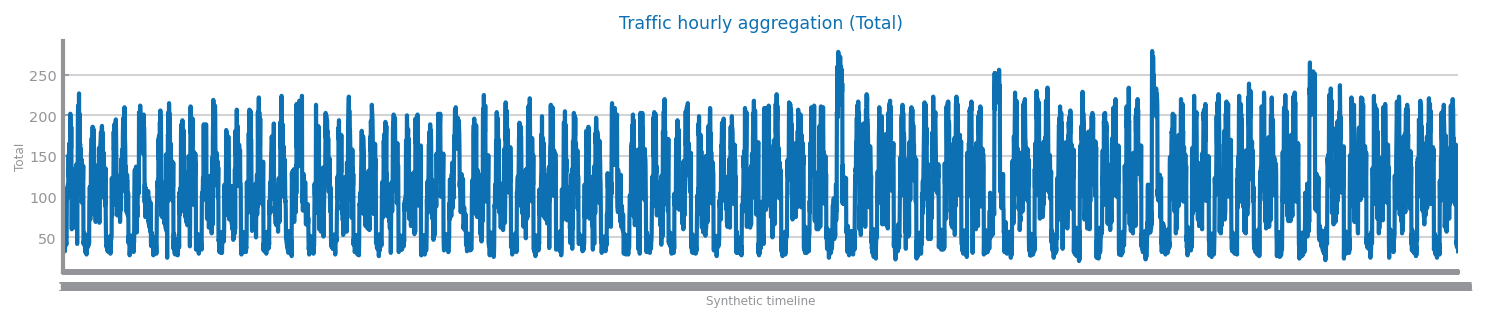
\includegraphics[width=0.9\textwidth]{traffic_hourly.png}
\caption{Time series 1 at the most granular detail}
\end{figure}

\begin{figure}[H]
\centering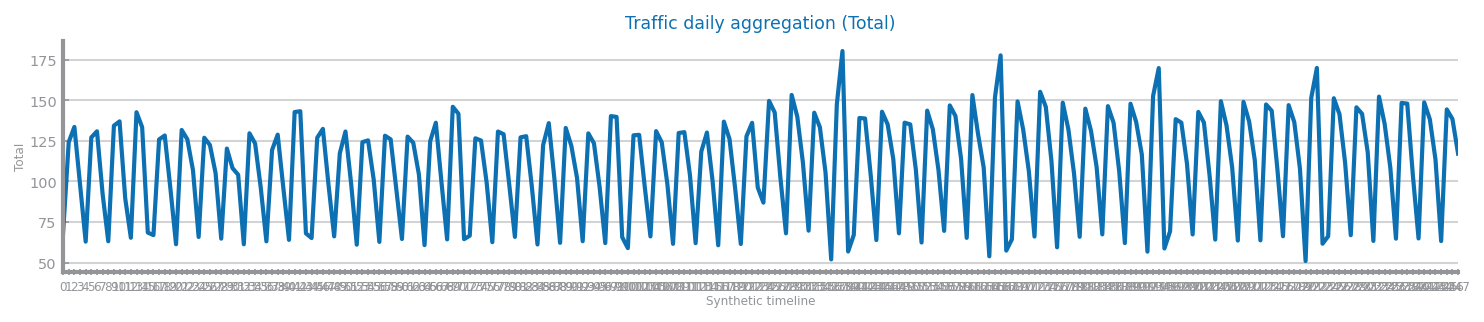
\includegraphics[width=0.9\textwidth]{traffic_daily.png}
\caption{Time series 1 at the second chosen granularity}
\end{figure}

\begin{figure}[H]
\centering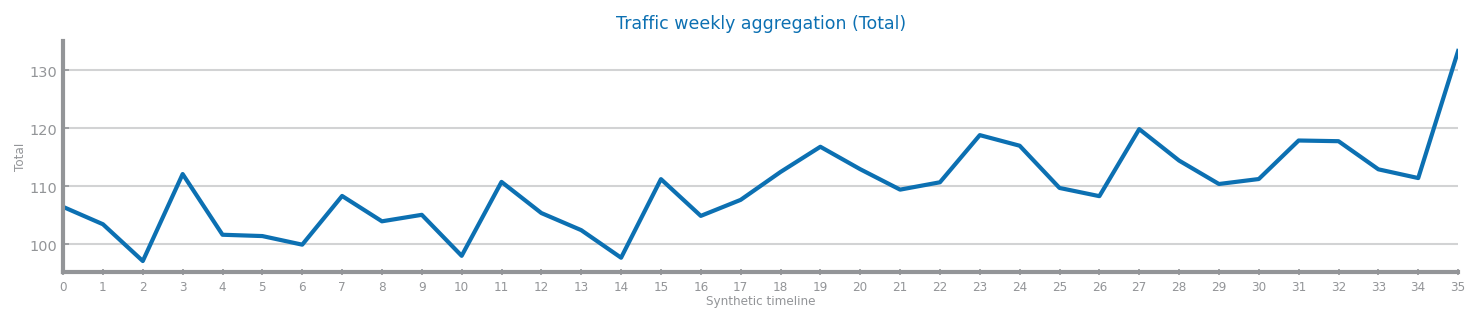
\includegraphics[width=0.9\textwidth]{traffic_weekly.png}
\caption{Time series 1 at the third chosen granularity}
\end{figure}

\begin{figure}[H]
\centering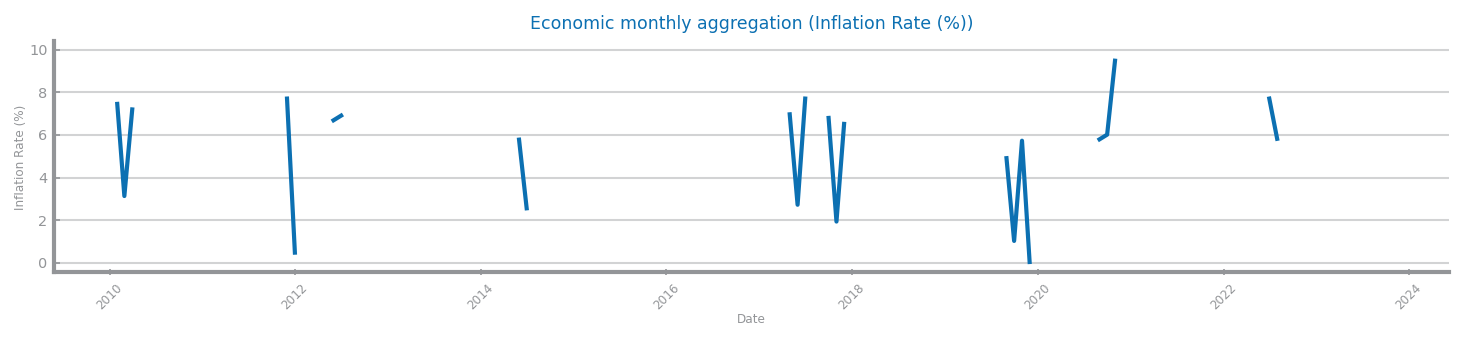
\includegraphics[width=0.9\textwidth]{economic_monthly.png}
\caption{Time series 2 at the most granular detail}
\end{figure}

\begin{figure}[H]
\centering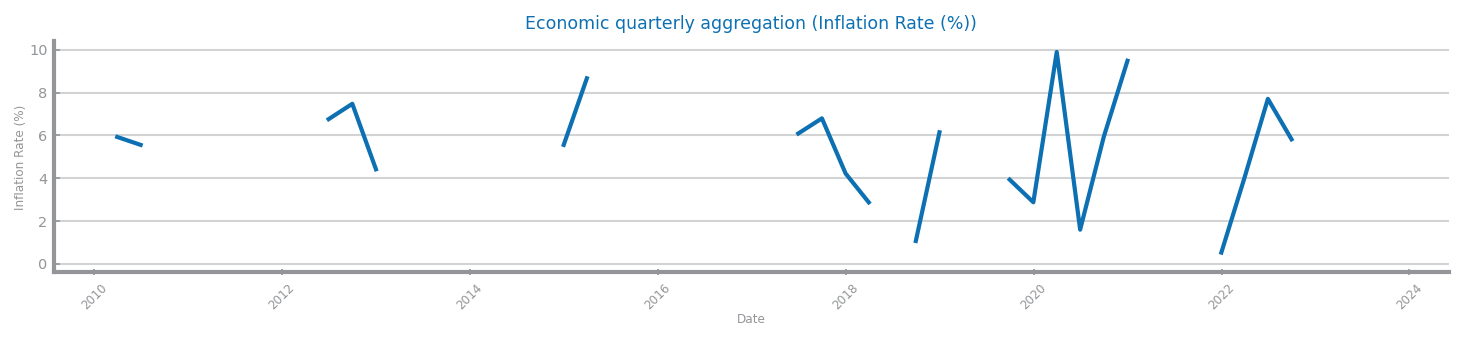
\includegraphics[width=0.9\textwidth]{economic_quarterly.png}
\caption{Time series 2 at the second chosen granularity}
\end{figure}

\begin{figure}[H]
\centering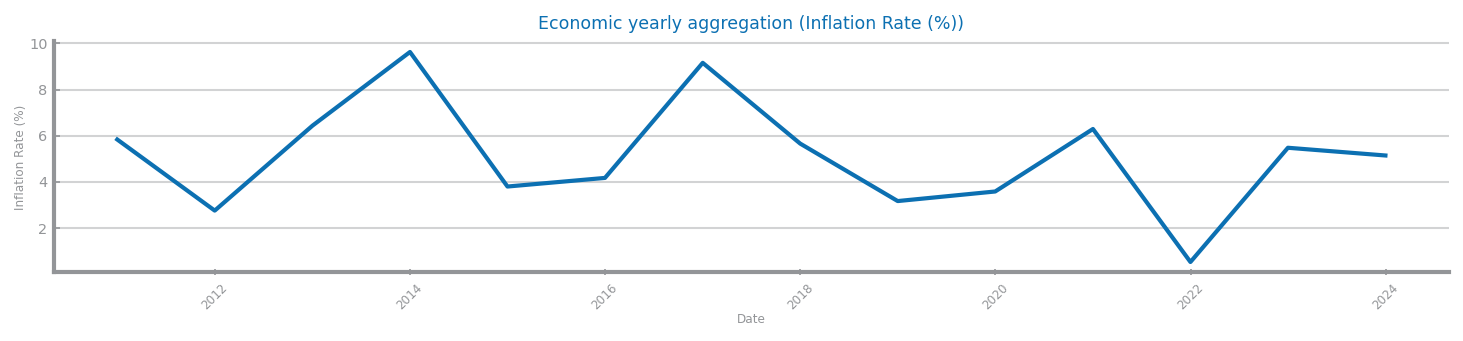
\includegraphics[width=0.9\textwidth]{economic_yearly.png}
\caption{Time series 2 at the third chosen granularity}
\end{figure}

\subsection*{\textit{Data Distribution}}
\ctext[RGB]{190,190,190}{Shall be used to perform the data analysis at those three different granularities, concerning the series distribution.  \textbf{Shall not exceed 500 characters.}}

\begin{figure}[H]
\centering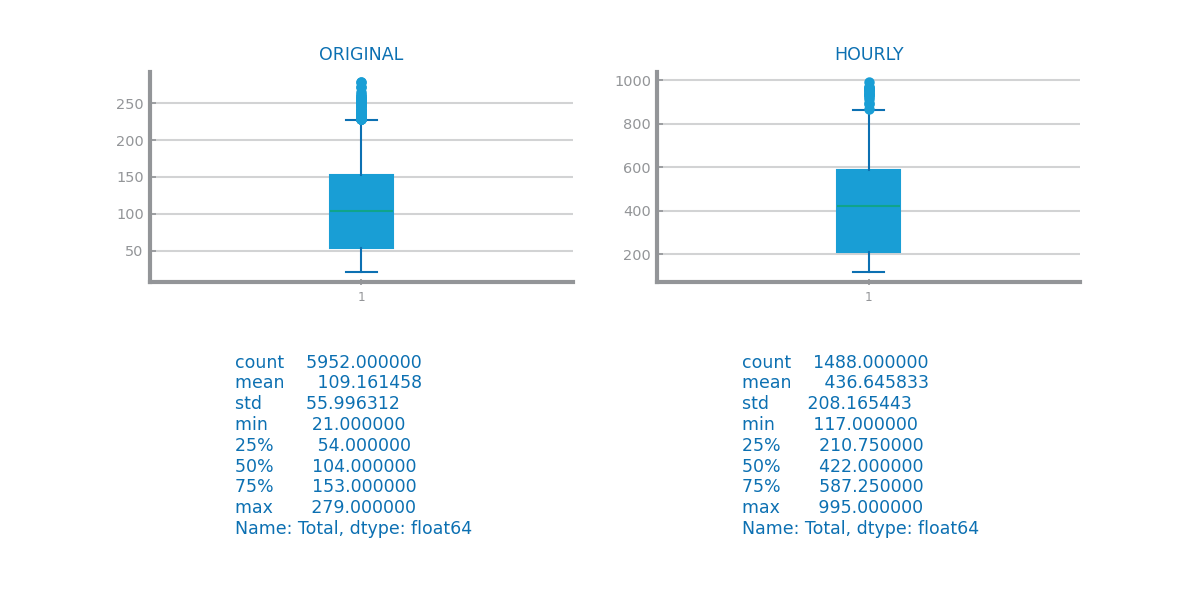
\includegraphics[width=0.9\textwidth]{Traffic_distribution_boxplots.png}
\caption{Boxplot(s) for time series 1}
\end{figure}

\begin{figure}[H]
\centering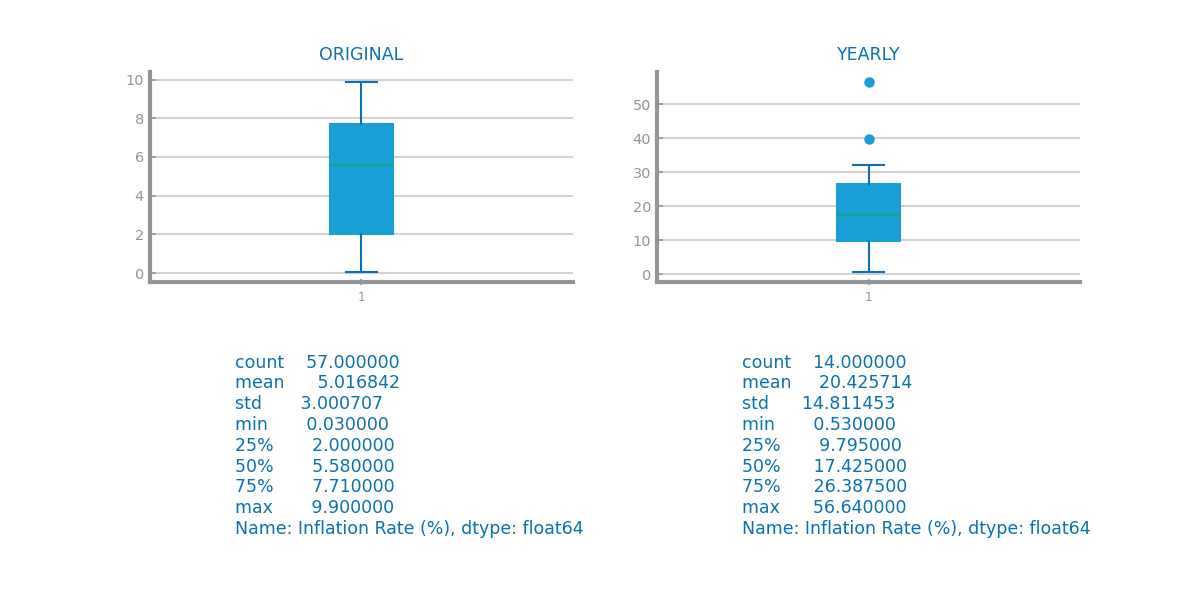
\includegraphics[width=0.9\textwidth]{Economic_distribution_boxplots.png}
\caption{Boxplot(s) for time series 2}
\end{figure}

\begin{figure}[H]
\centering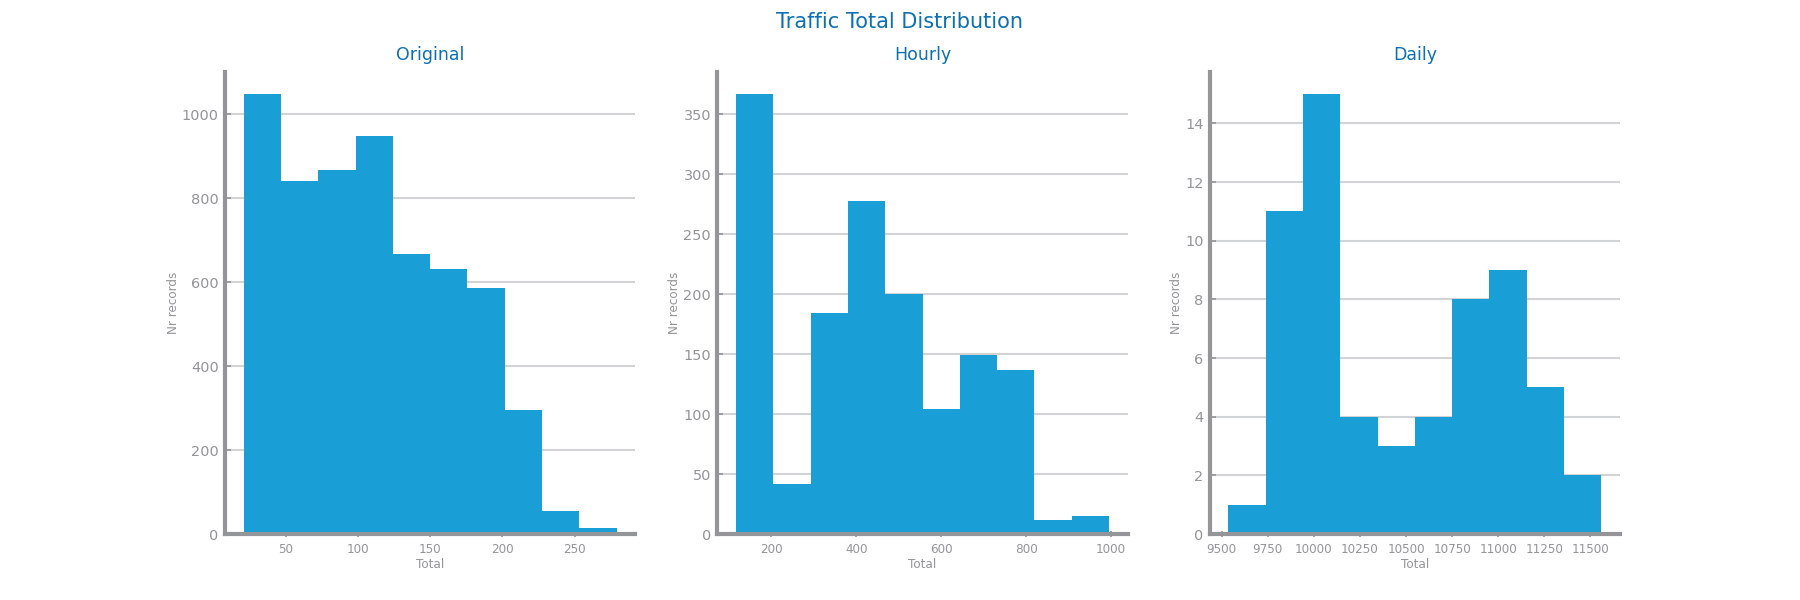
\includegraphics[width=0.9\textwidth]{Traffic_distribution_histograms.png}
\caption{Histogram(s) for time series 1}
\end{figure}

\begin{figure}[H]
\centering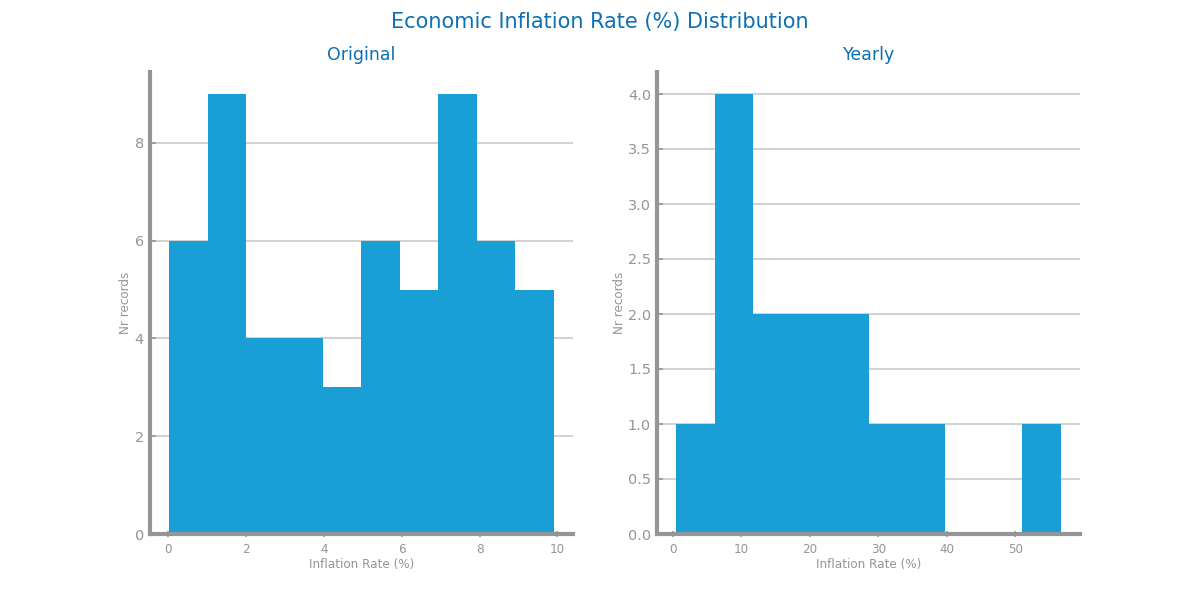
\includegraphics[width=0.9\textwidth]{Economic_distribution_histograms.png}
\caption{Histogram(s) for time series 2}
\end{figure}

\begin{figure}[H]
\centering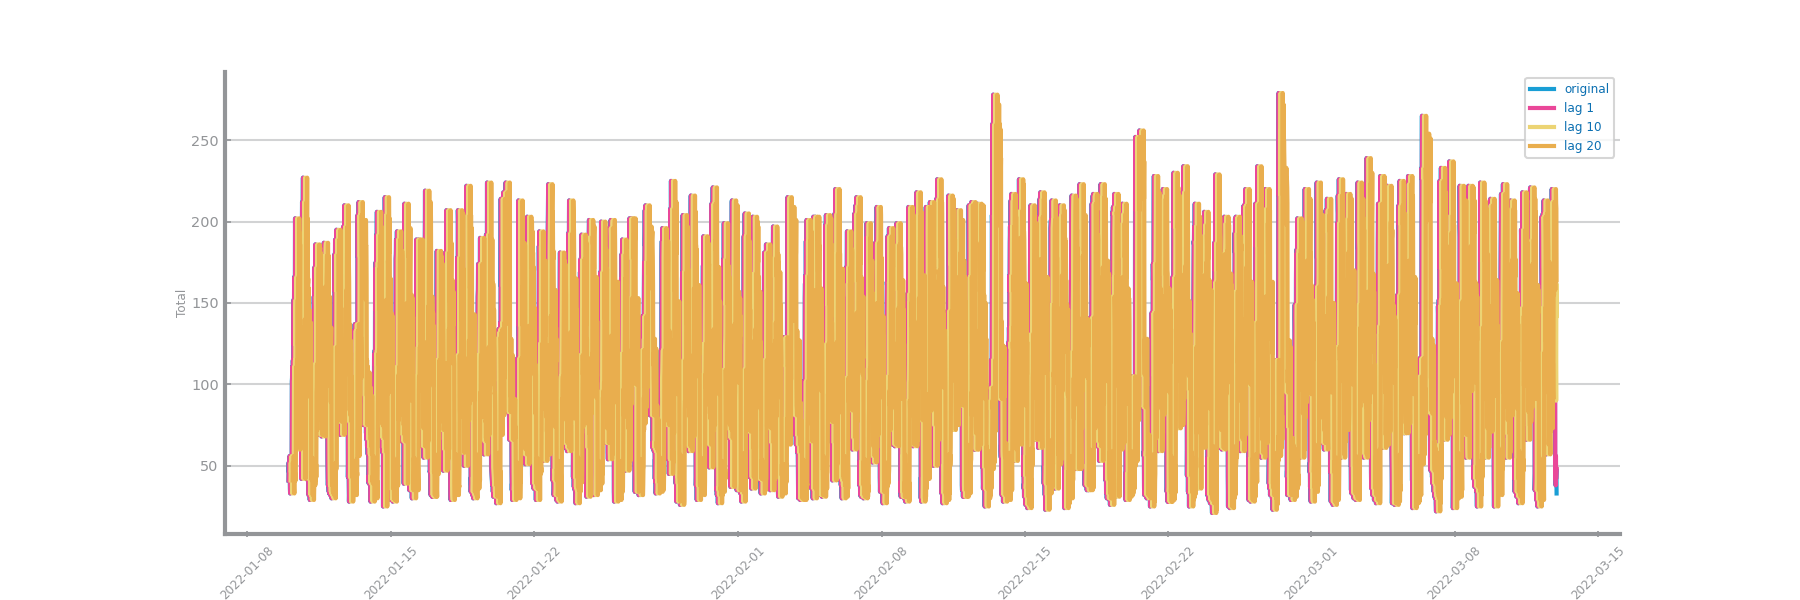
\includegraphics[width=0.9\textwidth]{Traffic_lag_plot.png}
\caption{Autocorrelation lag-plots for original time series 1}
\end{figure}

\begin{figure}[H]
\centering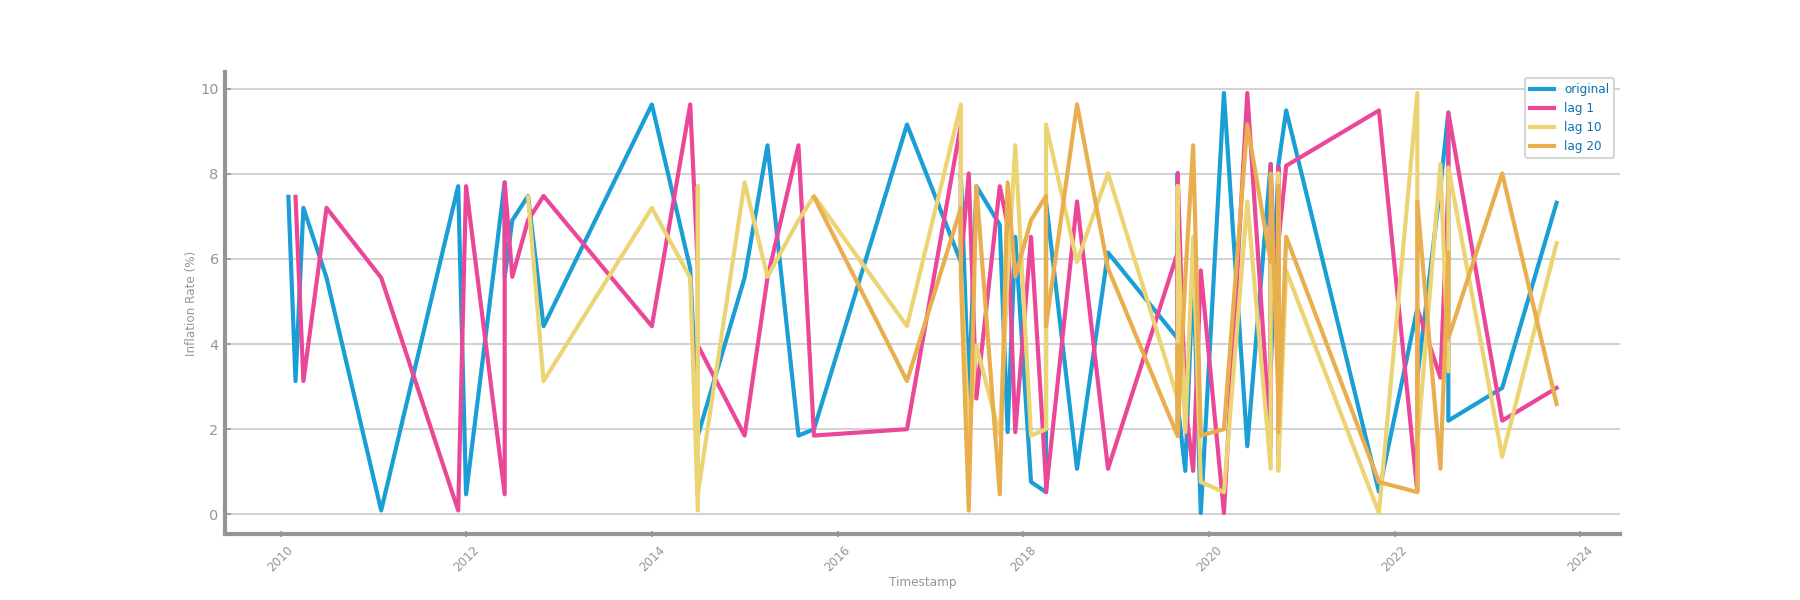
\includegraphics[width=0.9\textwidth]{Economic_lag_plot.png}
\caption{Autocorrelation lag-plots for original time series 2}
\end{figure}

\begin{figure}[H]
\centering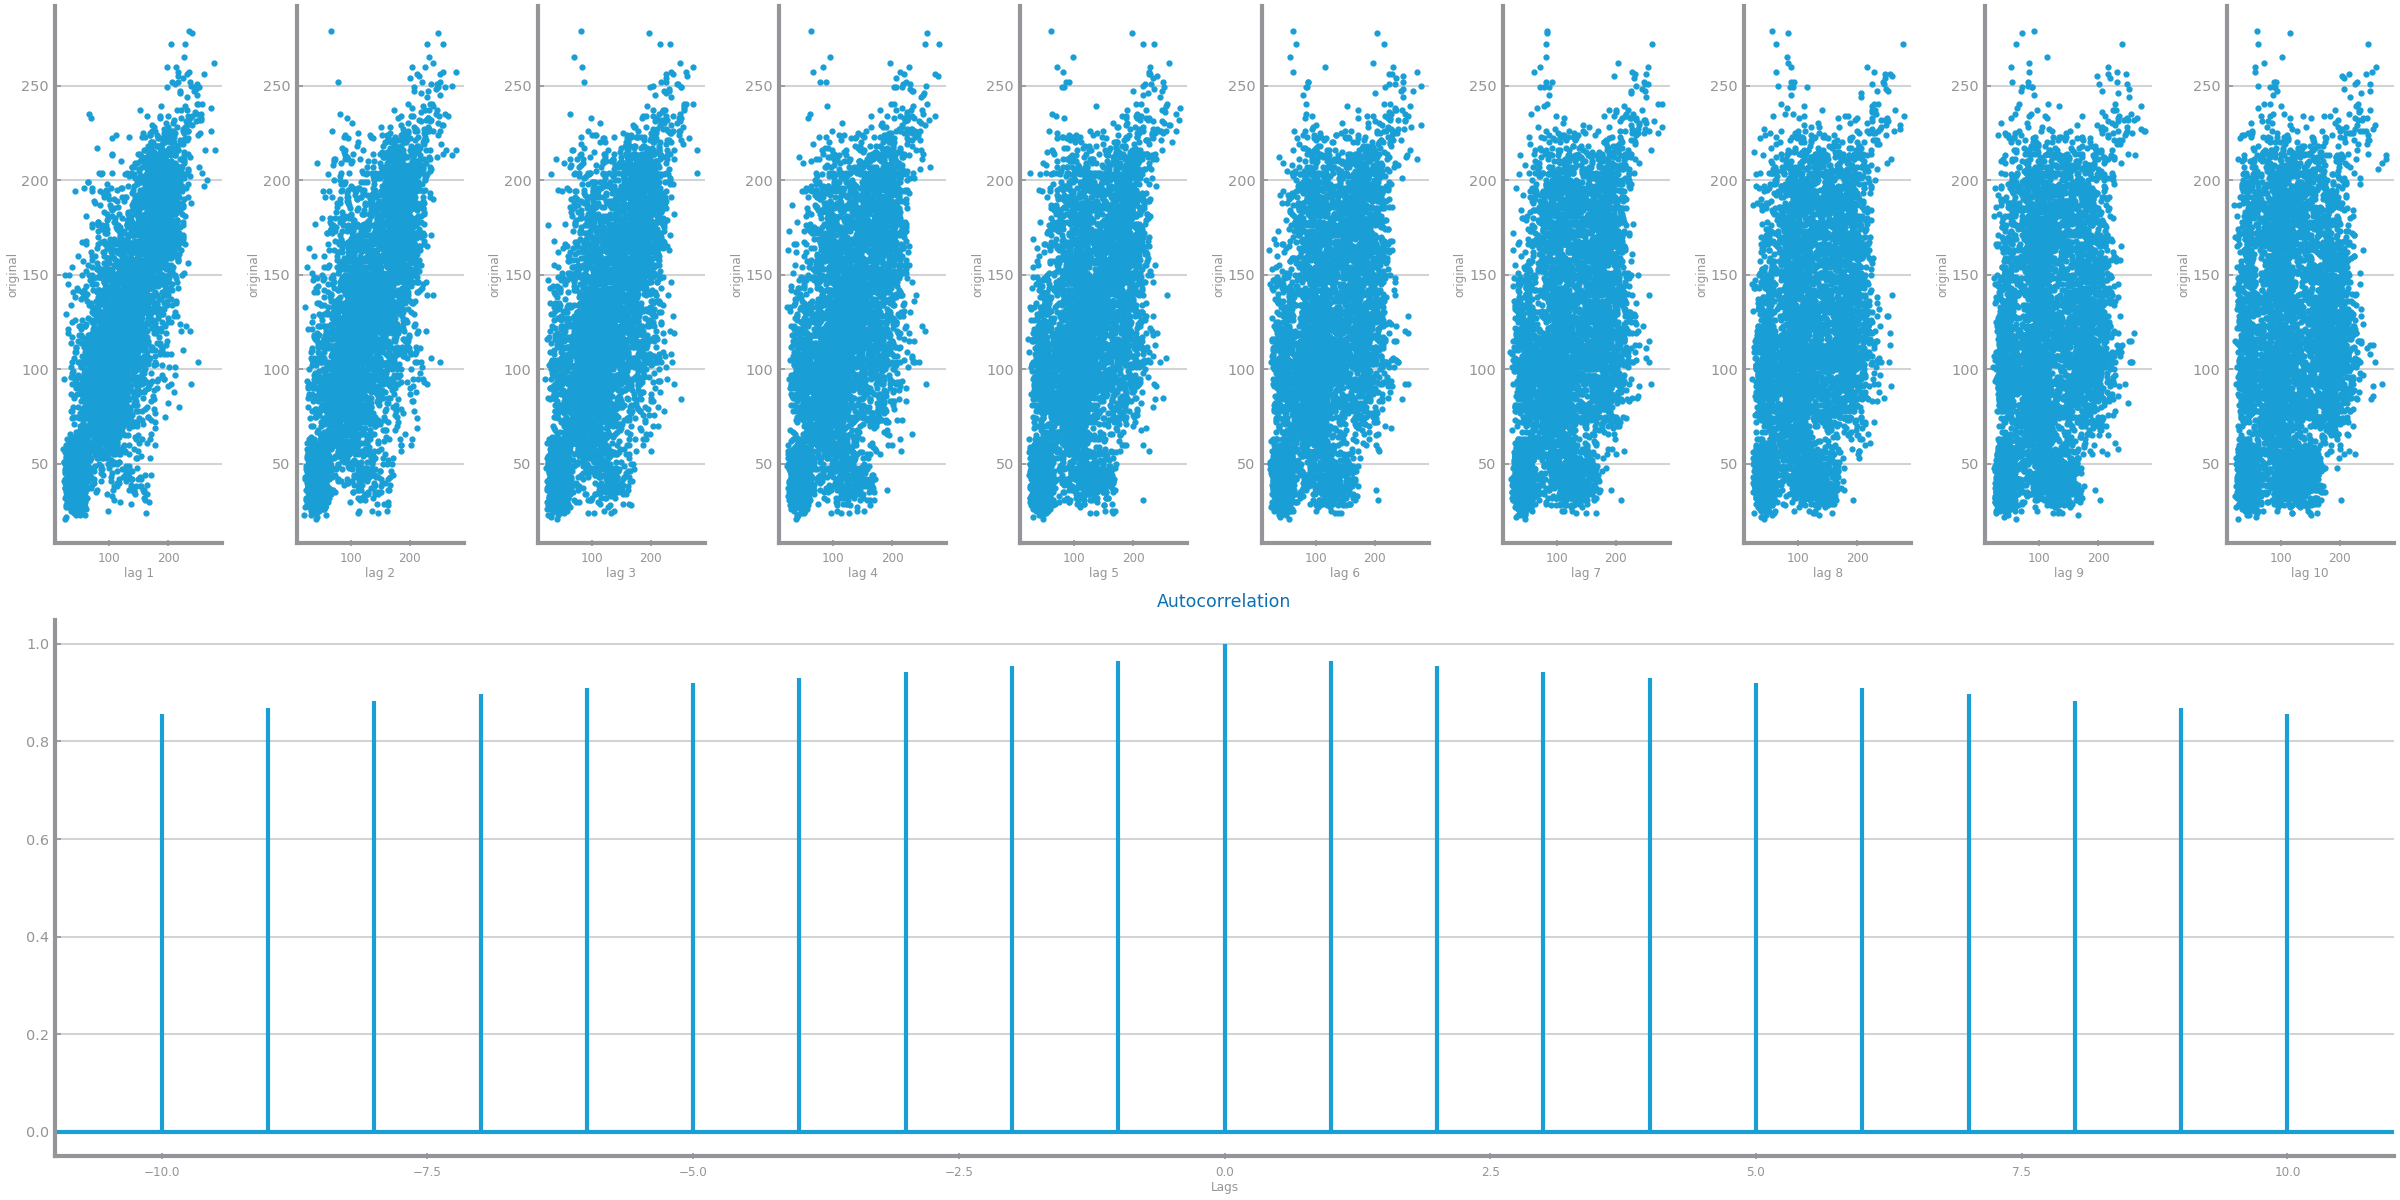
\includegraphics[width=0.9\textwidth]{Traffic_autocorrelation.png}
\caption{Autocorrelation correlogram for original time series 1}
\end{figure}

\begin{figure}[H]
\centering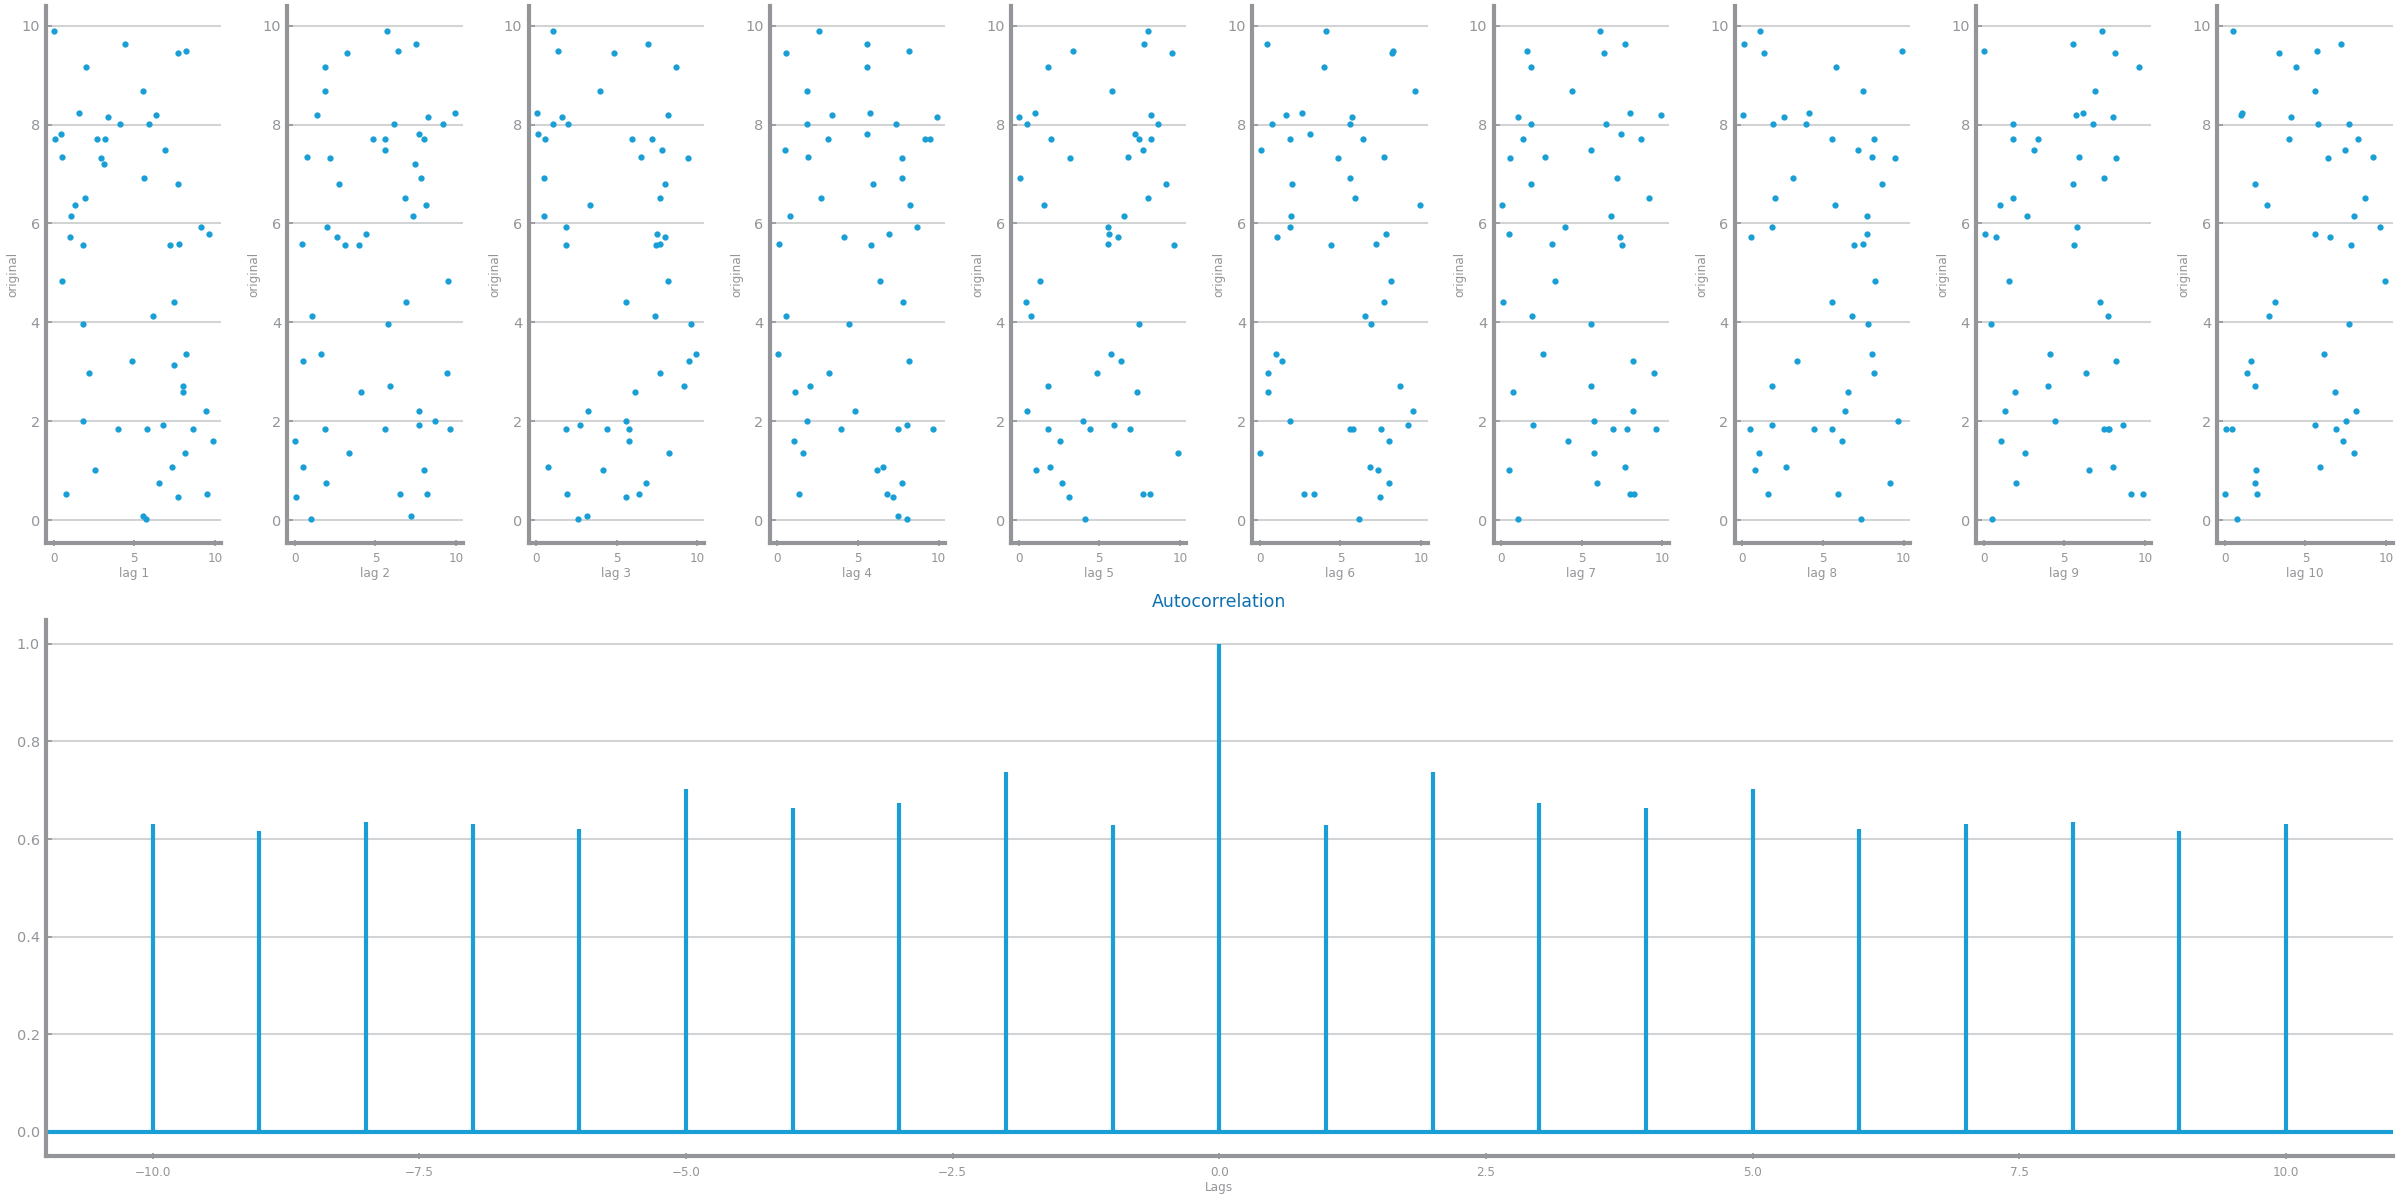
\includegraphics[width=0.9\textwidth]{Economic_autocorrelation.png}
\caption{Autocorrelation correlogram for original time series 2}
\end{figure}

\subsection*{\textit{Data Stationarity}}
\ctext[RGB]{190,190,190}{Shall be used to perform the data analysis at those three different granularities, concerning the series stationarity.  \textbf{Shall not exceed 300 characters.}}

\begin{figure}[H]
\centering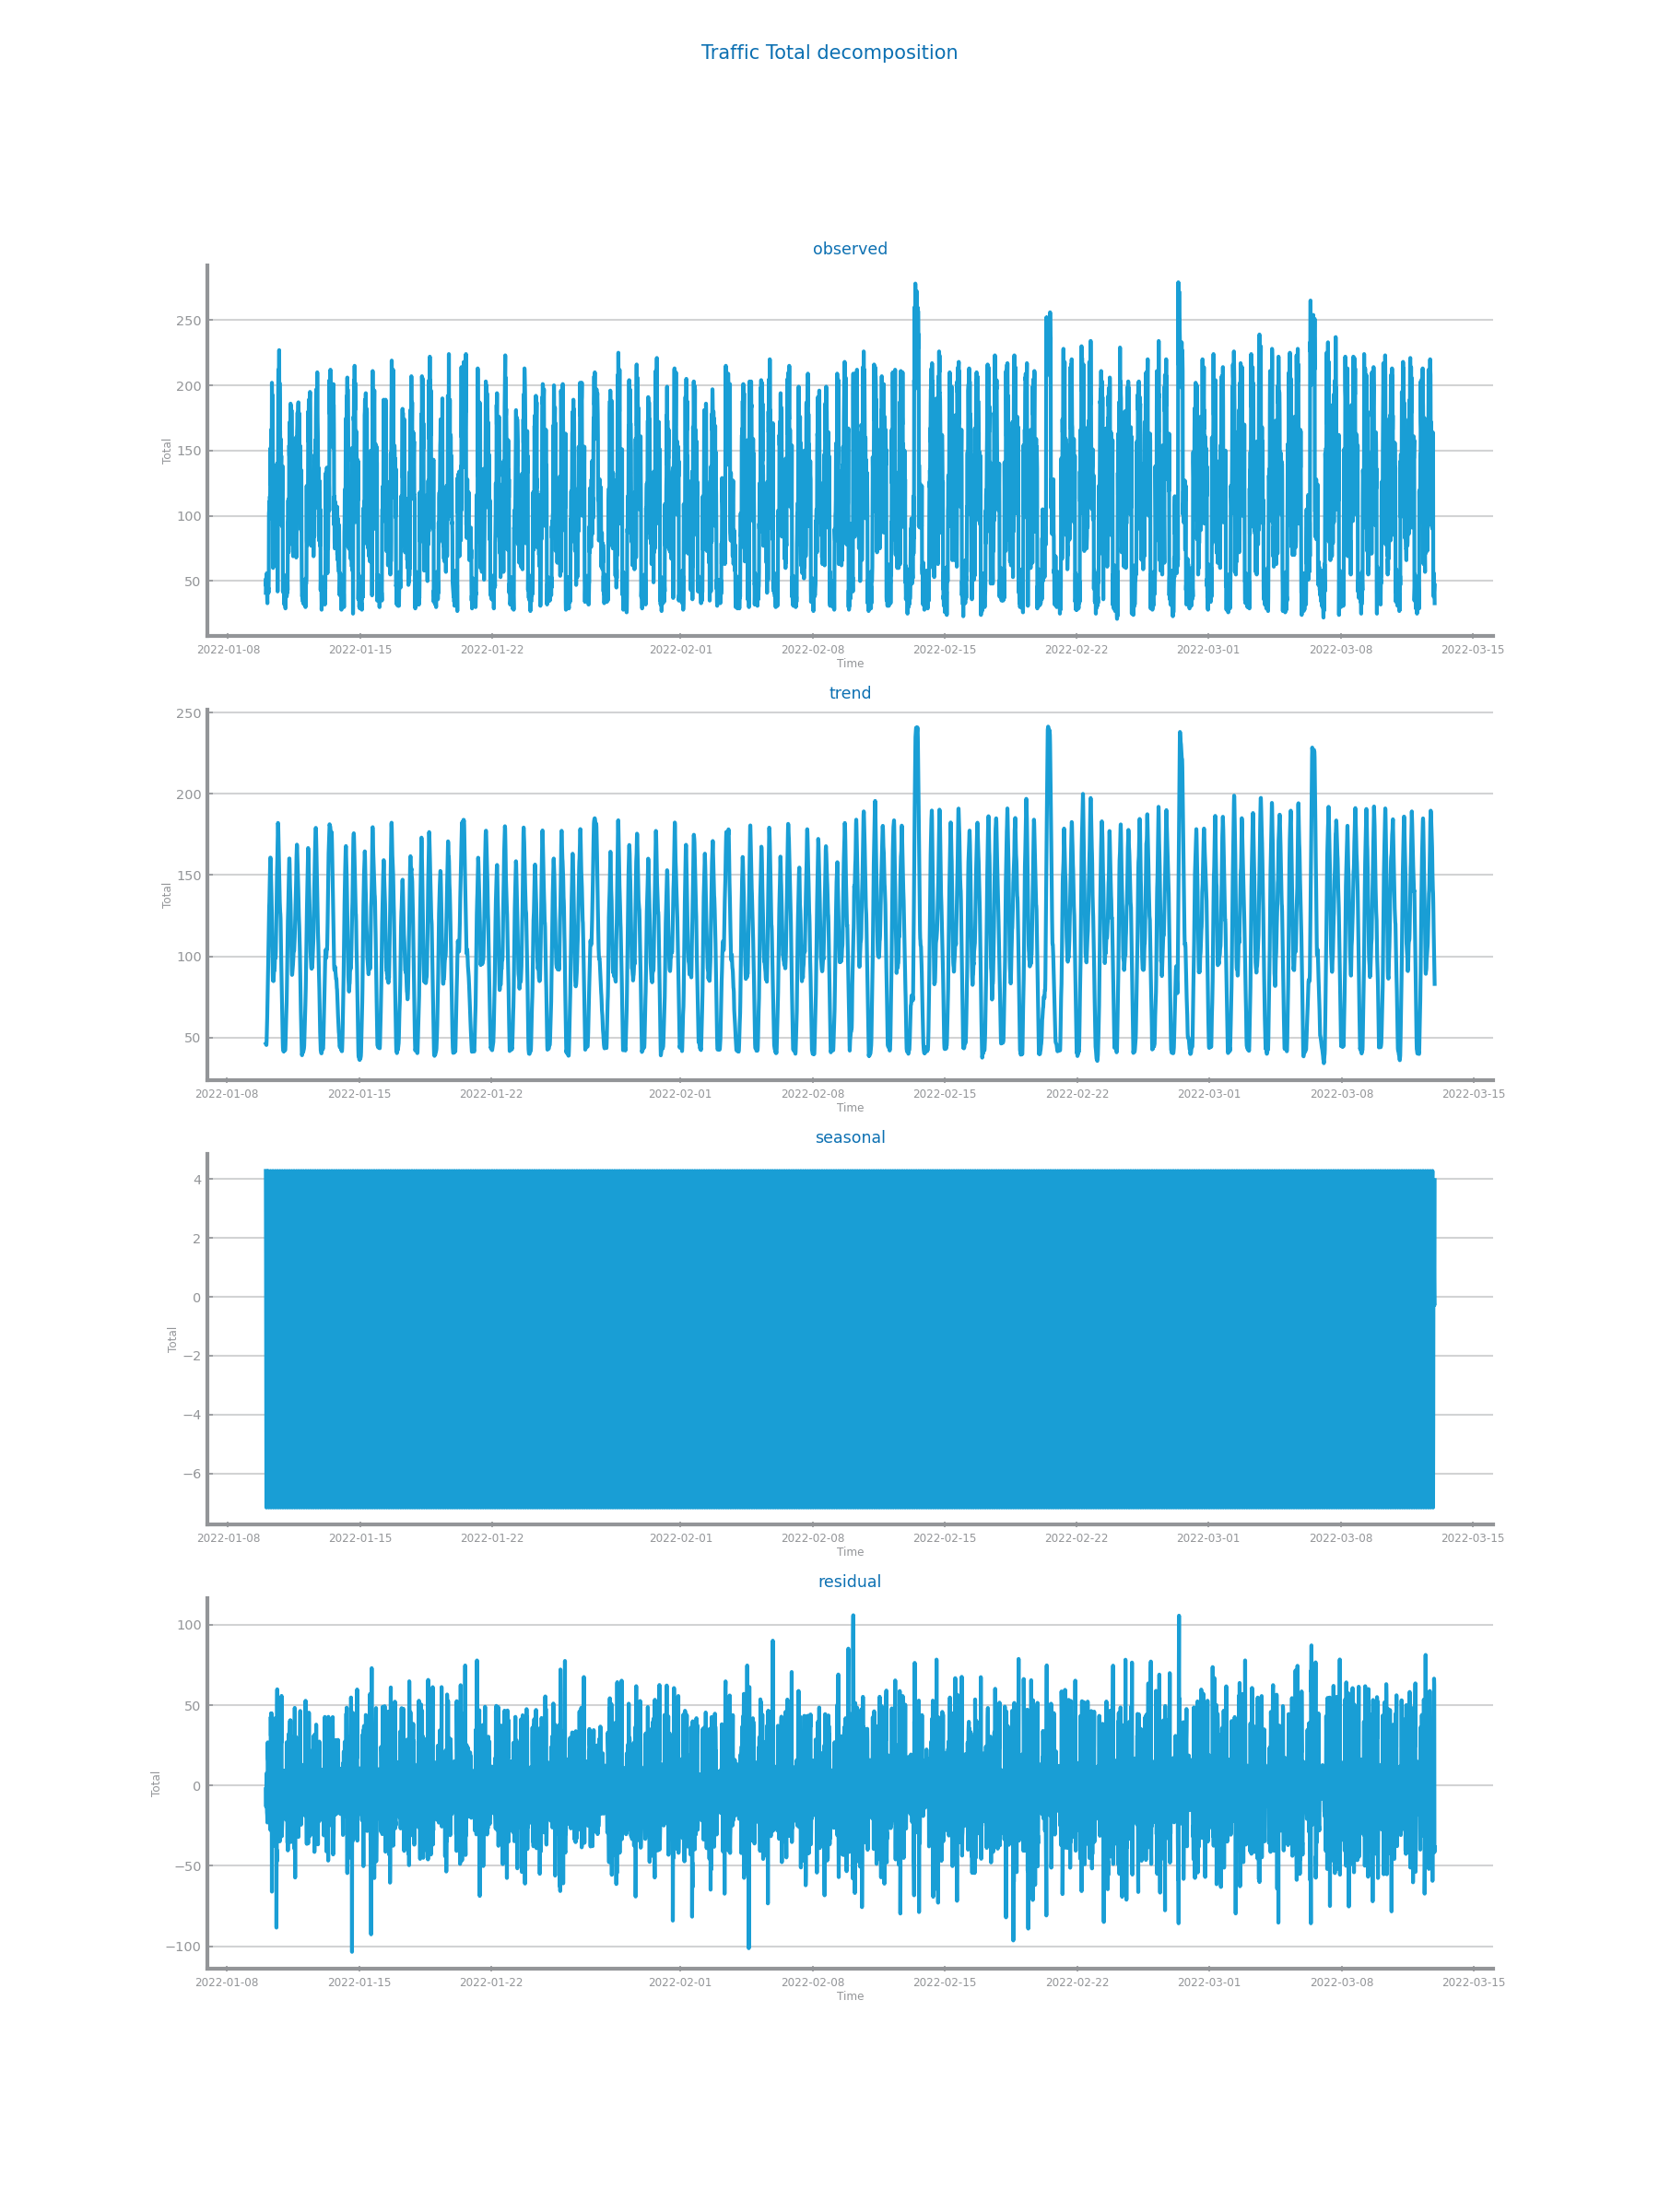
\includegraphics[width=0.9\textwidth]{Traffic_seasonality.png}
\caption{Components study for time series 1}
\end{figure}


\begin{figure}[H]
\centering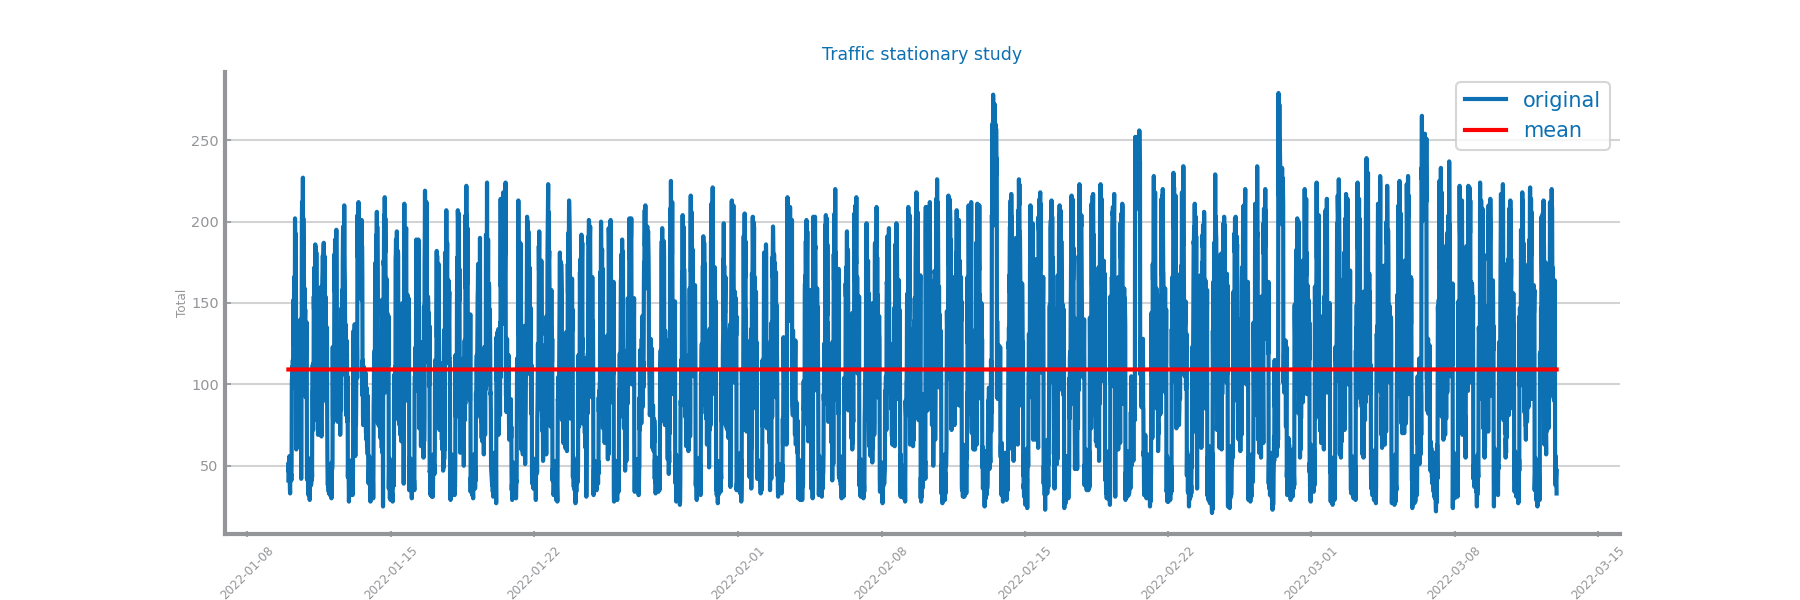
\includegraphics[width=0.9\textwidth]{Traffic_stationarity_mean.png}
\caption{Stationarity study for time series 1}
\end{figure}

\begin{figure}[H]
\centering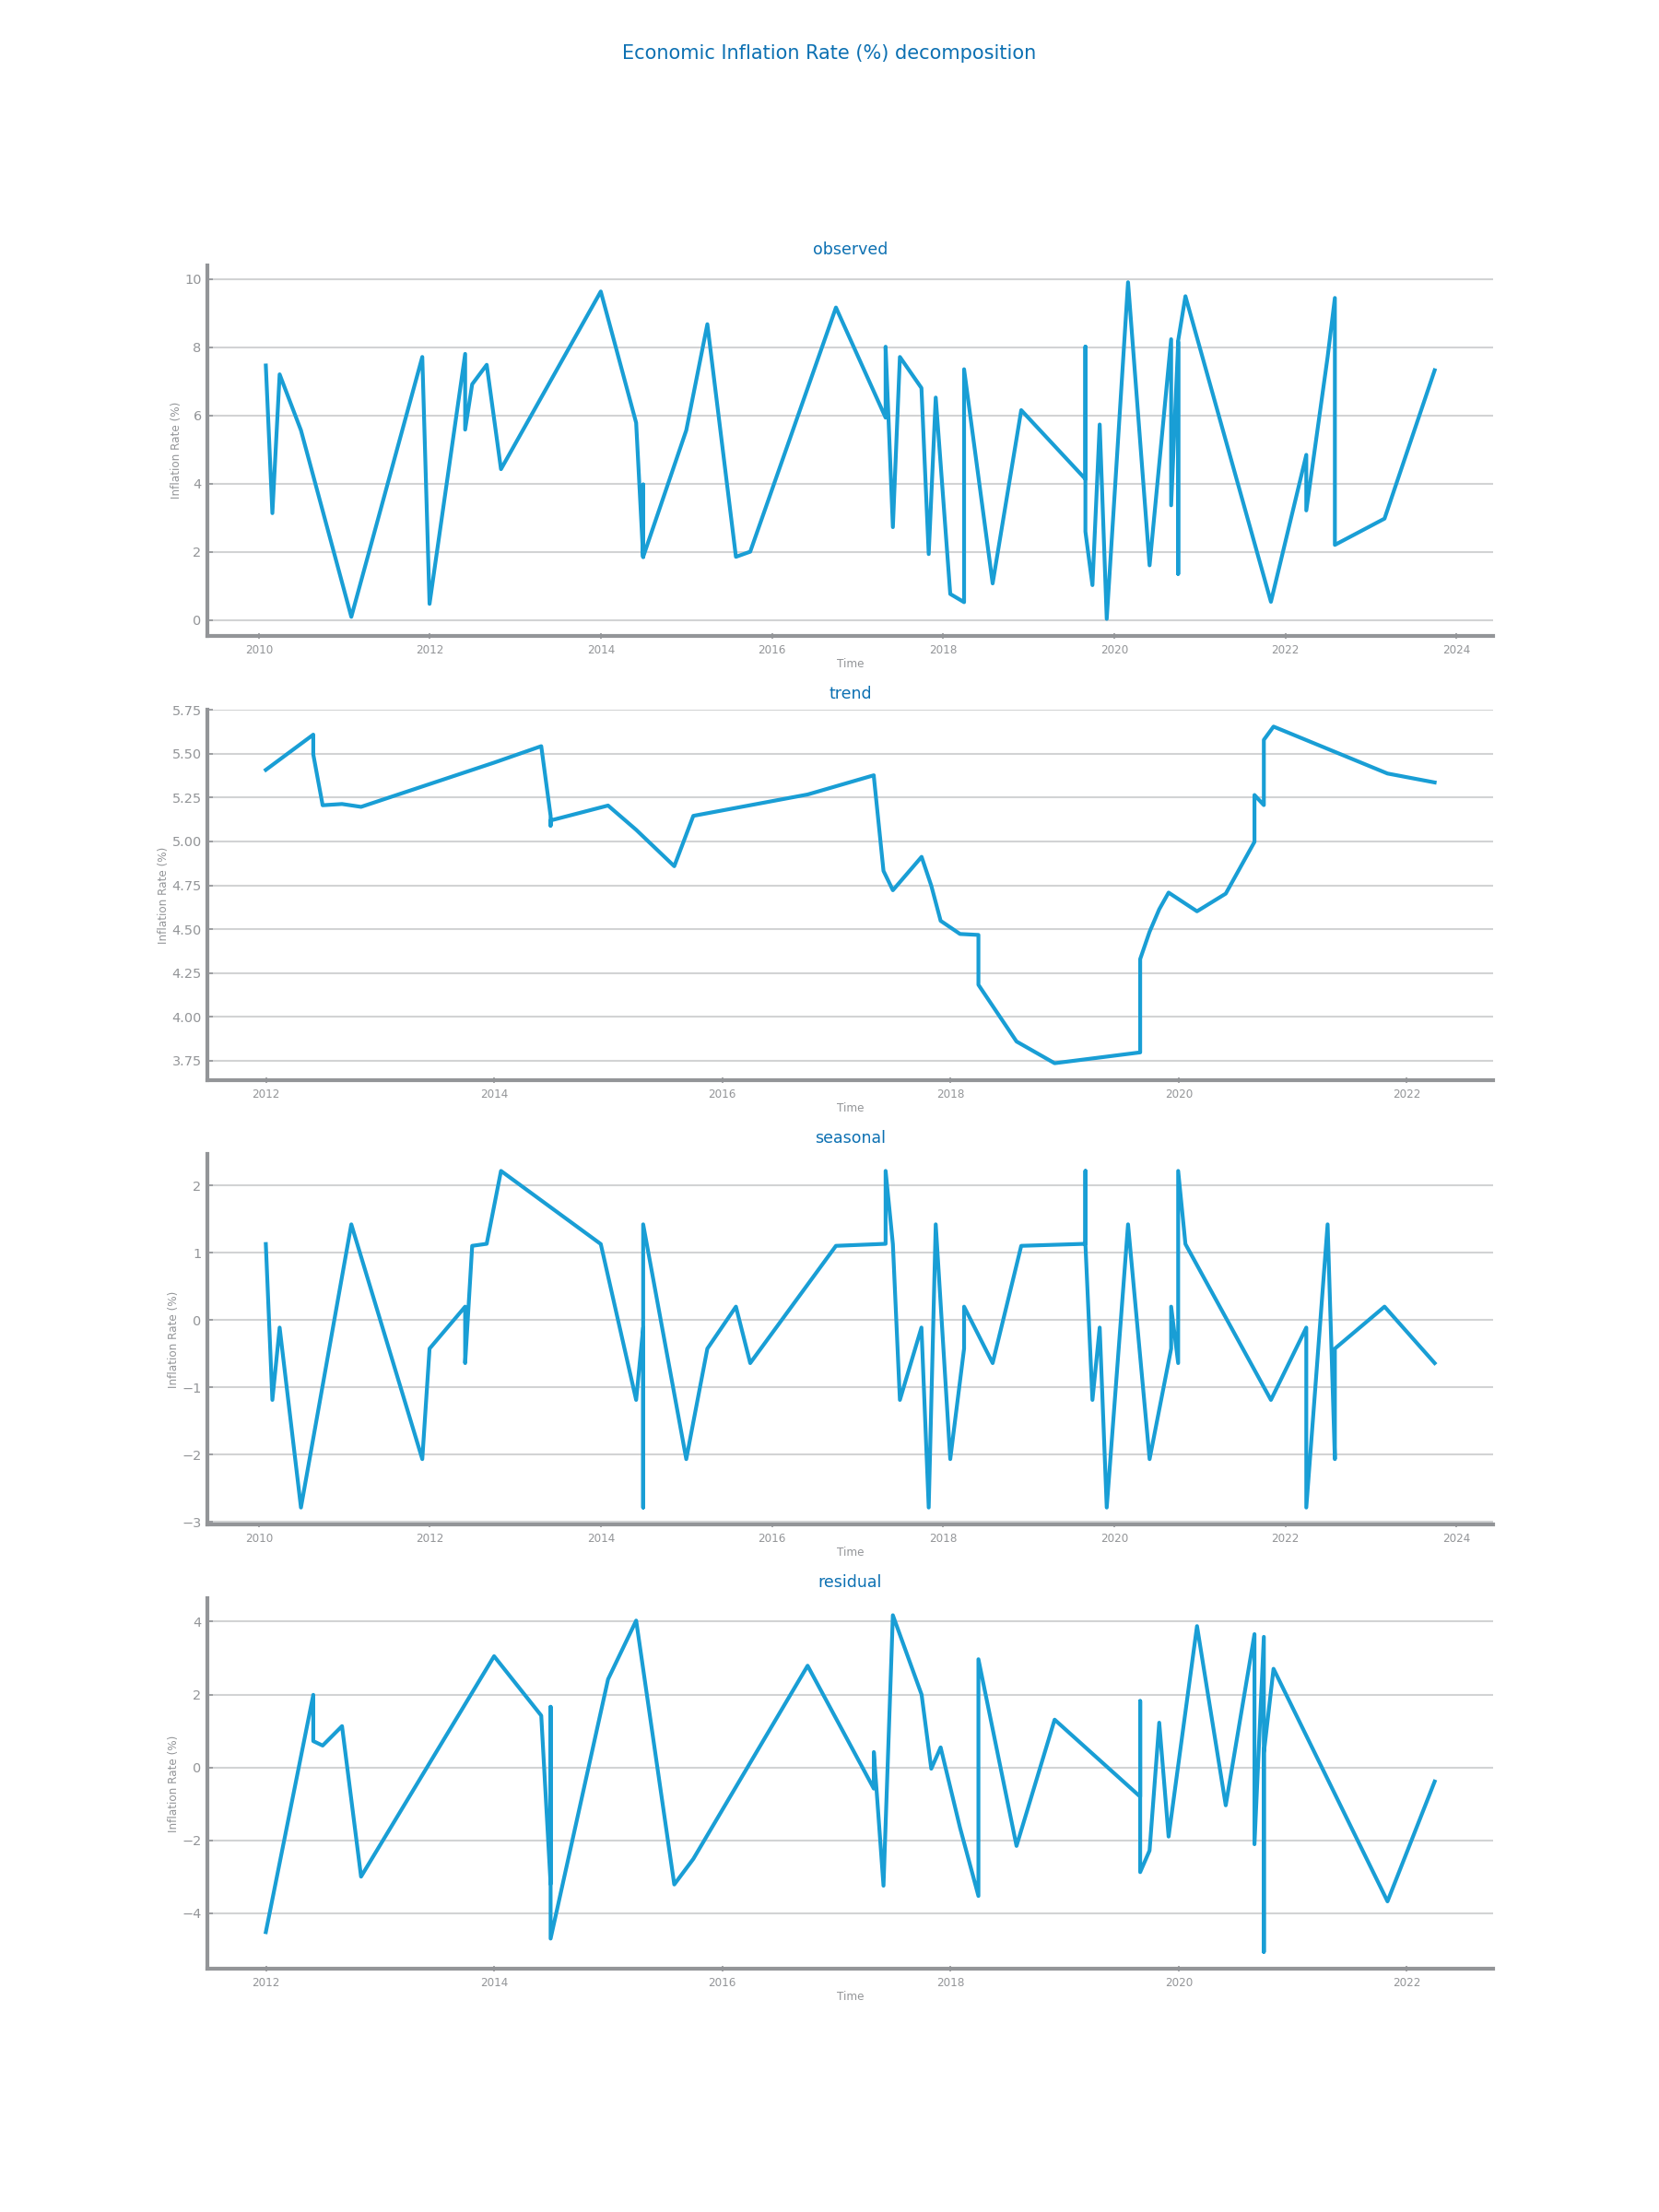
\includegraphics[width=0.9\textwidth]{Economic_seasonality.png}
\caption{Components study for time series 2}
\end{figure}


\begin{figure}[H]
\centering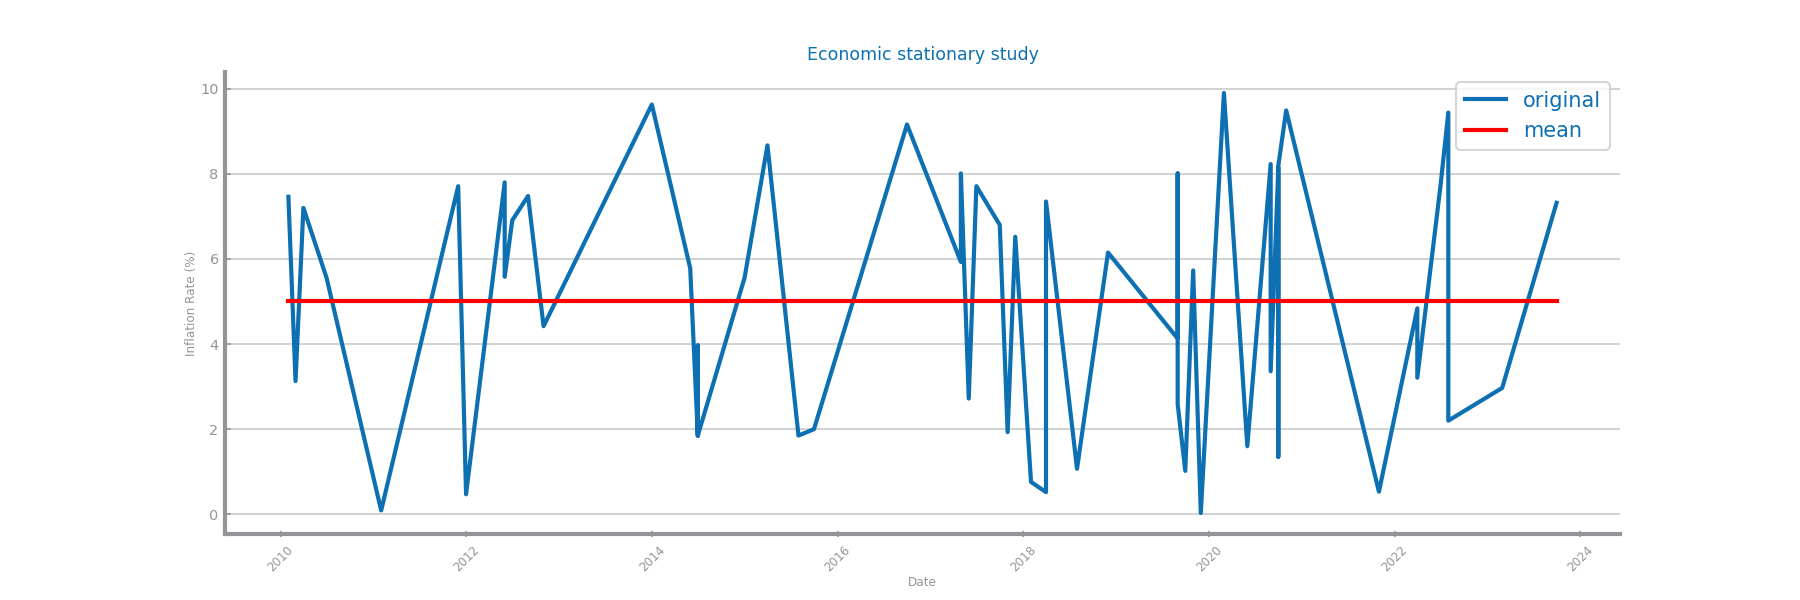
\includegraphics[width=0.9\textwidth]{Economic_stationarity_mean.png}
\caption{Stationarity study for time series 2}
\end{figure}

\section{DATA TRANSFORMATION}

\subsection*{\textit{Aggregation}}
\ctext[RGB]{190,190,190}{Shall describe the results of applying three different aggregations over both datasets, and identifying the granularity chosen to proceed.  \textbf{Shall not exceed 300 characters.}}

\begin{figure}[H]
\centering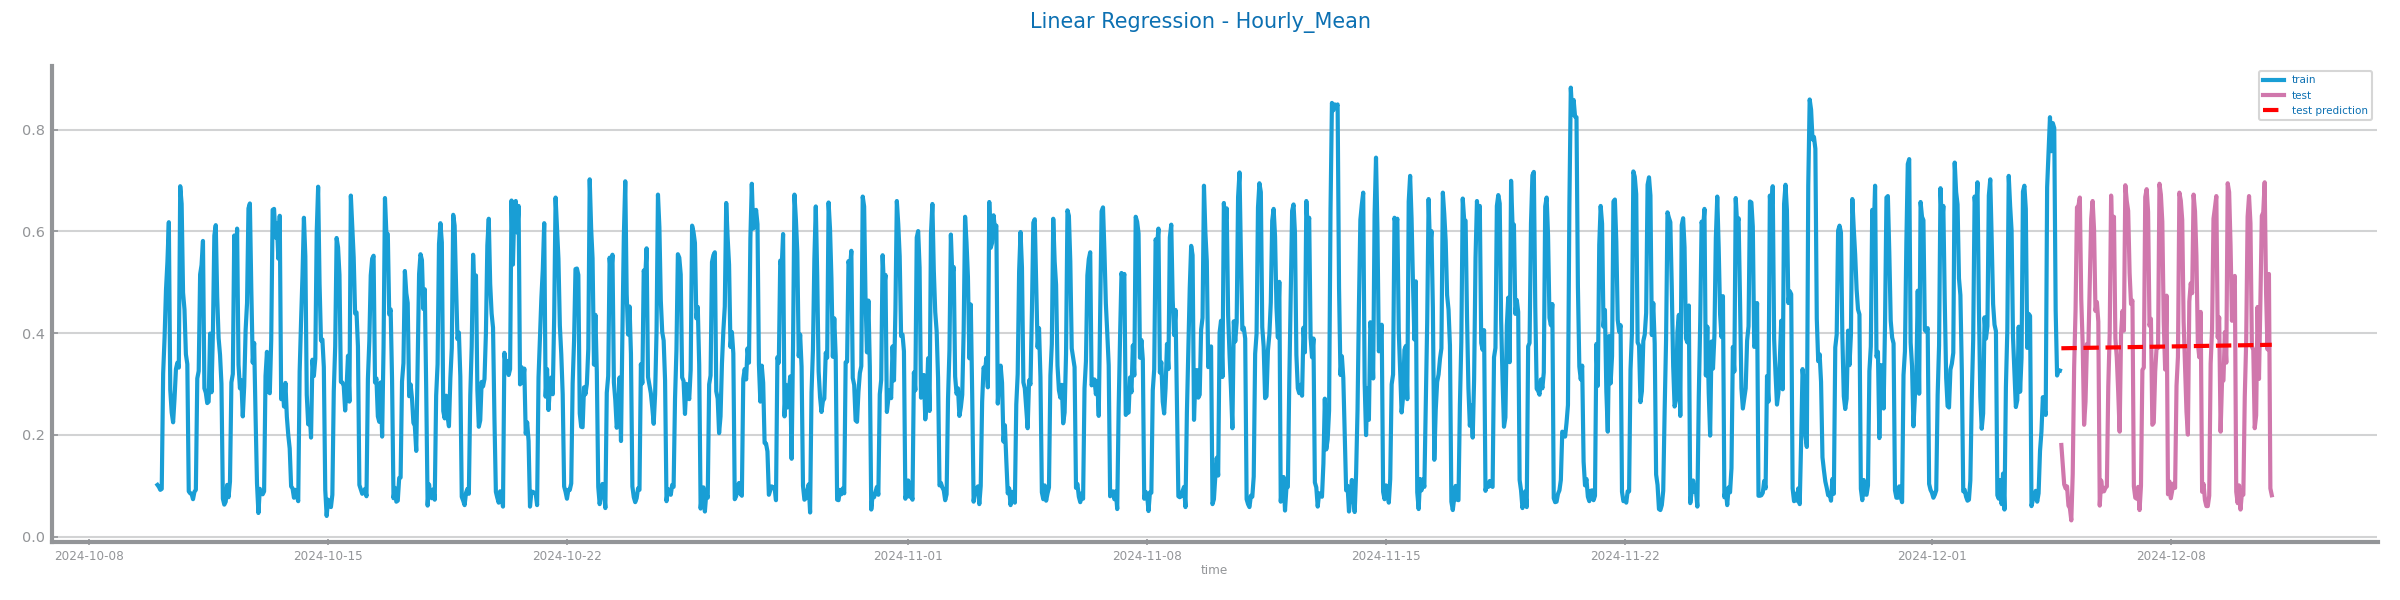
\includegraphics[width=0.9\textwidth]{traffic_agg_Hourly_Mean_lr.png}
\caption{Forecasting plots after different aggregations on time series 1}
\end{figure}

\begin{figure}[H]
\centering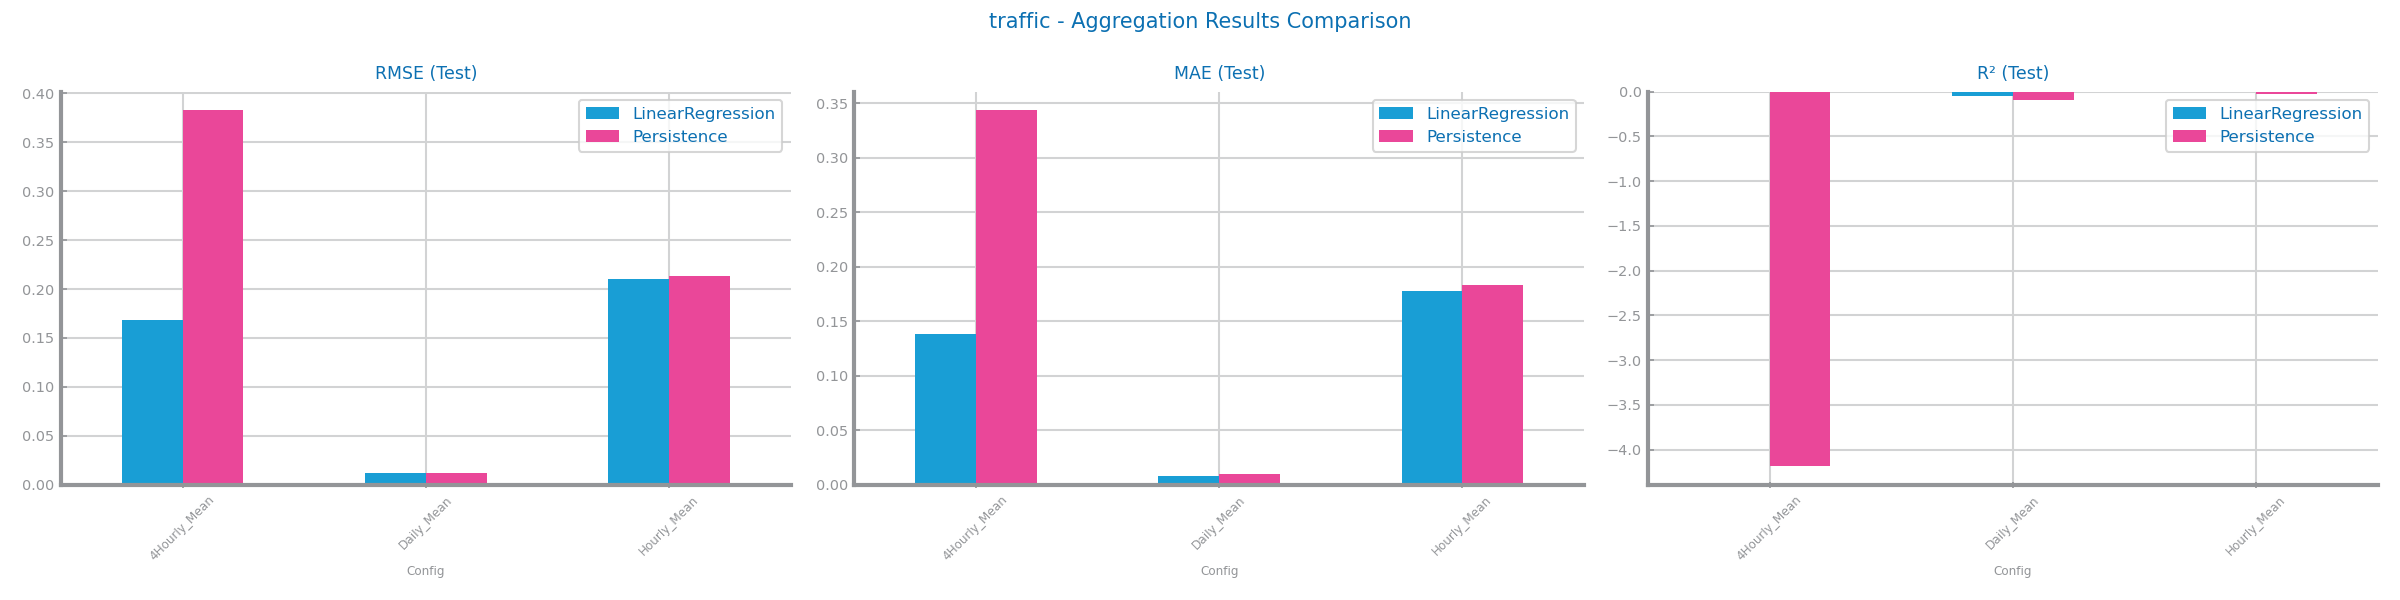
\includegraphics[width=0.9\textwidth]{traffic_aggregation_comparison_chart.png}
\caption{Forecasting results after different aggregations on time series 1}
\end{figure}

\begin{figure}[H]
\centering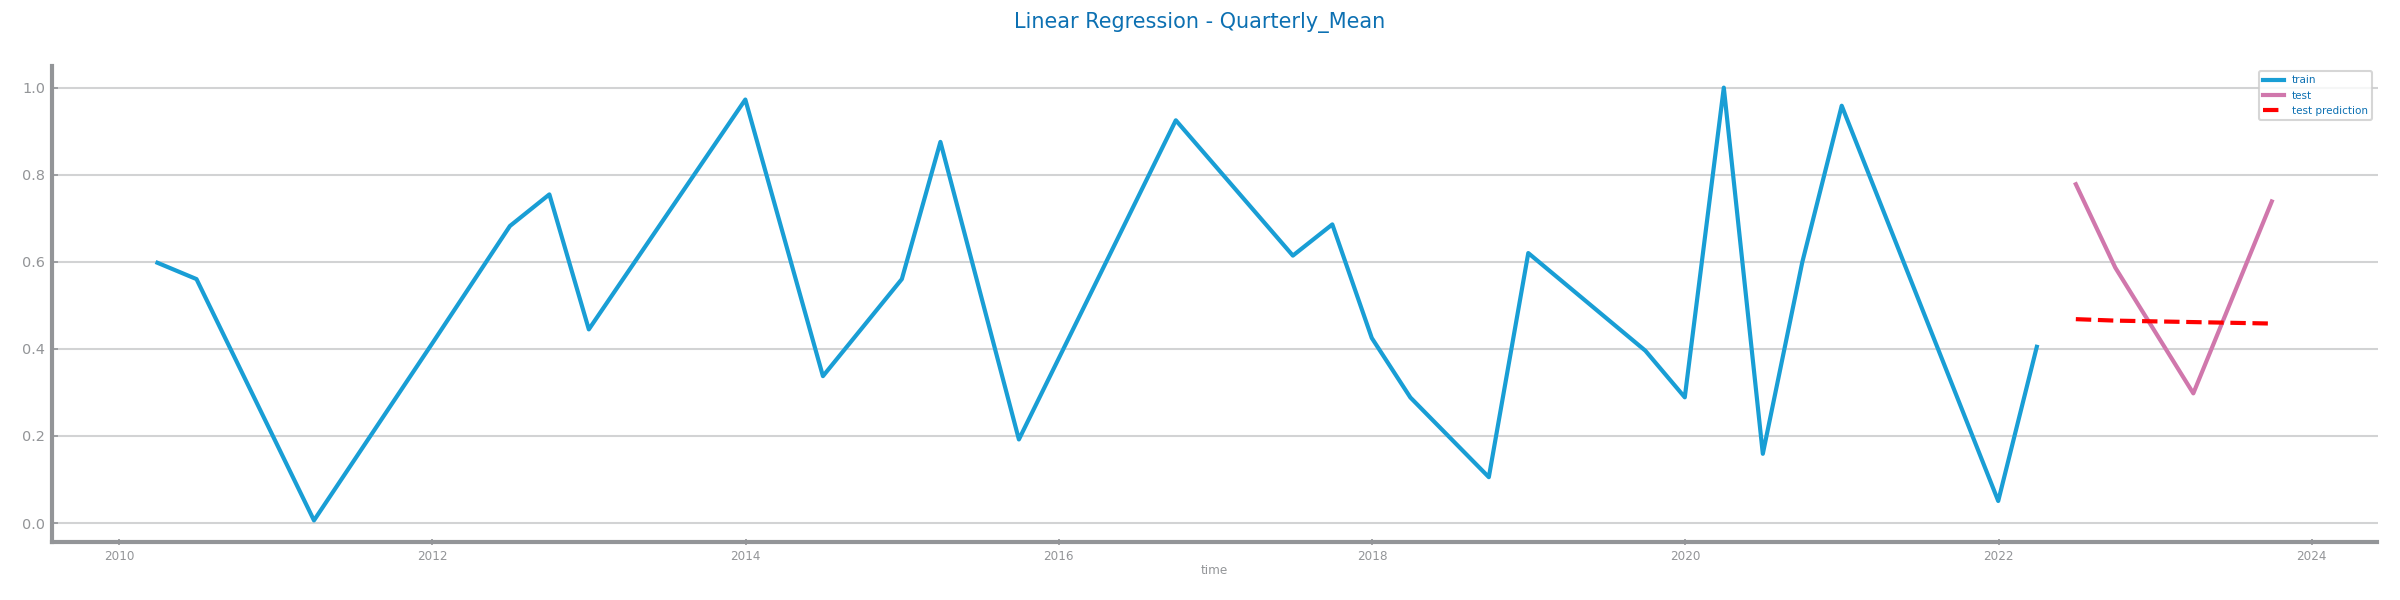
\includegraphics[width=0.9\textwidth]{economic_usa_agg_Quarterly_Mean_lr.png}
\caption{Forecasting plots after different aggregations on time series 2}
\end{figure}

\begin{figure}[H]
\centering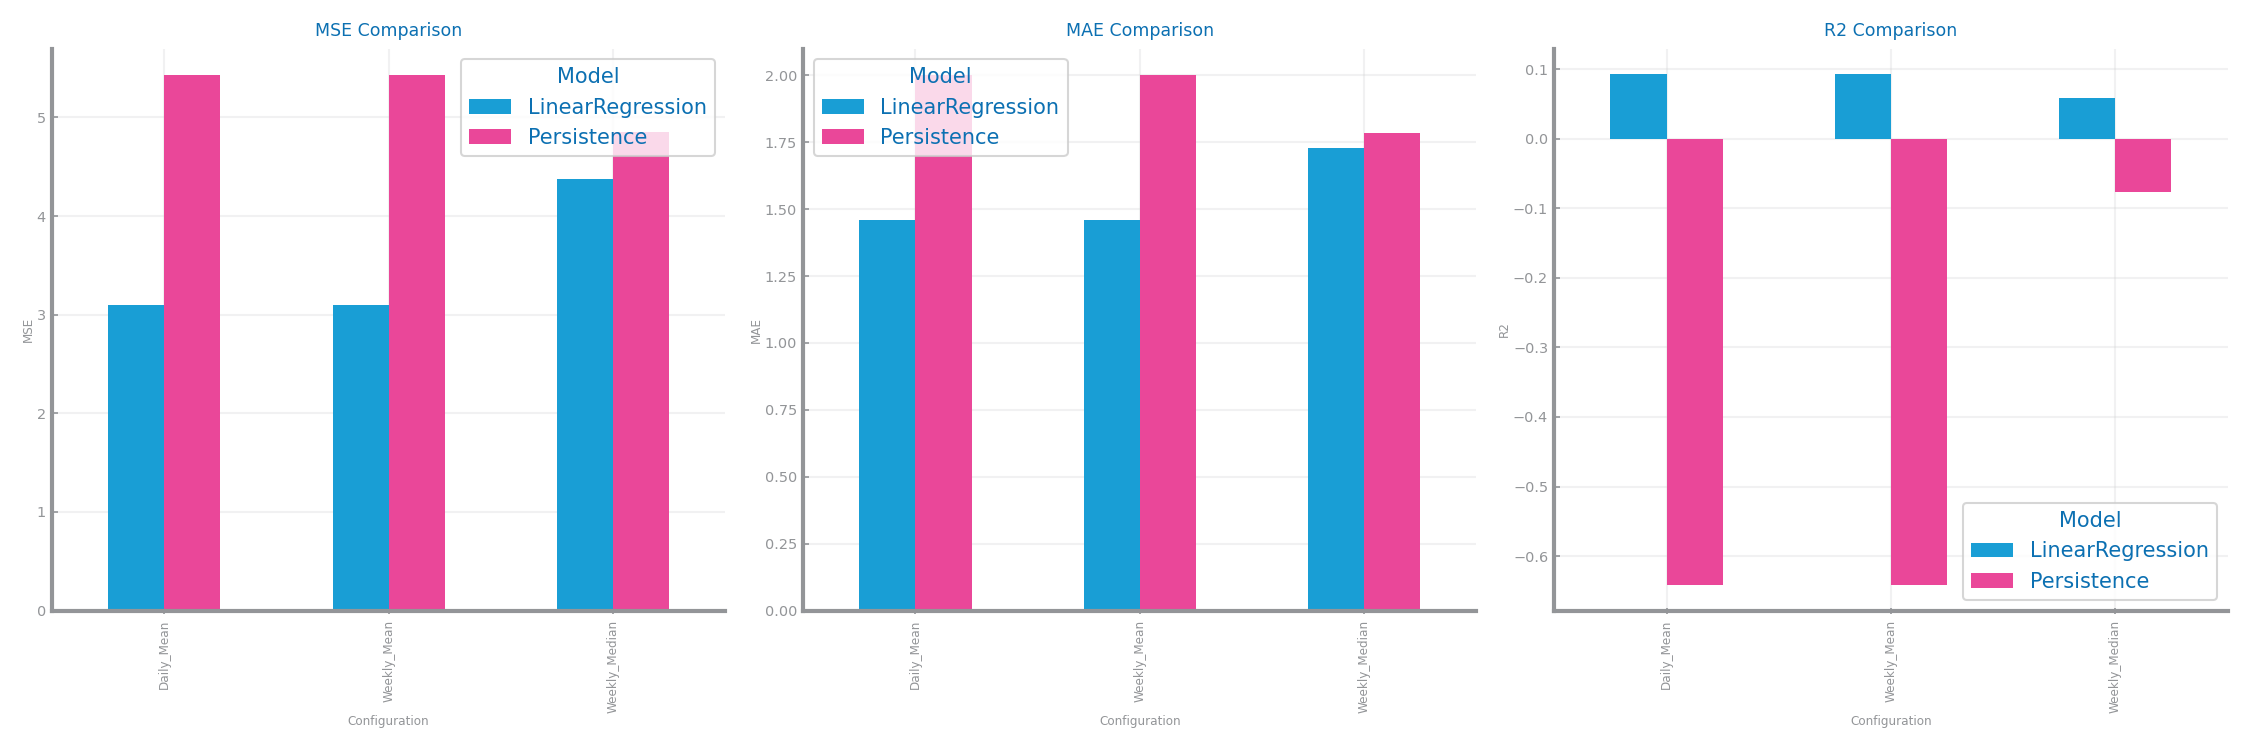
\includegraphics[width=0.9\textwidth]{economic_aggregation_summary.png}
\caption{Forecasting results after different aggregations on time series 2}
\end{figure}

\subsection*{\textit{Smoothing}}
\ctext[RGB]{190,190,190}{Shall describe the results of applying smoothing transformations over both datasets, and identifying the best result to proceed.  \textbf{Shall not exceed 300 characters.}}

\begin{figure}[H]
\centering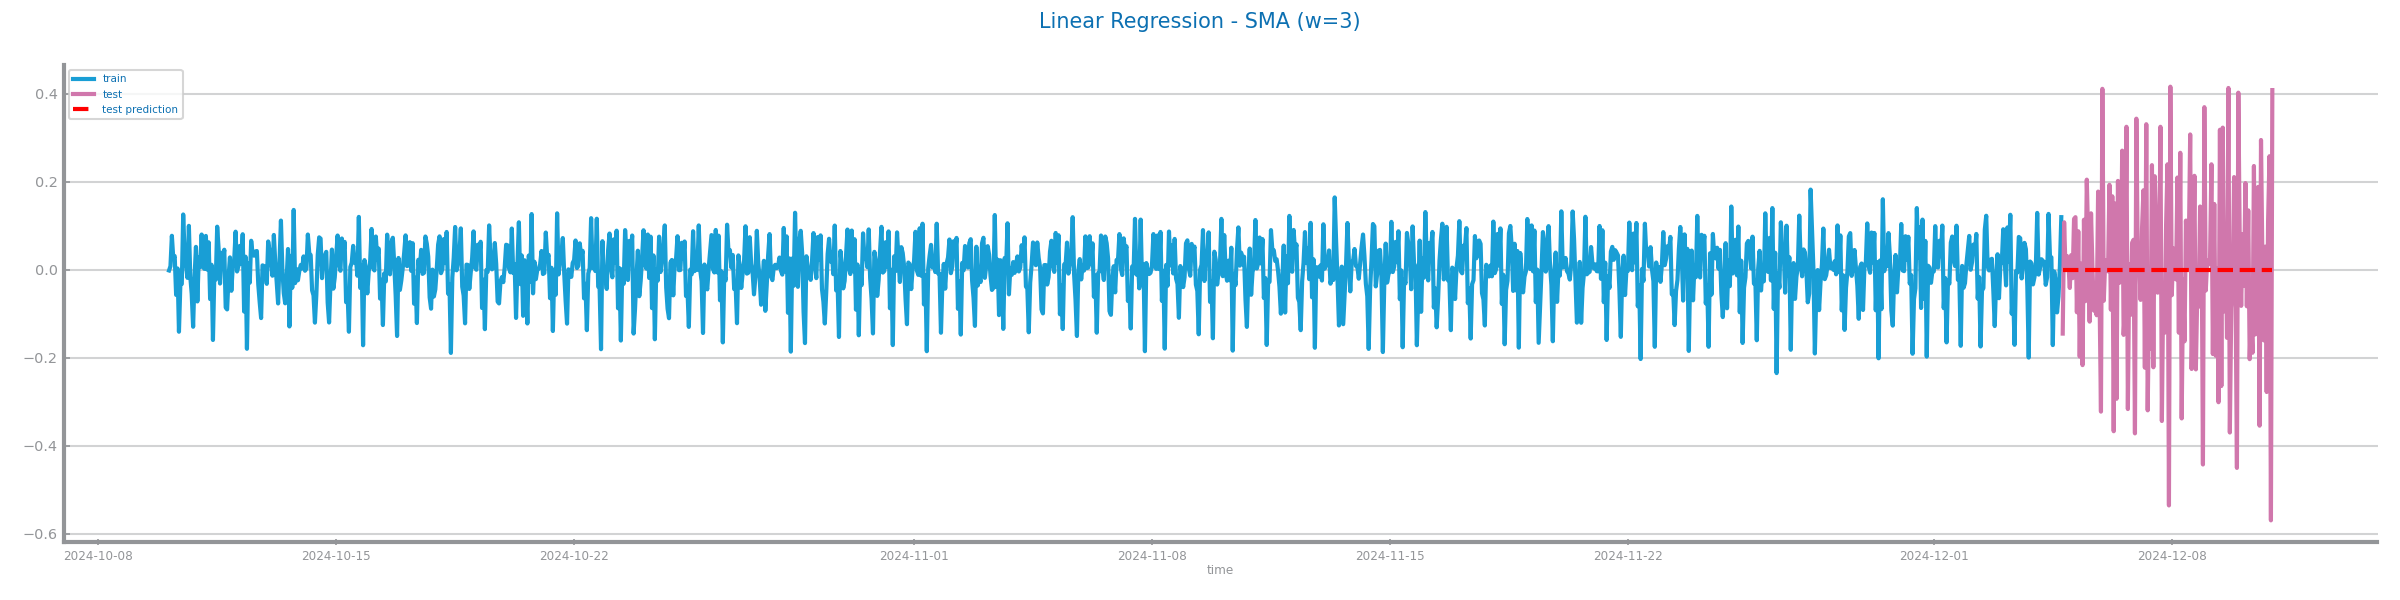
\includegraphics[width=0.9\textwidth]{traffic_lr_SMA_w3.png}
\caption{Forecasting plots after different smoothing parameterisations on time series 1}
\end{figure}

\begin{figure}[H]
\centering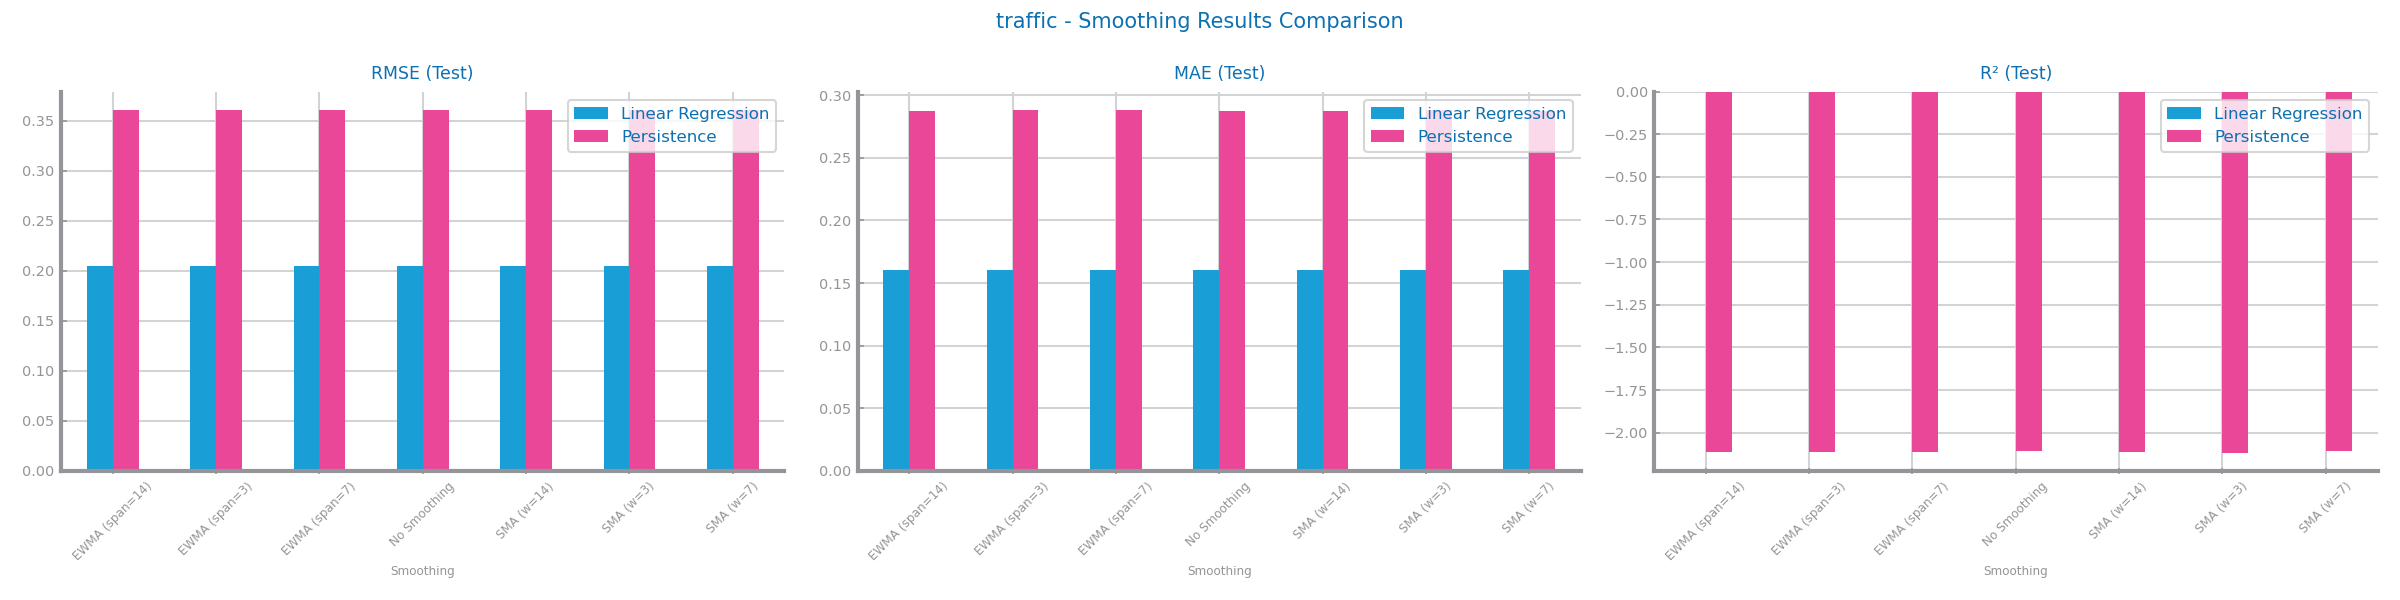
\includegraphics[width=0.9\textwidth]{traffic_smoothing_comparison_chart.png}
\caption{Forecasting results after different smoothing parameterisations on time series 1}
\end{figure}

\begin{figure}[H]
\centering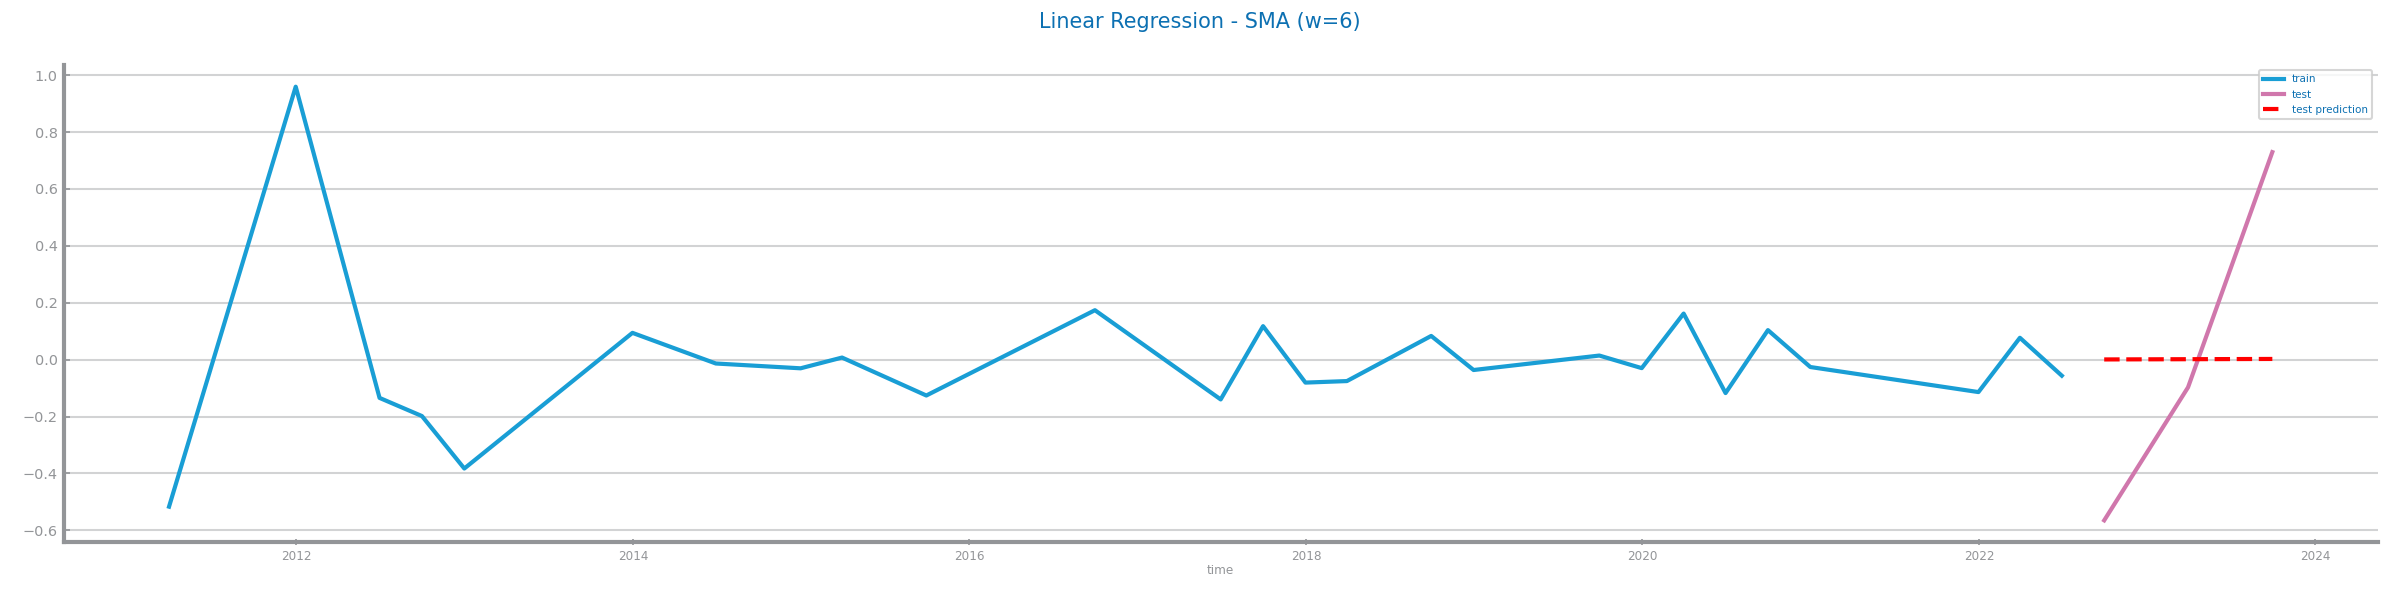
\includegraphics[width=0.9\textwidth]{economic_usa_lr_SMA_w6.png}
\caption{Forecasting plots after different smoothing parameterisations on time series 2}
\end{figure}

\begin{figure}[H]
\centering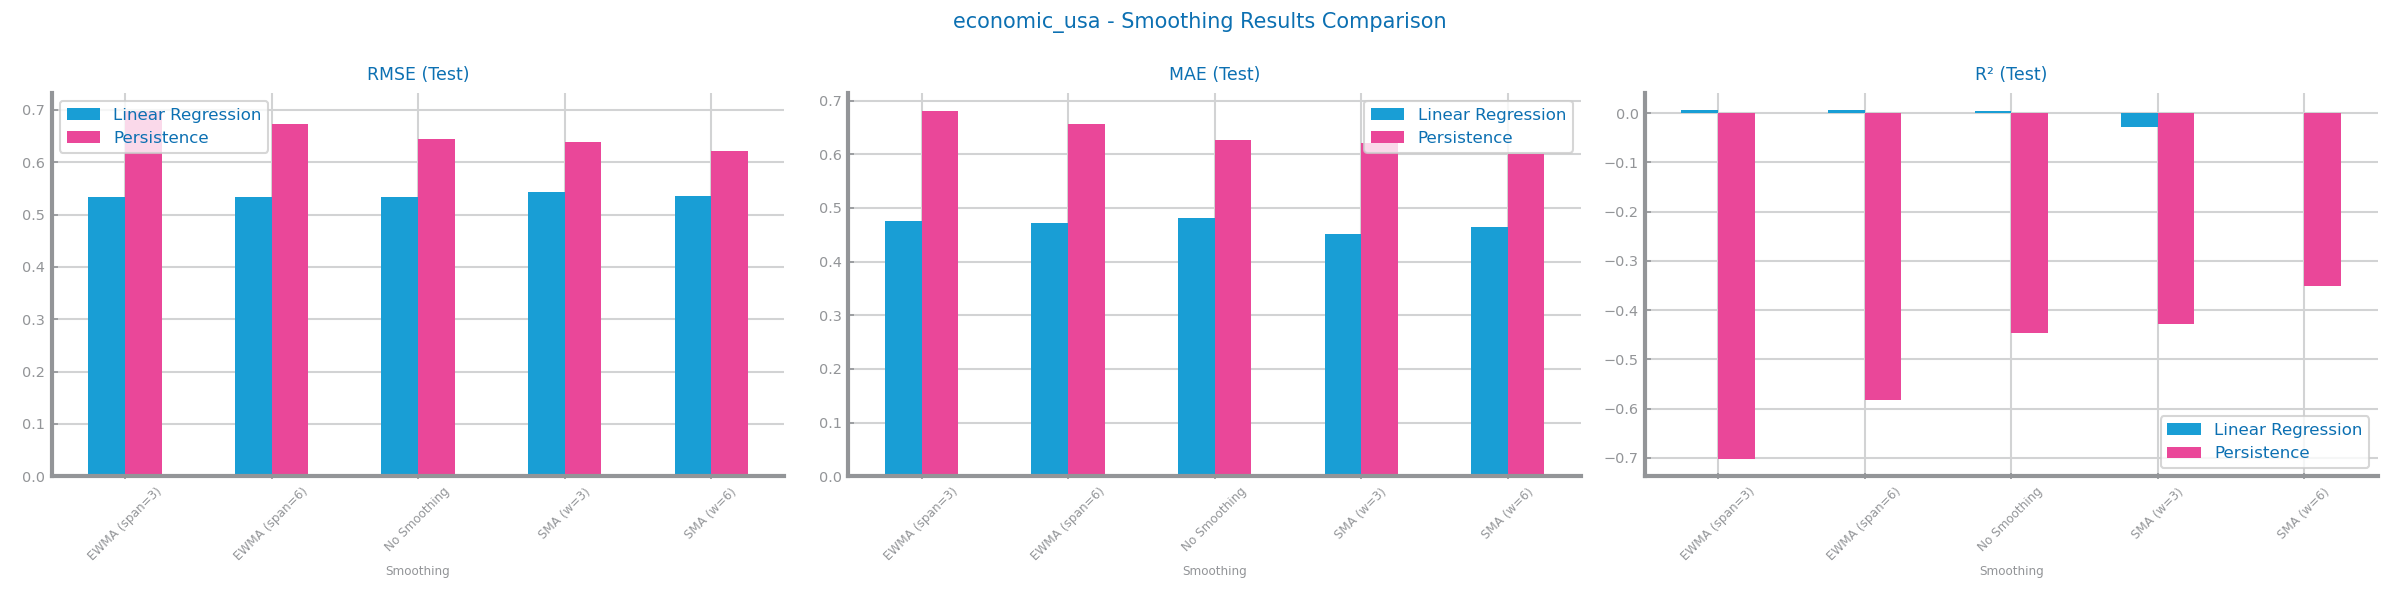
\includegraphics[width=0.9\textwidth]{economic_usa_smoothing_comparison_chart.png}
\caption{Forecasting results after different smoothing parameterisations on time series 2}
\end{figure}

\subsection*{\textit{Differentiation}}
\ctext[RGB]{190,190,190}{Shall describe the results of applying two consecutive differentiation of both datasets, and identifying the best result to proceed.  \textbf{Shall not exceed 300 characters.}}

\begin{figure}[H]
\centering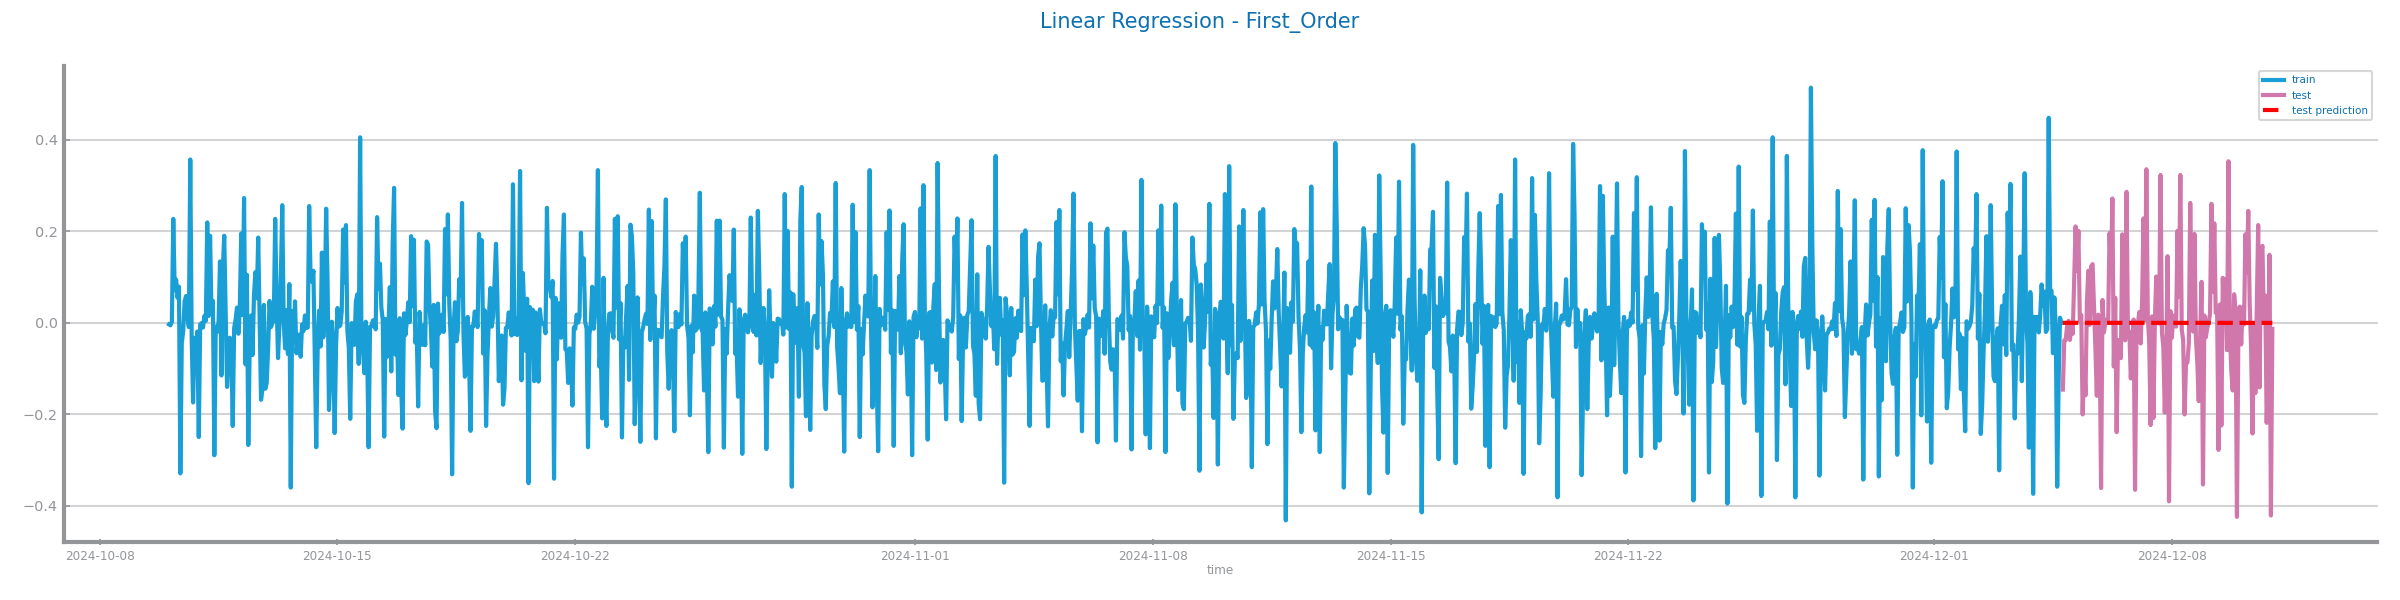
\includegraphics[width=0.9\textwidth]{traffic_diff_First_Order_lr.png}
\caption{Forecasting plots after first and second differentiation of time series 1}
\end{figure}

\begin{figure}[H]
\centering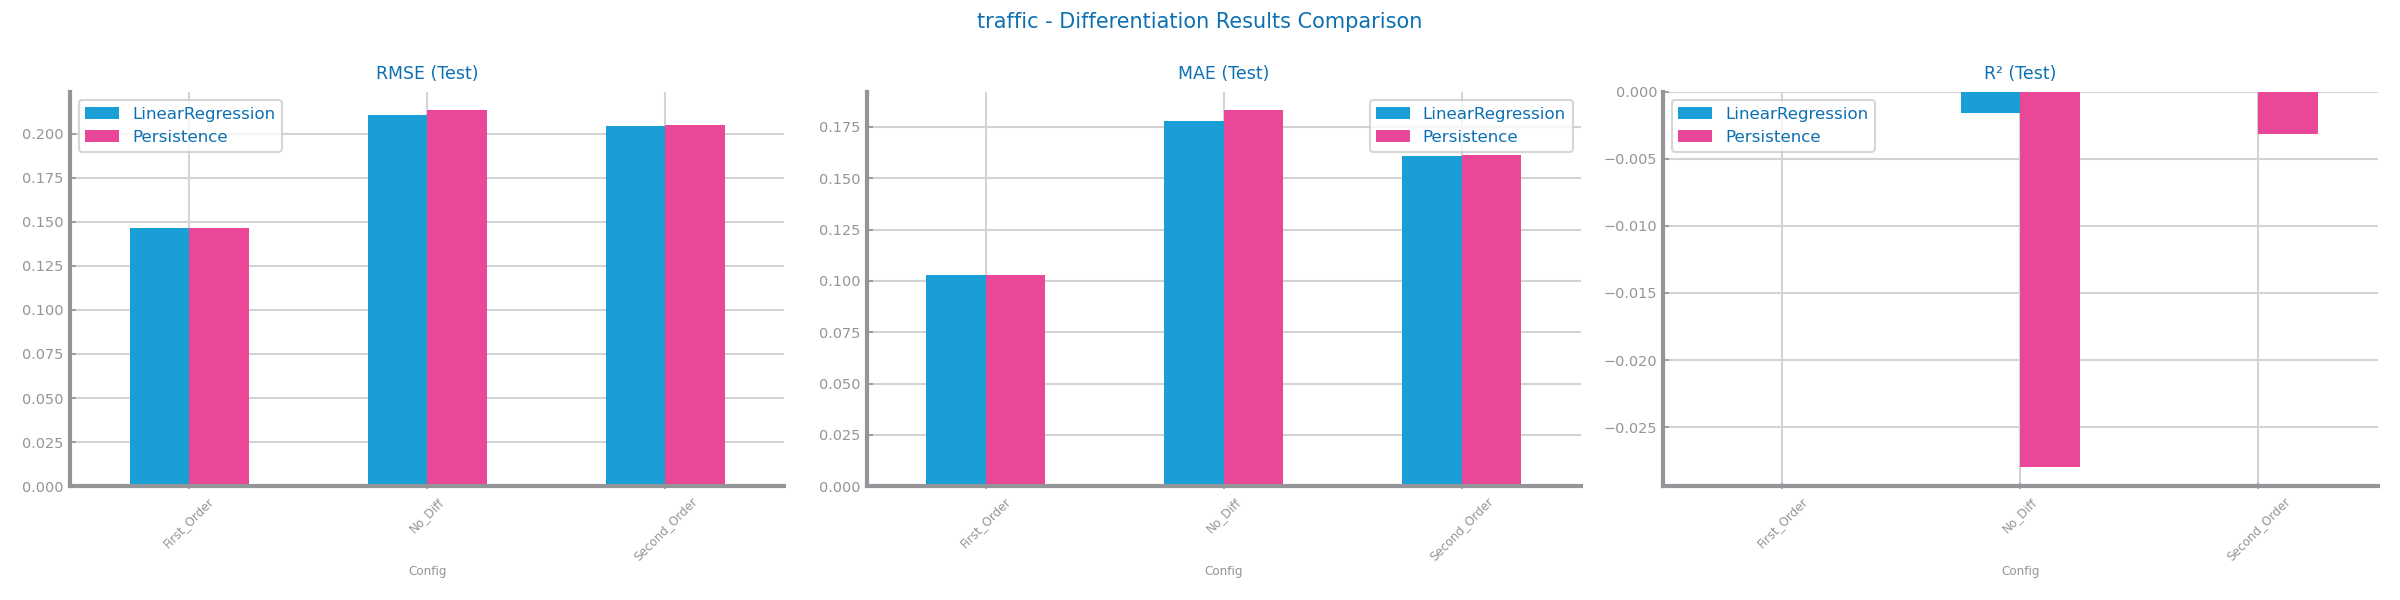
\includegraphics[width=0.9\textwidth]{traffic_differentiation_comparison_chart.png}
\caption{Forecasting results after first and second differentiation of time series 1}
\end{figure}

\begin{figure}[H]
\centering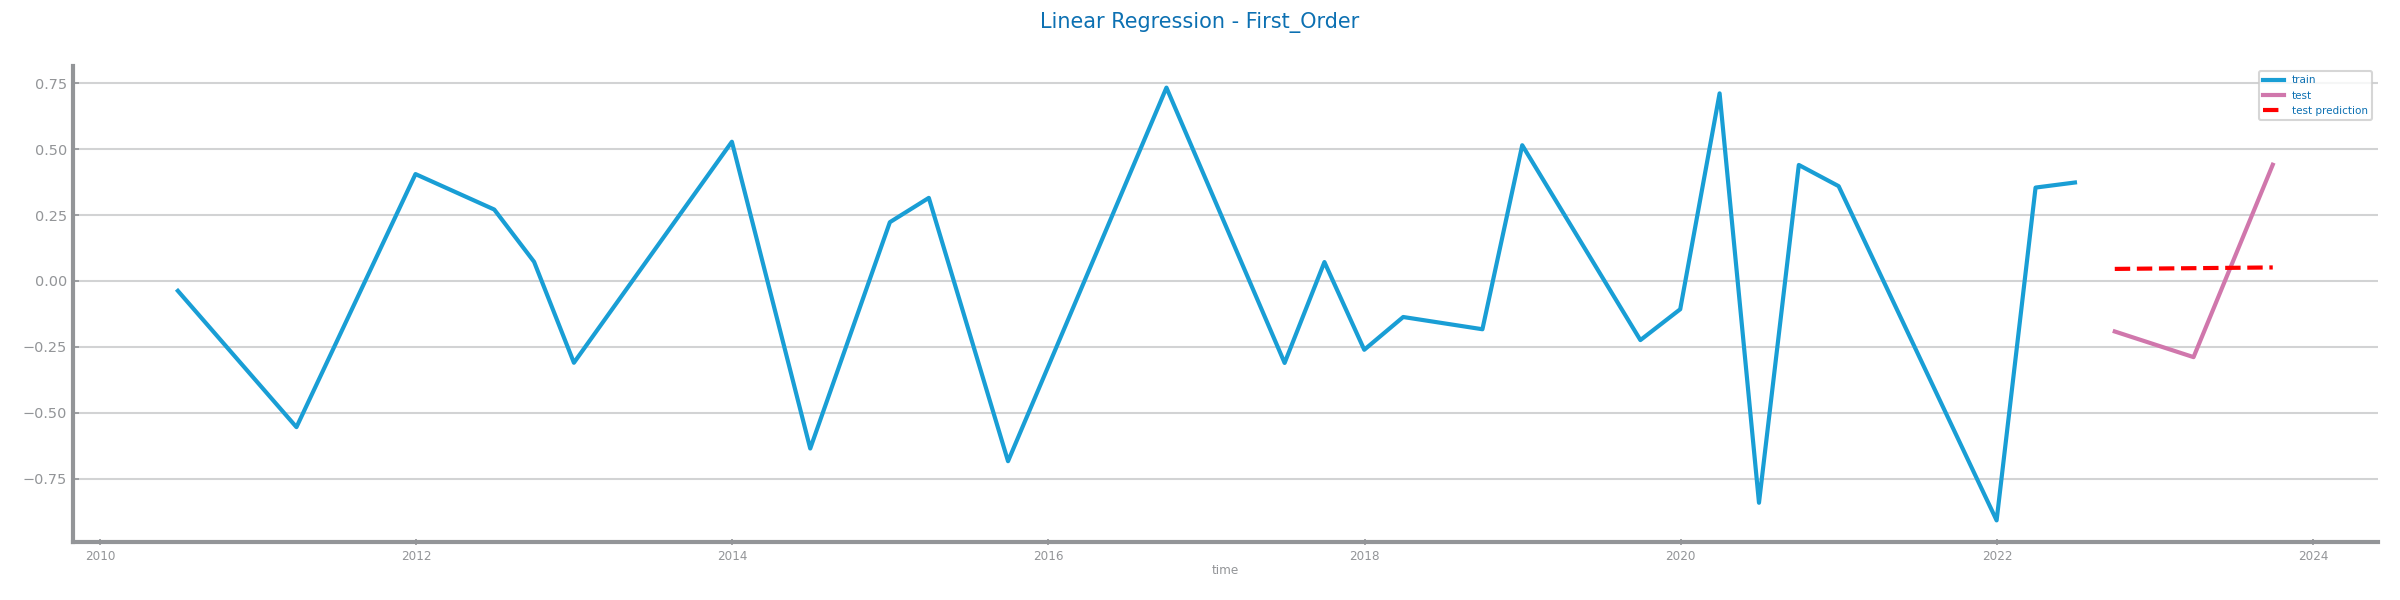
\includegraphics[width=0.9\textwidth]{economic_usa_diff_First_Order_lr.png}
\caption{Forecasting plots after first and second differentiation of time series 2}
\end{figure}

\begin{figure}[H]
\centering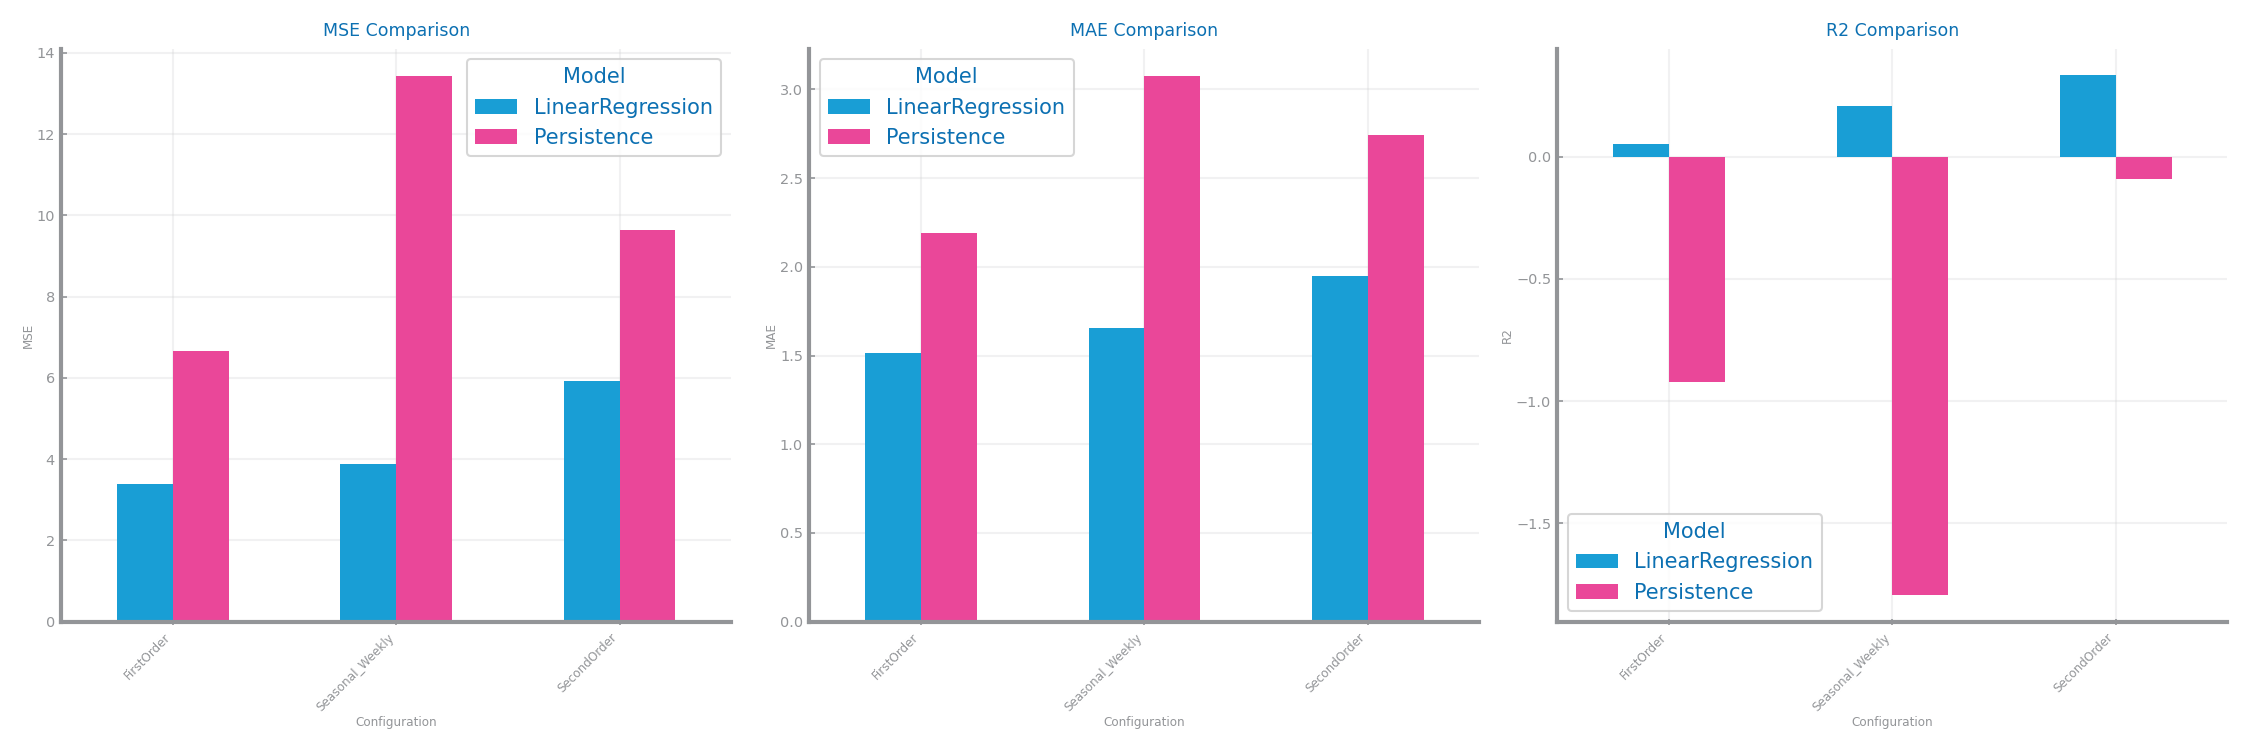
\includegraphics[width=0.9\textwidth]{economic_differentiation_summary.png}
\caption{Forecasting results after first and second differentiation of time series 2}
\end{figure}

\subsection*{\textit{Other transformations (optional)}}
\ctext[RGB]{190,190,190}{Shall describe the results of applying other transformations over both datasets, and identifying the best result to proceed.  \textbf{Shall not exceed 500 characters.}}

\begin{figure}[H]
%\centering\includegraphics[width=0.9\textwidth]{}
\caption{Forecasting plots after applying other transformations over time series 1}
\end{figure}

\begin{figure}[H]
%\centering\includegraphics[width=0.9\textwidth]{}
\caption{Forecasting results after applying other transformations over time series 1}
\end{figure}

\begin{figure}[H]
%\centering\includegraphics[width=0.9\textwidth]{}
\caption{Forecasting plots after applying other transformations over time series 2}
\end{figure}

\begin{figure}[H]
%\centering\includegraphics[width=0.9\textwidth]{}
\caption{FForecasting results after applying other transformations over time series 2}
\end{figure}

\section{MODELS' EVALUATION}
\ctext[RGB]{190,190,190}{Shall be used to summarise the transformations done over the original time series.  \textbf{Shall not exceed 500 characters.}}

\subsection*{\textit{Simple Average Model}}
\ctext[RGB]{190,190,190}{Shall be used to present the results achieved through the simple average model.  \textbf{Shall not exceed 200 characters.}}

\begin{figure}[H]
\centering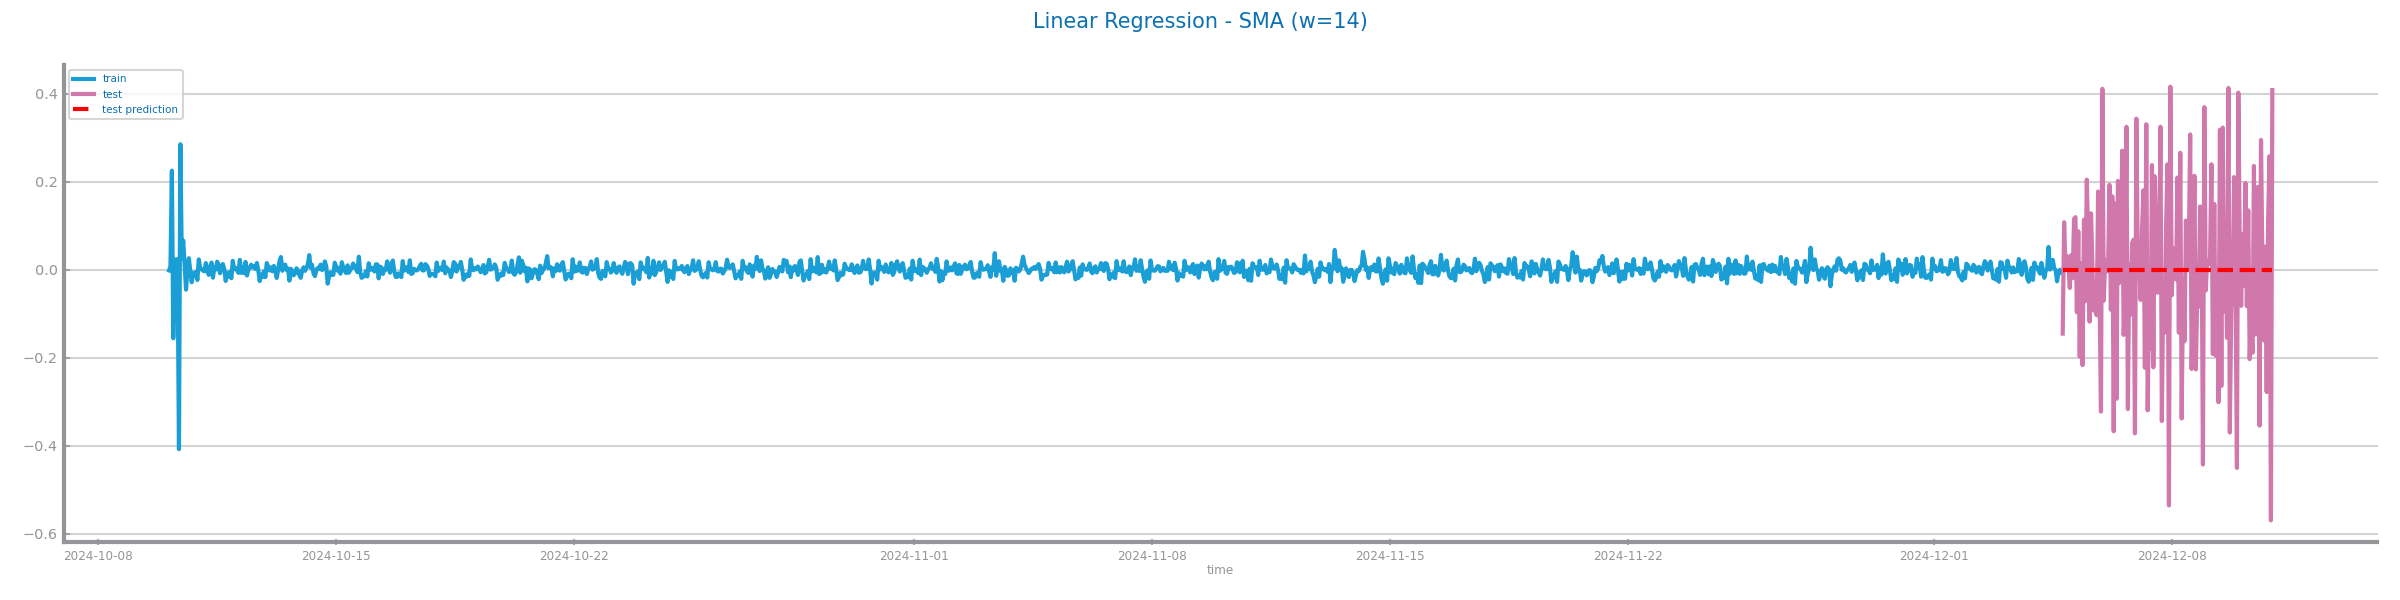
\includegraphics[width=0.9\textwidth]{traffic_lr_SMA_w14.png}
\caption{Forecasting plots obtained with Simple Average model over time series 1}
\end{figure}

\begin{figure}[H]
\centering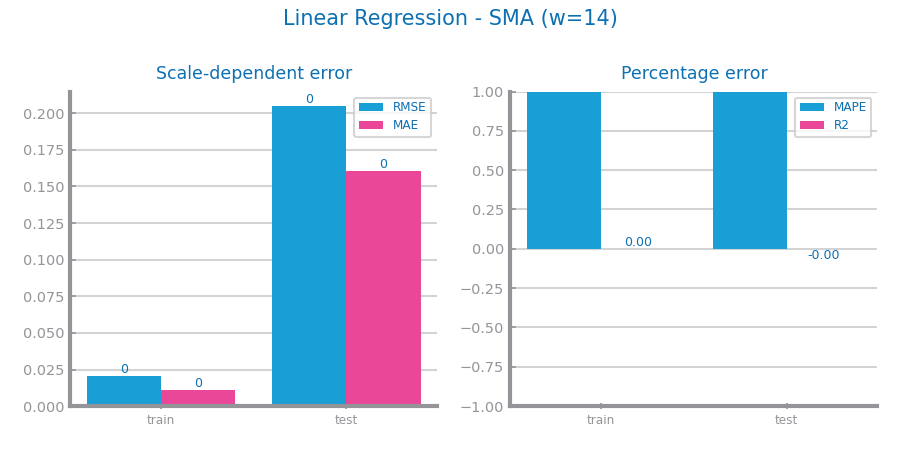
\includegraphics[width=0.9\textwidth]{traffic_lr_eval_SMA_w14.png}
\caption{Forecasting results obtained with Simple Average model over time series 1}
\end{figure}

\begin{figure}[H]
\centering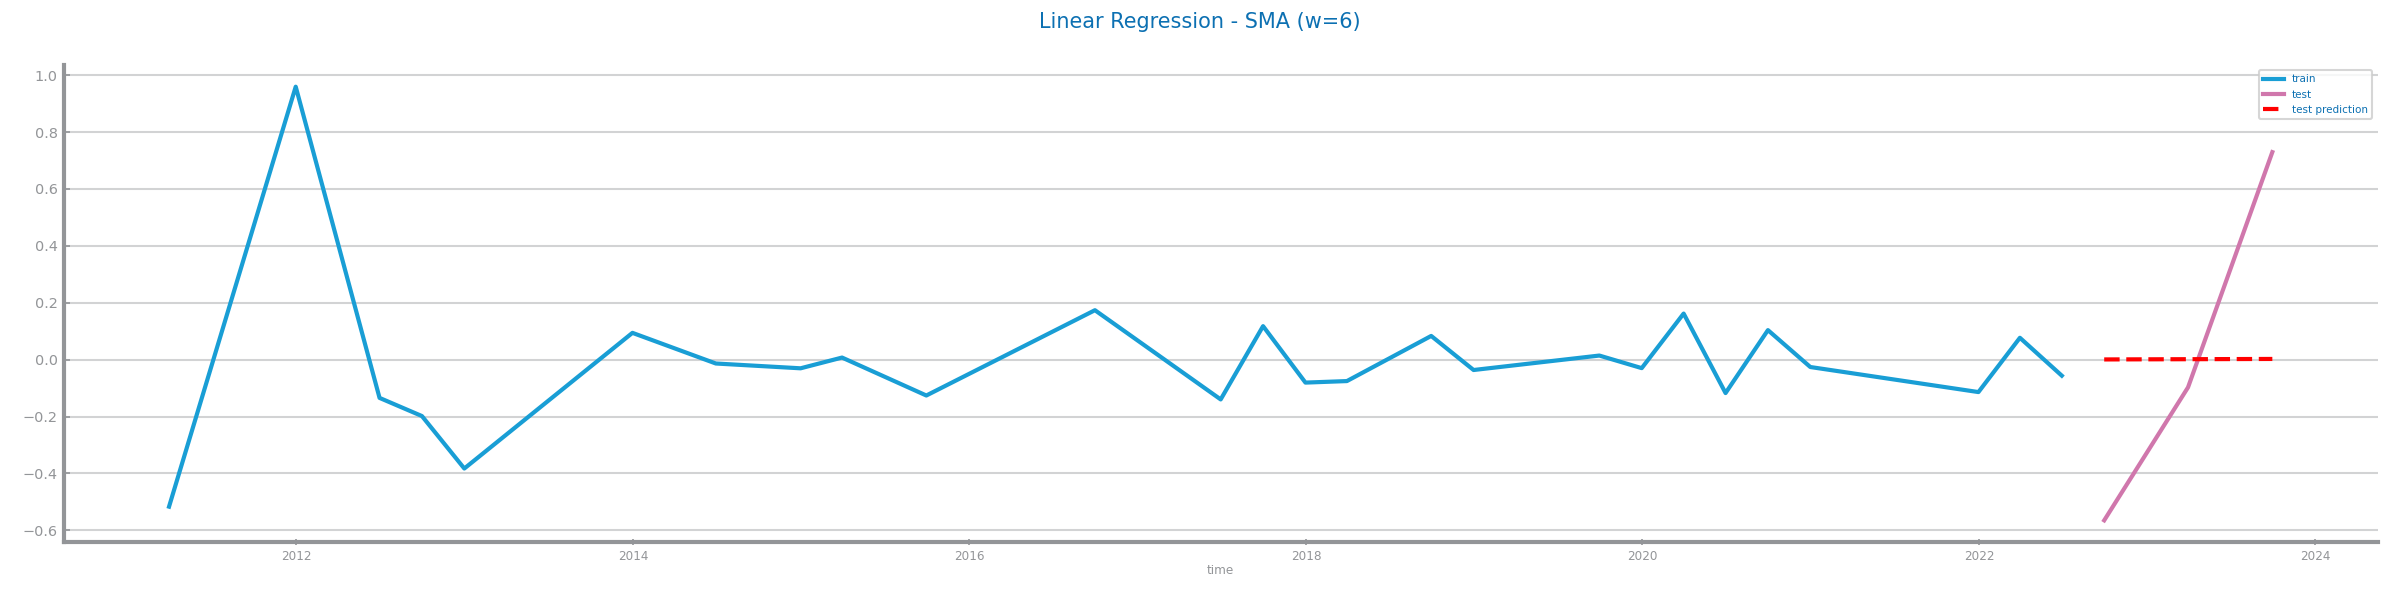
\includegraphics[width=0.9\textwidth]{economic_usa_lr_SMA_w6.png}
\caption{Forecasting plots obtained with Simple Average model over time series 2}
\end{figure}

\begin{figure}[H]
\centering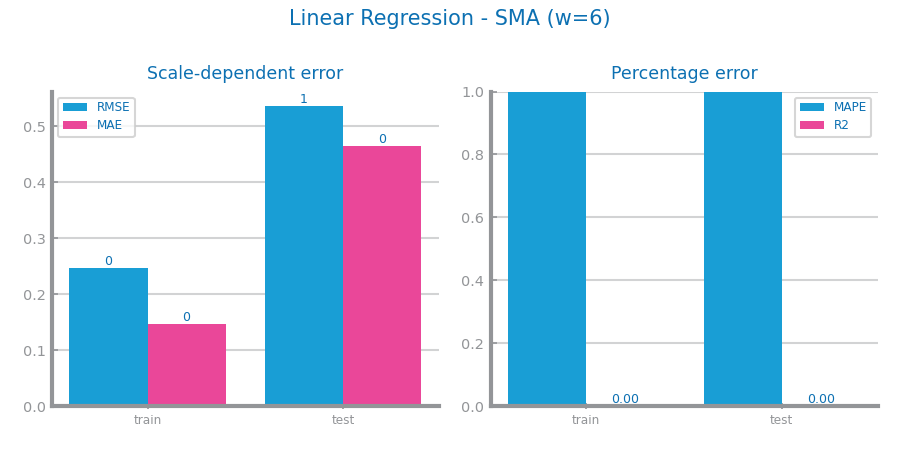
\includegraphics[width=0.9\textwidth]{economic_usa_lr_eval_SMA_w6.png}
\caption{Forecasting results obtained with Simple Average model over time series 2}
\end{figure}

\subsection*{\textit{Persistence Model}}
\ctext[RGB]{190,190,190}{Shall be used to present the results achieved through the persistence model.  \textbf{Shall not exceed 500 characters.}}

\begin{figure}[H]
\centering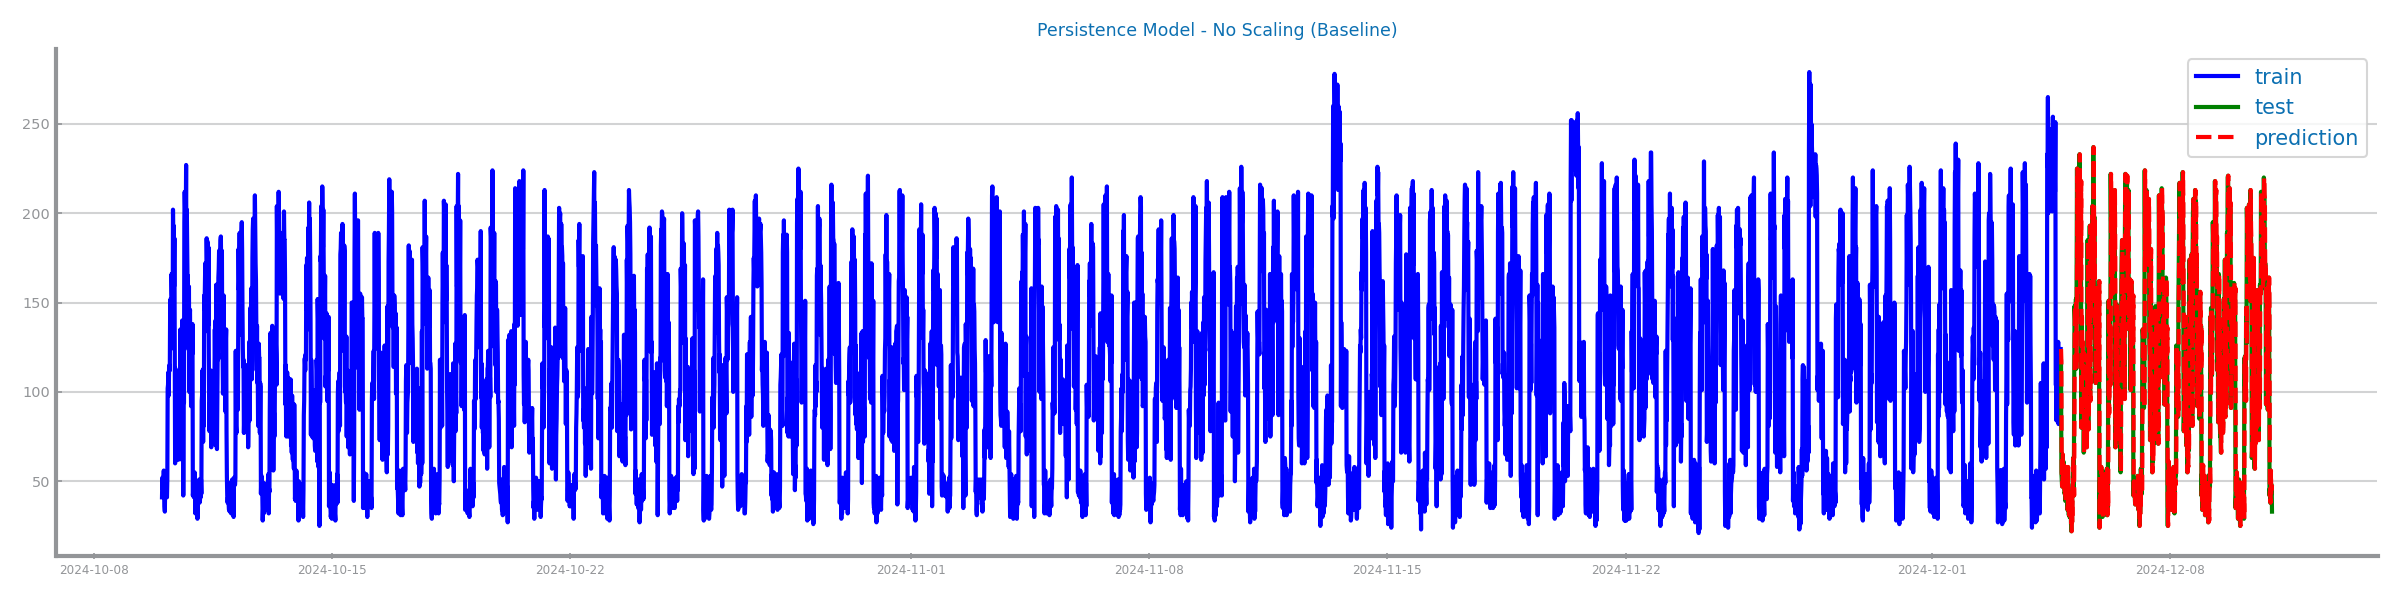
\includegraphics[width=0.9\textwidth]{traffic_persistence_none.png}
\caption{Forecasting plots obtained with Persistence model (long term) over time series 1}
\end{figure}

\begin{figure}[H]
\centering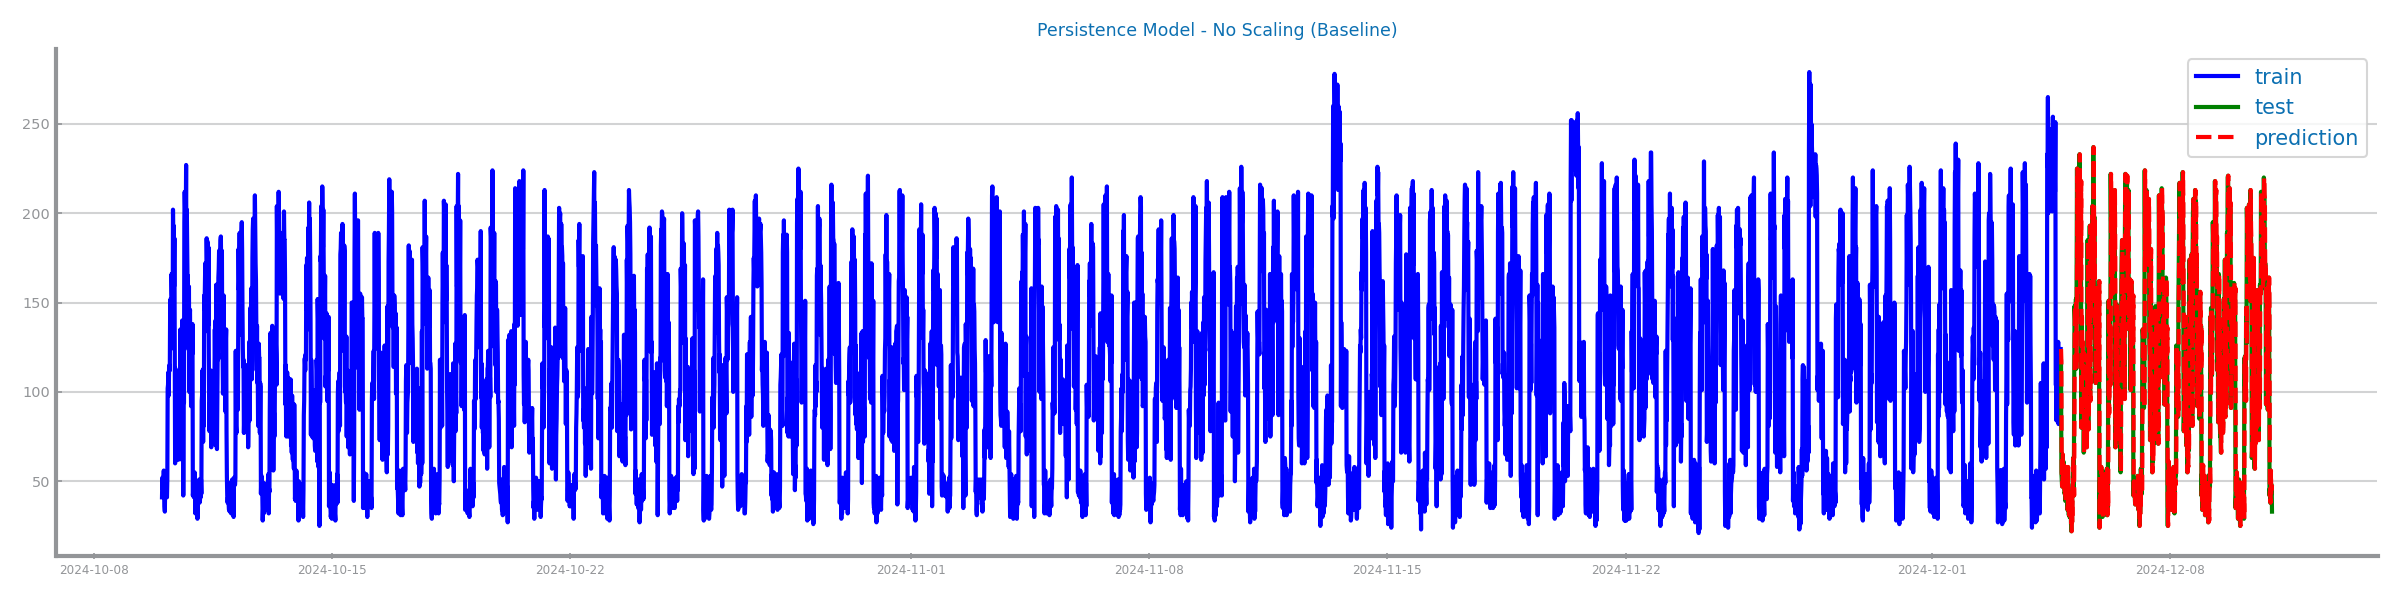
\includegraphics[width=0.9\textwidth]{traffic_persistence_none.png}
\caption{Forecasting plots obtained with Persistence model (one-set-behind) over time series 1}
\end{figure}

\begin{figure}[H]
\centering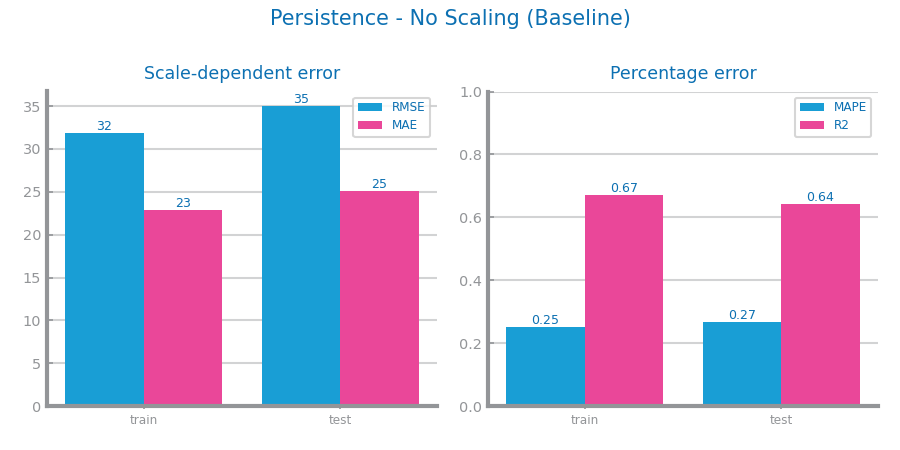
\includegraphics[width=0.9\textwidth]{traffic_persistence_eval_none.png}
\caption{Forecasting results obtained with Persistence model in both situations over time series 1}
\end{figure}

\begin{figure}[H]
\centering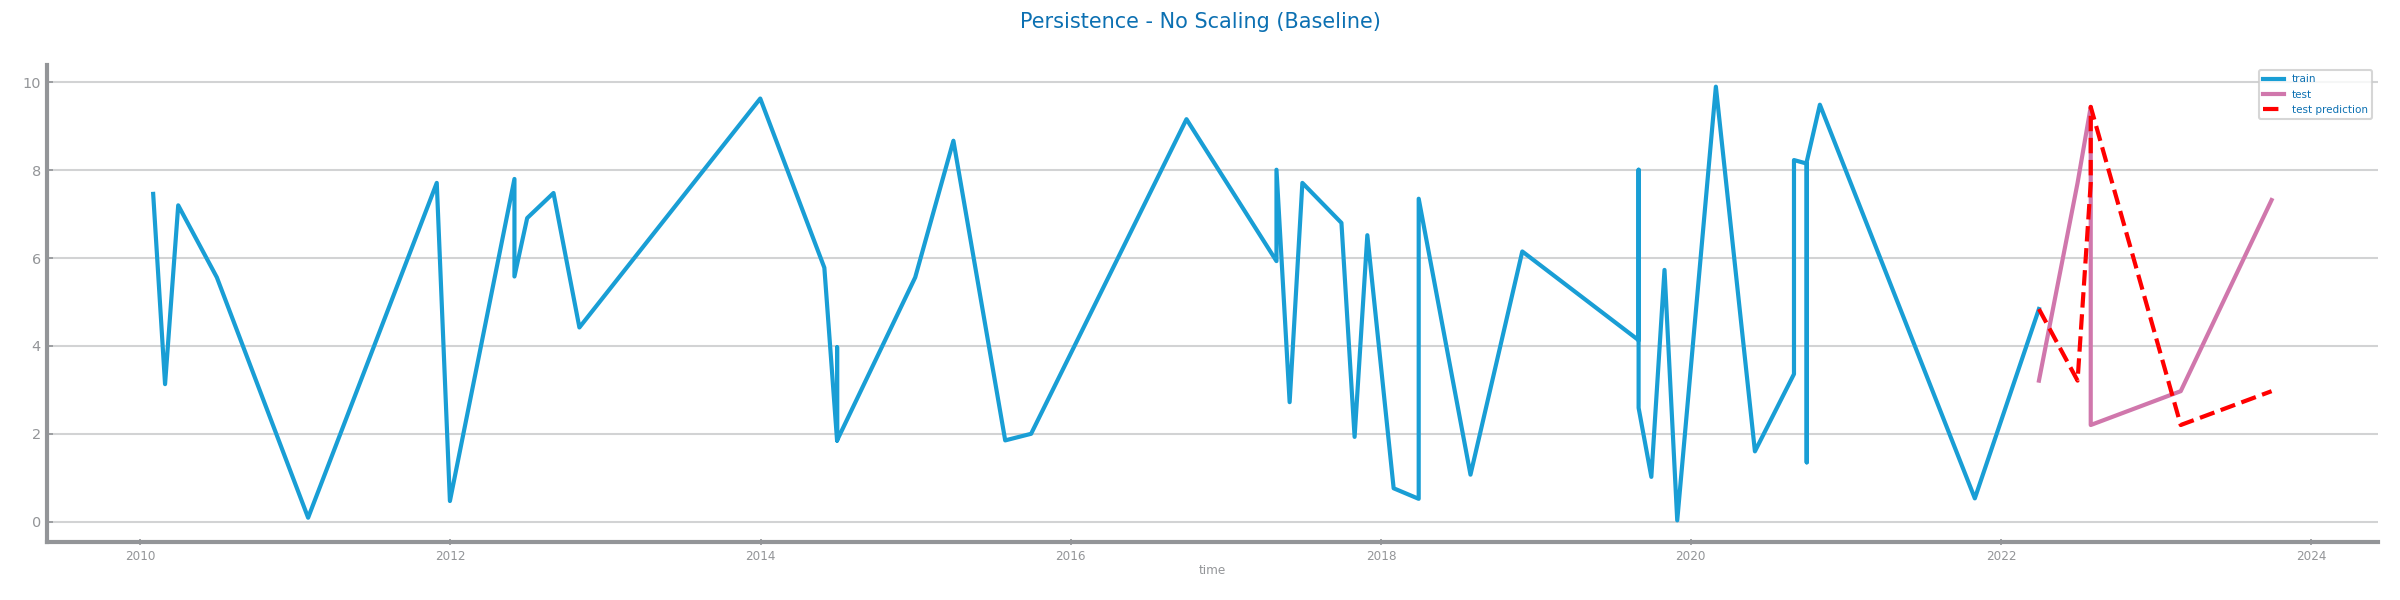
\includegraphics[width=0.9\textwidth]{economic_usa_persistence_No_Scaling_Baseline.png}
\caption{Forecasting plots obtained with Persistence model (long term) over time series 2}
\end{figure}

\begin{figure}[H]
\centering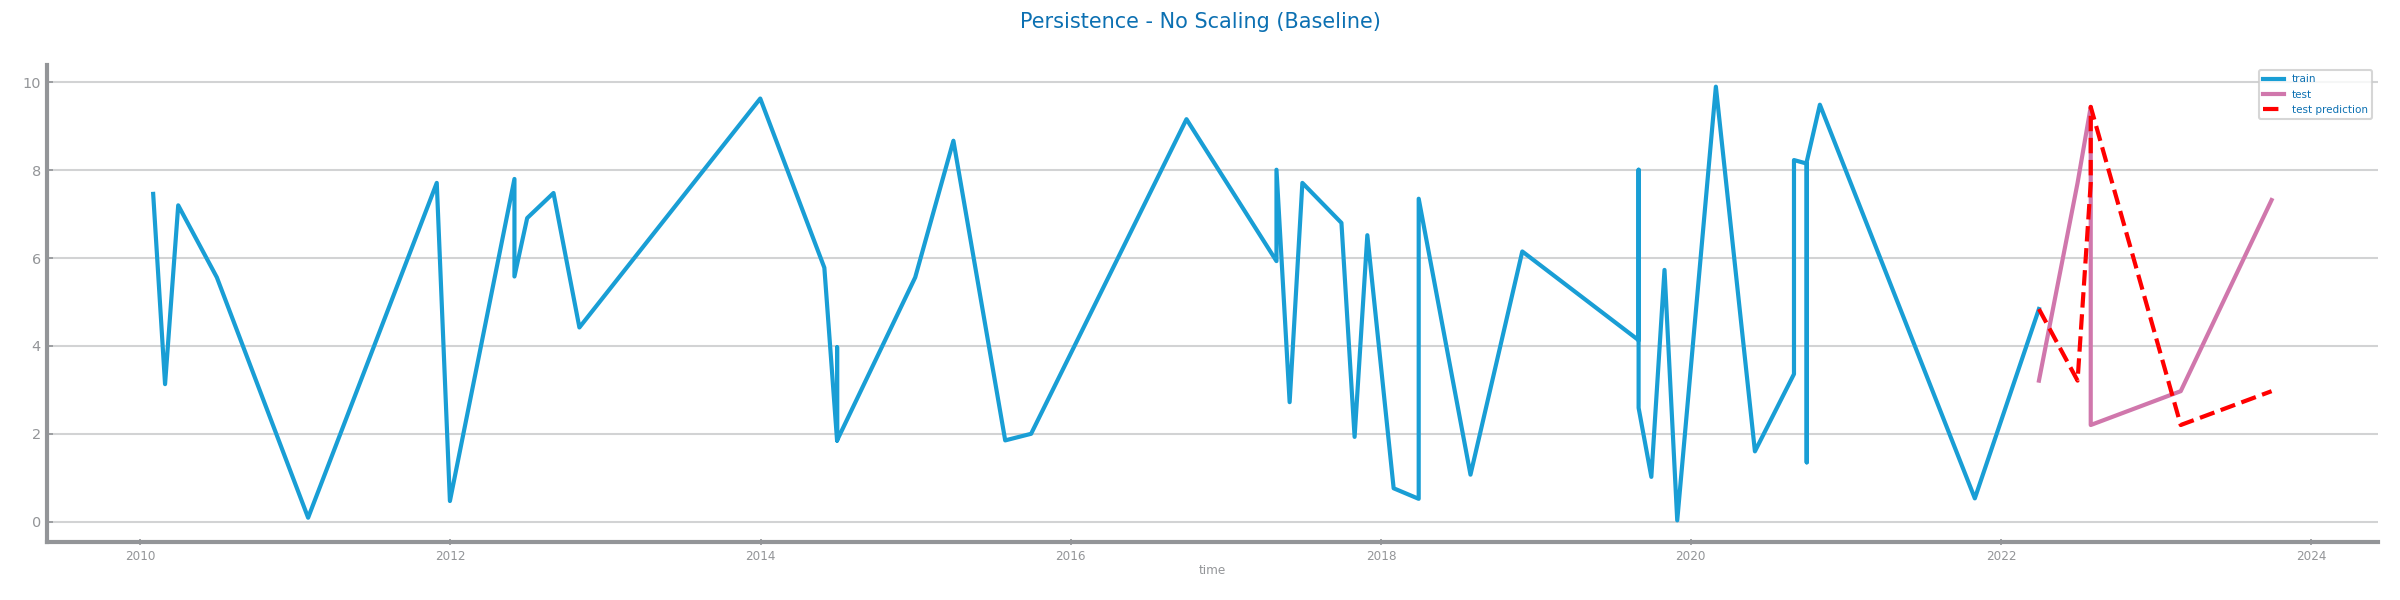
\includegraphics[width=0.9\textwidth]{economic_usa_persistence_No_Scaling_Baseline.png}
\caption{Forecasting plots obtained with Persistence model (one-set-behind) over time series 2}
\end{figure}

\begin{figure}[H]
\centering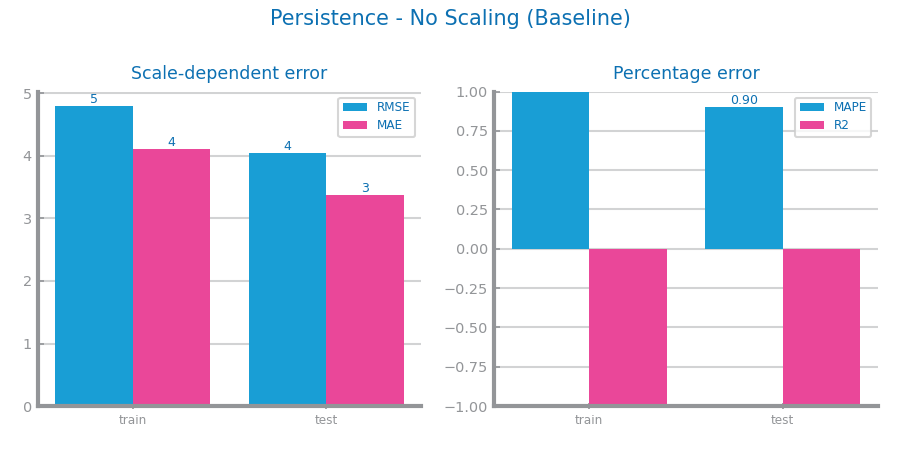
\includegraphics[width=0.9\textwidth]{economic_usa_persistence_eval_No_Scaling_Baseline.png}
\caption{Forecasting results obtained with Persistence model in both situations over time series 2}
\end{figure}

\subsection*{\textit{Rolling Mean Model}}
\ctext[RGB]{190,190,190}{Shall be used to present the results achieved through the Rolling Mean forecasting algorithms.  \textbf{Shall not exceed 500 characters.}}

\begin{figure}[H]
\centering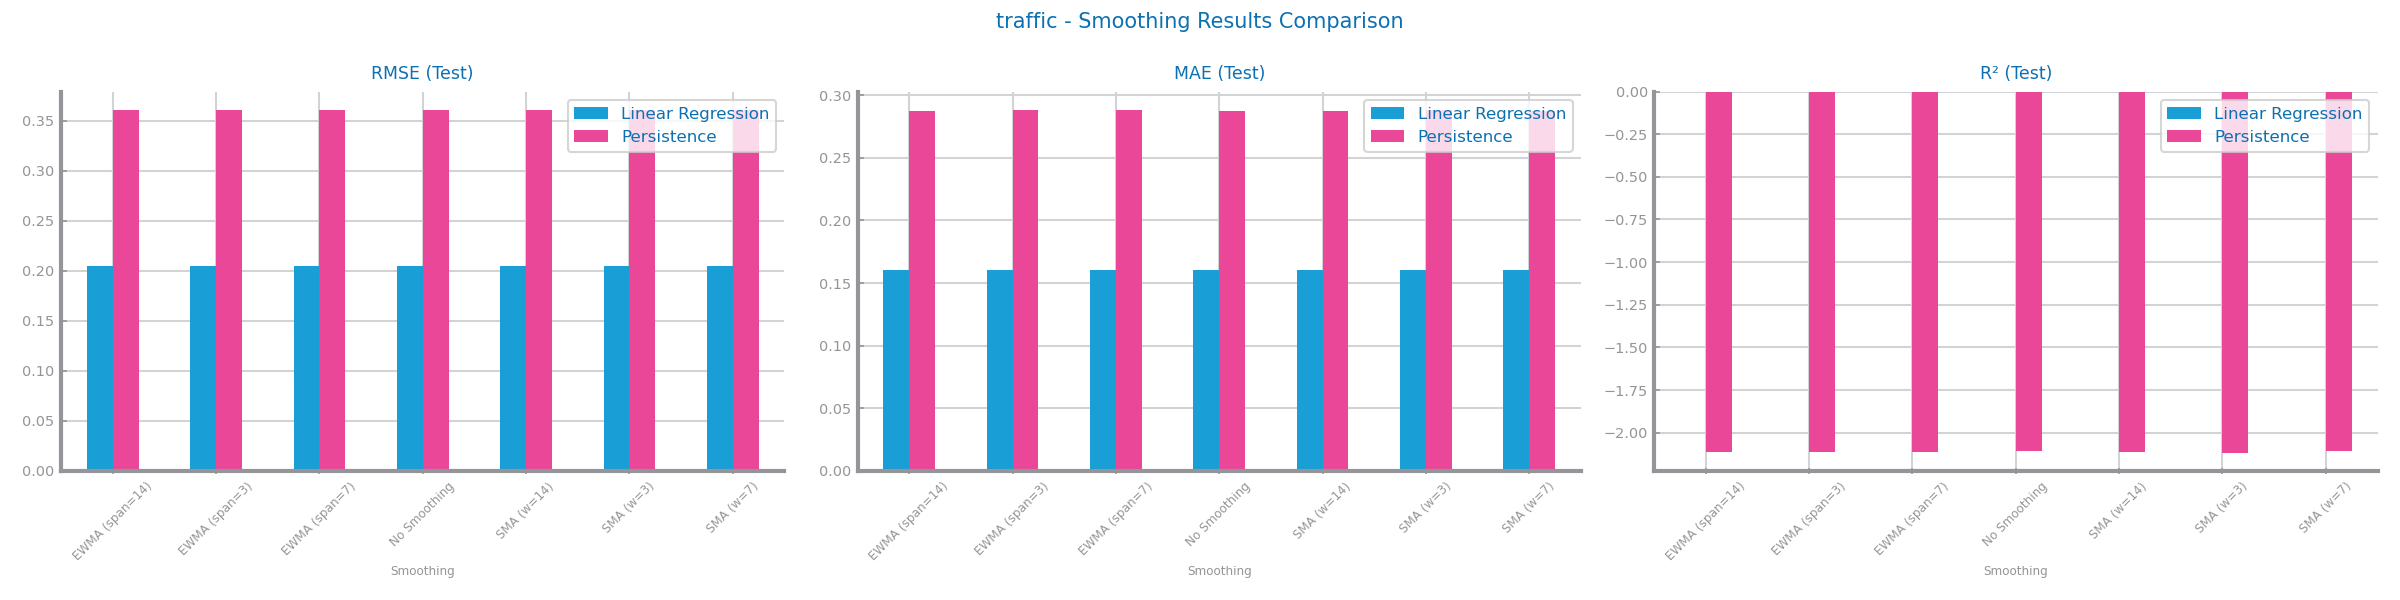
\includegraphics[width=0.9\textwidth]{traffic_smoothing_comparison_chart.png}
\caption{Forecasting study over different parameterisations of the Rolling Mean algorithm over time series 1}
\end{figure}

\begin{figure}[H]
\centering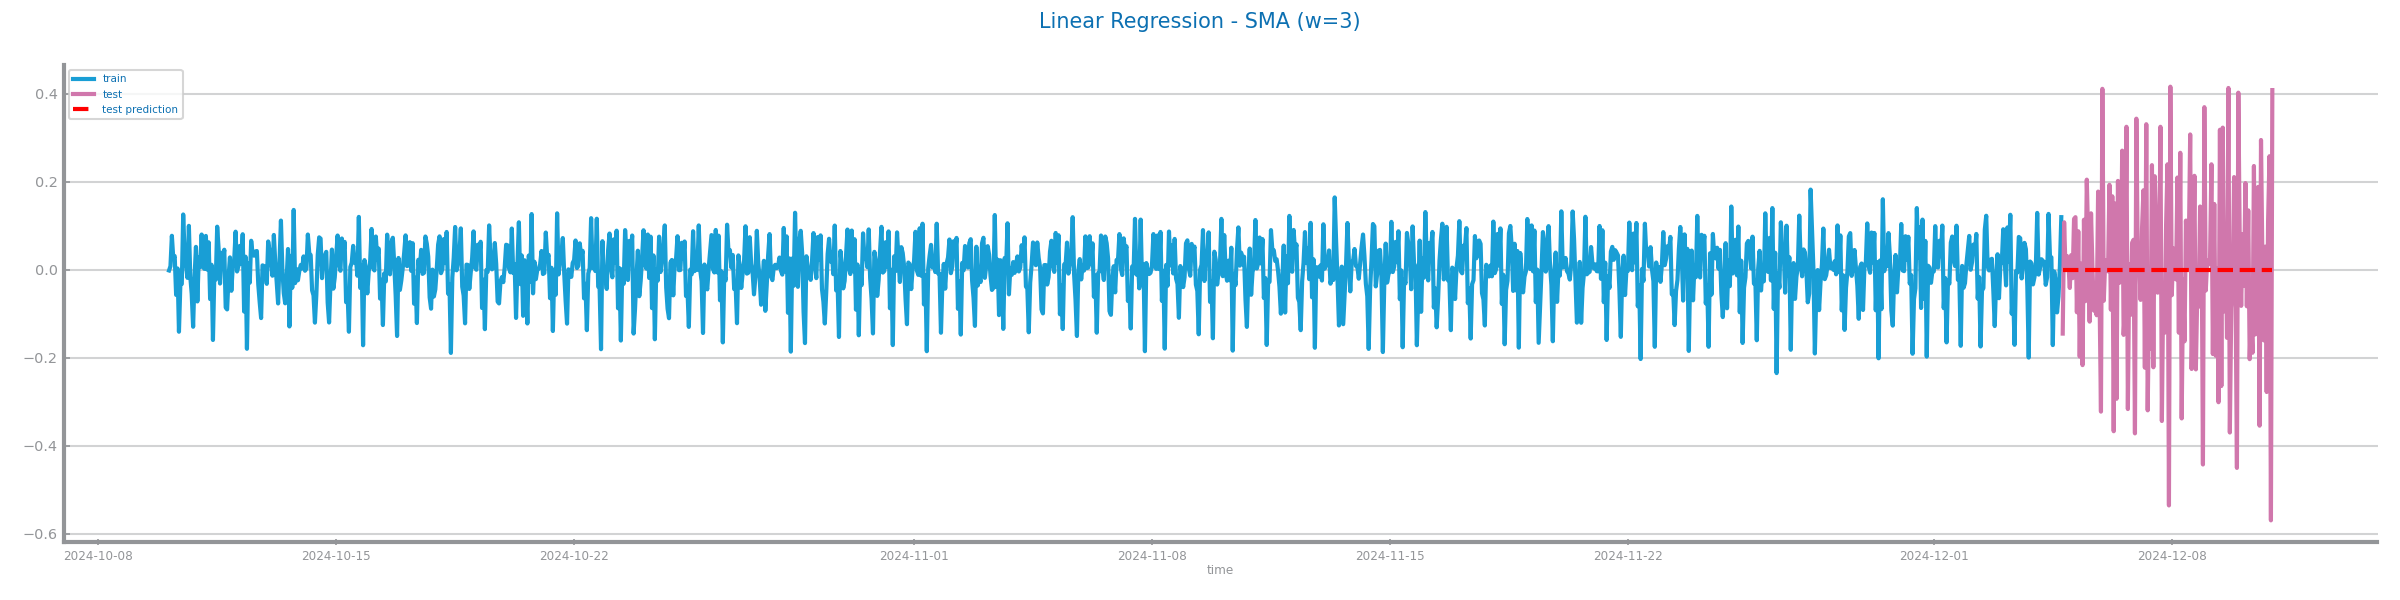
\includegraphics[width=0.9\textwidth]{traffic_lr_SMA_w3.png}
\caption{Forecasting plots obtained with the best parameterisation of Rolling Mean algorithm, over time series 1}
\end{figure}

\begin{figure}[H]
\centering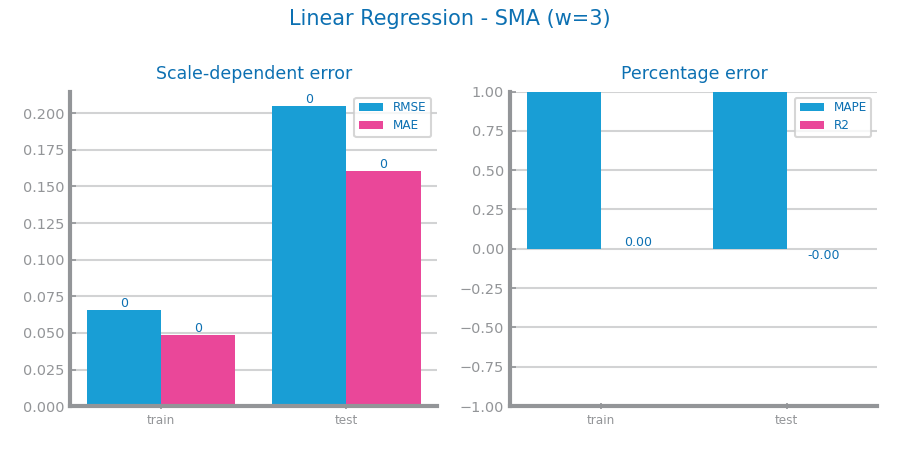
\includegraphics[width=0.9\textwidth]{traffic_lr_eval_SMA_w3.png}
\caption{Forecasting results obtained with the best parameterisation of Rolling Mean algorithm, over time series 1}
\end{figure}

\begin{figure}[H]
\centering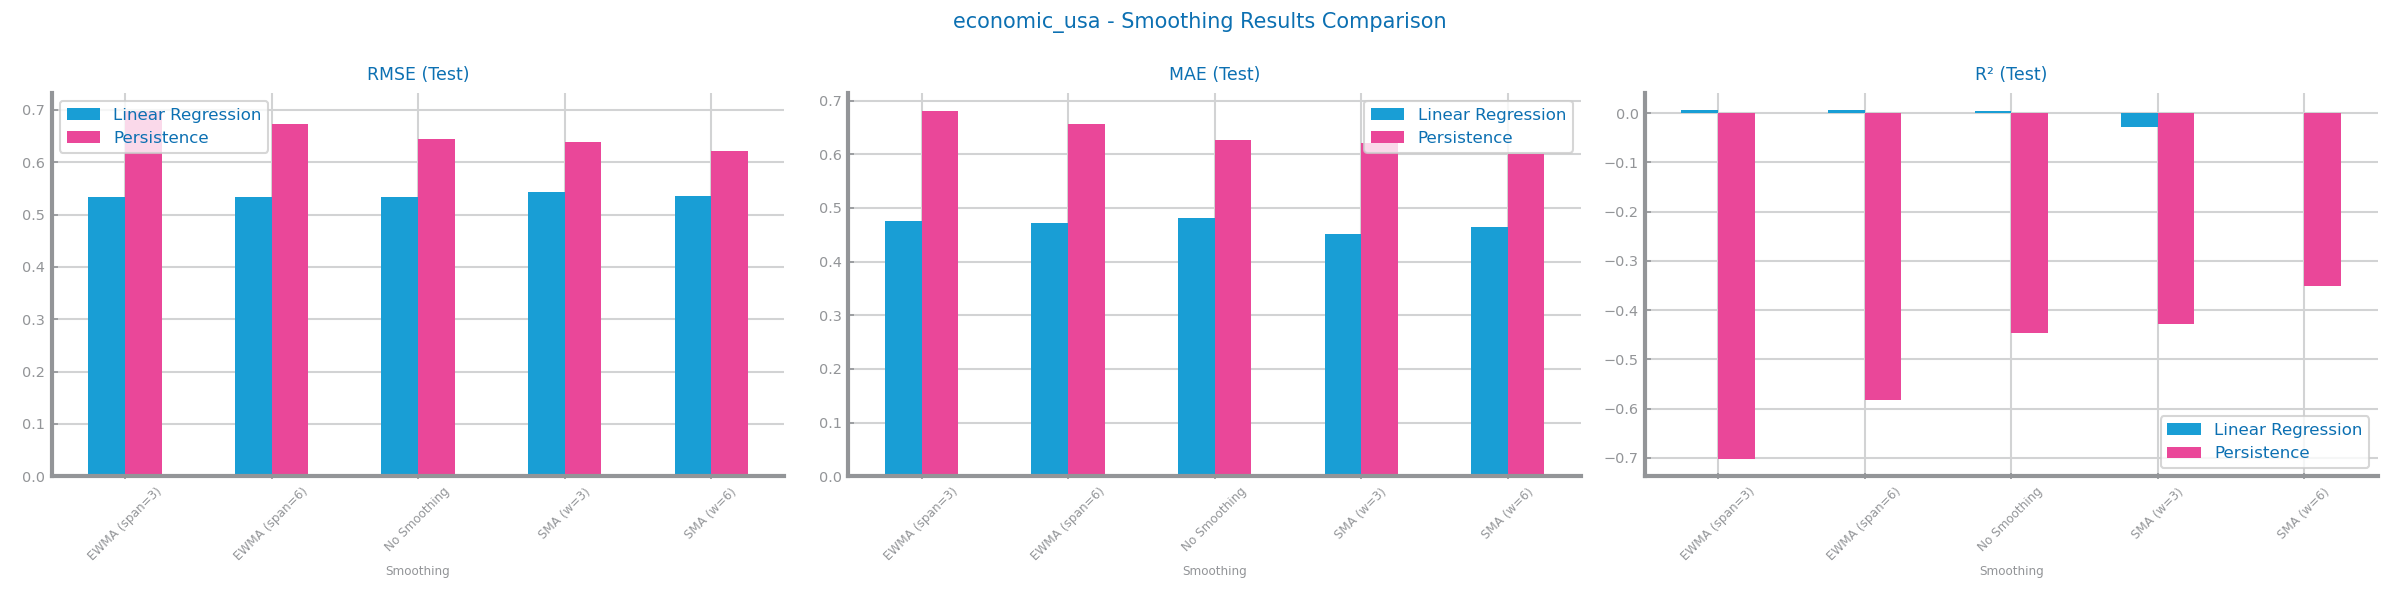
\includegraphics[width=0.9\textwidth]{economic_usa_smoothing_comparison_chart.png}
\caption{Forecasting study over different parameterisations of the Rolling Mean algorithm over time series 2}
\end{figure}

\begin{figure}[H]
\centering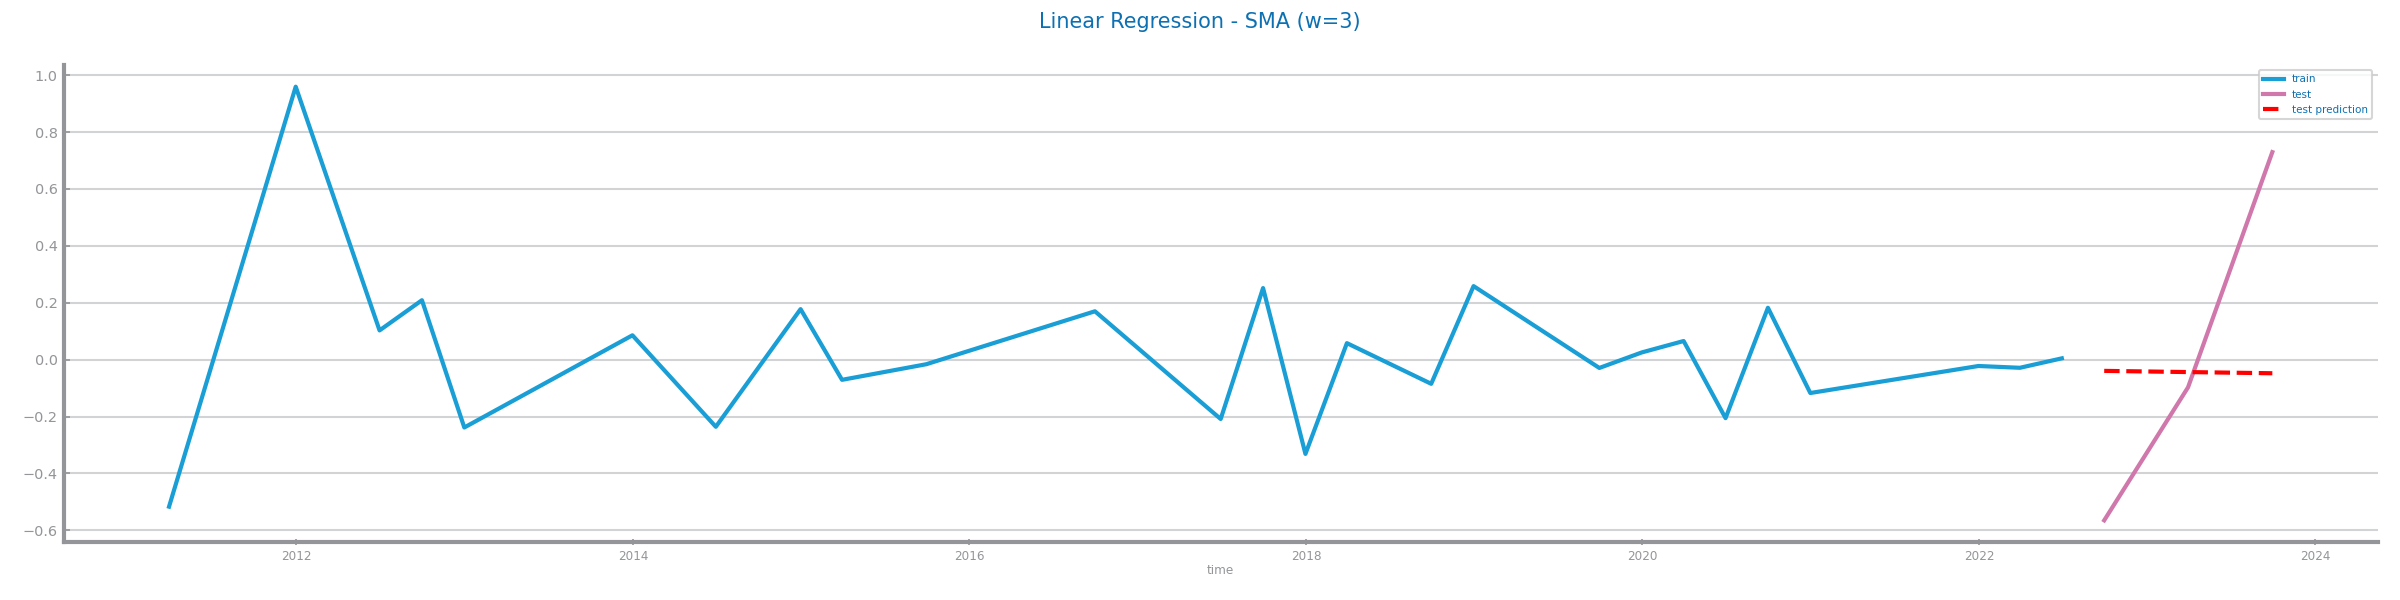
\includegraphics[width=0.9\textwidth]{economic_usa_lr_SMA_w3.png}
\caption{Forecasting plots obtained with the best parameterisation of Rolling Mean algorithm, over time series 2}
\end{figure}

\begin{figure}[H]
\centering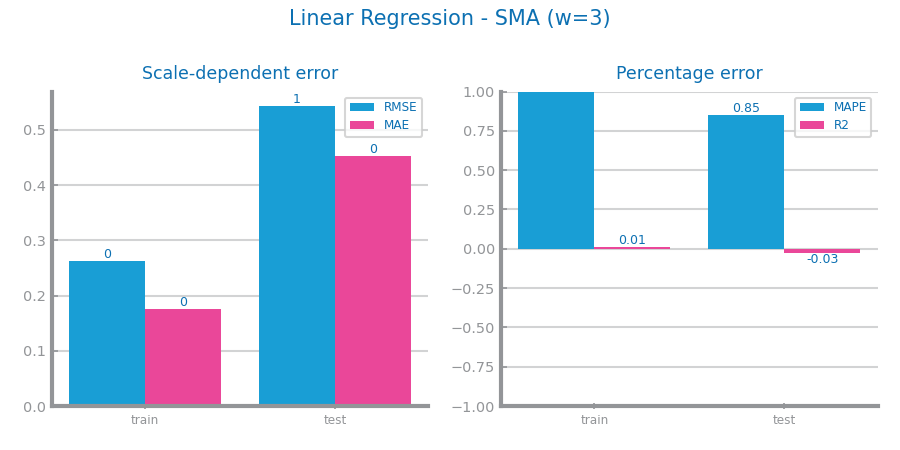
\includegraphics[width=0.9\textwidth]{economic_usa_lr_eval_SMA_w3.png}
\caption{Forecasting results obtained with the best parameterisation of Rolling Mean algorithm, over time series 2}
\end{figure}

\subsection*{\textit{Exponential Smoothing Model}}
\ctext[RGB]{190,190,190}{Shall be used to present the results achieved through the Exponential Smoothing forecasting algorithms.  \textbf{Shall not exceed 500 characters.}}

\begin{figure}[H]
\centering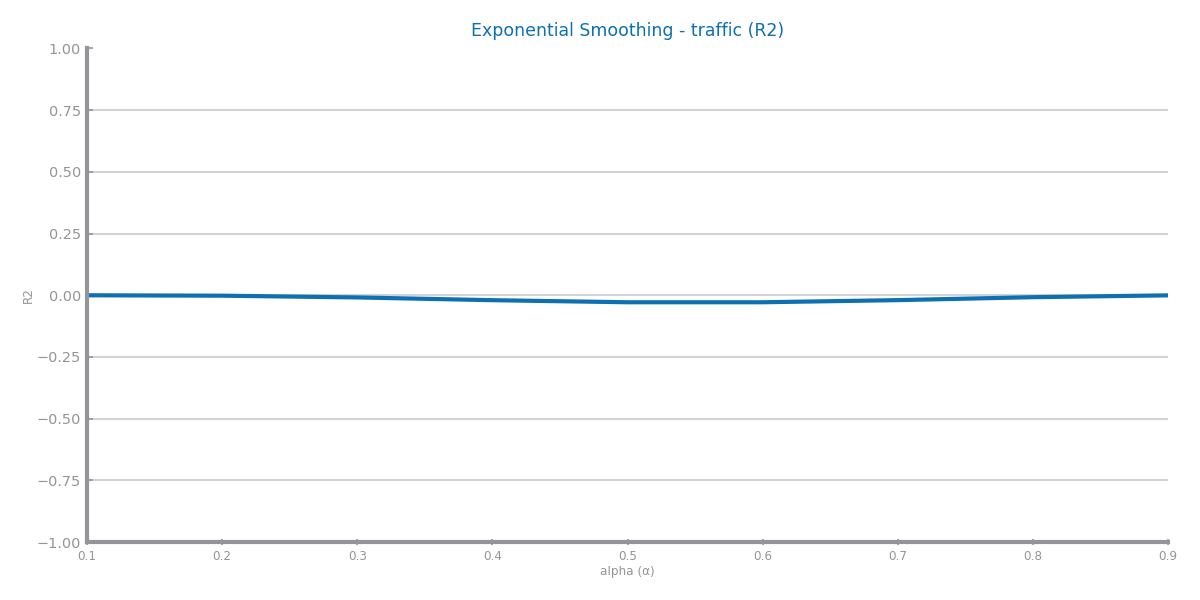
\includegraphics[width=0.9\textwidth]{traffic_exponential_smoothing_R2_study.png}
\caption{Forecasting study over different parameterisations of the Exponential Smoothing algorithm over time series 1}
\end{figure}

\begin{figure}[H]
\centering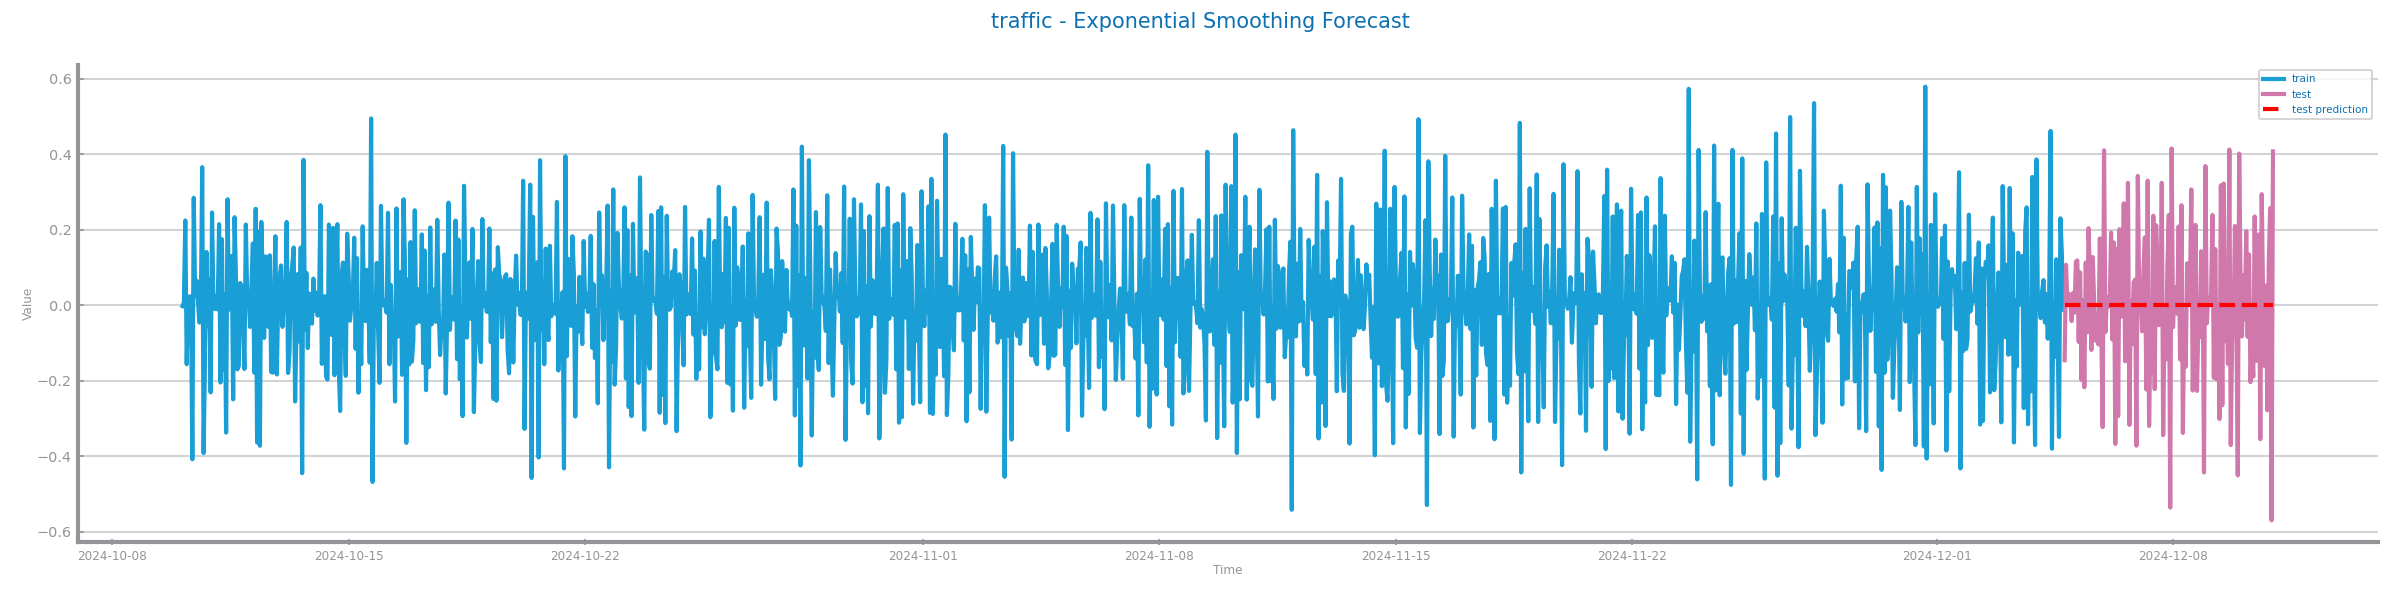
\includegraphics[width=0.9\textwidth]{traffic_exponential_smoothing_forecast.png}
\caption{Forecasting plots obtained with the best parameterisation of Exponential Smoothing algorithm, over time series 1}
\end{figure}

\begin{figure}[H]
\centering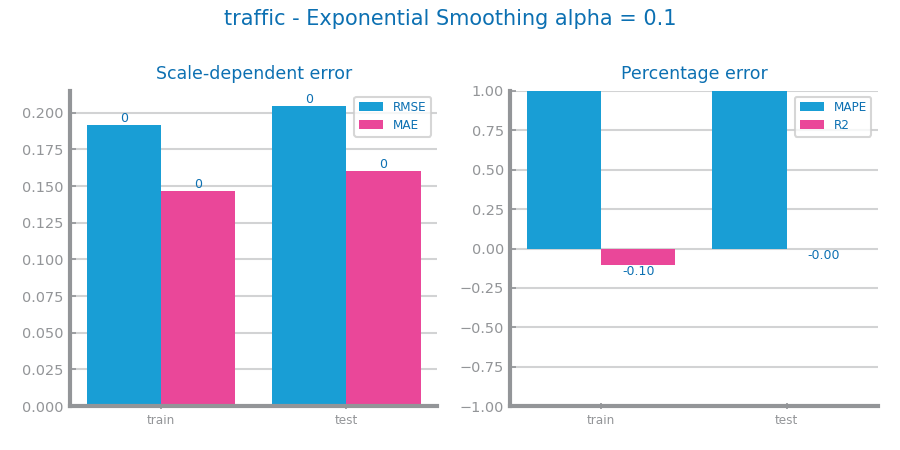
\includegraphics[width=0.9\textwidth]{traffic_exponential_smoothing_eval.png}
\caption{Forecasting results obtained with the best parameterisation of Exponential Smoothing algorithm, over time series 1}
\end{figure}

\begin{figure}[H]
\centering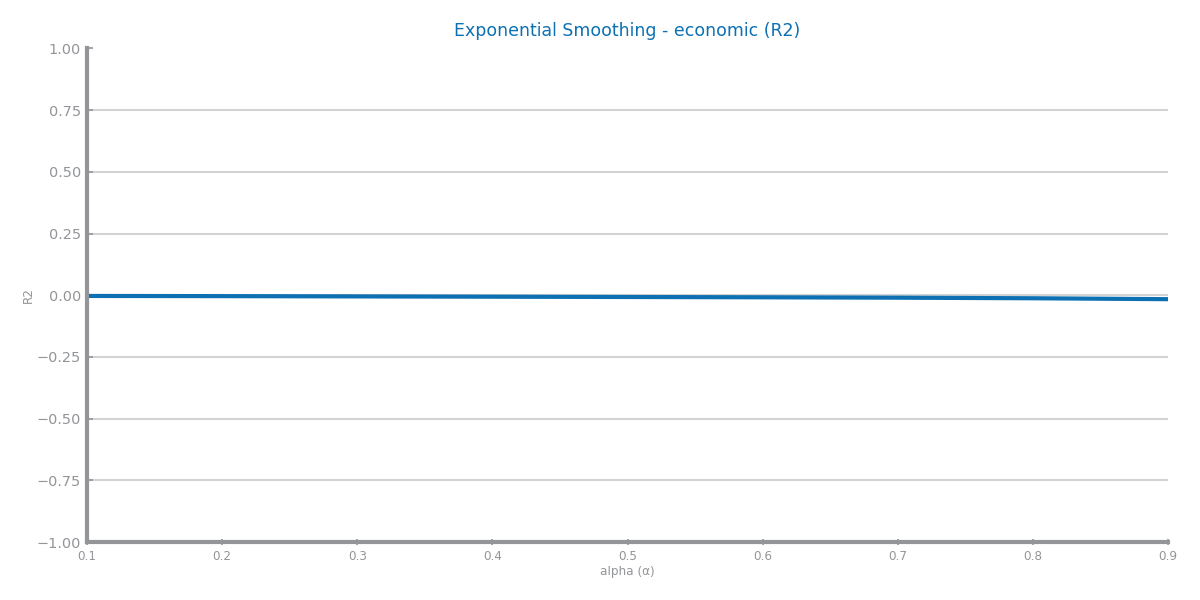
\includegraphics[width=0.9\textwidth]{economic_exponential_smoothing_R2_study.png}
\caption{Forecasting study over different parameterisations of the Exponential Smoothing algorithm over time series 2}
\end{figure}

\begin{figure}[H]
\centering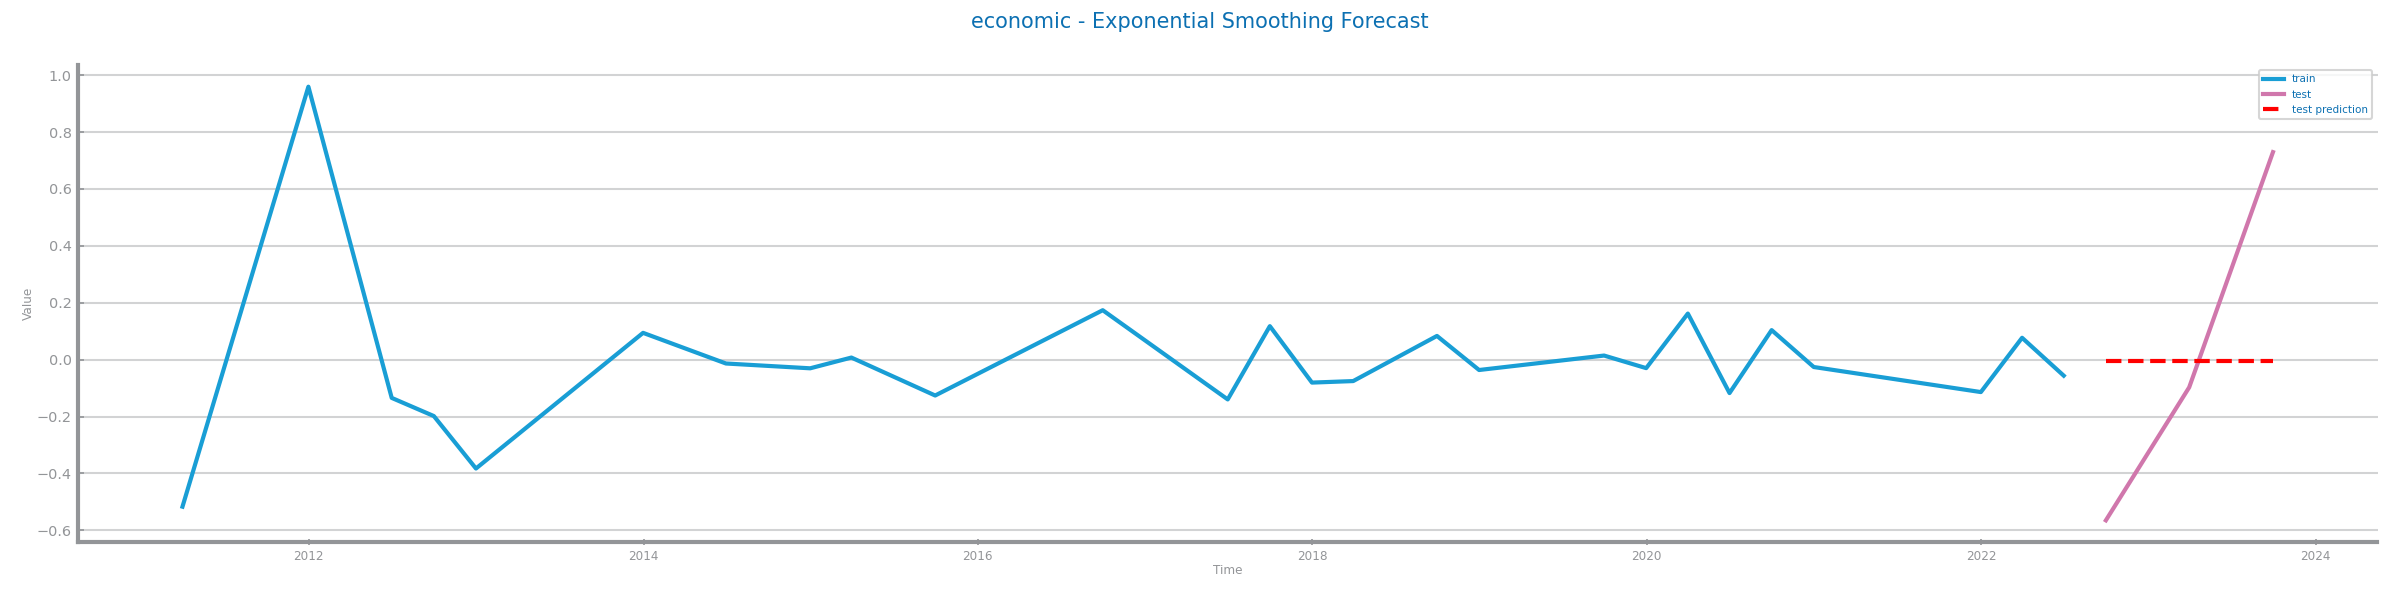
\includegraphics[width=0.9\textwidth]{economic_exponential_smoothing_forecast.png}
\caption{Forecasting plots obtained with the best parameterisation of Exponential Smoothing algorithm, over time series 2}
\end{figure}

\begin{figure}[H]
\centering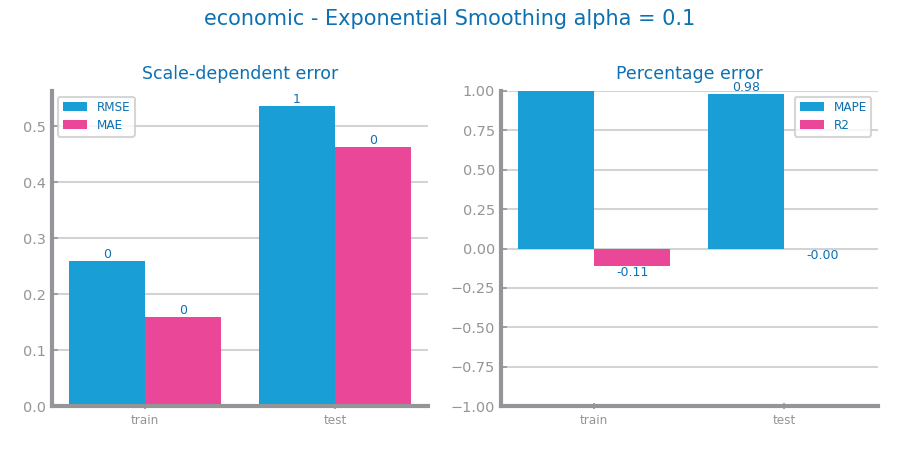
\includegraphics[width=0.9\textwidth]{economic_exponential_smoothing_eval.png}
\caption{Forecasting results obtained with the best parameterisation of Exponential Smoothing algorithm, over time series 2}
\end{figure}

\subsection*{\textit{Linear Regression Model}}
\ctext[RGB]{190,190,190}{Shall be used to present the results achieved through the simple average model.  \textbf{Shall not exceed 200 characters.}}

\begin{figure}[H]
\centering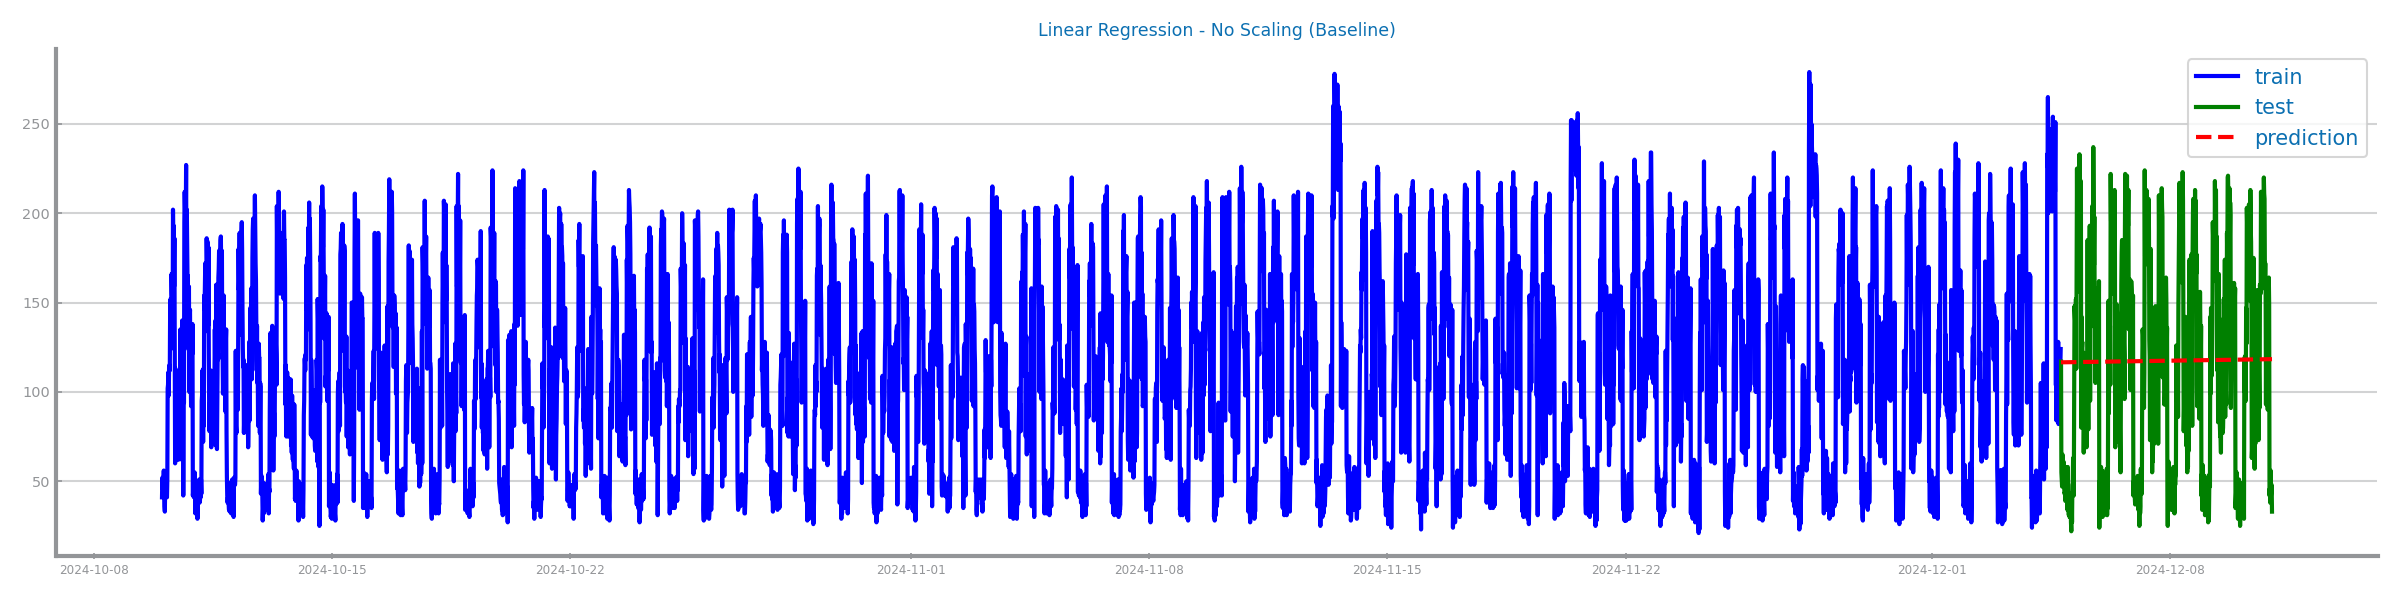
\includegraphics[width=0.9\textwidth]{traffic_lr_none.png}
\caption{Forecasting plots obtained with Linear Regression model over time series 1}
\end{figure}

\begin{figure}[H]
\centering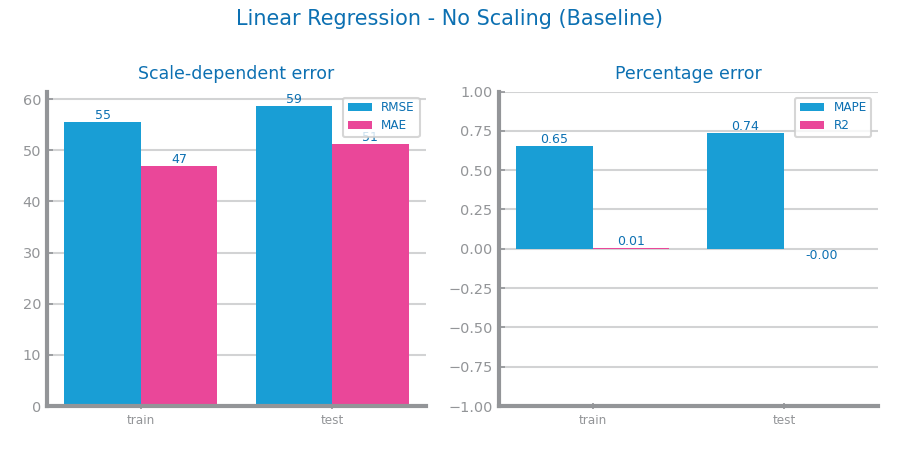
\includegraphics[width=0.9\textwidth]{traffic_lr_eval_none.png}
\caption{Forecasting results obtained with Linear Regression model over time series 1}
\end{figure}

\begin{figure}[H]
\centering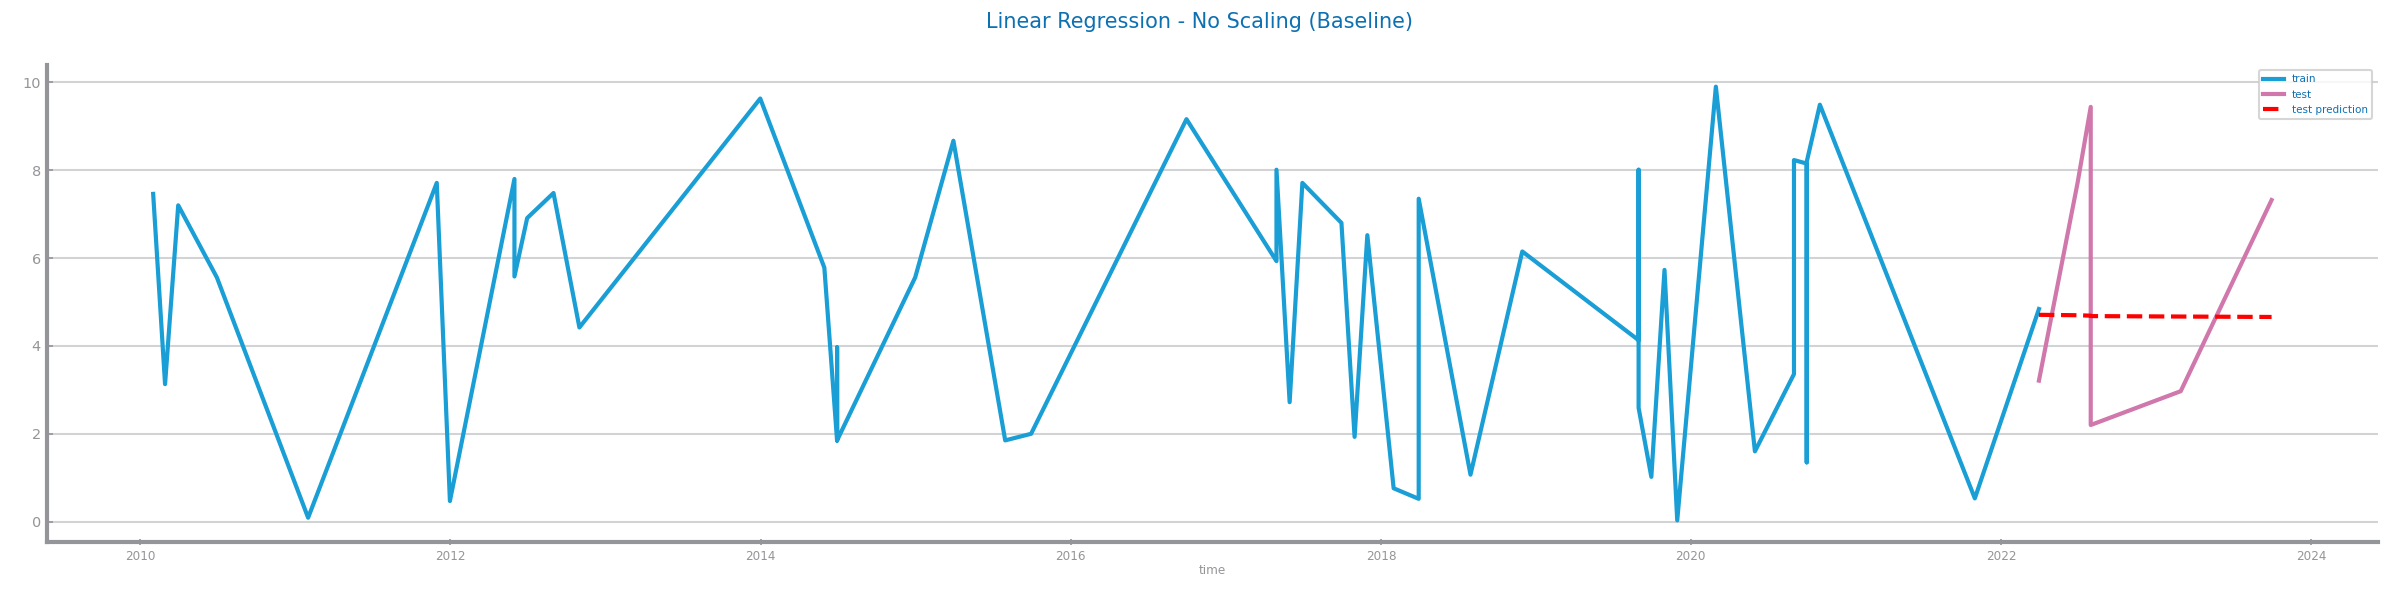
\includegraphics[width=0.9\textwidth]{economic_usa_lr_No_Scaling_Baseline.png}
\caption{Forecasting plots obtained with Linear Regression model over time series 2}
\end{figure}

\begin{figure}[H]
\centering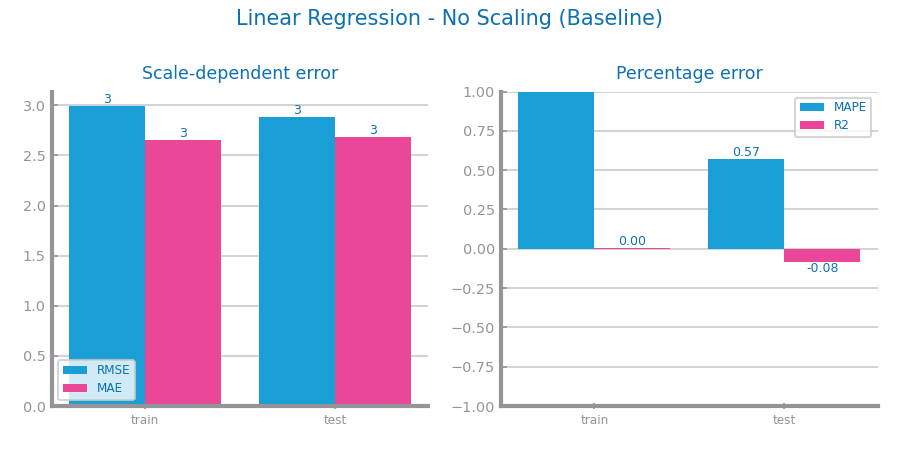
\includegraphics[width=0.9\textwidth]{economic_usa_lr_eval_No_Scaling_Baseline.png}
\caption{Forecasting results obtained with Linear Regression model over time series 2}
\end{figure}

\subsection*{\textit{ARIMA Model}}
\ctext[RGB]{190,190,190}{Shall be used to present the results achieved through the ARIMA forecasting algorithms.  \textbf{Shall not exceed 500 characters.}}

\begin{figure}[H]
\centering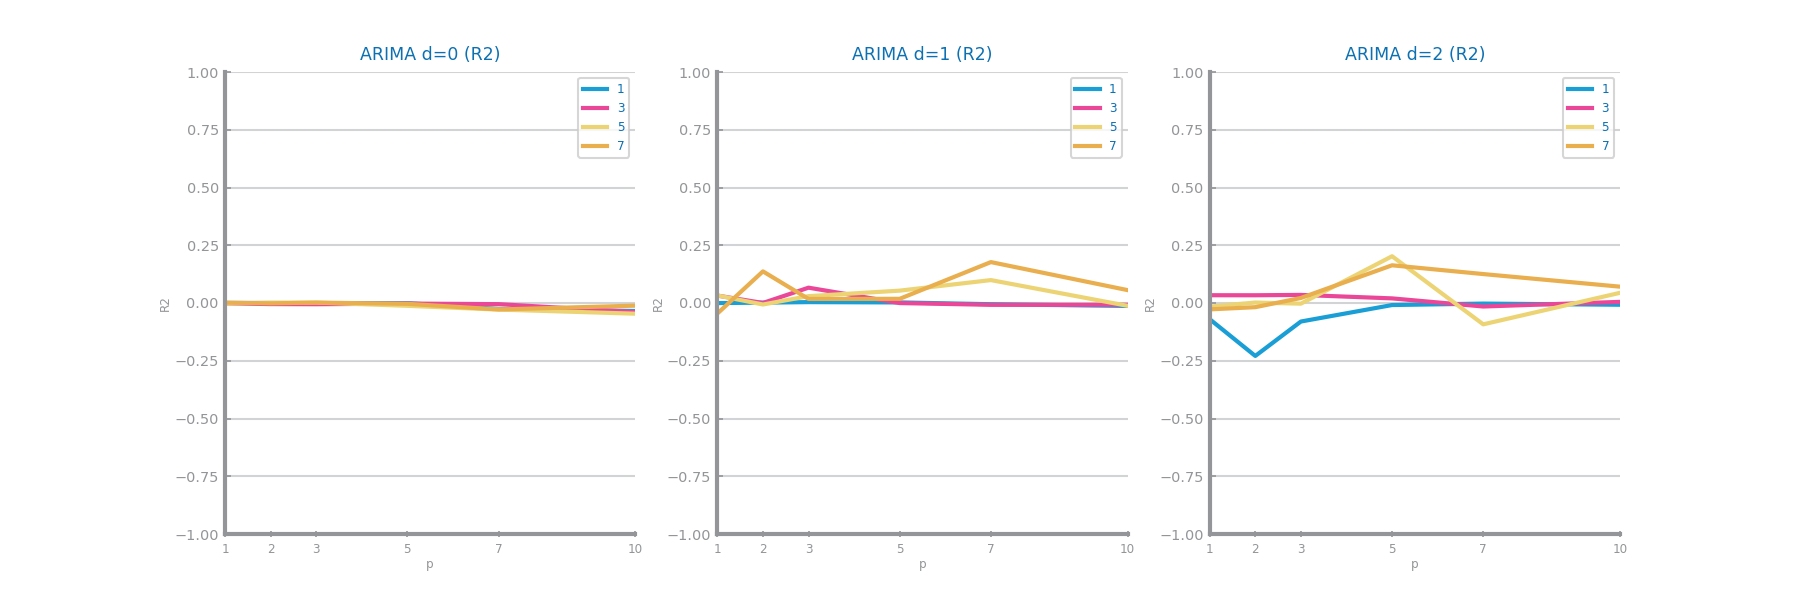
\includegraphics[width=0.9\textwidth]{traffic_arima_R2_study.png}
\caption{Forecasting study over different parameterisations of the ARIMA algorithm over time series 1, only with the target variable}
\end{figure}

\begin{figure}[H]
\centering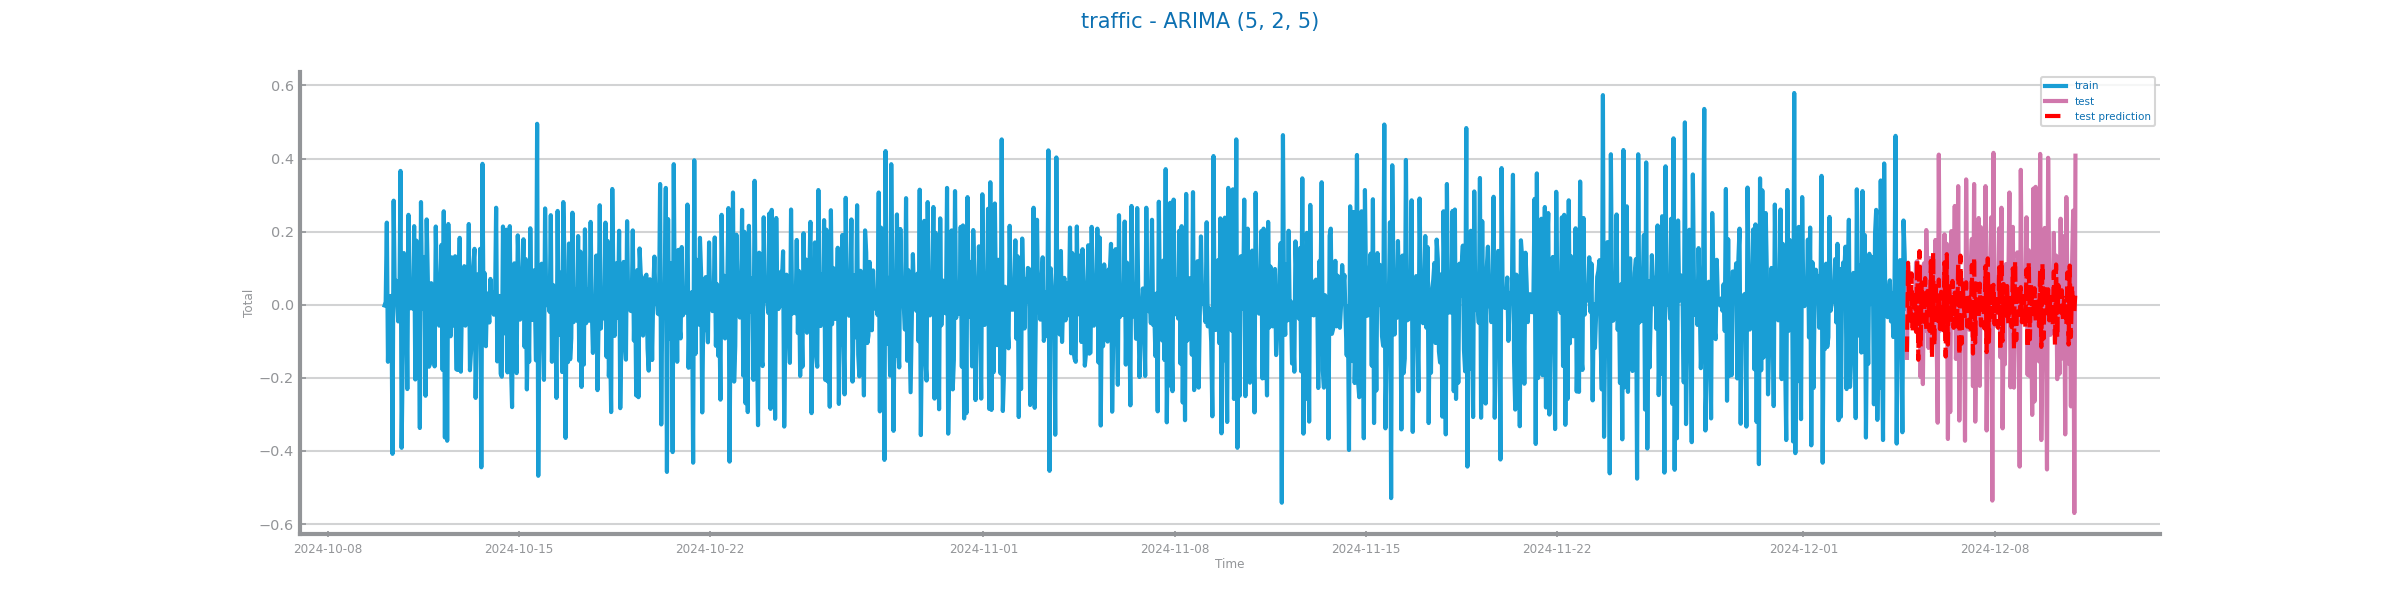
\includegraphics[width=0.9\textwidth]{traffic_arima_R2_forecast.png}
\caption{Forecasting plots obtained with the best parameterisation of ARIMA algorithm, over time series 1, only with the target variable}
\end{figure}

\begin{figure}[H]
\centering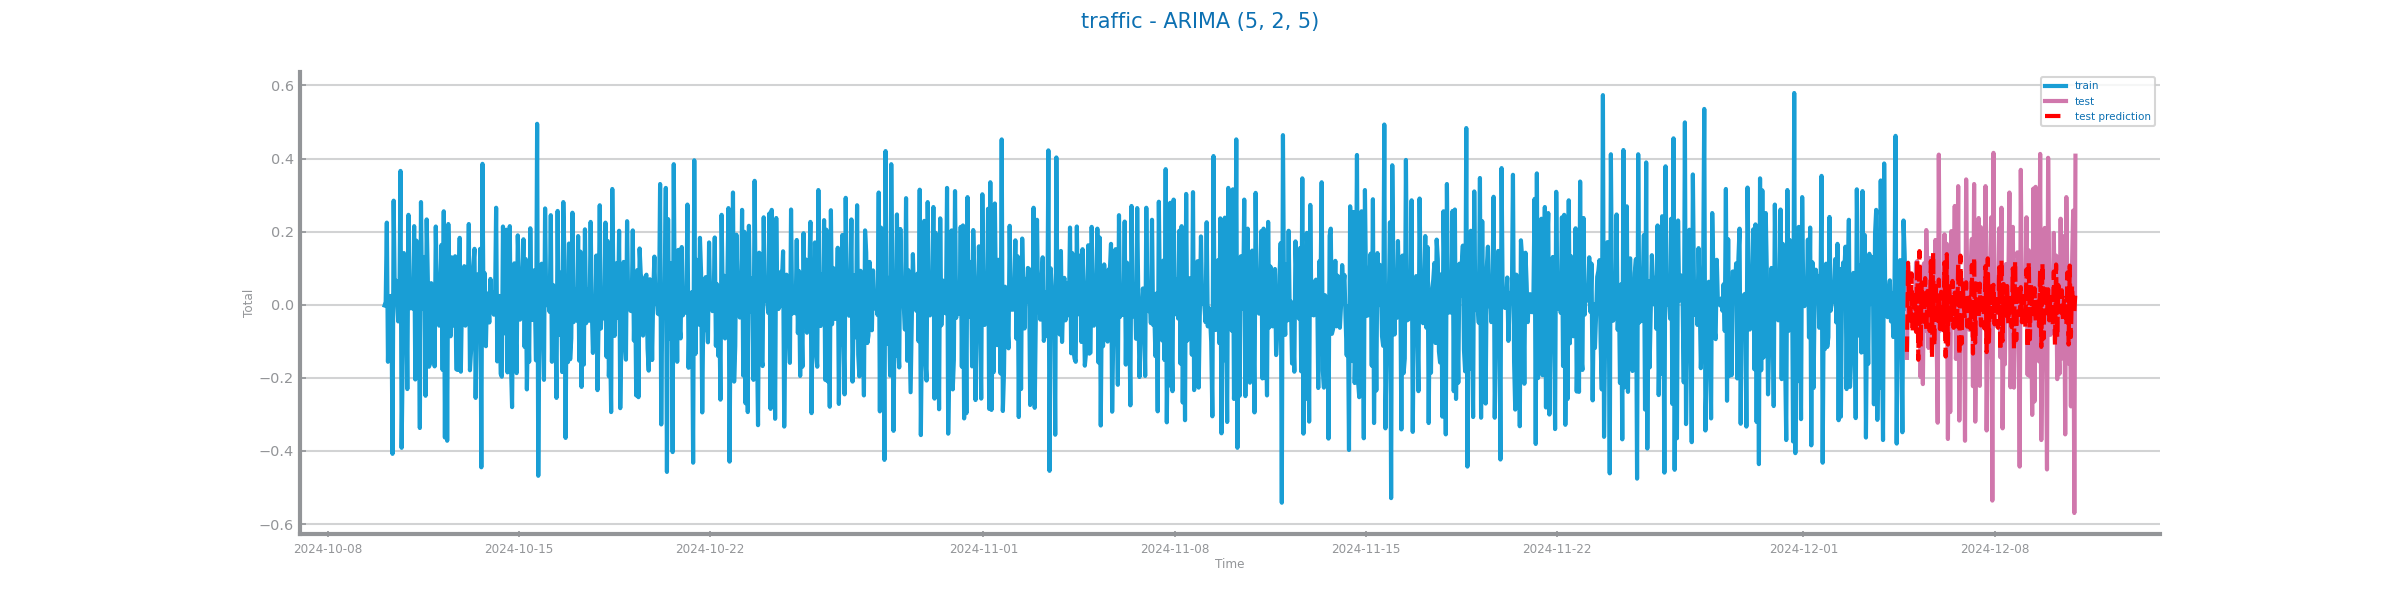
\includegraphics[width=0.9\textwidth]{traffic_arima_R2_forecast.png}
\caption{Forecasting results obtained with the best parameterisation of ARIMA algorithm, over time series 1, only with the target variable}
\end{figure}

\begin{figure}[H]
\centering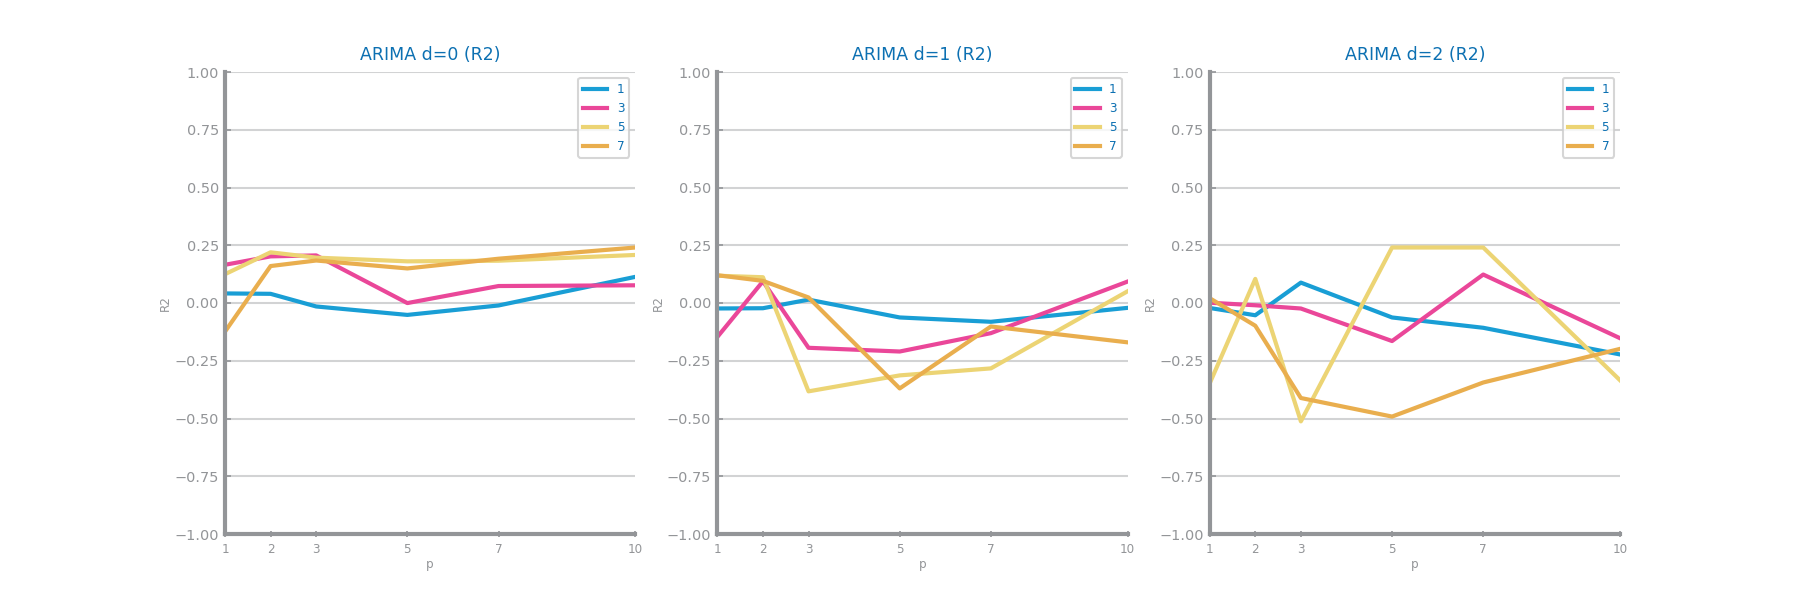
\includegraphics[width=0.9\textwidth]{economic_arima_R2_study.png}
\caption{Forecasting study over different parameterisations of the ARIMA algorithm over time series 2, only with the target variable}
\end{figure}

\begin{figure}[H]
\centering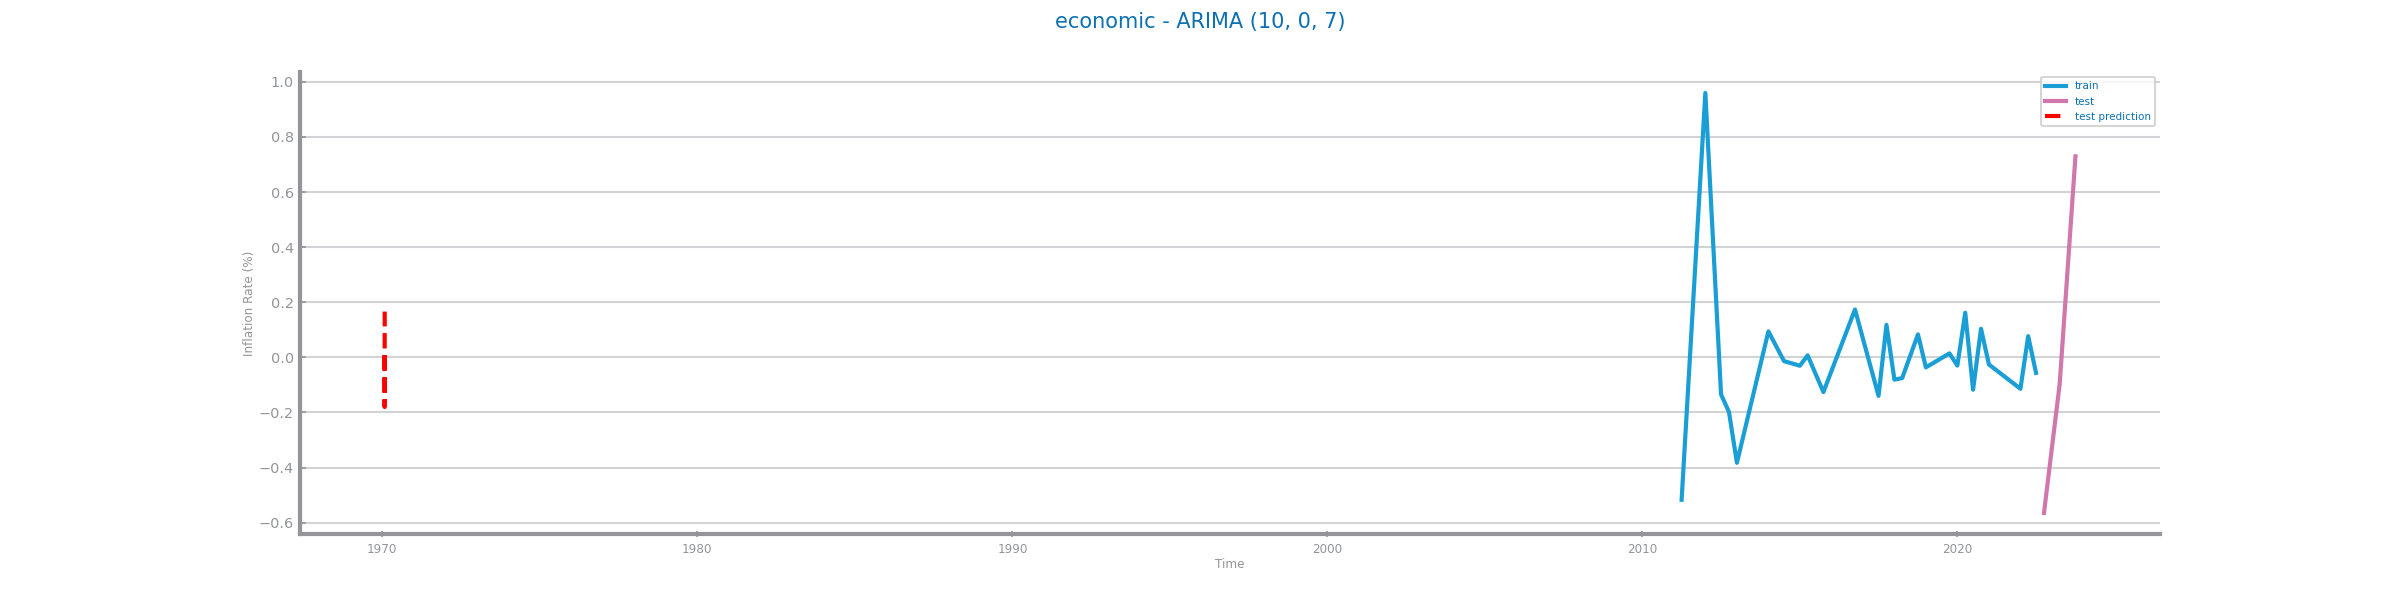
\includegraphics[width=0.9\textwidth]{economic_arima_R2_forecast.png}
\caption{Forecasting plots obtained with the best parameterisation of ARIMA algorithm, over time series 2, only with the target variable}
\end{figure}

\begin{figure}[H]
\centering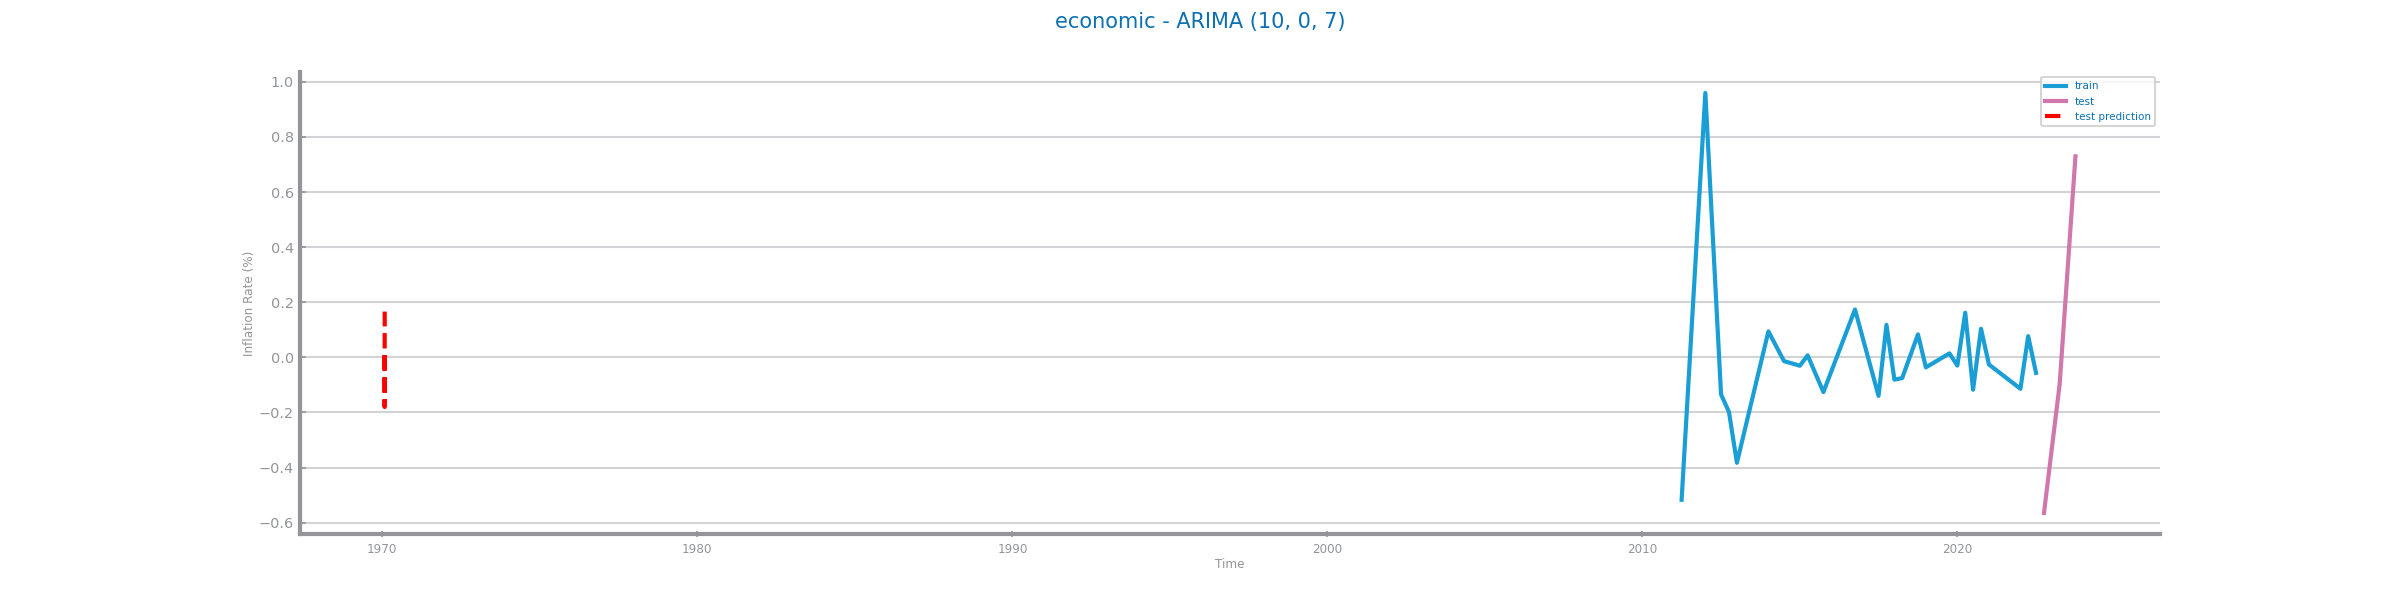
\includegraphics[width=0.9\textwidth]{economic_arima_R2_forecast.png}
\caption{Forecasting results obtained with the best parameterisation of ARIMA algorithm, over time series 2, only with the target variable}
\end{figure}

\begin{figure}[H]
\centering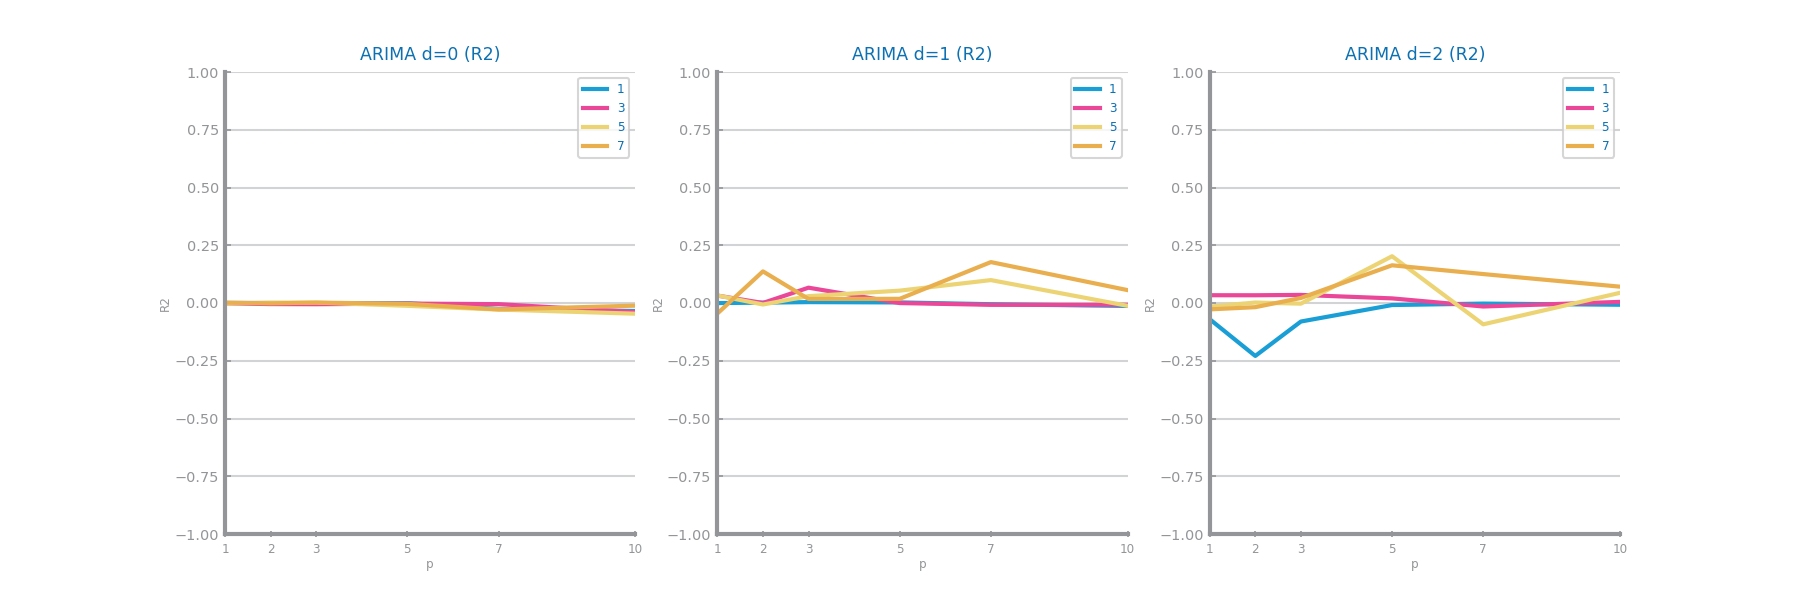
\includegraphics[width=0.9\textwidth]{traffic_arima_R2_study.png}
\caption{Forecasting study over different parameterisations of the ARIMA algorithm with multiple variables over time series 1}
\end{figure}

\begin{figure}[H]
\centering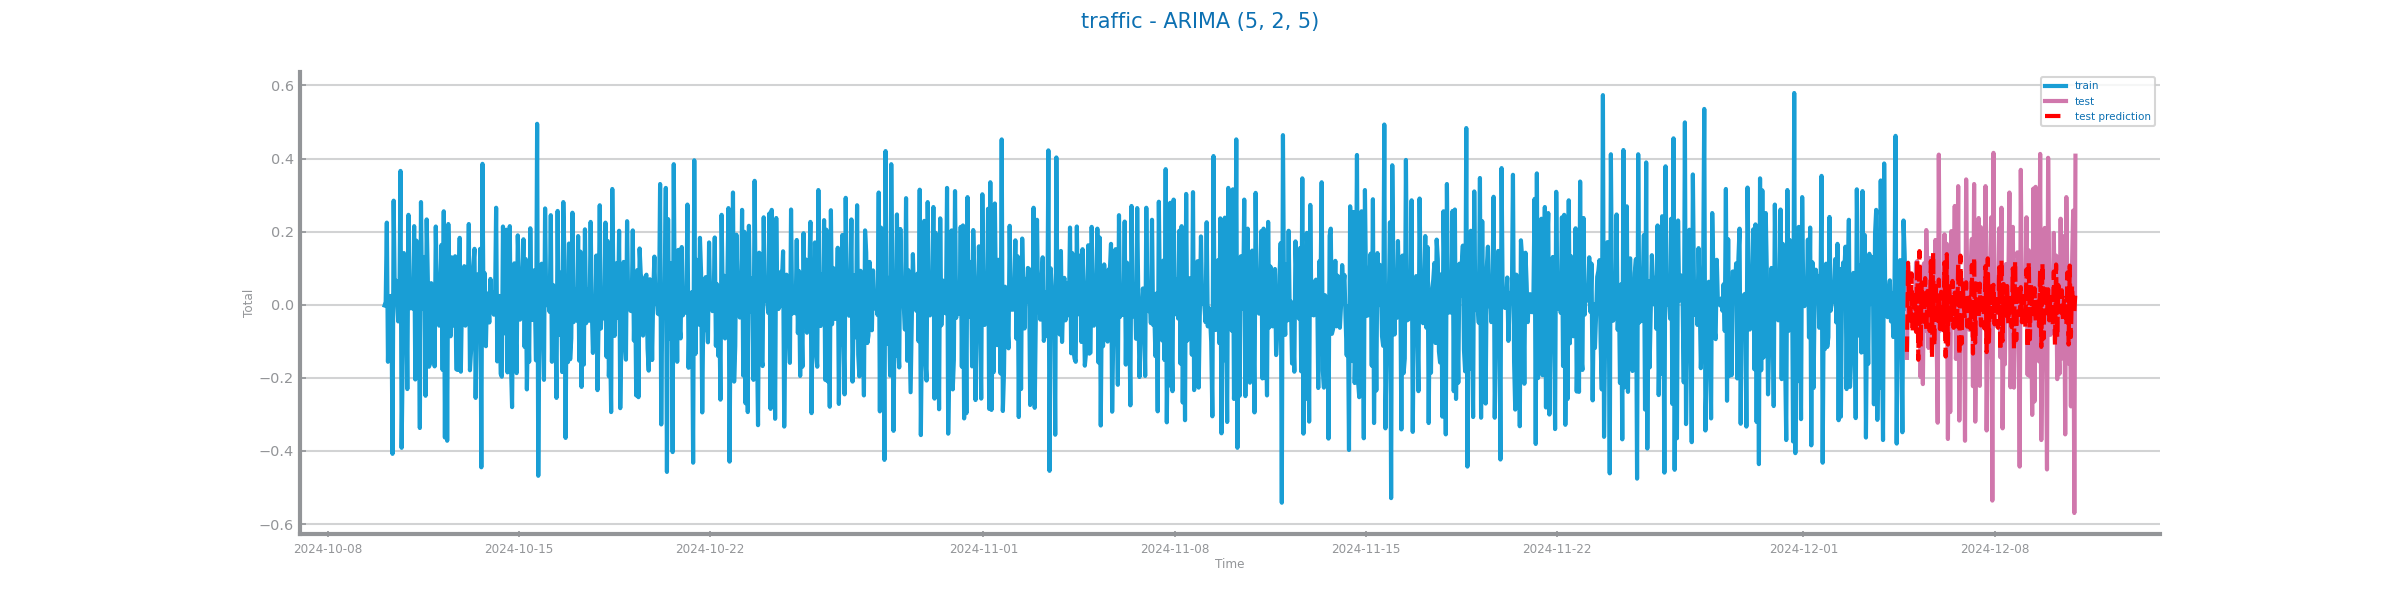
\includegraphics[width=0.9\textwidth]{traffic_arima_R2_forecast.png}
\caption{Forecasting plots obtained with the best parameterisation of ARIMA algorithm with multiple variables over time series 1}
\end{figure}

\begin{figure}[H]
\centering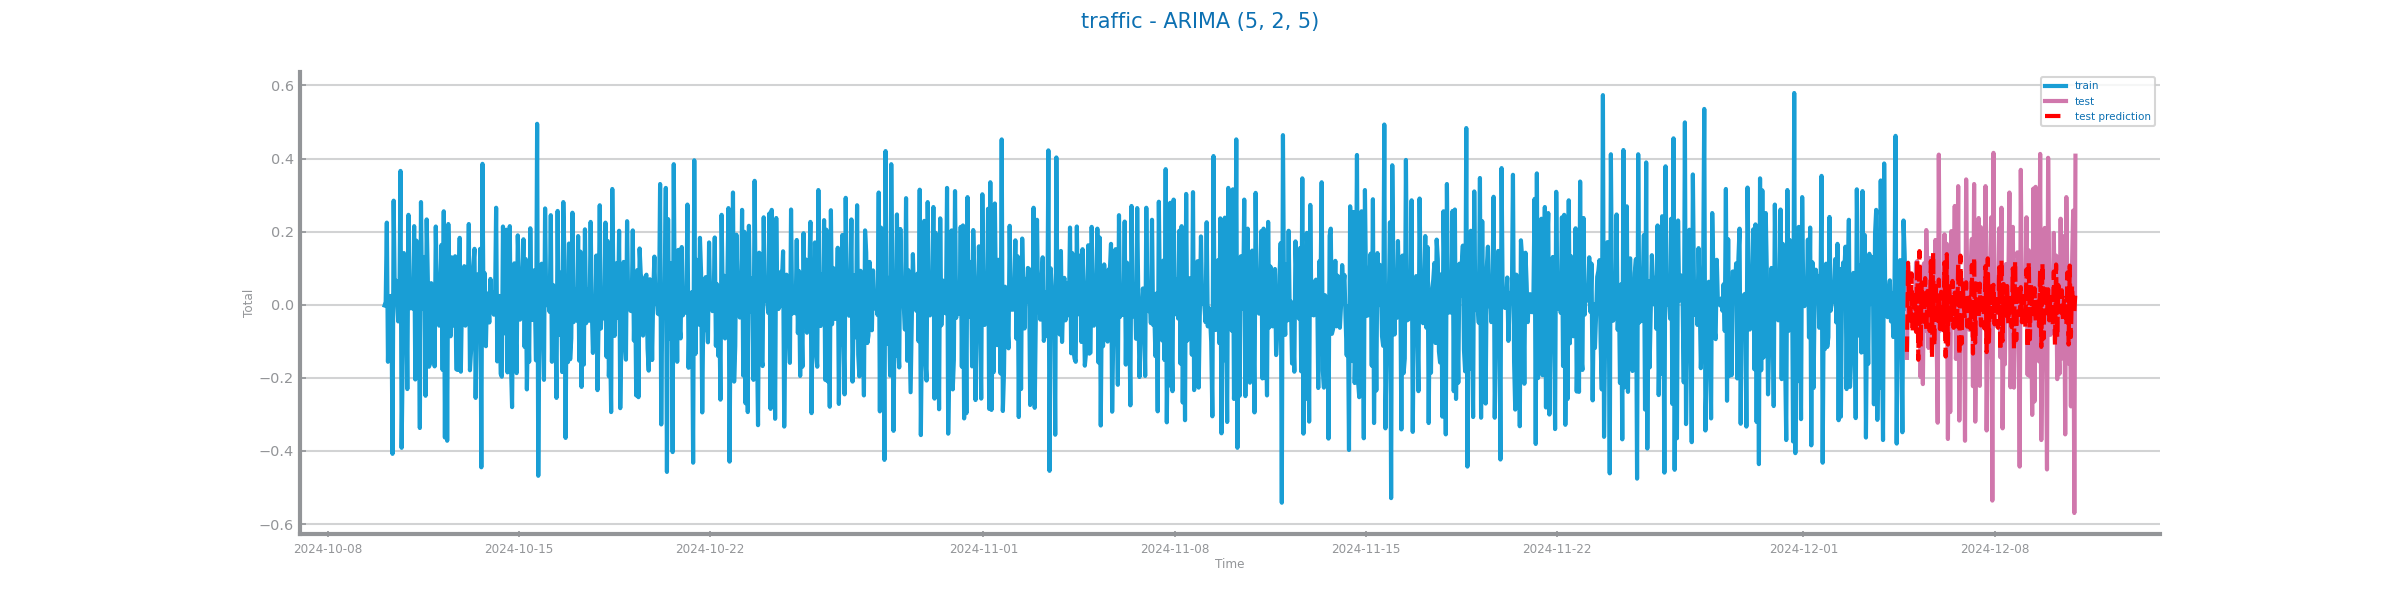
\includegraphics[width=0.9\textwidth]{traffic_arima_R2_forecast.png}
\caption{Forecasting results obtained with the best parameterisation of ARIMA algorithm with multiple variables over time series 1}
\end{figure}

\begin{figure}[H]
\centering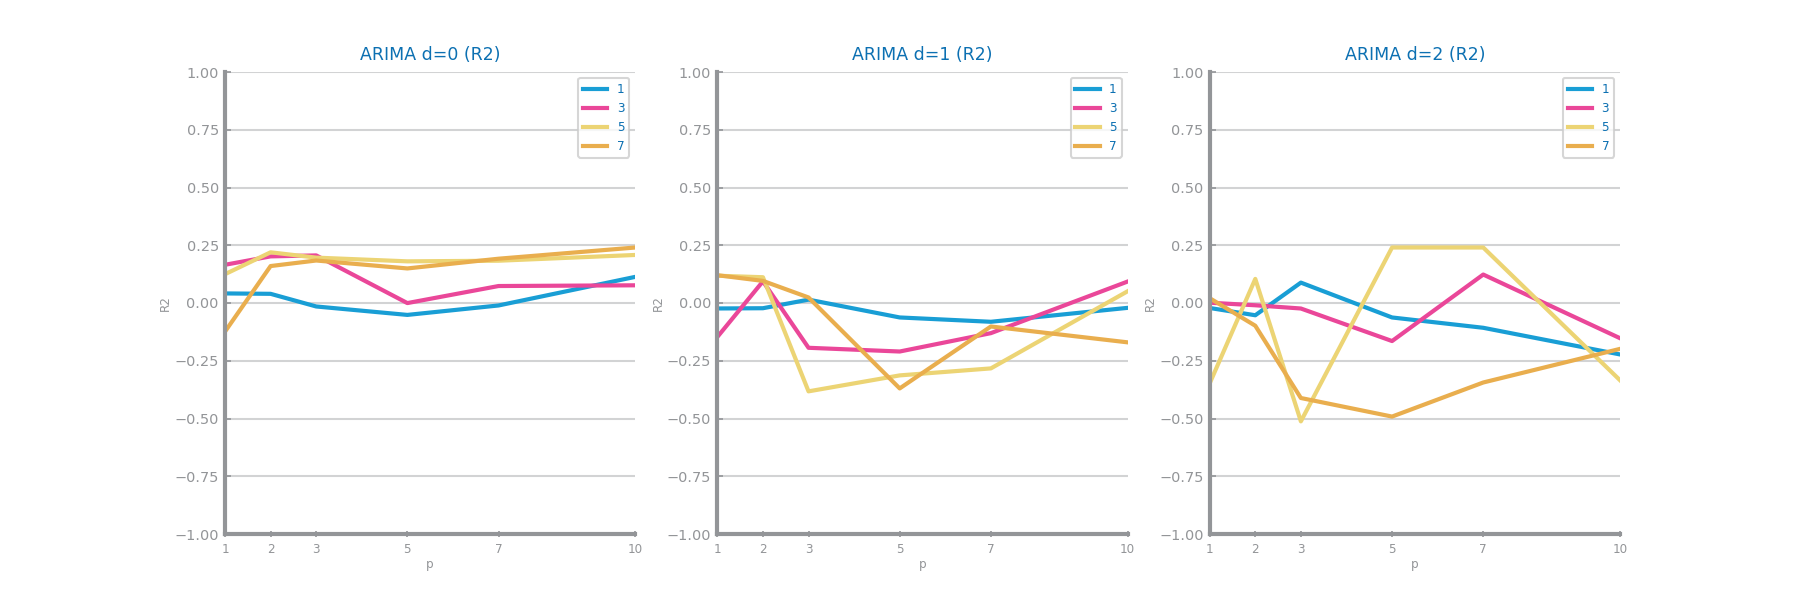
\includegraphics[width=0.9\textwidth]{economic_arima_R2_study.png}
\caption{Forecasting study over different parameterisations of the ARIMA algorithm with multiple variables over time series 2}
\end{figure}

\begin{figure}[H]
\centering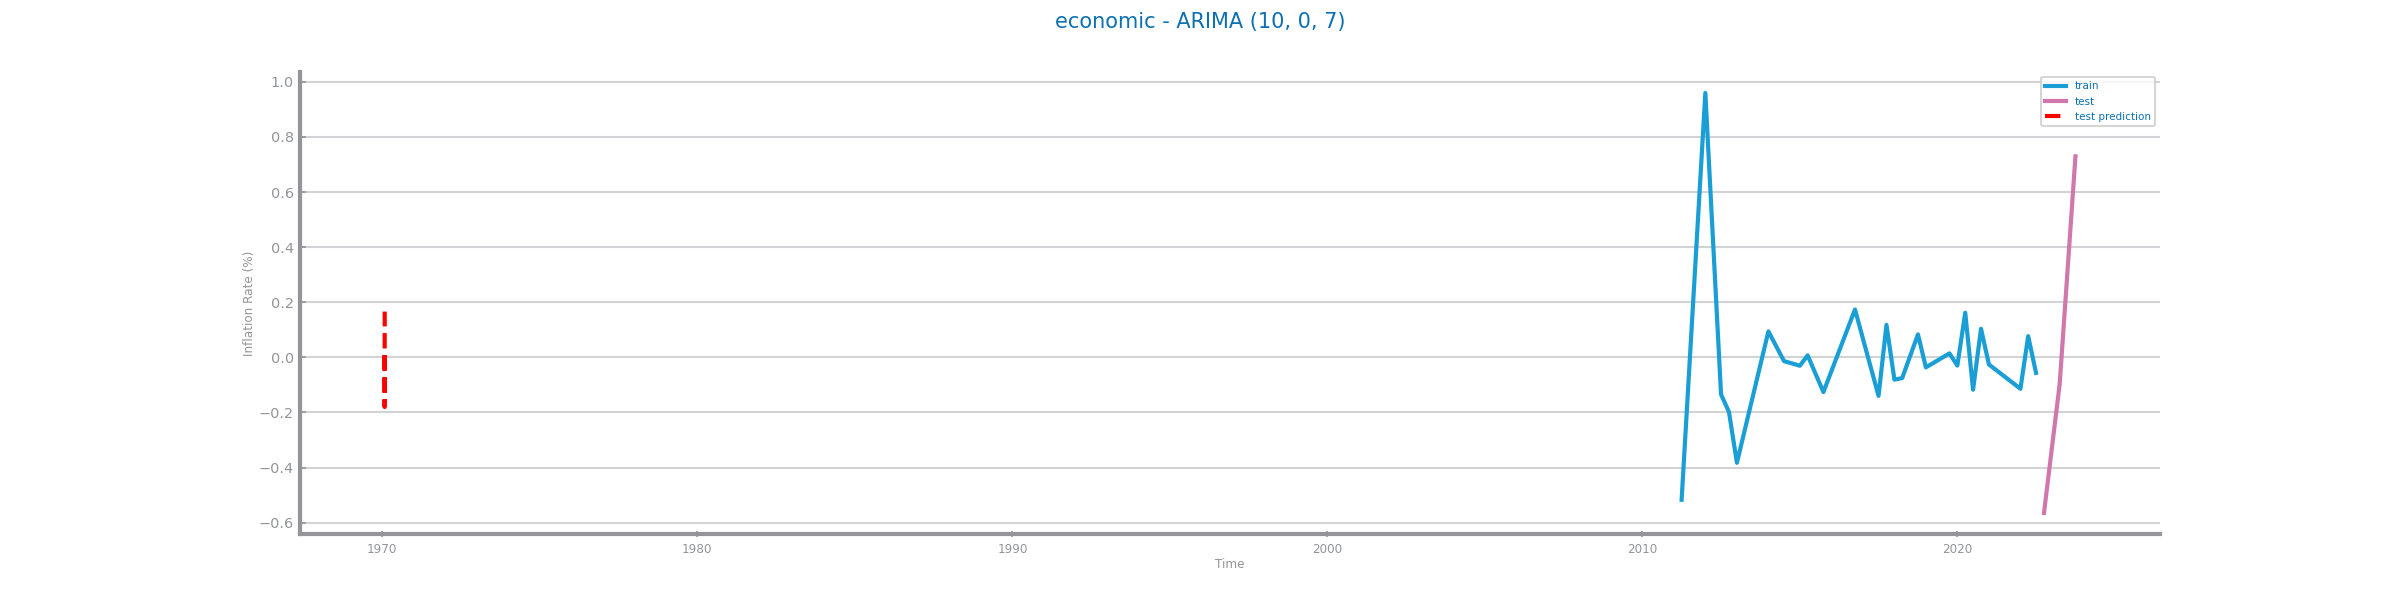
\includegraphics[width=0.9\textwidth]{economic_arima_R2_forecast.png}
\caption{Forecasting plots obtained with the best parameterisation of ARIMA algorithm with multiple variables over time series 2}
\end{figure}

\begin{figure}[H]
\centering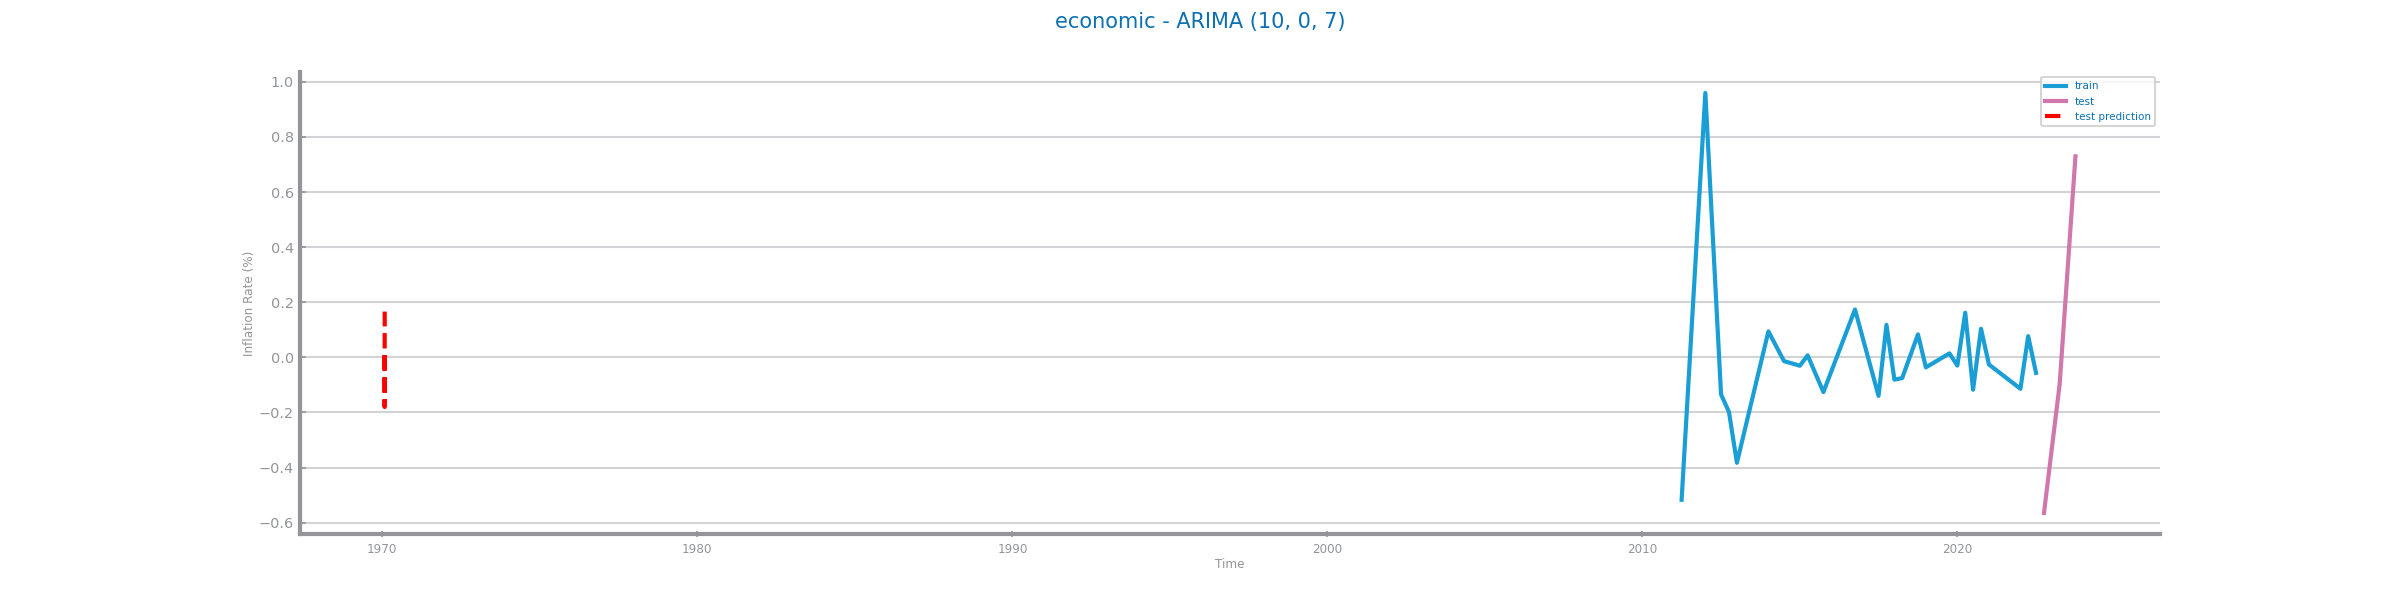
\includegraphics[width=0.9\textwidth]{economic_arima_R2_forecast.png}
\caption{Forecasting results obtained with the best parameterisation of ARIMA algorithm with multiple variables over time series 2}
\end{figure}

\subsection*{\textit{LSTMs Model}}
\ctext[RGB]{190,190,190}{Shall be used to present the results achieved through LSTMs.  \textbf{Shall not exceed 500 characters.}}

\begin{figure}[H]
\centering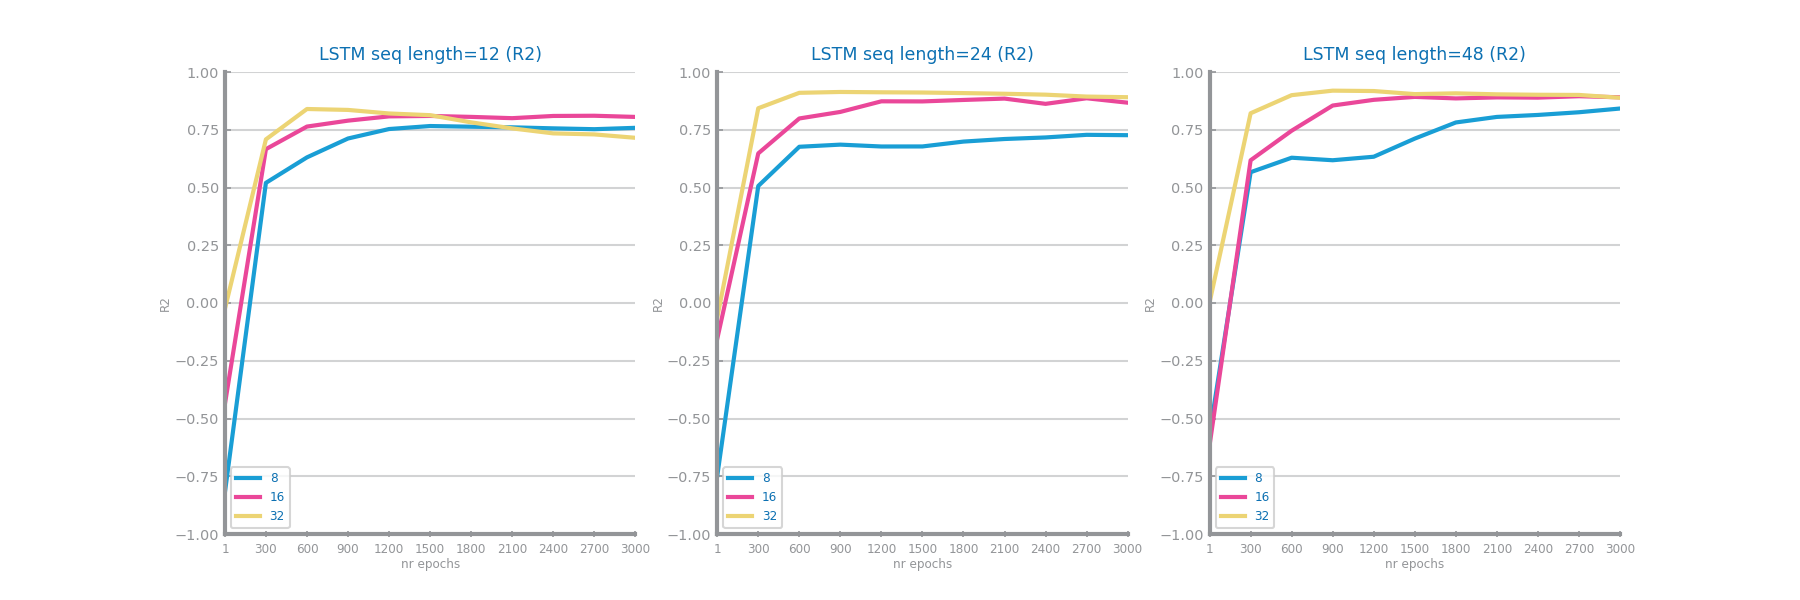
\includegraphics[width=0.9\textwidth]{TRAFFIC_lstms_R2_study.png}
\caption{Forecasting study over different parameterisations of LSTMs over time series 1, only with the target variable}
\end{figure}

\begin{figure}[H]
\centering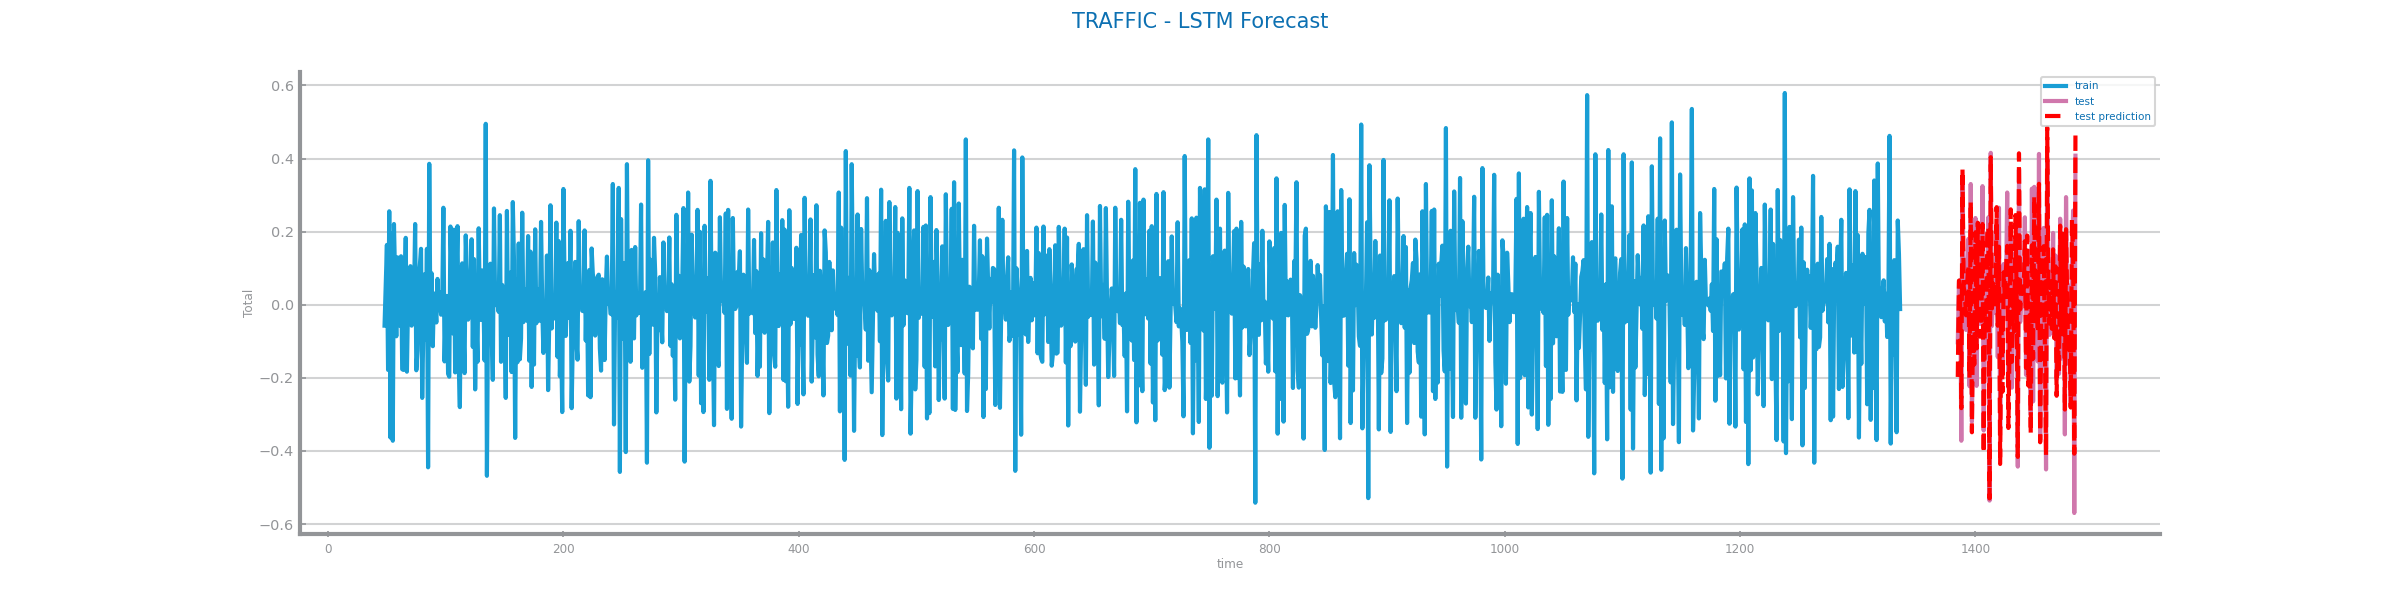
\includegraphics[width=0.9\textwidth]{TRAFFIC_lstms_R2_forecast.png}
\caption{Forecasting plots obtained with the best parameterisation of LSTMs, over time series 1, only with the target variable}
\end{figure}

\begin{figure}[H]
\centering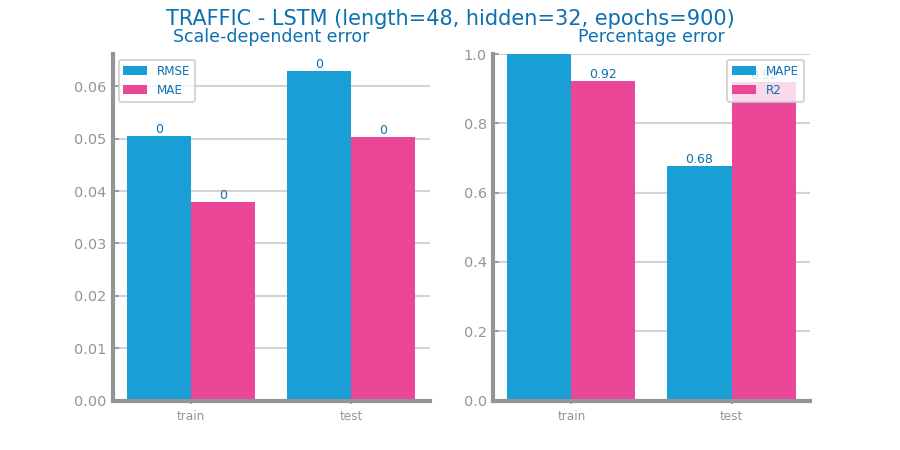
\includegraphics[width=0.9\textwidth]{TRAFFIC_lstms_R2_eval.png}
\caption{Forecasting results obtained with the best parameterisation of LSTMs, over time series 1, only with the target variable}
\end{figure}

\begin{figure}[H]
\centering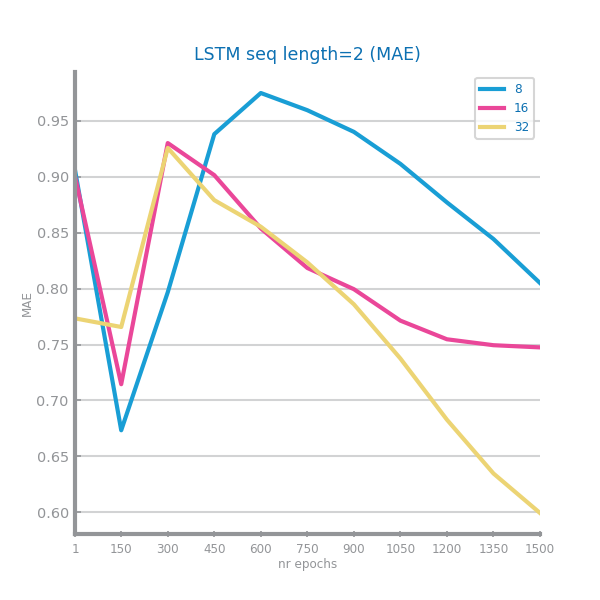
\includegraphics[width=0.9\textwidth]{ECONOMICS_lstms_MAE_study.png}
\caption{Forecasting study over different parameterisations of the LSTMs over time series 2, only with the target variable}
\end{figure}

\begin{figure}[H]
\centering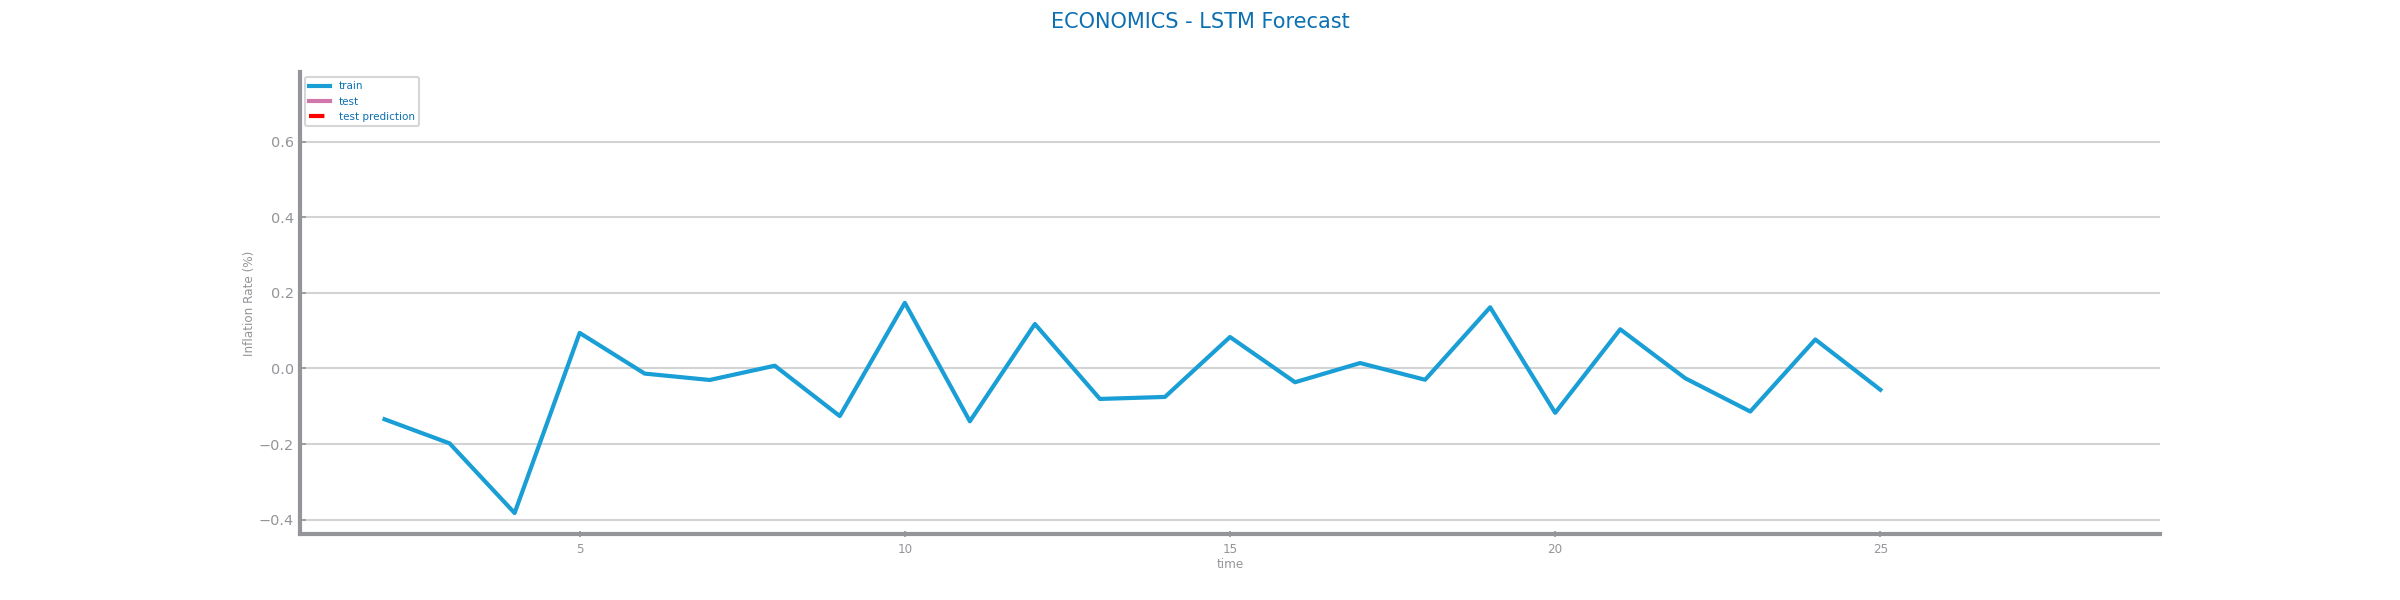
\includegraphics[width=0.9\textwidth]{ECONOMICS_lstms_MAE_forecast.png}
\caption{Forecasting plots obtained with the best parameterisation of LSTMs, over time series 2, only with the target variable}
\end{figure}

\begin{figure}[H]
\centering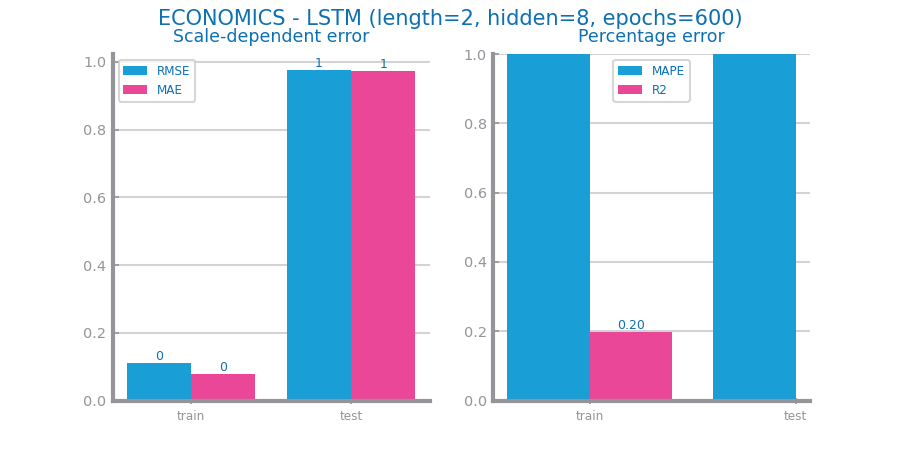
\includegraphics[width=0.9\textwidth]{ECONOMICS_lstms_MAE_eval.png}
\caption{Forecasting results obtained with the best parameterisation of LSTMs, over time series 2, only with the target variable}
\end{figure}

\begin{figure}[H]
\centering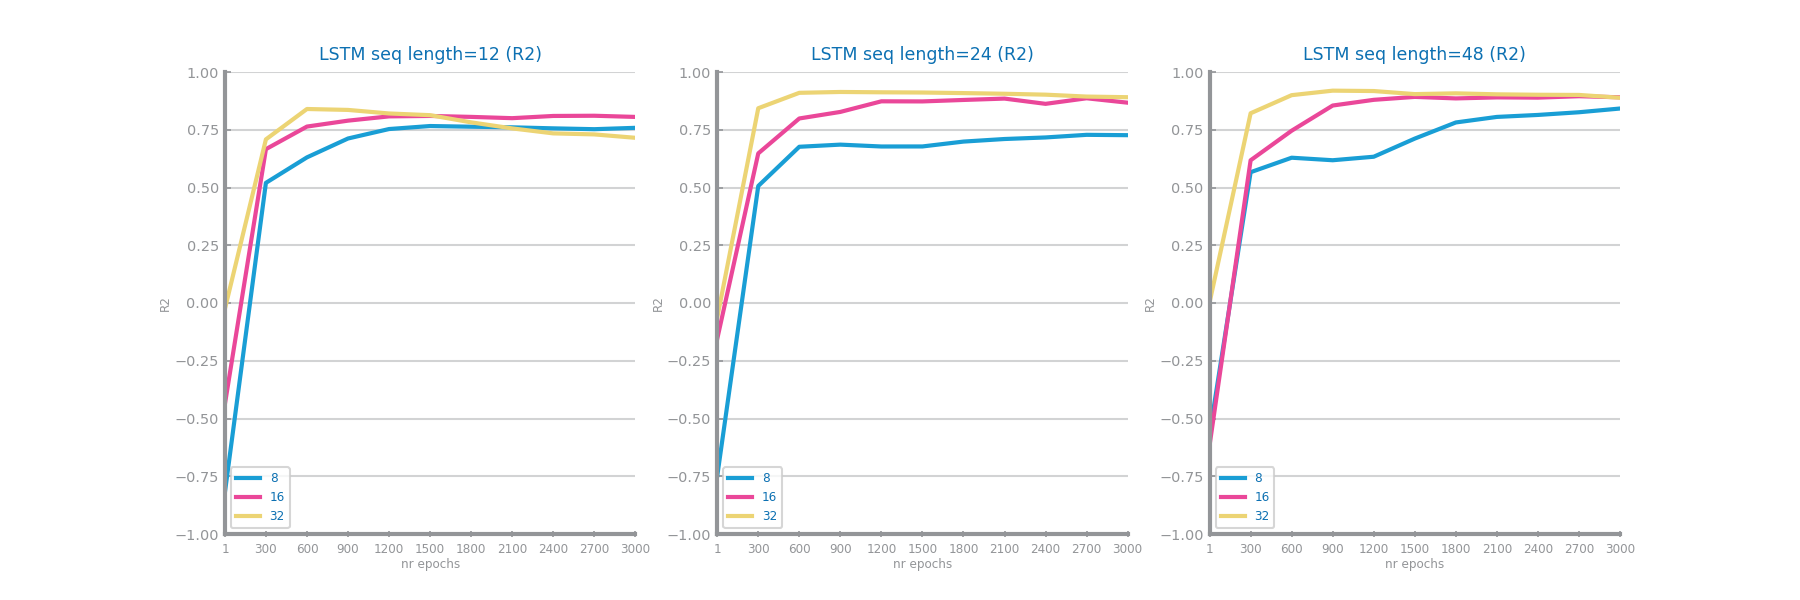
\includegraphics[width=0.9\textwidth]{TRAFFIC_lstms_R2_study.png}
\caption{Forecasting study over different parameterisations of LSTMs with multiple variables over time series 1}
\end{figure}

\begin{figure}[H]
\centering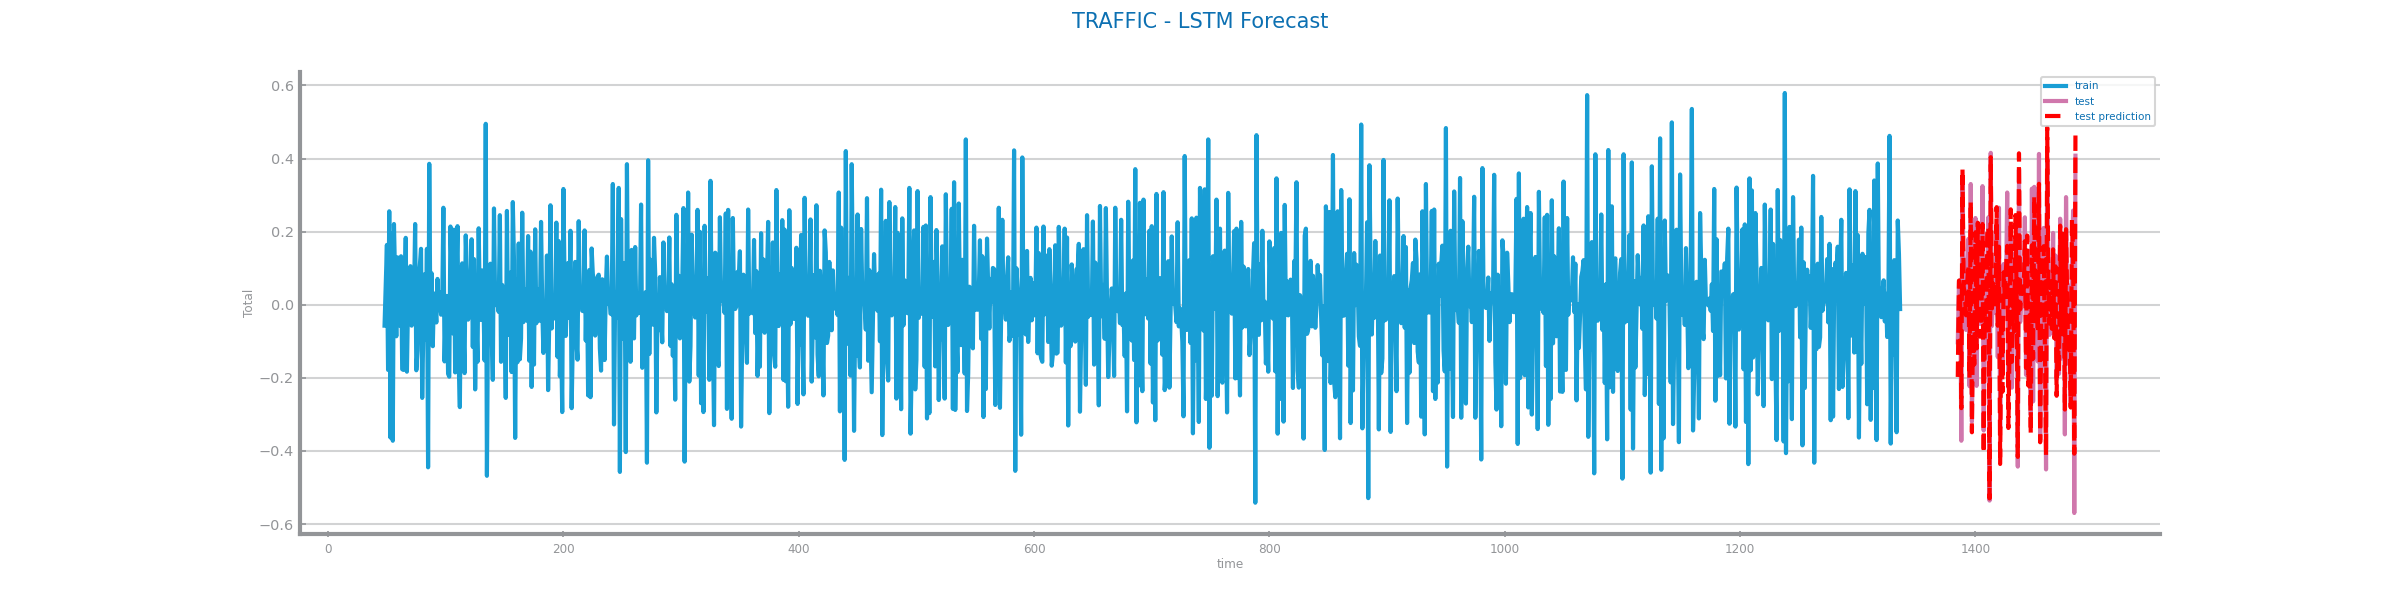
\includegraphics[width=0.9\textwidth]{TRAFFIC_lstms_R2_forecast.png}
\caption{Forecasting plots obtained with the best parameterisation of LSTMs with multiple variables over time series 1}
\end{figure}

\begin{figure}[H]
\centering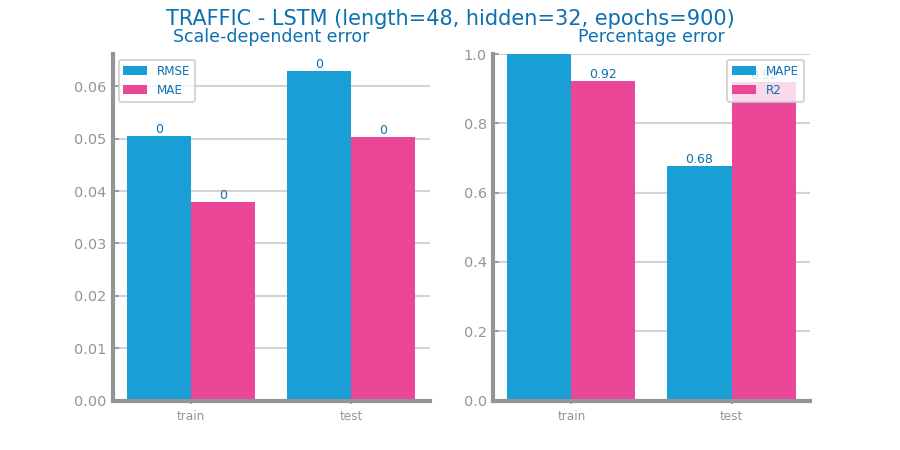
\includegraphics[width=0.9\textwidth]{TRAFFIC_lstms_R2_eval.png}
\caption{Forecasting results obtained with the best parameterisation of LSTMs with multiple variables over time series 1}
\end{figure}

\begin{figure}[H]
\centering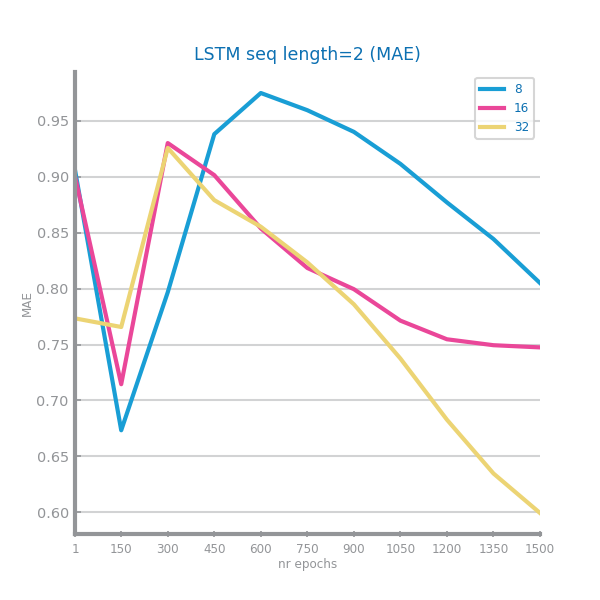
\includegraphics[width=0.9\textwidth]{ECONOMICS_lstms_MAE_study.png}
\caption{Forecasting study over different parameterisations of LSTMs with multiple variables over time series 2}
\end{figure}

\begin{figure}[H]
\centering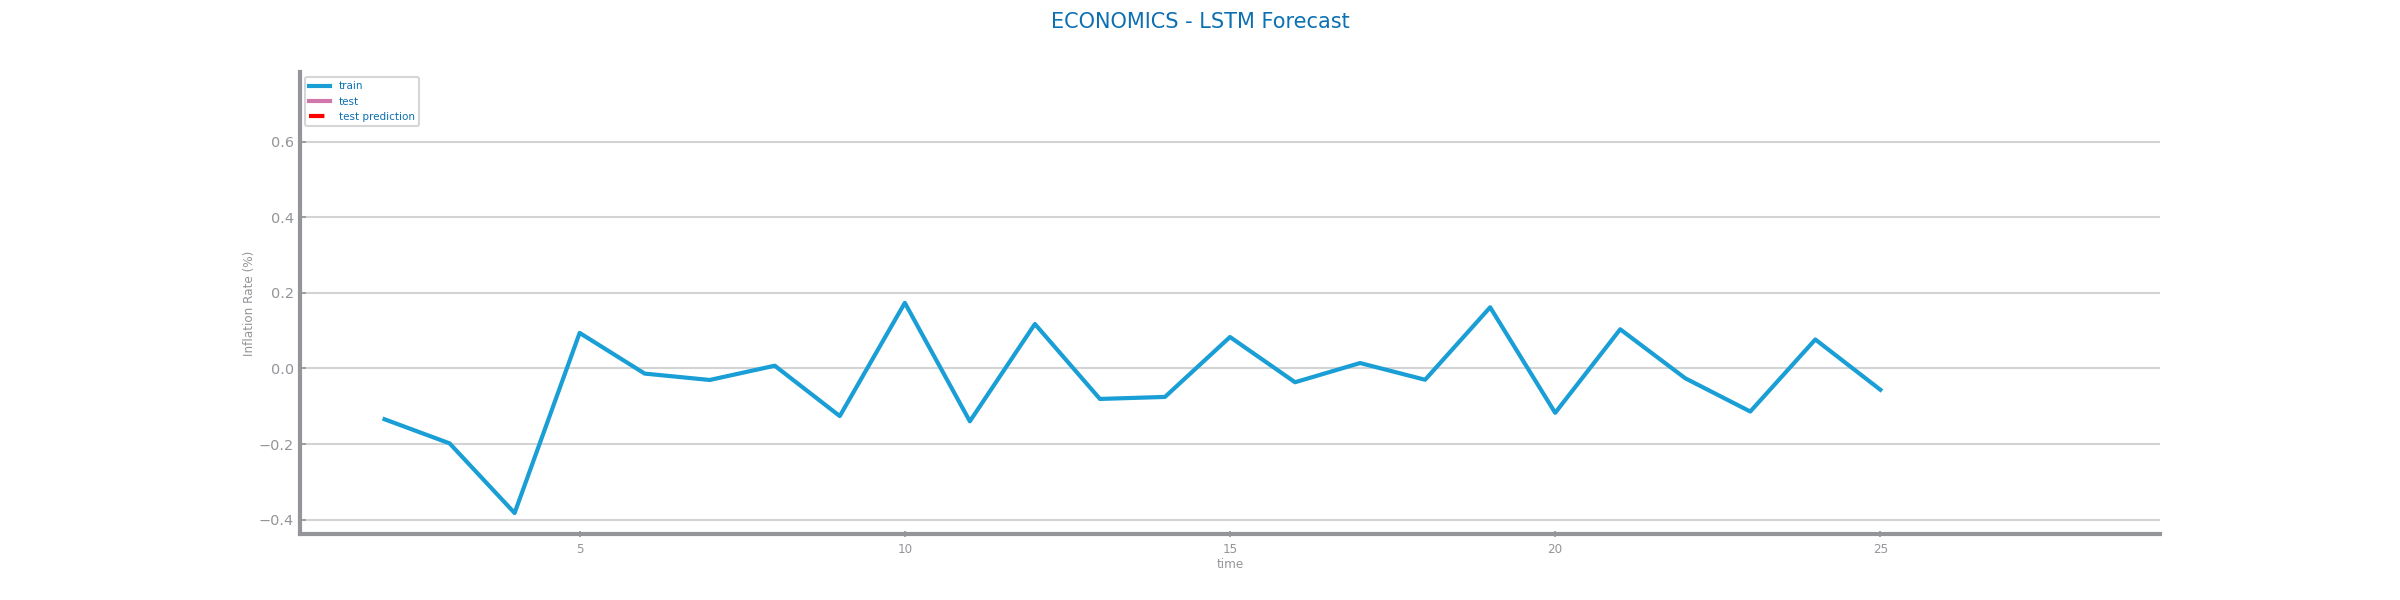
\includegraphics[width=0.9\textwidth]{ECONOMICS_lstms_MAE_forecast.png}
\caption{Forecasting plots obtained with the best parameterisation of LSTMs with multiple variables over time series 2}
\end{figure}

\begin{figure}[H]
\centering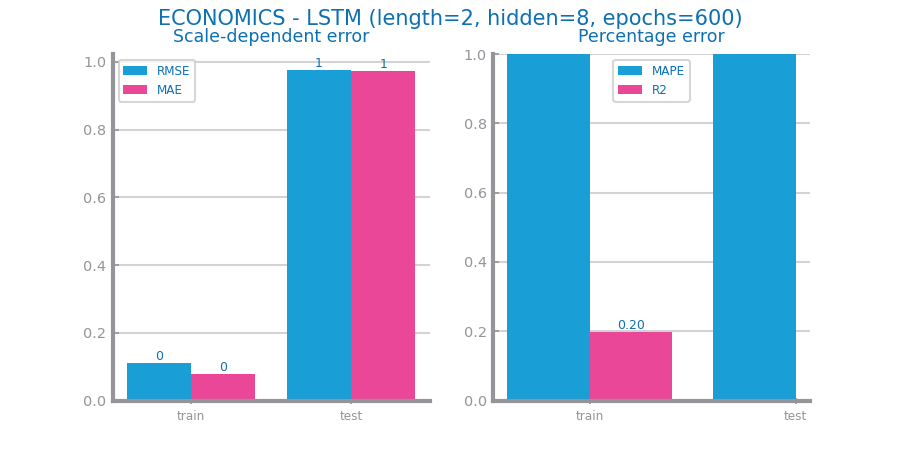
\includegraphics[width=0.9\textwidth]{ECONOMICS_lstms_MAE_eval.png}
\caption{Forecasting results obtained with the best parameterisation of LSTMs with multiple variables over time series 2}
\end{figure}

\section{CRITICAL ANALYSIS}
\ctext[RGB]{190,190,190}{Shall be used to present a summary of the results achieved with the different forecasting techniques, and the impact of the different preparation tasks on their performance. A critical assessment of the best models shall be presented, clearly stating if the models seem to be good enough for the problem at hand. Additional charts may be presented here.  \textbf{Shall not exceed 2000 characters.}}

\end{document}